% gruposlie.tex
% Fichero principal
%
% Copyright (C) 2022--2025 José A. Navarro Ramón <janr.devel@gmail.com>
% Licencia del código GPLv2
% Licencia Creative Commons Recognition Non-Commercial Share-alike.
% (CC-BY-NC-SA)

\documentclass[a4paper,oneside]{book}

% Paquetes
\usepackage{gruposlie.pkg}

% Definiciones
\usepackage{gruposlie.defs}

\begin{document}
% -----------------------------------------------------------------------------
% Portada
\thispagestyle{empty}
% portada.tex
% Portada del libro.
%
% Copyright (C) 2022 José A. Navarro Ramón <janr.devel@gmail.com>
% Licencia Creative Commons Recognition Share alike.
% (CC-BY-SA)

\titleTH


%%% Local Variables:
%%% mode: latex
%%% TeX-engine: luatex
%%% TeX-master: "../gruposlie.tex"
%%% End:

% -----------------------------------------------------------------------------
% Tabla de contenidos
\thispagestyle{empty}
% tablacontenidos.tex
% Tabla de contenidos.
%
% Copyright (C) 2022, 2023, 2024 José A. Navarro Ramón <janr.devel@gmail.com>
% Licencia Creative Commons Recognition Share alike.
% (CC-BY-SA)

\tableofcontents

%%% Local Variables:
%%% mode: latex
%%% TeX-engine: luatex
%%% TeX-master: "../gruposlie.tex"
%%% End:

% -----------------------------------------------------------------------------
\frontmatter
% prefacio.tex
%
% Copyright (C) 2022--2025 José A. Navarro Ramón <janr.devel@gmail.com>
% Licencia Creative Commons Recognition Share-alike.
% (CC-BY-SA)

\chapter{Prefacio}
Este texto consiste en unos apuntes personales tomados de unas lecciones en vídeo
publicadas en
\href{%
  https://www.youtube.com/watch?v=4NE-KNwHKSI\&list=PLAnA8FVrBl8DTFTMP8kXbDnRJHQKqfjaw
}
{Youtube}
por \href{https://www.patreon.com/JavierGarcia/}{Javier García}.

En principio he escrito el texto para que me fuera útil, aunque también lo podría ser
para otras personas.

Confecciono estos apuntes por un motivo doble: el primero es para poder repasar las
lecciones o alguna parte de ellas de forma ágil; el segundo, porque su redacción me
ayuda a asimilar mejor el contenido ---como efecto adverso , al redactarlo a mi
conveniencia se podrían generar errores e inexactitudes---.

Si alguien diera con este texto y le interesara, recomiendo que estudie primero las
lecciones en vídeo, pues tienen valor pedagógico que no se puede transcribir en unos
apuntes.

Cuando se intenta aprender esta materia de forma autodidacta, cuesta mucho avanzar y se
suele terminar perdido. El autor de las lecciones introduce los grupos de Lie partiendo
de conocimientos básicos de bachillerato o de primero de carrera y desde mi punto de
vista consigue su objetivo. En todo caso, sirven su propósito para iniciarse en los
grupos de Lie de forma efectiva, de manera que posteriormente podría ampliar estos
conocimientos.

En algunos puntos del texto he añadido algo, y en otros he eliminado alguna explicación
o desarrollo, para adaptar el texto a mi proceso de aprendizaje.

Los apuntes están confeccionados utilizando Lua\LaTeX\ y están siendo continuamente
corregidos con cada relectura del material. Por ahora no considero que estén listos para
ser publicados y los marco como un borrador.


 
%%% Local Variables:
%%% mode: latex
%%% TeX-engine: luatex
%%% TeX-master: "../gruposlie.tex"
%%% End:

% -----------------------------------------------------------------------------
% Teoría
\mainmatter
%\part{Teoría}
% grupos.tex
%
% Copyright (C) 2022--2025 José A. Navarro Ramón <janr.devel@gmail.com>
% Licencia del código GPLv2
% Licencia Creative Commons Recognition Non-Commercial Share-alike.
% (CC-BY-NC-SA)

\chapter{Grupos}

\section{Definición de grupo}
Un grupo $\{G,\cdot\,\}$ es una estructura algebraica formada por un conjunto $G$,
asociado a una operación interna '$\cdot\,$', llamada genéricamente \emph{producto}, que
asocia a cada par ordenado $(x,y)$ de elementos de $G$, un elemento $x\cdot y$ de $G$,
con las tres propiedades siguientes:
\begin{enumerate}
\item \textbf{Propiedad asociativa}. Para tres elementos cualesquiera de $G$
  \begin{equation}\label{eq:gru-asociativa}
    \forall x, y, z \in G, \quad (x \cdot y) \cdot z = x \cdot (y \cdot z)
  \end{equation}
\item \textbf{Elemento identidad}. Hay un único elemento, $e$, de $G$, llamado elemento
  identidad o neutro que, combinado con cualquier elemento del grupo, lo deja inalterado
  \begin{equation}\label{eq:gru-identidad}
    \exists !\, e \in G \ \text{tal que}\ \forall x \in G, \quad e \cdot x
    = x \cdot e = x
  \end{equation}
\item \textbf{Elemento inverso}. Todo elemento $x$ de $G$ tiene un inverso, $x^{-1}$, de
  manera que la composición de ambos produce el  elemento neutro
  \begin{equation}\label{eq:gru-inverso}
    \forall x \in G, \exists\, !\, x^{-1} \
    \text{tal que}\ x^{-1} \cdot x = x \cdot  x^{-1} = e
  \end{equation}
\end{enumerate}

Si además, la operación tuviera la propiedad conmutativa, se diría que el grupo es
\emph{conmutativo} o \emph{abeliano}:
\begin{enumerate}
\item[4.] \textbf{Propiedad conmutativa}. Para cualesquiera dos elementos $x$ e $y$ de
  $G$ se cumple que no importa el orden en el que se realice el producto
  \begin{equation}\label{eq:gru-conmutativa}
    \forall x,y \in G, \quad x \cdot y = y \cdot x
  \end{equation}
\end{enumerate}

\section{Clasificación de grupos}
Hay muchos criterios de clasificación de grupos. Por ejemplo, atendiendo a la naturaleza
de sus elementos, como grupos de simetría, etc.

Uno de estos criterios se basa en el número de elementos que lo forman: Grupos finitos,
cuando el número de elementos es finito y grupos infinitos, cuando su cardinalidad es
infinita.

\newpage
Por otro lado, atendiendo a la numerabilidad, tendremos:
\begin{itemize}
\item Grupos numerables:
  Cuando el número de elementos es finito o existe una biyección entre los elementos
  del grupo y el conjunto de enteros.
\item Grupos continuos:
  En caso contrario.
\end{itemize}

En lo que sigue nos interesarán los grupos continuos.




 
%%% Local Variables:
%%% mode: latex
%%% TeX-engine: luatex
%%% TeX-master: "../gruposlie.tex"
%%% End:

% gruposlie.tex
%
% Copyright (C) 2022--2025 José A. Navarro Ramón <janr.devel@gmail.com>
% Licencia Creative Commons Recognition Share-alike.
% (CC-BY-SA)

\chapter{Grupos de Lie}
A bocajarro, definimos brevemente un grupo de Lie como un grupo que es una variedad
diferenciable, donde las operaciones del grupo son suaves o analíticas. Su estructura
es continua y \emph{suavemente deformable}. Más adelante se definirá de forma más
precisa.

Los grupos de Lie tienen mucha importancia en matemáticas y en física.
Aquí estamos interesados, principalmente, en su aplicación a la mecánica cuántica; en
particular, para comprender el concepto de spin en física de partículas, que en algunos
textos elementales se identifica incorrectamente con el giro de las partículas alrededor
de su eje.

\section{Rotaciones en el plano}
Para asimilar mejor el concepto de \emph{grupo de Lie}, empezamos analizando las rotaciones en $\symbb{R}^2$, olvidándonos por un momento de los grupos.
Las caracterizaremos de dos formas diferentes:
\begin{enumerate}
\item Mediante consideraciones trigonométricas.
\item Mediante una transformación que mantiene invariante la longitud.
\end{enumerate}

\subsection{Caracterización trigonométrica}
En la figura~\ref{fig:gli-x_axes} se representa un sistema de coordenadas cartesianas
rectangulares\footnotemark{} y un punto P cualquiera del espacio, con coordenadas
$(x_1,x_2)$, donde $\vvv{r}$ es el vector que indica su posición con respecto al origen.
\footnotetext{Denotamos los ejes de $\symbb{R}^2$ mediante $x_1$ y $x_2$,   igual que
  las coordenadas del punto. El lector no debería confundirlos, su interpretación se
  desprende del contexto.}
Las coordenadas de P con respecto a este sistema son
\begin{subequations}
  \begin{align}\label{eq:gli-coordxuno}
    x_1 &= r \cos(\alpha+\beta)\\
    \label{eq:gli-coordxdos}
    x_2 &= r \sin(\alpha+\beta)
  \end{align}
\end{subequations}
\begin{figure}[ht]
  \centering
  \begin{minipage}{0.40\linewidth}
    % Escala
    \def\scl{1}
    % Eje x
    \pgfmathsetmacro{\XMLONG}{0}
    \pgfmathsetmacro{\XPLONG}{3}
    % Eje y
    \pgfmathsetmacro{\YMLONG}{0}
    \pgfmathsetmacro{\YPLONG}{3}
    % Vector P
    \pgfmathsetmacro{\PMOD}{2.5}
    \pgfmathsetmacro{\PANG}{50}
    % Fondo
    \pgfmathsetmacro{\HORZ}{0.40}
    \pgfmathsetmacro{\VERT}{0.24}
    \pgfmathsetmacro{\MOD}{sqrt(\HORZ^2 + \VERT^2)}
    \pgfmathsetmacro{\ANGSD}{atan(\VERT / \HORZ)}
    \pgfmathsetmacro{\ANGII}{\ANGSD + 180.0}
    %
    \centering
    \begin{tikzpicture}[%
      scale=\scl,
      baseline,
      every node/.style={black,font=\small},
      eje/.style={->},
      vector/.style={-{Latex}, shorten >=1.2pt, line width=.8pt},
      dimmed/.style={lightgray, line width=.8pt, dotted},
      background/.style={
        line width=\bgborderwidth,
        draw=\bgbordercolor,
        fill=\bgcolor,
      },
      ]
      % Coordenadas
      \coordinate (O) at (0,0);
      \coordinate (xini) at (-\XMLONG cm,0);
      \coordinate (xfin) at (\XPLONG cm,0);
      \coordinate (yini) at (0,-\YMLONG cm);
      \coordinate (yfin) at (0,\YPLONG cm);
      \coordinate (P) at (\PANG:\PMOD cm);
      \path (O) -- coordinate (OPmidway) (P);
      % Ángulo alfa + beta
      \path (xfin) -- (O) -- (P)
%      pic [draw=black,fill=black!20,"\footnotesize $\alpha + \beta$",angle radius=6.3mm,
%      angle eccentricity=1.6,-{Latex[length=1.4mm,scale=.9,bend]}]
%      {angle = xfin--O--P};
      pic [draw=black,fill=black!20,"\footnotesize $\alpha + \beta$",angle radius=6.3mm,
      angle eccentricity=1.6]
      {angle = xfin--O--P};
      % Ejes
      \draw[eje] (xini) -- (xfin);
      \node[right, name=letraejex] at (xfin) {$x_1$};
      \coordinate (below) at ($(letraejex) - (0,1.0em)$);
      \draw[eje] (yini) -- (yfin);
      \node[above, name=letraejey] at (yfin) {$x_2$};
      \coordinate (left) at ($(letraejey) - (1.3em,0)$);
      % Vector de posición del punto P
      % \draw[black!70,-{Latex},shorten >=1.2pt] (O) -- (P);
      \draw[vector] (O) -- (P);
      \path (P |- xfin) coordinate (xm);
      \path (P -| yfin) coordinate (ym);
      \draw[dimmed] (P) -- (xm);
      \draw[dimmed] (P) -- (ym);
      \node[below] at (xm) {$x_1$};
      \node[left] at (ym) {$x_2$};
      \node[above=5pt] at (OPmidway) {$\vvv{r}$};
      % Punto
      \fill[fill=red,draw=black] (P) circle [radius=1.4pt];
      \node[above right] at (P) {$P$};
      % Origen
      \filldraw (O) circle [radius=.2pt];
      % Fondo amarillo
      \path (current bounding box.south west) ++(\ANGII:\MOD) coordinate (SW);
      \path (current bounding box.north east) ++(\ANGSD:\MOD) coordinate (NE);
      % \filldraw[draw=black, fill=red] (NE) circle[radius=1pt];
      \begin{scope}[on background layer]
        \draw[background] (SW) rectangle (NE);
      \end{scope}
    \end{tikzpicture}
    \caption{Ejes originales sin girar y punto P del plano, de coordenadas $(x_1,x_2)$.}
    \label{fig:gli-x_axes}
  \end{minipage}
  \hspace{1em}
  \begin{minipage}{0.45\linewidth}
    % Escala
    \def\scl{1}
    % Eje x
    \pgfmathsetmacro{\XMLONG}{0}
    \pgfmathsetmacro{\XPLONG}{3}
    % Eje y
    \pgfmathsetmacro{\YMLONG}{0}
    \pgfmathsetmacro{\YPLONG}{3}
    % Vector P
    \pgfmathsetmacro{\PMOD}{2.5}
    \pgfmathsetmacro{\PANG}{55}
    % Ángulo rotado
    \pgfmathsetmacro{\ANGROT}{20}
    \pgfmathsetmacro{\ANGROTPLUSNINETY}{\ANGROT + 90}
     % Fondo
    \pgfmathsetmacro{\HORZ}{0.25}
    \pgfmathsetmacro{\VERT}{0.35}
    \pgfmathsetmacro{\MOD}{sqrt(\HORZ^2 + \VERT^2)}
    \pgfmathsetmacro{\ANGSD}{atan(\VERT / \HORZ)}
    \pgfmathsetmacro{\ANGII}{\ANGSD + 180.0}
    % 
    \centering
    \begin{tikzpicture}[%
      scale=\scl,
      every node/.style={black,font=\small},
      ejerotado/.style={->},
      eje/.style={->, black!35},
      vector/.style={-{Latex}, shorten >=1.2pt, line width=.8pt},
      dimmed/.style={lightgray, line width=.8pt, dotted},
      background/.style={
        line width=\bgborderwidth,
        draw=\bgbordercolor,
        fill=\bgcolor,
      },      
      ]
      % Coordenadas
      \coordinate (O) at (0,0);
      \coordinate (xini) at (-\XMLONG cm,0);
      \coordinate (xfin) at (\XPLONG cm,0);
      \coordinate (yini) at (0,-\YMLONG cm);
      \coordinate (yfin) at (0,\YPLONG cm);
      \coordinate (x'ini) at (-\ANGROT:\XMLONG);
      \coordinate (x'fin) at (\ANGROT:\XPLONG);
      \coordinate (y'ini) at (-\ANGROTPLUSNINETY:\YMLONG);
      \coordinate (y'fin) at (\ANGROTPLUSNINETY:\YPLONG);
      \coordinate (P) at (\PANG:\PMOD cm);
      \path (O) -- coordinate (OPmidway) (P);
      % Ángulo alfa
      \path (xfin) -- (O) -- (x'fin) pic
      [draw=black,fill=green!30,"$\alpha$",angle radius=7mm,
      angle eccentricity=1.3,-{Latex[length=1.4mm,scale=.9,bend]}]
      {angle = xfin--O--x'fin};
      % Ángulo beta
      \path (x'fin) -- (O) -- (P) pic
      [draw=black!50!,fill=black!20,"$\beta$",angle radius=7mm, angle
      eccentricity=1.3] {angle = x'fin--O--P};
      % Ejes originales
      \draw[eje] (xini) -- (xfin);
      \node[right, name=letraejex, black!35] at (xfin) {$x_1$};
      \coordinate (below) at ($(letraejex) - (0,1.0em)$);
      \draw[eje] (yini) -- (yfin);
      \node[above, name=letraejey, black!35] at (yfin) {$x_2$};
      % Ejes rotados
      \draw[ejerotado] (O) -- (x'fin);
      % \path (O) -- node[pos=1.08,name=letraejexprima] {$x_1'$} (x'fin);
      \path (O) -- node[pos=1.08] {$x_1'$} (x'fin);
      \draw[ejerotado] (O) -- (y'fin);
      \path (O) -- node[pos=1.08] {$x_2'$} (y'fin);
      \path ($(O)!(P)!(x'fin)$) coordinate (x'm);
      \path ($(O)!(P)!(y'fin)$) coordinate (y'm);

      \draw[dimmed] (x'm) -- (P);
      \node[below, rotate=\ANGROT] at (x'm) {$x'_1$};
      \draw[dimmed] (y'm) -- (P);
      \node[left, rotate=\ANGROT] at (y'm) {$x'_2$};
      % Punto
      \draw[vector] (O) -- (P);
      \node[above=5pt] at (OPmidway) {$\vvv{r'}$};
      \fill[fill=red,draw=black] (P) circle [radius=1.4pt];
      \node[above right] at (P) {$P$};
      % Origen
      \filldraw (O) circle [radius=.2pt];
      % Fondo amarillo
      \path (current bounding box.south west) ++(\ANGII:\MOD) coordinate (SW);
      \path (current bounding box.north east) ++(\ANGSD:\MOD) coordinate (NE);
      % \filldraw[draw=black, fill=red] (NE) circle[radius=1pt];
      \begin{scope}[on background layer]
        \draw[background] (SW) rectangle (NE);
      \end{scope}      
    \end{tikzpicture}
    \caption{Ejes rotados un ángulo $\alpha$.
      Las coordenadas de P con respecto a estos nuevos ejes son $(x'_1,x'_2)$.}
    \label{fig:gli-rotated_axes}
  \end{minipage}
\end{figure}

En la figura~\ref{fig:gli-rotated_axes} llevamos a cabo una
\emph{rotación pasiva}\footnotemark{}, girando los ejes un ángulo $\alpha$ en sentido
positivo (antihorario).
Observe que no cambia la distancia, $r$, entre el punto y el origen, esto es, r'=r.
\footnotetext{En una rotación pasiva se gira el punto de vista (el sistema de
  referencia) y no el punto.}
Las coordenadas del punto P con respecto del sistema girado son
\begin{subequations}
  \begin{align}\label{eq:gli-coordxprimauno}
    x_1' &= r \cos\beta\\
    \label{eq:gli-coordxprimados}
    x_2' &= r \sin\beta
  \end{align}
\end{subequations}

Desarrollamos~\eqref{eq:gli-coordxuno} y~\eqref{eq:gli-coordxdos} y
utilizamos~\eqref{eq:gli-coordxprimauno} y~\eqref{eq:gli-coordxprimados}
\begin{align*}
  x_1 &= r \cos\alpha \cos\beta - r \sin\alpha \sin\beta
        = \cos\alpha\,(r\cos\beta) - \sin\alpha\,(r\sin\beta)\\
        &= \cos\alpha\cdot x_1' - \sin\alpha \cdot x_2'\\
  x_2 &= r \sin\alpha \cos\beta + r \cos\alpha \sin\beta
        = \sin\alpha\,(r \cos\beta) + \cos\alpha\,(r \sin\beta)\\
        &= \sin\alpha \cdot x_1' + \cos\alpha \cdot x_2'
\end{align*}

Estas dos últimas expresiones se pueden representar en forma matricial
\[
  \begin{pmatrix}
    x_1 \\[0.4ex] x_2
  \end{pmatrix}
  =
  \begin{pmatrix}
    \cos\alpha & -\sin\alpha\\[0.3ex] \sin\alpha & \cos\alpha
  \end{pmatrix}
  \begin{pmatrix}
    x_1' \\[0.3ex] x_2'
  \end{pmatrix}
\]

Llamando $\mmm{M}$ a la matriz de la transformación, $\vvv{x}$ y $\vvv{x'}$
a los vectores que representan las coordenadas del punto sin rotar y rotado,
respectivamente, la ecuación anterior queda
\begin{equation}\label{eq:gli-rotpasiva_inversa_vectores}
  \vvv{x} = \mmm{M} \vvv{x'}
\end{equation}

Estamos interesados en la transformación inversa, esto es,
queremos hallar las nuevas coordenadas de P respecto al sistema
girado si conocemos las que tiene el punto en el sistema original,
$\vvv{x'} = \mmm{R} \vvv{x}$, donde $\mmm{R}$ será la matriz de rotación
pasiva.
Para resolver la ecuación anterior, hay que multiplicar por la
izquierda\footnotemark{} la inversa de la matriz $\mmm{M}$ en la
ecuación~\eqref{eq:gli-rotpasiva_inversa_vectores}
\footnotetext{Se multiplica por la izquierda porque las matrices cuadradas
  junto con el producto de matrices, forman un grupo no conmutativo.}
\[
  \mmm{M}^{-1}\vvv{x} = \mmm{M}^{-1}\mmm{M}\vvv{x'}
\]
\[
  \mmm{M}^{-1}\vvv{x} = \mmm{I}\vvv{x'}
\]
\[
  \vvv{x'} = \mmm{M}^{-1}\vvv{x}
\]
Y como
\[
  \vvv{x'} = \mmm{R}\vvv{x}
\]
Se deduce que la matriz de rotación pasiva es la inversa de $\mmm{M}$
\[
  \mmm{R} = \mmm{M}^{-1}
\]

Antes de nada, debemos comprobar que la matriz $\mmm{M}$ tiene inversa; para ello su
determinante no puede ser nulo\footnotemark{}.
\footnotetext{Una matriz con determinante cero se llama \emph{matriz singular}
  y no tiene inversa.}

Calculamos el determinante y comprobamos que no es nulo, por lo que tiene inversa
\begin{equation}\label{eq:gli-determinante_M}
  \det \mmm{M}
  =
  \begin{vmatrix}
    \cos\alpha & -\sin\alpha \\ \sin\alpha & \cos\alpha
  \end{vmatrix}
  = \cos^2\alpha + \sin^2\alpha = 1
\end{equation}

La inversa de una matriz es igual a la adjunta de la traspuesta dividida entre su
determinante
\[
  \mmm{M}^{-1} = \dfrac{1}{\det(\mmm{M})}\,\text{adj} \left(\mmm{M}^\trasp\right)
\]

 Nuestra matriz $\mmm{M}$ es
\[
  \mmm{M}
  =
  \begin{pmatrix}
    \cos\alpha & -\sin\alpha\\ \sin\alpha & \cos\alpha
  \end{pmatrix}
\]

Primero hallamos la traspuesta, que se obtiene al intercambiar filas por columnas
\[
  \mmm{M}^\trasp
  =
  \begin{pmatrix}
    B_{11} & B_{12}\\ B_{21} & B_{22}
  \end{pmatrix}
  =
  \begin{pmatrix}
    \cos\alpha & \sin\alpha\\ -\sin\alpha & \cos\alpha
  \end{pmatrix}
\]

Vamos a obtener la adjunta (o de los cofactores) de la traspuesta, razonando elemento
por elemento --ya que no se hace muy pesado, por tener solo cuatro elementos--
\[
  \text{adj}\left(\mmm{M^\trasp}\right)
    = \begin{pmatrix}
        A_{11} & A_{12} \\ A_{21} & A_{22}
      \end{pmatrix}
\]

El cofactor, $A_{ij}$, de cada elemento $B_{ij}$ se obtiene multiplicando $(-1)^{\,i+j}$
por el menor complementario de $B_{ij}$.
El menor complementario es el determinante que queda al eliminar la fila $i$ y la $j$ de
la matriz.

Calculamos el cofactor de cada uno de los elementos de la matriz traspuesta. El elemento
lo indicamos con letras en rojo. En este caso, debido a que la matriz es $2\times 2$, el
menor complementario es un determinante formado por un único elemento, que no se marca
con fondo rojo
\begin{align*}
  A_{11}
  &= \text{cof}\,(B_{11})
    = (-1)^{1+1}\,\text{det}
    \begin{pNiceArray}{rr}
      \textcolor{red!80!black}{\cos\alpha} & \textcolor{black!70}{\sin\alpha}\\
      \textcolor{black!70}{-\sin\alpha} & \cos\,\alpha
      \CodeAfter
      \tikz \draw[red,line width=10pt,opacity=0.15] (1.5-|1) -- (1.5-|last);
      \tikz \draw[red,line width=30pt,opacity=0.15] (1.5|-1) -- (1.5|-last);
    \end{pNiceArray}
    = \text{det}\,(\cos\alpha)
    = \cos\alpha\\
  A_{12}
  &= \text{cof}\,(B_{12})
    = (-1)^{1+2}\,\text{det}
    \begin{pNiceArray}{rr}
      \textcolor{black!70}{\cos\alpha} & \textcolor{red!80!black}{\sin\alpha}\\
      \textcolor{black}{-\sin\alpha} & \textcolor{black!70}{\cos\alpha}
      \CodeAfter
      \tikz \draw[red,line width=10pt,opacity=0.15] (1.5-|1) -- (1.5-|last);
      \tikz \draw[red,line width=30pt,opacity=0.15] (2.5|-1) -- (2.5|-last);
    \end{pNiceArray}
    = - \text{det}\,(-\sin\alpha)
    = \sin\alpha\\
  A_{21}
  &= \text{cof}\,(B_{21})
    = (-1)^{2+1}\,\text{det}
    \begin{pNiceMatrix}
      \textcolor{black!70}{\cos\alpha} & \textcolor{black}{\sin\alpha}\\
      \textcolor{red!80!black}{-\sin\alpha} & \textcolor{black!70}{\cos\alpha}
      \CodeAfter
      \tikz \draw[red,line width=10pt,opacity=0.15] (2.5-|1) -- (2.5-|last);
      \tikz \draw[red,line width=30pt,opacity=0.15] (1.5|-1) -- (1.5|-last);
    \end{pNiceMatrix}
    = -\text{det}\,(\sin\alpha)
    = -\sin\alpha\\
  A_{22}
  &= \text{cof}\,(B_{22})
    = (-1)^{2+2}\,\text{det}
    \begin{pNiceMatrix}
      \textcolor{black}{\cos\alpha} & \textcolor{black!70}{\sin\alpha}\\
      \textcolor{black!70}{-\sin\alpha} & \textcolor{red!80!black}{\cos\alpha}
      \CodeAfter
      \tikz \draw[red,line width=10pt,opacity=0.15] (2.5-|1) -- (2.5-|last);
      \tikz \draw[red,line width=30pt,opacity=0.15] (2.5|-1) -- (2.5|-last);
    \end{pNiceMatrix}
    = \det\,(\cos\alpha)
    = \cos\alpha
\end{align*}

La matriz de cofactores de la traspuesta resulta
\[
  \text{adj} (\mmm{M}^\trasp)
  =
  \begin{pmatrix}
    A_{11} & A_{12}\\ A_{21} & A_{22}
  \end{pmatrix}
  =
  \begin{pmatrix}
    \cos\alpha & \sin\alpha\\
    -\sin\alpha & \cos\alpha
  \end{pmatrix}
\]
Teniendo en cuenta que el determinante de la matriz valía la unidad, ver
\eqref{eq:gli-determinante_M}, la matriz inversa es
\[
  \mmm{M}^{-1}
  =
  \dfrac{1}{\det(\mmm{M})}\,
  \begin{pmatrix}
    \cos\alpha & \sin\alpha\\
    -\sin\alpha & \cos\alpha
  \end{pmatrix}
  =
  \dfrac{1}{1}\,
  \begin{pmatrix}
    \cos\alpha & \sin\alpha\\
    -\sin\alpha & \cos\alpha
  \end{pmatrix}
  =
  \begin{pmatrix}
    \cos\alpha & \sin\alpha\\
    -\sin\alpha & \cos\alpha
  \end{pmatrix}
\]

Es instructivo señalar que, en este caso, la inversa es igual a la traspuesta y resulta
ser la matriz de rotación pasiva $\mmm{R}$ que buscamos
\begin{equation}
  \label{eq:gli-matriz_rotacion_2x2}
  \mmm{R}
  =
  \mmm{M}^{-1}
  =
  \mmm{M}^\trasp
  =
  \begin{pmatrix}
    \cos\alpha & \sin\alpha\\
    -\sin\alpha & \cos\alpha
  \end{pmatrix}
\end{equation}

Las nuevas coordenadas, $\vvv{x'}$, se obtienen aplicando la matriz de rotación a las
del sistema sin girar, $\vvv{x}$
\[
  \vvv{x'} = \mmm{R} \vvv{x}
\]

\[
  \begin{pmatrix}
    x'_1\\[0.4ex]x'_2
  \end{pmatrix}
  =
  \begin{pmatrix}
    \cos\alpha & \sin\alpha\\
    -\sin\alpha & \cos\alpha
  \end{pmatrix}
  \,
  \begin{pmatrix}
    x_1 \\ x_2
  \end{pmatrix}
\]

\subsubsection{Criterio de la suma de Einstein}
Abandonamos por un instante nuestro guión para explicar la notación de Einstein.
Supongamos que queremos calcular las coordenadas $\vvv{x'}$ mediante el producto
matricial
\[
  \begin{pmatrix}
    x'_1\\[0.4ex] x'_2
  \end{pmatrix}
  =
  \begin{pmatrix}
    R_{11} & R_{12}\\
    R_{21} & R_{22}
  \end{pmatrix}
  \,
  \begin{pmatrix}
    x_1 \\ x_2
  \end{pmatrix}  
\]
\begin{align*}
  x'_1 &= R_{11} x_1 + R_{12} x_2\\
  x'_2 &= R_{21} x_1 + R_{22} x_2
\end{align*}

Obtenemos que el elemento $x'_i$ de $\vvv{x'}$ se calcula mediante un sumatorio
\begin{equation}\label{eq:gli-sumatorio}
  x'_i = \sum_{j=1}^2 R_{ij} x_j
  \hspace*{3em}
  (i = 1,2)
\end{equation}

Observamos que el índice de la suma es el que se repite (el $j$ en este caso),
por lo que podemos eliminar el símbolo del sumatorio siempre que
consideremos que hay que aplicarlo cuando aparezcan índices repetidos
\begin{equation}\label{eq:gli-criteriosumaeinstein}
  x'_i = R_{ij} x_j
  \hspace*{3em}
  (i = 1,2)
\end{equation}

Cuando se utiliza el criterio de la suma de Einstein, las expresiones son más
fáciles de escribir; en nuestro caso, las~\eqref{eq:gli-criteriosumaeinstein}
son totalmente equivalentes a las~\eqref{eq:gli-sumatorio}.

\subsection[Mediante transformación que deja invariante la longitud]
{Caracterización por medio de una transformación que deja invariante la
  longitud}\label{invariante_longitud}
Ahora nos olvidaremos de la trigonometría y deduciremos las características de la matriz
de rotación $\mmm{R}$ de una manera más sofisticada.

Cuando se realiza una rotación, las distancias se deben conservar.
En nuestro ejemplo de la figura~\ref{fig:gli-rotated_axes}, la distancia $r = |\vvv{r}|$
del origen al punto es la misma en cualquiera de los sistemas de coordenadas, el
original y el girado.

Abordaremos este apartado de dos formas; en la primera, desarrollaremos los cálculos con
todo detalle y, en la segunda, seguiremos un razonamiento aún más sofisticado y potente.

\subsubsection{Desarrollo con gran detalle}
Llamemos $s$ a la distancia que se conserva, por ejemplo la distancia entre el punto P y
el origen en la figura~\eqref{fig:gli-rotated_axes}
\[
  s = \sqrt{x'^2_1 + x'^2_2}
  = \sqrt{x^2_1 + x^2_2}
\]

La invariancia de distancias se expresa más cómodamente sin raíces cuadradas
\begin{equation}
  \label{eq:gli-invariancia_dist}
  s^2 = x'^2_1 + x'^2_2
  = x^2_1 + x^2_2
\end{equation}

Además sabemos que las nuevas coordenadas se obtendrán a partir de las antiguas a través
de una matriz de rotación
\[
  \begin{pmatrix}
    x'_1 \\[0.4ex] x'_2
  \end{pmatrix}
  =
  \begin{pmatrix}
    R_{11} & R_{12}\\
    R_{21} & R_{22}
  \end{pmatrix}
  \,
  \begin{pmatrix}
    x_1 \\ x_2
  \end{pmatrix}
\]

Desarrollando, obtenemos las nuevas $(x'_1,x'_2)$ a partir de las originales, $(x_1,x_2)$
\begin{align*}
  x'_1 &= R_{11} x_1 + R_{12} x_2\\
  x'_2 &= R_{21} x_1 + R_{22} x_2
\end{align*}

Obligamos a que se cumpla~\eqref{eq:gli-invariancia_dist}
\begin{align*}
  s^2 &= x'^2_1 + x'^2_2\\
      &= (R_{11} x_1 + R_{12} x_2)^2 + (R_{21} x_1 + R_{22} x_2)^2\\
      &= R^2_{11} x^2_1 + R^2_{12} x^2_2 + 2 R_{11} R_{12} x_1 x_2
        + R^2_{21} x^2_1 + R^2_{22} x^2_2 + 2 R_{21} R_{22} x_1 x_2\\
      &= (R^2_{11} + R^2_{21}) x^2_1 + (R^2_{12} + R^2_{22}) x^2_2
        + 2 (R_{11} R_{12} + R_{21} R_{22}) x_1 x_2\\
      &= x^2_1 + x^2_2
\end{align*}

Identificando coeficientes, los elementos de la matriz de rotación deben cumplir
\begin{align*}
  &R^2_{11} + R^2_{21} = 1\\
  &R^2_{22} + R^2_{12} = 1\\
  & R_{11} R_{12} + R_{21} R_{22} = 0
\end{align*}

No hemos obtenido el valor de la matriz de rotación en dos dimensiones como en la
sección anterior, pero hemos llegado a unas igualdades que deben cumplir sus elementos.

Multiplicamos la traspuesta de la matriz por la matriz e imponemos las relaciones que
deben cumplir los elementos de la matriz de rotación
\begin{align*}
  \mmm{R}^\trasp \mmm{R}
  &=
  \begin{pmatrix}
    R_{11} &  R_{21}\\
    R_{12} & R_{22}
  \end{pmatrix}
  \,
  \begin{pmatrix}
    R_{11} &  R_{12}\\
    R_{21} & R_{22}
  \end{pmatrix}
  =
  \begin{pmatrix}
    R^2_{11} + R^2_{21} & R_{11} R_{12} + R_{21} R_{22}\\
    R_{12} R_{11} + R_{22} R_{21} & R^2_{12} + R^2_{22}
  \end{pmatrix}\\
  &=
    \begin{pmatrix}
    1 &  0 \\
    0 & 1
  \end{pmatrix}
\end{align*}

Hemos demostrado que al imponer la condición de que para que se conserven las distancias
en una rotación, la matriz inversa de la rotación debe ser igual a la traspuesta,
$\mmm{R}^{-1} = \mmm{R}^\trasp$
\[
  \mathbf{R}^\trasp \mathbf{R} = \mathbf{I}
\]

\subsubsection{Desarrollo más sofisticado}
Vamos a llegar a la misma conclusión pero de una forma más sofisticada y, de hecho, no
especificaremos la dimensión del espacio donde se produce la rotación; recordemos que en
los desarrollos anteriores siempre hemos supuesto que la rotación se producía en el
plano $\symbb{R}^2$, de dimensión 2.

Primero hay que introducir una expresión matricial para el producto escalar de un vector
por sí mismo y para ello nos viene bien suponer, momentáneamente, el espacio de
dimensión dos.
El producto escalar del vector columna $\vvv{x}$ por sí mismo es un escalar no negativo
que llamaremos $s^2$ y se calcula multiplicando la traspuesta del vector por él mismo
\[
  |\vvv{x}|^2 = \vvv{x}\cdot\vvv{x}
  = \vvv{x}^\trasp \vvv{x}
  =
  \begin{pmatrix}
    x_1 \\ x_2
  \end{pmatrix}^\trasp
  \,
  \begin{pmatrix}
    x_1 \\ x_2
  \end{pmatrix}
  =
  \begin{pmatrix}
    x_1 & x_2
  \end{pmatrix}
  \,
  \begin{pmatrix}
    x_1 \\ x_2
  \end{pmatrix}
  = x^2_1 + x^2_2 = s^2
\]

Demostraremos, sin tener en cuenta la dimensión del espacio, que la inversa de la matriz
de rotación es la traspuesta.

Sabemos que la cantidad invariante es $s²$, que se puede expresar en función de las
coordenadas rotadas y de las originales
\begin{equation}\label{eq:gli-s2xprime}
  (\vvv{x'})^\trasp \vvv{x'} = \vvv{x}^\trasp \vvv{x} = s^2
\end{equation}

Además, sabemos que estas coordenadas $\vvv{x'}$ se obtienen aplicando la matriz de
rotación a las coordenadas sin rotar
\[
  \vvv{x'} = \mmm{R} \vvv{x}
\]

Su traspuesta será
\[
  (\vvv{x'})^\trasp = (\mmm{R} \vvv{x})^\trasp = \vvv{x}^\trasp \mmm{R}^\trasp
\]

Sustituimos esta expresión en la ecuación~\eqref{eq:gli-s2xprime}
\[
  (\vvv{x'})^\trasp \vvv{x'}
  = \vvv{x}^\trasp \mmm{R}^\trasp \mmm{R} \vvv{x}
  = \vvv{x}^\trasp \vvv{x} = s^2
\]

Se desprende de la ecuación anterior que
\begin{equation}\label{eq:gli-R_ortogonal}
  \mmm{R}^\trasp \mmm{R} = \mmm{I}
\end{equation}

Recalcamos que hemos llegado a esta conclusión sin presuponer la dimensión del espacio,
por lo que hemos demostrado que se debe cumplir sea cual sea esta.

¿Qué podemos decir del determinante de $\mmm{R}$?
\[
  \det(\mmm{R}^\trasp \mmm{R})
  =
  \det\left(\mmm{I}\right)
\]
\[
  \det\left(\mmm{R}^\trasp\right)\,\det\left(\mmm{R}\right)
  = 1
\]
\[
  \det\left(\mmm{R}\right)\,\det\left(\mmm{R}\right)
  = 1
\]
\[
 \left[\det(\mmm{R})\right]^2 = 1
\]

Así que
\[
  \det(\mmm{R}) = \pm 1
\]

El valor $-1$ corresponde a una reflexión y no a una rotación, por lo que hemos de
descartar este valor, quedando
\begin{equation}\label{eq:gli-detRuno}
  \det(\mmm{R}) = 1
\end{equation}


\section{El grupo de rotaciones}
Vamos puntualizar algunos detalles acerca de la matriz de rotación:
\begin{itemize}
\item La matriz de rotación depende de la dimensión del espacio; cuando vale 2, es
  \begin{equation}\label{eq:gli-rotacion2x2}
    \mmm{R}(\alpha)
    =
    \begin{pmatrix}
      \cos\alpha & \sin\alpha\\
      -\sin\alpha & \cos\alpha
    \end{pmatrix}
  \end{equation}
  
  Aunque esta matriz la dedujimos anteriormente a partir de consideraciones
  trigonométricas, la volveremos a obtener a partir del concepto
  \emph{generador de una rotación}, que se introducirá en la sección siguiente
  \ref{sec:defgrupolie}.
  
\item Las matrices de rotación dependen de un parámetro (el ángulo), que es una variable
  continua, $\mmm{R} (\alpha)$.

\item Las matrices que cumplen que su inversa es igual a la
  traspuesta~\eqref{eq:gli-R_ortogonal}, como ocurre con este tipo de matrices, se dice
  que son \emph{ortogonales}. Además, para que se trate de rotaciones, tienen que tener
  un determinante igual a $+1$, ver la ecuación~\eqref{eq:gli-detRuno}. Estas matrices
  suelen presentarse en las transformaciones entre bases de espacios vectoriales.

\item El conjunto de las matrices de rotación, junto con el producto ordinario de
  matrices, forma un grupo, $G$, infinito y continuo
  \[
    G = \{ \mmm{R}\,|\,\mmm{R}^\trasp \mmm{R} = \mmm{I}, \det \mmm{R} = 1 \}
  \]

  Para demostrar que es un grupo, debemos probar que el producto cumple las tres
  propiedades:
  \begin{enumerate}
  \item Propiedad asociativa: Sabemos que el producto de matrices cuadradas cumple la
    propiedad asociativa, por lo que el producto de matrices de rotación, que forman un
    subconjunto de aquellas, también la cumple.
  \item Existencia de elemento identidad: El elemento identidad en el producto de
    matrices es la matriz unitaria. Demostraremos que la matriz unitaria es un elemento
    del conjunto de matrices de rotación. Esto se demuestra haciendo $\alpha = 0$, por
    ejemplo, en la matriz de rotación en dos dimensiones de la ecuación
    \eqref{eq:gli-rotacion2x2}
    \[
      \mmm{R}(0) =
      \begin{pmatrix}
        \cos 0 & \sin 0\\
        -\sin 0 & \cos 0
      \end{pmatrix}
      =
      \begin{pmatrix}
        1 & 0 \\
        0 & 1
      \end{pmatrix}
      = \mmm{I}
    \]
  \item Existencia de elemento inverso: Como el determinante de la matriz de rotación no
    es nulo, existe la matriz de rotación inversa.
  \end{enumerate}
\end{itemize}

\section{Definición de Grupo de Lie}\label{sec:defgrupolie}
El grupo de rotaciones es un conjunto infinito porque  $\mmm{R}(\alpha)$ tiene un
elemento por cada valor del ángulo $\alpha$
\[
  0 \leq \alpha < 2\,\pi
\]
y hay infinitos números reales $\alpha$ entre $0$ y $2\pi$.

Además es un conjunto continuo, porque $\alpha$ varía continuamente, esto es, no hay
discontinuidades entre dos valores de $\alpha$, siempre podremos encontrar infinitos
números reales entre dos cualesquiera por cercanos que parezcan.

Todo grupo infinito y continuo se llama \emph{grupo de Lie}. Una definición más completa
sería:
\begin{quote}
  \emph{Un grupo de matrices de Lie --abreviadamente grupo de Lie-- es un subgrupo
    continuo de las matrices cuadradas $N\times N$ no singulares sobre un campo $K$
    --que suele ser $\symbb{R}$ o $\symbb{C}$--.}
\end{quote}

\emph{Continuo} es una forma de expresar que un grupo de Lie es una \emph{variedad}
(\emph{manifold} en inglés).
Esta propiedad permite que se pueda hablar de una función $\mmm{R}$, que asocia a cada
número real $\alpha$ una matriz cuadrada no singular
$\mmm{R}(\alpha)$
\begin{center}
  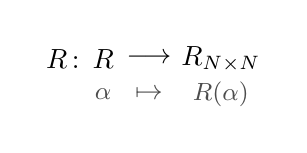
\begin{tikzpicture}[%
      baseline,
      fila2/.style={black!70,font=\small},
    ]
    \matrix (mymatrix)[row sep=-3pt, column sep=-2pt]
    {
      \node{$\mmm{R}$\,:}; & \node{$\symbb{R}$}; & \node{$\longrightarrow$}; &
      [-1pt]\node{$\mmm{R}_{N\times N}$};\\
      & \node[fila2]{$\alpha$}; & \node[black!70]{$\mapsto$}; &
      \node[fila2]{$\mmm{R}(\alpha)$};\\
  };
\end{tikzpicture}
\end{center}

Un ejemplo de grupo de Lie es el que se representa como O(N), que es el grupo de las
matrices ortogonales $N\times N$; esto es, el grupo de matrices $\mmm{A}$ de componentes
reales que cumplen
\[
  \mmm{A}^{\trasp} \mmm{A} = \mmm{I}
\]

La igualdad anterior implica que
\[
  \det(\mmm{A}) = \pm 1
\]
y es válida para el grupo de rotaciones con $\det(\mmm{A}) = +1$ y para el de
reflexiones, con $\det(\mmm{A}) = -1$, en un espacio de dimensión $N$.

\[
  O(2)
  = \{ \mmm{R}(\alpha)\ |\ \mmm{R}\text{ es matriz real } 2\times 2, \mmm{R}^\trasp
  \mmm{R} = \mmm{I},\ \det(\mmm{R}) = \pm 1\}
\]


En estas transformaciones (rotaciones y reflexiones) se conserva el módulo de los
vectores del espacio
\[
  (\vvv{x}')^{2}
  = (\mmm{A}\vvv{x})^{2}
  = (\mmm{A}\vvv{x})^{\trasp} (\mmm{A}\vvv{x})
  = \vvv{x}^{\trasp} \mmm{A}^{\trasp} \mmm{A} \vvv{x}
  = \vvv{x}^{\trasp} \mmm{I} \vvv{x}
  = \vvv{x}^{\trasp} \vvv{x}
  = \vvv{x}^{2}
\]

El grupo SO(N) es el subgrupo de matrices de O(N) con determinante unidad, esto es, el
grupo de rotaciones --sin incluir las reflexiones--.

\subsubsection{SO(2)}
El grupo de rotaciones de dimensión 2 se suele representar como SO(2):
\begin{itemize}
\item La $S$ significa que las matrices son especiales
  \[
    \det(\mmm{R}) = 1
  \]
\item La $O$, que las matrices son ortogonales
  \[
    \mmm{R}^\trasp \mmm{R} = \mmm{I}
  \]
\item El $2$ hace referencia a que se trata de un grupo de matrices $2\times 2$.
\end{itemize}
Por ejemplo, el conjunto que forma el grupo de rotaciones de dimensión 2 se puede definir
\[
  SO(2)
  = \{ \mmm{R}(\alpha)\ |\ \mmm{R}\text{ es matriz real } 2\times 2, \mmm{R}^\trasp
  \mmm{R} = \mmm{I},\ \det(\mmm{R}) = 1\}
\]
que es el grupo de matrices ortogonales $2\times 2$, que describen la rotación en el
plano real y forman un grupo de Lie.

\subsection{Matriz de rotación general}\label{sec:matriz_rotacion_general}
Tenemos las siguientes propiedades de la matriz de rotación,
ecuaciones~\eqref{eq:gli-R_ortogonal} y~\eqref{eq:gli-detRuno}
\begin{align*}
  \mmm{R}^\trasp \mmm{R} &= \mmm{I}\\
  \det(\mmm{R}) &= 1
\end{align*}
y hemos obtenido una expresión concreta cuando la dimensión es 2,
ver~\eqref{eq:gli-rotacion2x2}
\[
  \mmm{R}(\alpha)
  = \begin{pmatrix}
    \cos\alpha & \sin\alpha\\
    -\sin\alpha & \cos\alpha
    \end{pmatrix}
\]

Nos proponemos hallar la expresión general para la matriz de rotación,
independientemente de la dimensión del espacio en el que se realiza la transformación
(simplificando bastante la notación).

Supongamos que queremos rotar un sistema un ángulo finito $0 \leq \alpha < 2\pi$.
Sabemos que rotar un ángulo $\alpha$ equivale a rotar $N$ veces el ángulo $\alpha / N$.
En particular, estamos interesados en valores de $N$ muy grandes, que tienden a
infinito, es decir, valores para los que $\varepsilon=\alpha/N$ sea una cantidad
infinitesimal
\[
  \alpha = N\,\dfrac{\alpha}{N} = N \varepsilon
\]

Si un parámetro $\varepsilon$ es infinitesimal, en primera aproximación, se considera
que su cuadrado es despreciable ($\varepsilon^2\approx 0$).

Una rotación infinitesimal cambia algo el objeto rotado, pero muy poco, de manera que
casi lo deja igual. Esto se puede representar matemáticamente
\[
  \mmm{R}(\varepsilon) = \mmm{R}\left(\dfrac{\alpha}{N}\right) = \mmm{I} + \mmm{A}
\]
donde $\mmm{A}$ es una matriz infinitesimal.

La rotación finita sería el resultado de aplicar sucesivamente un número $N$ (que tiende
a infinito) de rotaciones, de manera que hay que multiplicar $\mmm{R}(\varepsilon)$ por
sí misma, $N$ veces
\[
  \mmm{R} (\alpha)
  = \underbrace{%
    \mmm{R}(\varepsilon) \mmm{R}(\varepsilon) \cdots \mmm{R}(\varepsilon)
    }_{N\text{ veces}}
  = \mmm{R}(\varepsilon)^N = (\mmm{I} + \mmm{A})^N
\]

Analicemos cómo debería ser la matriz infinitesimal $\mmm{A}$.
La matriz de rotación infinitesimal $\mmm{R}(\varepsilon) = \mmm{I} + \mmm{A}$,
por ser matriz de rotación, debe ser ortogonal
\[
  \mmm{R}^\trasp \mmm{R} = \mmm{I}
\]
\[
  (\mmm{I} + \mmm{A})^\trasp \, (\mmm{I} + \mmm{A}) = \mmm{I}
\]
\[
  (\mmm{I}^\trasp + \mmm{A}^\trasp)\, (\mmm{I} + \mmm{A}) = \mmm{I}
\]
\[
  (\mmm{I} + \mmm{A}^\trasp)\, (\mmm{I} + \mmm{A}) = \mmm{I}
\]
\[
  \mmm{I} \mmm{I}
  + \mmm{I} \mmm{A}
  + \mmm{A}^\trasp \mmm{I}
  + \mmm{A}^\trasp \mmm{A}
  = \mmm{I}
\]
\[
  \mmm{I} + \mmm{A} + \mmm{A}^\trasp + \symcal{O}\left(A^2\right) = \mmm{I}
\]

Nótese que $\mmm{A}^\trasp \mmm{A}$ es despreciable porque $\mmm{A}$ es infinitesimal.
La expresión~\eqref{eq:gli-A_antisimetrica} que se obtiene, define a la matriz \mmm{A}
como antisimétrica, $\mmm{A}^\trasp = -\mmm{A}$
\begin{equation}\label{eq:gli-A_antisimetrica}
  \mmm{A} + \mmm{A}^\trasp = 0
\end{equation}

Los elementos de las matrices antisimétricas, como $\mmm{A}$, cumplen $A_{ij} = -A_{ji}$.
Nótese que los elementos diagonales de las matrices antisimétricas deben ser cero para
que se cumpla $A_{ii} = -A_{ii}$.

Hay dos opciones para $\mmm{A}$, reflejadas en~\eqref{eq:gli-opcionesA}, cada una es la
opuesta de la otra.
En principio cualquiera sería válida.
La clave reside en el significado que le demos al ángulo de rotación $\varepsilon$.
Podría definirse como el ángulo que giran los ejes o el que giran los vectores; cada uno
de los ángulos es opuesto del otro, de ahí que las dos matrices posibles sean inversas
\begin{equation}\label{eq:gli-opcionesA}
  \mmm{A}
  =
  \begin{pmatrix}
    0 & \varepsilon\\
    -\varepsilon & 0
  \end{pmatrix}
  \hspace{1em}
  \text{o}
  \hspace{1em}
  \mmm{A}
  =
  \begin{pmatrix}
    0 & -\varepsilon\\
    \varepsilon & 0
  \end{pmatrix}
\end{equation}

Sólo tenemos un grado de libertad, $\varepsilon$.
De acuerdo con nuestro convenio de rotación pasiva (giro de los ejes de coordenadas),
definimos $\varepsilon$ como \emph{el ángulo que giran los ejes de coordenadas},
teniendo en cuenta que el sentido positivo es el antihorario.
¿Cómo podemos saber cuál de las dos matrices anteriores es la que se corresponde con
nuestro convenio?

Para dilucidarlo, hacemos girar infinitesimalmente los ejes en sentido positivo, por lo
tanto los vectores aparentarán girar en sentido negativo, tal y como se aprecia en la
figura~\ref{fig:gli-girovector}.
Ahora construimos las transformaciones que se obtienen y vemos que la coordenada $x$
aumenta ligeramente, de ahí la suma en la expresión~\eqref{eq:gli-giro_incx}; en cambio,
la coordenada $y$ disminuye ligeramente, y la ecuación~\eqref{eq:gli-giro_incy}
representa esta transformación
\begin{subequations}\label{eq:gli-giro_incxy}
  \begin{align}
    \label{eq:gli-giro_incx}
    x' &= x + \varepsilon y \\
    \label{eq:gli-giro_incy}
    y' &= y - \varepsilon x
  \end{align}
\end{subequations}

Podemos resumir de forma matricial las ecuaciones~\eqref{eq:gli-giro_incxy} anteriores
\begin{equation}\label{eq:gli-giro_incxy_matricial}
  \begin{pmatrix}
    x' \\ y'
  \end{pmatrix}
  = \begin{pmatrix}
    x + \varepsilon y\\
    y - \varepsilon y
    \end{pmatrix}
\end{equation}

\begin{figure}[ht]
  % Escala
  \def\scl{1}
  % Eje x
  \pgfmathsetmacro{\XMLONG}{0}
  \pgfmathsetmacro{\XPLONG}{3}
  % Eje y
  \pgfmathsetmacro{\YMLONG}{0}
  \pgfmathsetmacro{\YPLONG}{3}
  % Ángulo rotado
  \pgfmathsetmacro{\ANGROT}{20}
  % Vector P
  \pgfmathsetmacro{\PMOD}{2.5}
  \pgfmathsetmacro{\PANG}{60}
  % Vector P'
  \pgfmathsetmacro{\PPRIMAMOD}{\PMOD}
  \pgfmathsetmacro{\PPRIMAANG}{\PANG - \ANGROT}
  % Fondo
  \pgfmathsetmacro{\HORZ}{0.23}
  \pgfmathsetmacro{\VERT}{0.25}
  \pgfmathsetmacro{\MOD}{sqrt(\HORZ^2 + \VERT^2)}
  \pgfmathsetmacro{\ANGSD}{atan(\VERT / \HORZ)}
  \pgfmathsetmacro{\ANGII}{\ANGSD + 180.0}
  % 
  \centering
  \begin{tikzpicture}[%
    scale=\scl,
    every node/.style={black,font=\small},
    eje/.style={->},
    vector/.style={-{Latex}, shorten >=1.2pt, line width=.8pt},
    vectorrotado/.style={vector, draw=green!50!black},
    pcirculo/.style={fill=red, draw=black},
    pprimacirculo/.style={green!90!black, draw=black},
    background/.style={
      line width=\bgborderwidth,
      draw=\bgbordercolor,
      fill=\bgcolor,
    },
    ]
    % Coordenadas
    \coordinate (O) at (0,0);
    \coordinate (under_origin) at (0,-3mm);
    \coordinate (left_origin) at (-3mm,0);
    \coordinate (xini) at (-\XMLONG cm,0);
    \coordinate (xfin) at (\XPLONG cm,0);
    \coordinate (yini) at (0,-\YMLONG cm);
    \coordinate (yfin) at (0,\YPLONG cm);
    \coordinate (P) at (\PANG:\PMOD cm);
    \coordinate (P') at  (\PPRIMAANG:\PPRIMAMOD);
    \path (O) -- coordinate (OPmidway) (P);
    \path (O) -- coordinate (OP'midway) (P');
    \path (O) -- coordinate[pos=1.2] (parrow) (P);
    \path (O) -- coordinate[pos=1.2] (p'arrow) (P');
    % Ángulo \varepsilon
    \path (P') -- (O) -- (P) pic
    [draw=black!50!,fill=green!20,"\footnotesize $\varepsilon$",angle
    radius=6mm, angle eccentricity=1.5] {angle = P'--O--P};
    % Ejes
    \draw[eje] (xini) -- (xfin);
    \node[right, name=letraejex] at (xfin) {$x$};
    \draw[eje] (yini) -- (yfin);
    \node[above, name=letraejey] at (yfin) {$y$};
    % Punto P
    \draw[vector] (O) -- (P);
    \node[above=5pt] at (OPmidway) {$\vvv{r}$};
    \fill[pcirculo] (P) circle [radius=1.4pt];
    \node[above] at (P) {$P$};
    % Punto P'
    \draw[vectorrotado] (O) -- (P');
    \node[right=0pt] at (OP'midway) {$\vvv{r}'$};
    \fill[pprimacirculo] (P') circle [radius=1.4pt];
    \node[right] at (P') {$P'$};
    % Sentido de giro del vector
    \draw [-{Latex},green!40!black,shorten <= 3pt]
    (parrow) to[bend left=30] (p'arrow);
    % Incremento x
    \draw[fill=red,draw=black] (P |- O) circle[radius=1.5pt];
    \draw[fill=green!80!black,draw=black] (P' |- O)
    circle[radius=1.5pt];
    \draw[-{Latex}] (P |- under_origin) --
    node[below,name=incx] {\scriptsize $\Delta x > 0$} (P' |- under_origin);
    % Incremento y
    \draw[fill=red,draw=black] (P -| O) circle[radius=1.5pt];
    \draw[fill=green!80!black,draw=black] (P' -| O)
    circle[radius=1.5pt];
    \draw[-{Latex}] (P -| left_origin) --
    node[above=-1pt,sloped,rotate=180,name=incy]
    {\scriptsize $\Delta y < 0$} (P' -| left_origin);
    % Origen
    \filldraw (O) circle [radius=.2pt];
      % Fondo amarillo
      \path (current bounding box.south west) ++(\ANGII:\MOD) coordinate (SW);
      \path (current bounding box.north east) ++(\ANGSD:\MOD) coordinate (NE);
      % \filldraw[draw=black, fill=red] (NE) circle[radius=1pt];
      \begin{scope}[on background layer]
        \draw[background] (SW) rectangle (NE);
      \end{scope}    
%    \begin{scope}[on background layer]
%      \node [background, fit= (incx) (incy) (letraejex) (letraejey)] {};
%    \end{scope}
  \end{tikzpicture}
  \caption{Giro infinitesimal antihorario $\varepsilon$, de los ejes
    $x$ e $y$, que desde el punto de vista de estos, el vector aparenta
    girar en sentido contrario horario.}
  \label{fig:gli-girovector}
\end{figure}

Como no sabemos cuál de las dos matrices~\eqref{eq:gli-opcionesA} es la correcta para
nuestra definición de ángulo girado, la representaremos por
\[
  \mmm{A}(\varepsilon)
  = \begin{pmatrix}
    0 & a_{12}\\
    a_{21} & 0
    \end{pmatrix}
\]
Por otro lado, el vector girado $\vvv{x}'$ se puede obtener aplicando la matriz de
rotación infinitesimal desconocida al vector original $\vvv{x}$
\[
  \vvv{x}'
  =
  \mmm{R}(\varepsilon)\vvv{x}
  =
  \left[\mmm{I}+\mmm{A}(\varepsilon)\right]\vvv{x}
\]
\[
  \begin{pmatrix} x' \\ y'\end{pmatrix}
  =
  \left[
    \begin{pmatrix}
      1 & 0\\
      0 & 1
    \end{pmatrix}
    + \begin{pmatrix}
      0 & a_{12}\\
      a_{21} & 0
    \end{pmatrix}
  \right]
  \begin{pmatrix}x \\ y \end{pmatrix}           
  = \begin{pmatrix}
    x \\ y
  \end{pmatrix}
  + \
  \begin{pmatrix}
    a_{12}y \\ a_{21}x
  \end{pmatrix}\\
  =
  \begin{pmatrix}
    x + a_{12}y\\
    y + a_{21}x
  \end{pmatrix}
\]

Si comparamos este resultado con la igualdad~\eqref{eq:gli-giro_incxy_matricial},
llegamos a la conclusión de que
\begin{align*}
  a_{12} &= \varepsilon\\
  a_{21} &= -\varepsilon
\end{align*}
 
Así, la matriz que buscamos es
 \[
   \mmm{A}
   =
   \begin{pmatrix}
     0 & \varepsilon\\
     -\varepsilon & 0
   \end{pmatrix}
 \]

\subsection{Generador de una rotación pasiva}
Extrayendo el ángulo $\varepsilon$ de la matriz, obtenemos
\[
  \mmm{A}
  =
  \begin{pmatrix}
    0 & \varepsilon \\
    -\varepsilon & 0
  \end{pmatrix}
  = \varepsilon
  \begin{pmatrix}
    0 & 1\\
    -1 & 0
  \end{pmatrix}
  = \varepsilon\mmm{G}
\]
recordemos $\varepsilon=\alpha/N$ es un infinitésimo.

$\mmm{G}$ se denomina \emph{generador de la rotación} y
también es una matriz antisimétrica.
\begin{equation}
  \mmm{G}
  =
  \begin{pmatrix}
    0 & 1\\
    -1 & 0
  \end{pmatrix}
\end{equation}

La matriz de rotación infinitesimal queda
\[
  \mmm{R} (\varepsilon) = \mmm{I} + \varepsilon\mmm{G}
\]

La matriz genérica de rotación sería
\[
  \mmm{R} (\alpha) = (\mmm{I} + \varepsilon\mmm{G})^N
\]
\begin{equation}
  \label{eq:gli-matriz_rotacion_N}
  \mmm{R} (\alpha) = \left(\mmm{I} + \dfrac{\alpha}{N}\,\mmm{G}\right)^N
\end{equation}

Queremos obtener un desarrollo en serie de potencias de $\alpha$ de la
expresión~\eqref{eq:gli-matriz_rotacion_N}, alrededor de $\alpha = \SI{0}{\radian}$,
calculando los valores de la matriz de rotación y algunas de sus sucesivas derivadas
para el ángulo de cero radianes, teniendo en cuenta que $N$ tiende a infinito
\begin{equation}\label{eq:gli-desarrolloserie_R}
  \mmm{R} (\alpha)
  = \mmm{R} (0)
  + \mmm{R}'(0)\,\alpha
  + \dfrac{1}{2!}\,\mmm{R}'' (0)\,\alpha^2
  + \dfrac{1}{3!}\,\mmm{R}''' (0)\,\alpha^3
  + \dfrac{1}{4!}\,\mmm{R}^{IV} (0)\,\alpha^4
  + \cdots
\end{equation}

A continuación calculamos las derivadas de $\mmm{R(\alpha)}$ en $alpha = 0$:
\begin{itemize}
\item La matriz sin derivar y su valor en $\varepsilon=\alpha/N = 0$ son,
  respectivamente
\[
  \mmm{R} (\alpha) = \left(\mmm{I} + \dfrac{\alpha}{N}\,\mmm{G}\right)^N
  ;\hspace{1em}
  \mmm{R} (0) = \mmm{I}^N = \mmm{I}
\]

\item La primera derivada con respecto de $\alpha$ y su valor en $\varepsilon=\alpha/N=0$
\[
  \mmm{R}' (\alpha)
  = N\,\dfrac{\mmm{G}}{N}\,\left(\mmm{I} +
    \dfrac{\alpha}{N}\,\mmm{G}\right)^{N-1}
  ;\hspace{1em} \mmm{R}' (0) = \mmm{G}\, \mmm{I}^{N-1} = \mmm{G}
\]

\item La segunda derivada
\[
  \mmm{R}'' (\alpha) = N\,(N-1)\,\dfrac{\mmm{G}^2}{N^2}\,\left(\mmm{I} +
    \dfrac{\alpha}{N}\,\mmm{G}\right)^{N-2}
  ;\hspace{1em} \mmm{R}'' (0) = \dfrac{N\,(N-1)\,\mmm{G}^2}{N^2} = \mmm{G}^2
\]

Nótese que $N\,(N-1)/N^2\to 1$ cuando $N\to \infty$, que es la condición que imponíamos a $N$.

\item Obtenemos una derivada más y su valor en $\varepsilon=0$
{\small
\[
  \mmm{R}''' (\alpha) = N\,(N-1)\,(N-2)\,\dfrac{\mmm{G}^3}{N^3}\,\left(\mmm{I} +
    \dfrac{\alpha}{N}\,\mmm{G}\right)^{N-3}
  ;\hspace{1em} \mmm{R}''' (0) = \dfrac{N\,(N-1)\,(N-2)\,\mmm{G}^3}{N^3}
  = \mmm{G}^3
\]
}
y así sucesivamente.

\item Generalizando, la derivada n-ésima en $\alpha=0$ es
\[
  \mmm{R}^{(n)}(0) = \mmm{G}^n
\]
\end{itemize}

Desarrollamos la matriz de rotaciones en serie de potencias de $\alpha$
\eqref{eq:gli-desarrolloserie_R}, teniendo en cuenta los cálculos previos
\begin{equation}\label{eq:gli-desarrolloserie_G}
  \mmm{R} (\alpha)
  = \mmm{I}
  + \mmm{G}\,\alpha
  + \dfrac{1}{2!}\,\mmm{G}^2 \alpha^2
  + \dfrac{1}{3!}\,\mmm{G}^3 \alpha^3
  + \dfrac{1}{4!}\,\mmm{G}^4 \alpha^4
  + \cdots
\end{equation}

La forma general de una matriz de rotación queda
{\large
\begin{equation}\label{eq:gli-rotgeneral}
  \mmm{R} (\alpha) = e^{\alpha\mmm{G}}
\end{equation}
}
donde $\alpha$ es el ángulo que giran los ejes de coordenadas y
$\mmm{G}$ es una matriz antisimétrica.

Si $\alpha$ representara el ángulo que giran los vectores, entonces
el ángulo de rotación pasiva sería el opuesto, $-\alpha$
{\large
\begin{equation}\label{eq:gli-rotobjgeneral}
  \mmm{R} (\alpha) = e^{-\alpha\mmm{G}}
\end{equation}
}

\subsection{Obtención de la matriz de rotación en
  \mathinhead{\symbb{R}^2}{OdlamdreR2}}
Para terminar esta sección, vamos a comprobar que la expresión anterior es
correcta, volviendo a obtener la matriz de rotación en dos dimensiones,
que ya dedujimos en la ecuación~\eqref{eq:gli-matriz_rotacion_2x2},
desarrollando la fórmula general en la ecuación~\eqref{eq:gli-rotgeneral}.

Las únicas matrices antisimétricas $2\times 2$ son
\begin{equation}\label{eq:gli-g_so2}
  \mmm{G} =
  \begin{pmatrix}
    0 & 1\\
    -1 & 0
  \end{pmatrix}
\end{equation}
y su inversa, que no es independiente de la anterior; de manera que
tomamos la primera como generadora de la rotación SO(2).

Calculamos algunas potencias de $\mmm{G}$ ahorrándonos los detalles
\begin{align*}
  \mmm{G}^2 &= -\mmm{I}\\
  \mmm{G}^3 &= -\mmm{G}\\
  \mmm{G}^4 &= \mmm{I}\\
  \mmm{G}^5 &= \mmm{G}\\
  &\cdots
\end{align*}

Entonces, el desarrollo en serie~\eqref{eq:gli-desarrolloserie_G}:
\begin{align*}
  \mmm{R} (\alpha) &= e^{\alpha\mmm{G}}
   = \mmm{I} + \mmm{G}\kern1pt\alpha+ \dfrac{1}{2!}\,\mmm{G}^2 \alpha^2
             + \dfrac{1}{3!}\,\mmm{G}^3 \alpha^3
             + \dfrac{1}{4!}\,\mmm{G}^4 \alpha^4 + \cdots\\
  &= \mmm{I} + \mmm{G}\kern1pt\alpha + \dfrac{1}{2!}\,(-\mmm{I})^2\,\alpha^2
    + \dfrac{1}{3!}\,(-\mmm{G})^3 \alpha^3+ \dfrac{1}{4!}\,\mmm{I}^4 \alpha^4
    + \cdots\\
  &= \mmm{I} + \alpha\mmm{G} + \dfrac{1}{2!}\,\alpha^{2}\,\mmm{I}
    - \dfrac{1}{3!}\,\alpha^{3}\,\mmm{G}+ \dfrac{1}{4!}\,\alpha^4\,\mmm{I}
    + \cdots\\
  &=
    \left(
    1+\frac{1}{2!}\,\alpha^{2}+\frac{1}{4!}\,\alpha^{4}+\cdots
    \right)\,\mmm{I}
    + \left(
    \alpha+\frac{1}{3!}\,\alpha^{3}+\frac{1}{5!}\,\alpha^{5}+\cdots
    \right)\,\mmm{G}\\
  &=
    \cos\alpha\,\mmm{I} + \sin\alpha\,\mmm{G}
   =
    \cos\alpha\,\begin{pmatrix}1 & 0\\ 0 & 1\end{pmatrix}
   + \sin\alpha\,\begin{pmatrix}0 & 1\\ -1 & 0\end{pmatrix}\\
  &=
    \begin{pmatrix}\cos\alpha & 0\\ 0 & \cos\alpha\end{pmatrix}
    + \begin{pmatrix}0 & \sin\alpha\\ -\sin\alpha & 0\end{pmatrix}
  =
 \begin{pmatrix}\cos\alpha & \sin\alpha\\ -\sin\alpha & \cos\alpha\end{pmatrix}
\end{align*}

obteniéndose el resultado esperado \eqref{eq:gli-rotacion2x2}.


%%% Local Variables:
%%% mode: latex
%%% TeX-engine: luatex
%%% TeX-master: "../gruposlie.tex"
%%% End:

% lorentz.tex
%
% Copyright (C) 2022--2025 José A. Navarro Ramón <janr.devel@gmail.com>
% Licencia del código GPLv2
% Licencia Creative Commons Recognition Non-Commercial Share-alike.
% (CC-BY-NC-SA)

\chapter{El grupo de Lorentz}
En este capítulo vamos a analizar una transformación, que no es exactamente una rotación
---al menos no una rotación ordinaria en el espacio euclídeo---.

En el capítulo anterior obtuvimos la expresión general ~(\ref{eq:gli-rotgeneral}) para
una matriz de rotación pasiva
\[
  \mmm{R} (\alpha) = e^{\alpha\mmm{G}}
\]

Recordemos que $\alpha$ es el ángulo girado y $\mmm{G}$ es el generador de la rotación
---una matriz antisimétrica---. Esto último venía impuesto porque se debía cumplir que
la matriz de rotación tenía que ser ortogonal, $\mmm{R}^\trasp \mmm{R} = \mmm{I}$.
Además, el determinante de la matriz de rotación tenía que valer 1, $\det(\mmm{R}) = 1$.
Vimos la matriz de rotación pasiva en dos dimensiones
\[
  \mmm{R} (\alpha)
  = e^{\alpha\mmm{G}}
  = e^{\alpha\,{\scriptscriptstyle
      \begin{pmatrix} 0 & 1 \\ -1 & 0\end{pmatrix}}}
  =
  \begin{pmatrix}
    \cos\alpha & \sin\alpha\\
    -\sin\alpha & \cos\alpha
  \end{pmatrix}
\]

Se puede comprobar que el generador de esta rotación en dos dimensiones es una matriz
antisimétrica
\[
  \mmm{G} = \begin{pmatrix} 0 & 1 \\ -1 & 0\end{pmatrix}
\]

\section{Generador simétrico}
Ahora nos podríamos preguntar qué pasaría si el generador fuera una matriz simétrica,
por ejemplo
\[
  \mmm{G} = \begin{pmatrix} 0 & 1 \\ 1 & 0\end{pmatrix}
\]

Está claro que el generador ya no puede ser el de una rotación. Nuestro objetivo será
obtener la matriz de transformación en dos dimensiones de forma explícita, que por no
ser una rotación la representaremos por $\mmm{\Lambda} (\alpha)$
\begin{equation}\label{eq:lor-lambdarotexp}
  \mmm{\Lambda} (\alpha)
  = e^{\alpha\,{\scriptscriptstyle \begin{pmatrix} 0 & 1 \\ 1 & 0\end{pmatrix}}}
\end{equation}

Desarrollamos la exponencial en serie de potencias
\[
  \mmm{\Lambda} (\alpha)
  =
  \mmm{I} + \mmm{G}\kern1pt\alpha + \dfrac{\mmm{G}^2}{2!}\,\alpha^2
  + \dfrac{\mmm{G}^3}{3!}\,\alpha^3 + \dfrac{\mmm{G}^4}{4!}\,\alpha^4
  + \dfrac{\mmm{G}^5}{5!}\,\alpha^5 
  + \cdots
\]

Presentamos las potencias de la matriz generadora, sin mostrar todos los detalles
\begin{align*}
  \mmm{G}^2 &=  \mmm{I}\\
  \mmm{G}^3 &= \mmm{G}^2\,\mmm{G} = \mmm{I}\kern1pt\mmm{G} = \mmm{G}\\
  \mmm{G}^4 &= \mmm{G}^2\,\mmm{G}^2 = \mmm{I}\kern1pt\mmm{I} = \mmm{I}\\
  \cdots &
\end{align*}

Sustituimos estas potencias en el desarrollo de la matriz de transformación
\begin{align*}
  \mmm{\Lambda} (\alpha)
  &=
    \mmm{I} + \mmm{G}\kern1pt\alpha + \dfrac{\mmm{I}}{2!}\,\alpha^2
    + \dfrac{\mmm{G}}{3!}\,\alpha^3 + \dfrac{\mmm{I}}{4!}\,\alpha^4
    + \dfrac{\mmm{G}}{5!}\,\alpha^5 + \dfrac{\mmm{I}}{6!}\,\alpha^6
    + \cdots\\
  &= \mmm{I} + \dfrac{\mmm{I}}{2!}\,\alpha^2 + \dfrac{\mmm{I}}{4!}\,\alpha^4
    + \cdots
    + \mmm{G}\kern1pt\alpha  + \dfrac{\mmm{G}}{3!}\,\alpha^3
    + \dfrac{\mmm{G}}{5!}\,\alpha^5
    + \cdots\\
  &= \left(1 + \dfrac{1}{2!}\,\alpha^2 + \dfrac{1}{4!}\,\alpha^4
    +\cdots\right) \mmm{I}
    + \left(\alpha + \dfrac{1}{3!}\,\alpha^3 + \dfrac{1}{5!}\,\alpha^5
    +\cdots\right) \mmm{B}\\
  &= \cosh\alpha\,\mmm{I} + \sinh\alpha\,\mmm{G}\\
  &= \cosh\alpha\,\begin{pmatrix}1 & 0 \\ 0 & 1 \end{pmatrix}
    + \sinh\alpha\,\begin{pmatrix} 0 & 1 \\ 1 & 0 \end{pmatrix}\\
    \end{align*}

\section{Transformación de Lorentz}
La matriz de transformación en dos dimensiones anterior la podemos compactar
\begin{equation}\label{eq:lor-lambdarotmatriz}
  \mmm{\Lambda} (\alpha)
  =
  \begin{pmatrix}
    \cosh\alpha & \sinh\alpha \\ \sinh\alpha & \cosh\alpha
  \end{pmatrix}
\end{equation}

Esta matriz es la que representa la transformación de Lorentz, que es fundamental en
relatividad.
Para seguir la costumbre en relatividad, las componentes de los vectores de Lorentz
las representaremos con un superíndice. Más tarde se verá el motivo.

\subsection{Determinante e inversa de la transformación de Lorentz}
Tal y como ocurría con la rotación en el espacio euclídeo, el determinante de la matriz
de transformación de Lorentz también vale 1
\[
  \det(\mmm{\Lambda})
  = \begin{vmatrix}
    \cosh\alpha \sinh\alpha\\
    \sinh\alpha \cosh\alpha
  \end{vmatrix}
  = \cosh^2\alpha - \sinh^2\alpha
  = 1
\]

Pero, al contrario que ocurría con la rotación en el espacio euclídeo, esta matriz
inversa no es la transpuesta de la matriz de transformación
$\mmm{\Lambda}^{-1} \neq \mmm{\Lambda}^{\trasp}$, y por tanto, la matriz de transformación
de Lorentz no es ortogonal
\[
  \mmm{\Lambda}^{\trasp} \mmm{\Lambda} \neq \mmm{I}
\]

\subsection{Invariante de la transformación}
Ahora estamos interesados en buscar si esta transformación tiene algún invariante
\[
  \vvv{x'} = \mmm{\Lambda} \, \vvv{x}
\]
\[
  \begin{pmatrix}
    x'^0 \\ x'^1
  \end{pmatrix}
  =
  \begin{pmatrix}
    \cosh\alpha & \sinh\alpha \\ \sinh\alpha & \cosh\alpha
  \end{pmatrix}
  \,
  \begin{pmatrix}
    x^0 \\ x^1
  \end{pmatrix}
\]

\begin{align*}
  x'^0 &= x^0 \cosh\alpha + x^1 \sinh\alpha\\
  x'^1 &= x^0 \sinh\alpha + x^1 \cosh\alpha
\end{align*}

Elevamos al cuadrado cada ecuación
\begin{align*}
  (x'^0)^2 &= \left(x^0 \cosh\alpha + x^1 \sinh\alpha\right)^2\\
  &= (x^0)^2\cosh^2\alpha + (x^1)^2\sinh^2\alpha + 2x^0x^1\sinh\alpha\,\cosh\alpha
\end{align*}
\begin{align*}
  (x'^1)^2 &= \left(x^0\sinh\alpha + x^1\cosh\alpha\right)^2\\
           &= (x^0)^2\sinh^2\alpha + (x^1)^2\cosh^2\alpha
             + 2x^0x^1\sinh\alpha\,\cosh\alpha
\end{align*}

Si sumáramos las ecuaciones no encontraríamos ningún invariante; en lugar de ello las restamos y tenemos en cuenta que $\cosh^2\alpha - \sinh^2\alpha = 1$
\begin{align*}
  (x'^0)^2 - (x'^1)^2
  &= (x^0)^2 (\cosh^2\alpha - \sinh^2\alpha)
    + (x^1)^2 (\sinh^2\alpha - \cosh^2\alpha)
  = (x^0)^2 - (x^1)^2
\end{align*}

Entonces el invariante resulta ser
\begin{equation}\label{eq:lor-invariante}
  (x'^0)^2 - (x'^1)^2 = (x^0)^2 - (x^1)^2 = \text{constante}
\end{equation}

\subsection{Métrica}
Hemos representado el invariante de la transformación de Lorentz a través de las
componentes. Ahora tenemos que conseguirlo sin ellas.
Para ello, analizamos el cuadrado de $\vvv{x}$ y comprobamos que no da el invariante de
la transformación de Lorentz
\[
  \vvv{x}^2 = \vvv{x}^\trasp\,\vvv{x}
  = \begin{pmatrix}
    x^0 & x^1
  \end{pmatrix}
  \,
  \begin{pmatrix}
    x^0 \\ x^1
  \end{pmatrix}
  = (x^0)^2 + (x^1)^2
  \neq
  (x^0)^2 - (x^1)^2
\]

Pero, nos interesa generalizar el concepto de producto escalar para que sirva,
tanto para los vectores de rotación como para los vectores de Lorentz.
Lo haremos añadiendo el concepto de \emph{métrica}, que nos sirve para definir cómo
podemos medir longitudes --y en su caso, intervalos temporales-- en el espacio que
nos interese.

El producto escalar de dos vectores $x$ e $y$ en forma matricial se define como
\[
  \vvv{x}\cdot \vvv{y} = \vvv{x}^\trasp\mmmg{\eta}\kern1pt\vvv{y}
\]
donde $\mmmg{\eta}$ es una matriz cuadrada que denominamos \emph{métrica}.

Veamos un ejemplo con vectores de rotación; en este caso la métrica es la matriz
identidad, y por ejemplo, el cuadrado de un vector funciona como se espera
\[
  \vvv{x}^2
  = \vvv{x}\cdot \vvv{x}
  = \vvv{x}^\trasp \mmmg{\eta}\kern1pt\vvv{x}
  = \vvv{x}^\trasp \kern1pt\mmm{I}\,\vvv{x} = \vvv{x}^\trasp \vvv{x}
\]
\[
  \vvv{x}^2 
  = \begin{pmatrix}
    x_1 & x_2
  \end{pmatrix}
  \,
  \begin{pmatrix}
    1 & 0 \\ 0 & 1
  \end{pmatrix}
  \,
  \begin{pmatrix}
    x_1 \\ x_2
  \end{pmatrix}
  =
  \begin{pmatrix}
    x_1 & x_2
  \end{pmatrix}
  \,
  \begin{pmatrix}
    x_1 \\ x_2
  \end{pmatrix}
  = x_1^2 + x_2^2
\]

El cuadrado de un vector de Lorentz será, con la métrica apropiada y en dos dimensiones
\begin{align*}
  \vvv{x}^2
  &= \vvv{x}\cdot \vvv{x}
    = \vvv{x}^\trasp \mmmg{\eta}\,\vvv{x}
  =
  \begin{pmatrix}
    x^0 & x^1
  \end{pmatrix}
  \,
  \begin{pmatrix}
    1 & 0 \\ 0 & -1
  \end{pmatrix}
  \,
  \begin{pmatrix}
    x^0 \\ x^1
  \end{pmatrix}
  =
  \begin{pmatrix}
    x^0 & x^1
  \end{pmatrix}
  \,
  \begin{pmatrix}
    x^0 \\ -x^1
  \end{pmatrix}\\
  &= (x^0)^2 - (x^1)^2
\end{align*}

Ahora bien, la teoría de la relatividad contempla cuatro dimensiones y los vectores se
denominan cuadrivectores
\[
  \begin{pmatrix}
    x^0 \\ x^1 \\ x^2 \\ x^3
  \end{pmatrix}
\]

La primera, $x^0$, es una componente temporal, a menudo se escribe $ct$, y las demás,
$x^1$, $x^2$ y $x^3$, son las tres componentes espaciales, que a veces representamos
como $x$, $y$ y $z$.

La métrica en cuatro dimensiones debe cambiar el signo de las componentes espaciales y
dejar inalterada la componente temporal
\[
  \mmmg{\eta}\kern1pt\vvv{x} =
  \begin{pmatrix}
    1 & 0 & 0 & 0\\
    0 & -1 & 0 & 0\\
    0 & 0 & -1 & 0\\
    0 & 0 & 0 & -1
  \end{pmatrix}
  \,
  \begin{pmatrix}
    x^0 \\ x^1 \\ x^2 \\ x^3
  \end{pmatrix}
  =
  \begin{pmatrix}
    x^0 \\ -x^1 \\ -x^2 \\ -x^3
  \end{pmatrix}
  =
  \begin{pmatrix}
    x_0 \\ x_1 \\ x_2 \\ x_3
  \end{pmatrix}
\]
En la subsección que sigue se dará una idea somera de qué significa el cambio de
superíndices por subíndices en el vector resultante de operar la métrica con un
vector de Lorentz.

Esta métrica, en relatividad especial, se denomina \emph{métrica de Minkowski}
($\eta_{\mu\nu}$), y define la geometría plana del espacio-tiempo de cuatro dimensiones
y la invariancia de la distancia propia (intervalo espacio-temporal).

\subsection{Vector dual}
El vector obtenido en la operación anterior se llama \emph{vector dual de }$\vvv{x}$.
Decimos que el vector dual de uno dado es el resultado de operar la métrica con el
vector. Así, para hallar el vector dual del vector de Lorentz $\vvv{x}$ en dos
dimensiones
\[
  \mmmg{\eta}\kern1pt\vvv{x} =
  \begin{pmatrix} 1 & 0 \\ 0 & -1 \end{pmatrix} \,
  \begin{pmatrix}x^0 \\x^1 \end{pmatrix} =
  \begin{pmatrix}x^0 \\ -x^1 \end{pmatrix} =
  \begin{pmatrix}x_0 \\ x_1 \end{pmatrix}
\]

Como se puede observar en la igualdad anterior, en la práctica, en lugar de tomarnos la
molestia de cambiar el signo o valor de algunas componentes al operar la métrica con un
vector de Lorentz, lo que hacemos es cambiar de sitio el subíndice o superíndice de
manera que, si está como superíndice lo convertimos en subíndice y viceversa.
\[
  \mmmg{\eta}
  \begin{pmatrix}
    x^0 \\ x^1
  \end{pmatrix}
  =
  \begin{pmatrix}x_0 \\ x_1 \end{pmatrix}
\]

Sólo hay que tener la precaución de que cuando se realice el cambio, habría que cambiar
el signo de las componentes espaciales y mantener el de la componente temporal en el
caso de métrica y vectores de Lorentz
\[
  x_0 = x^0 ;\hspace{1em} x_1 = -x^1
\]

El invariante de Lorentz se podrá escribir ahora como
\begin{align*}
  (\vvv{x'})^2 &= \vvv{x}^\trasp \mmmg{\eta}\kern1pt\vvv{x}
  =
  \begin{pmatrix}
    x^0 & x^1
  \end{pmatrix}
  \,
  \begin{pmatrix}
    1 & 0 \\ 0 & -1
  \end{pmatrix}
  \,
  \begin{pmatrix}
    x^0 \\ x^1
  \end{pmatrix}
  =
  \begin{pmatrix}
    x^0 & x^1
  \end{pmatrix}
  \,
  \begin{pmatrix}
    x^0 \\ -x^1
  \end{pmatrix}\\
  &=
  \begin{pmatrix}
    x^0 & x^1
  \end{pmatrix}
  \,
  \begin{pmatrix}
    x_0 \\ x_1
  \end{pmatrix}
  = x^0 x_0 + x^1 x_1
  = x_0 x^0 + x_1 x^1
  = x_\mu x^\mu
\end{align*}
  
En la última expresión se ha utilizado el criterio de la suma de Einstein. Utilizamos
letras griegas para el índice cuando implica componentes temporales y espaciales; si
sólo estuvieran implicadas componentes espaciales, se usarían las típicas, $i$, $j$,
$k$, etc.



 
%%% Local Variables:
%%% mode: latex
%%% TeX-engine: luatex
%%% TeX-master: "../gruposlie.tex"
%%% End:

% so3.tex
%
% Copyright (C) 2022--2025 José A. Navarro Ramón <janr.devel@gmail.com>
% Licencia Creative Commons Recognition Share-alike.
% (CC-BY-SA)

\chapter{El grupo de rotaciones SO(3)}
En este capítulo estudiaremos el grupo de rotaciones en el espacio tridimensional.
Partimos de la expresión exponencial de la matriz de  rotación de los ejes $x$ e $y$ en
dos dimensiones en sentido antihorario
 \[
   \mmm{R} (\theta)
   = e^{\theta\mmm{G}}
   = \exp\left\{\theta\,\begin{pmatrix} 0 & 1 \\ -1 & 0 \end{pmatrix}\right\}
 \]
 siendo $\mmm{G}$ el único generador de rotación en el grupo SO(2).
 
\subsection{Número de generadores del grupo SO(3)}\label{subsec:num_gen_so3}
Para saber cuántos generadores encontraremos en el grupo SO(3), nos debemos fijar en la
expresión exponencial de una rotación en el espacio tridimensional
\[
  \mmm{R} = e^{\mmm{A}} = \exp\left\{
    \begin{pmatrix}
      A_{11} & A_{12} & A_{13}\\ A_{21} & A_{22} & A_{23}\\ A_{31} &
      A_{32} & A_{33}
    \end{pmatrix}\right\}
\]

Sabemos que la matriz $\mmm{A}$ debe ser antisimétrica:
\begin{itemize}
\item Los elementos diagonales deben ser cero, $A_{ii} = 0$
\[
    \mmm{A} =
    \begin{pmatrix}
      0 & A_{12} & A_{13}\\
      A_{21} & 0 & A_{23}\\
      A_{31} & A_{32} & 0
    \end{pmatrix}
\]

\item Los elementos que están fuera de la diagonal deben cumplir
  $A_{ij} = -A_{ji}$
  \[
    \mmm{A} =
    \begin{pmatrix}
      0 & A_{12} & A_{13}\\
      -A_{12} & 0 & A_{23}\\
      -A_{13} & -A_{23} & 0
    \end{pmatrix}
\]
\end{itemize}

Vemos que sólo tenemos tres grados de libertad: $A_{12}$, $A_{13}$ y
$A_{23}$, los demás elementos quedan completamente especificados.
Este grupo tendrá tres generadores.

Dejamos, como ejercicio, comprobar que una rotación en el plano --SO(2)-- tiene un único
generador, mientras que una rotación en el espacio de cuatro dimensiones --SO(4)--, tiene
seis.

\subsection{Generador para la rotación alrededor del eje
  \mathinhead{z}{z}, \mathinhead{\mmm{G}_z}{Gz}}
Esta rotación pasiva hace girar los ejes $x$ e $y$ de forma similar a como hemos visto
en la SO(2), así que la podemos relacionar con una rotación alrededor del eje $z$ en
tres dimensiones
\[
  \mmm{R}_z (\theta) = \exp\left\{\theta\,\begin{pmatrix} 0 & 1 \\ -1
      & 0 \end{pmatrix}\right\}
\]

Pero el generador debe ser una matriz $3\times 3$, por lo que se debe completar.
Como la matriz debe ser antisimétrica, los elementos diagonales deben ser cero
\[
  \mmm{R}_z (\theta) = \exp\left\{ \theta\,
    \begin{pmatrix}
      0 & 1 \\ -1
      & 0 \\ & & 0
    \end{pmatrix} \right\}
\]

Completamos con ceros el resto de elementos
\[
  \mmm{R}_z (\theta) = \exp\left\{ \theta\,
    \begin{pmatrix}
      0 & 1 & 0 \\ -1 & 0 & 0\\ 0 & 0 & 0
    \end{pmatrix}\right\}
\]
y el generador para la rotación pasiva alrededor del eje $z$ sería
\begin{equation}\label{eq:so3-generador_z}
  \mmm{G}_z =
  \begin{pmatrix} 0 & 1 & 0
    \\ -1 & 0 & 0\\ 0 & 0 & 0
  \end{pmatrix}
\end{equation}

Debido a la forma un poco arbitraria con que hemos obtenido este generador, tenemos que
comprobar que describe efectivamente una rotación alrededor del eje $z$.
Lo más sencillo es comprobarlo mediante una rotación infinitesimal, porque la matriz de
rotación es más sencilla, dado que los términos que contienen $\varepsilon^n$ con $n>=2$
son despreciables
\begin{equation}
  \label{eq:so3-rotacion_infinitesimal_z}
  \mmm{R}_z (\varepsilon) \approx
  \mmm{I} + \varepsilon\, \mmm{G}_z
  = \begin{pmatrix}
    1 & 0 & 0\\
    0 & 1 & 0\\
    0 & 0 & 1
  \end{pmatrix}
  + \varepsilon
  \begin{pmatrix}
    0 & 1 & 0 \\ -1 & 0 & 0\\ 0 & 0 & 0
  \end{pmatrix}
\end{equation}

Aplicamos esta pequeña rotación pasiva alrededor del eje $z$ a un
vector cualquiera del espacio de tres dimensiones
{
  \small
  \begin{align*}
   \begin{pmatrix}
     x' \\ y' \\ z'
   \end{pmatrix}
   &= \mmm{R}_z (\varepsilon)
   \begin{pmatrix}
     x \\ y \\ z
   \end{pmatrix}
   \approx
   \left[
   \begin{pmatrix}
     1 & 0 & 0\\
     0 & 1 & 0\\
     0 & 0 & 1
   \end{pmatrix}
   + \varepsilon
   \begin{pmatrix}
     0 & 1 & 0 \\ -1 & 0 & 0\\ 0 & 0 & 0
   \end{pmatrix}
  \right]\,
  \begin{pmatrix}
    x \\ y \\ z
  \end{pmatrix}\\
   &=
  \begin{pmatrix}
    x \\ y \\ z
  \end{pmatrix}
  + \varepsilon
  \begin{pmatrix}
    y \\ -x \\ 0
  \end{pmatrix}
  =
     \begin{pmatrix}
    x+\varepsilon y \\ y-\varepsilon x \\ z
  \end{pmatrix}
  \end{align*}
}

Calculamos las componentes después del giro de los ejes alrededor del eje $z$
\begin{subequations}\label{eq:so3-giro_z_incxyz}
\begin{align}
  \label{eq:so3-giro_z_incx}
  x' &= x + \varepsilon y\\
  \label{eq:so3-giro_z_incy}
  y' &= y - \varepsilon x\\
  \label{eq:so3-giro_z_incz}
  z' &= z
\end{align}
\end{subequations}

¿Cómo podemos saber que estas transformaciones de las coordenadas son compatibles con un
giro pasivo infinitesimal alrededor del eje $z$?
Aunque no es una demostración definitiva, podemos comprobarlo fijándonos en que un giro
antihorario de los ejes $x$ e $y$ alrededor del ejx $z$, es equivalente a un giro horario
del espacio (en este caso el punto $P$), dejando los ejes inalterados, como se puede
observar a la izquierda de la figura \ref{fig:so3-giros_zxy}.

Tal y como se aprecia en las ecuaciones \eqref{eq:so3-giro_z_incx},
\eqref{eq:so3-giro_z_incy} y \eqref{eq:so3-giro_z_incz},
a la izquierda de la figura \ref{fig:so3-giros_zxy},
la coordenada $x'$ del punto girado debe aumentar ligeramente, la coordenada $y'$
disminuir, también ligeramente, mientras que la coordenada $z'$ se mantiene constante.
\begin{figure}[ht]
  % Escala
  \def\scl{.78}
  \centering
  \begin{minipage}{0.31\linewidth}
    % Eje x
    \pgfmathsetmacro{\XMLONG}{0}
    \pgfmathsetmacro{\XPLONG}{3}
    % Eje y
    \pgfmathsetmacro{\YMLONG}{0}
    \pgfmathsetmacro{\YPLONG}{3}
    % Ángulo rotado
    \pgfmathsetmacro{\ANGROT}{20}
    % Vector P
    \pgfmathsetmacro{\PMOD}{2.5}
    \pgfmathsetmacro{\PANG}{60}
    % Vector P'
    \pgfmathsetmacro{\PPRIMAMOD}{\PMOD}
    \pgfmathsetmacro{\PPRIMAANG}{\PANG - \ANGROT}
    % 
    \centering
    \begin{tikzpicture}[%
      scale=\scl,
      every node/.style={black,font=\small},
      eje/.style={->},
      vector/.style={-{Latex}, shorten >=1.2pt, line width=.8pt},
      vectorrotado/.style={vector, draw=green!50!black},
      pcirculo/.style={fill=red, draw=black},
      pprimacirculo/.style={green!90!black, draw=black},
      background/.style={
        line width=\bgborderwidth,
        draw=\bgbordercolor,
        fill=\bgcolor,
      },      
      ]
      % Coordenadas
      \coordinate (O) at (0,0);
      \coordinate (under_origin) at (0,-3mm);
      \coordinate (left_origin) at (-3mm,0);
      \coordinate (xini) at (-\XMLONG cm,0);
      \coordinate (xfin) at (\XPLONG cm,0);
      \coordinate (yini) at (0,-\YMLONG cm);
      \coordinate (yfin) at (0,\YPLONG cm);
      \coordinate (P) at (\PANG:\PMOD cm);
      \coordinate (P') at  (\PPRIMAANG:\PPRIMAMOD);
      \path (O) -- coordinate (OPmidway) (P);
      \path (O) -- coordinate (OP'midway) (P');
      \path (O) -- coordinate[pos=1.2] (parrow) (P);
      \path (O) -- coordinate[pos=1.2] (p'arrow) (P');
      % Ángulo \varepsilon
      \path (P') -- (O) -- (P) pic
      [draw=black!50!,fill=green!20,"\footnotesize $\varepsilon$",angle
      radius=6mm, angle eccentricity=1.5] {angle = P'--O--P};
      % Ejes
      \draw[eje] (xini) -- (xfin);
      \node[right, name=letraejex] at (xfin) {$x$};
      \draw[eje] (yini) -- (yfin);
      \node[above, name=letraejey] at (yfin) {$y$};
      % Punto P
      \draw[vector] (O) -- (P);
      \node[above=5pt] at (OPmidway) {$\vvv{r}$};
      \fill[pcirculo] (P) circle [radius=1.4pt];
      \node[above] at (P) {$P$};
      % Punto P'
      \draw[vectorrotado] (O) -- (P');
      \node[right=0pt] at (OP'midway) {$\vvv{r}'$};
      \fill[pprimacirculo] (P') circle [radius=1.4pt];
      \node[right] at (P') {$P'$};
      % Sentido de giro del vector
      \draw [-{Latex},green!40!black,shorten <= 3pt]
      (parrow) to[bend left=30] (p'arrow);
      % Incremento x
      \draw[fill=red,draw=black] (P |- O) circle[radius=1.5pt];
      \draw[fill=green!80!black,draw=black] (P' |- O)
      circle[radius=1.5pt];
      \draw[-{Latex}] (P |- under_origin) --
      node[below,name=incx] {\scriptsize $\Delta x > 0$} (P' |- under_origin);
      % Incremento y
      \draw[fill=red,draw=black] (P -| O) circle[radius=1.5pt];
      \draw[fill=green!80!black,draw=black] (P' -| O)
      circle[radius=1.5pt];
      \draw[-{Latex}] (P -| left_origin) --
      node[above=-1pt,sloped,rotate=180,name=incy]
      {\scriptsize $\Delta y < 0$} (P' -| left_origin);
      % Eje z
      \node[below left=1.8ex and -0.5em] at (O) {\scriptsize $\Delta z = 0$};
      \fill[fill=white,draw=black] (O) circle[radius=2.5pt]
      node[below left] {$z$}; \fill[fill=black] (O) circle[radius=.7pt];
      \begin{scope}[on background layer]
        \node [background, fit= (incx) (incy) (letraejex) (letraejey)] {};
      \end{scope}
    \end{tikzpicture}
  \end{minipage}
  \hspace{.4em}
  \begin{minipage}{0.31\linewidth}
    \centering
    % Eje y
    \pgfmathsetmacro{\YMLONG}{0}
    \pgfmathsetmacro{\YPLONG}{3}
    % Eje z
    \pgfmathsetmacro{\ZMLONG}{0}
    \pgfmathsetmacro{\ZPLONG}{3}
    % Ángulo rotado
    \pgfmathsetmacro{\ANGROT}{20}
    % Vector P
    \pgfmathsetmacro{\PMOD}{2.5}
    \pgfmathsetmacro{\PANG}{60}
    % Vector P'
    \pgfmathsetmacro{\PPRIMAMOD}{\PMOD}
    \pgfmathsetmacro{\PPRIMAANG}{\PANG - \ANGROT}
    % 
    \centering
    \begin{tikzpicture}[%
      scale=\scl,
      every node/.style={black,font=\small},
      eje/.style={->},
      vector/.style={-{Latex}, shorten >=1.2pt, line width=.8pt},
      vectorrotado/.style={vector, draw=green!50!black},
      pcirculo/.style={fill=red, draw=black},
      pprimacirculo/.style={green!90!black, draw=black},
      background/.style={
        line width=\bgborderwidth,
        draw=\bgbordercolor,
        fill=\bgcolor,
      },      
      ]
      % Coordenadas
      \coordinate (O) at (0,0);
      \coordinate (under_origin) at (0,-3mm);
      \coordinate (left_origin) at (-3mm,0);
      \coordinate (yini) at (-\YMLONG cm,0);
      \coordinate (yfin) at (\YPLONG cm,0);
      \coordinate (zini) at (0,-\ZMLONG cm);
      \coordinate (zfin) at (0,\ZPLONG cm);
      \coordinate (P) at (\PANG:\PMOD cm);
      \coordinate (P') at  (\PPRIMAANG:\PPRIMAMOD);
      \path (O) -- coordinate (OPmidway) (P);
      \path (O) -- coordinate (OP'midway) (P');
      \path (O) -- coordinate[pos=1.2] (parrow) (P);
      \path (O) -- coordinate[pos=1.2] (p'arrow) (P');
      % Ángulo \varepsilon
      \path (P') -- (O) -- (P) pic
      [draw=black!50!,fill=green!20,"\footnotesize $\varepsilon$",angle
      radius=6mm, angle eccentricity=1.5] {angle = P'--O--P};
      % Ejes
      \draw[eje] (yini) -- (yfin);
      \node[right, name=letraejey] at (yfin) {$y$};
      \draw[eje] (zini) -- (zfin);
      \node[above, name=letraejez] at (zfin) {$z$};
      % Punto P
      \draw[vector] (O) -- (P);
      \node[above=5pt] at (OPmidway) {$\vvv{r}$};
      \fill[pcirculo] (P) circle [radius=1.4pt];
      \node[above] at (P) {$P$};
      % Punto P'
      \draw[vectorrotado] (O) -- (P');
      \node[right=0pt] at (OP'midway) {$\vvv{r}'$};
      \fill[pprimacirculo] (P') circle [radius=1.4pt];
      \node[right] at (P') {$P'$};
      % Sentido de giro del vector
      \draw [-{Latex},green!40!black,shorten <= 3pt]
      (parrow) to[bend left=30] (p'arrow);
      % Incremento y
      \draw[fill=red,draw=black] (P |- O) circle[radius=1.5pt];
      \draw[fill=green!80!black,draw=black] (P' |- O)
      circle[radius=1.5pt];
      \draw[-{Latex}] (P |- under_origin) --
      node[below,name=incy] {\scriptsize $\Delta y > 0$} (P' |- under_origin);
      % Incremento z
      \draw[fill=red,draw=black] (P -| O) circle[radius=1.5pt];
      \draw[fill=green!80!black,draw=black] (P' -| O)
      circle[radius=1.5pt];
      \draw[-{Latex}] (P -| left_origin) --
      node[above=-1pt,sloped,rotate=180,name=incz]
      {\scriptsize $\Delta z < 0$} (P' -| left_origin);
      % Eje x
      \node[below left=1.8ex and -0.5em] at (O) {\scriptsize $\Delta x = 0$};
      \fill[fill=white,draw=black] (O) circle[radius=2.5pt]
      node[below left] {$x$}; \fill[fill=black] (O) circle[radius=.7pt];
      \begin{scope}[on background layer]
        \node [background, fit= (incy) (incz) (letraejey) (letraejez)] {};
      \end{scope}
    \end{tikzpicture}
  \end{minipage}
  \hspace{.4em}
  \begin{minipage}{0.31\linewidth}
    \centering
    % Eje z
    \pgfmathsetmacro{\ZMLONG}{0}
    \pgfmathsetmacro{\ZPLONG}{3}
    % Eje x
    \pgfmathsetmacro{\XMLONG}{0}
    \pgfmathsetmacro{\XPLONG}{3}
    % Ángulo rotado
    \pgfmathsetmacro{\ANGROT}{20}
    % Vector P
    \pgfmathsetmacro{\PMOD}{2.5}
    \pgfmathsetmacro{\PANG}{60}
    % Vector P'
    \pgfmathsetmacro{\PPRIMAMOD}{\PMOD}
    \pgfmathsetmacro{\PPRIMAANG}{\PANG - \ANGROT}
    % 
    \centering
    \begin{tikzpicture}[%
      scale=\scl,
      every node/.style={black,font=\small},
      eje/.style={->},
      vector/.style={-{Latex}, shorten >=1.2pt, line width=.8pt},
      vectorrotado/.style={vector, draw=green!50!black},
      pcirculo/.style={fill=red, draw=black},
      pprimacirculo/.style={green!90!black, draw=black},
      background/.style={
        line width=\bgborderwidth,
        draw=\bgbordercolor,
        fill=\bgcolor,
      },      
      ]
      % Coordenadas
      \coordinate (O) at (0,0);
      \coordinate (under_origin) at (0,-3mm);
      \coordinate (left_origin) at (-3mm,0);
      \coordinate (zini) at (-\ZMLONG cm,0);
      \coordinate (zfin) at (\ZPLONG cm,0);
      \coordinate (xini) at (0,-\XMLONG cm);
      \coordinate (xfin) at (0,\XPLONG cm);
      \coordinate (P) at (\PANG:\PMOD cm);
      \coordinate (P') at  (\PPRIMAANG:\PPRIMAMOD);
      \path (O) -- coordinate (OPmidway) (P);
      \path (O) -- coordinate (OP'midway) (P');
      \path (O) -- coordinate[pos=1.2] (parrow) (P);
      \path (O) -- coordinate[pos=1.2] (p'arrow) (P');
      % Ángulo \varepsilon
      \path (P') -- (O) -- (P) pic
      [draw=black!50!,fill=green!20,"\footnotesize $\varepsilon$",angle
      radius=6mm, angle eccentricity=1.5] {angle = P'--O--P};
      % Ejes
      \draw[eje] (zini) -- (zfin);
      \node[right, name=letraejez] at (zfin) {$z$};
      \draw[eje] (xini) -- (xfin);
      \node[above, name=letraejex] at (xfin) {$x$};
      % Punto P
      \draw[vector] (O) -- (P);
      \node[above=5pt] at (OPmidway) {$\vvv{r}$};
      \fill[pcirculo] (P) circle [radius=1.4pt];
      \node[above] at (P) {$P$};
      % Punto P'
      \draw[vectorrotado] (O) -- (P');
      \node[right=0pt] at (OP'midway) {$\vvv{r}'$};
      \fill[pprimacirculo] (P') circle [radius=1.4pt];
      \node[right] at (P') {$P'$};
      % Sentido de giro del vector
      \draw [-{Latex},green!40!black,shorten <= 3pt]
      (parrow) to[bend left=30] (p'arrow);
      % Incremento z
      \draw[fill=red,draw=black] (P |- O) circle[radius=1.5pt];
      \draw[fill=green!80!black,draw=black] (P' |- O)
      circle[radius=1.5pt];
      \draw[-{Latex}] (P |- under_origin) --
      node[below,name=incz] {\scriptsize $\Delta z > 0$} (P' |- under_origin);
      % Incremento x
      \draw[fill=red,draw=black] (P -| O) circle[radius=1.5pt];
      \draw[fill=green!80!black,draw=black] (P' -| O)
      circle[radius=1.5pt];
      \draw[-{Latex}] (P -| left_origin) --
      node[above=-1pt,sloped,rotate=180,name=incz]
      {\scriptsize $\Delta x < 0$} (P' -| left_origin);
      % Eje y
      \node[below left=1.8ex and -0.5em] at (O) {\scriptsize $\Delta y = 0$};
      \fill[fill=white,draw=black] (O) circle[radius=2.5pt]
      node[below left] {$y$}; \fill[fill=black] (O) circle[radius=.7pt];
      \begin{scope}[on background layer]
        \node [background, fit= (incz) (incx) (letraejez) (letraejex)] {};
      \end{scope}    
    \end{tikzpicture}
  \end{minipage}
  \caption{Rotación infinitesimal de un ángulo $\varepsilon$,
    alrededor de los ejes $z$, $x$ e $y$, respectivamente.
    Tal y como se indica, el eje perpendicular en cada diagrama, ejes z, x e y,
    respectivamente, sale hacia fuera del texto.}
  \label{fig:so3-giros_zxy}
\end{figure}

\subsection{Generador para la rotación alrededor del eje
   \mathinhead{x}{x}, \mathinhead{\mmm{G}_x}{Gx}} 
 A continuación, deseamos obtener el generador del giro en el eje $x$.
 Podemos hacernos una idea de cómo construirlo mediante una representación gráfica como
 la anterior, pero adaptada al giro alrededor del eje $x$.

 Fijémonos en el centro de la figura \ref{fig:so3-giros_zxy} y construyamos las
 transformaciones que se obtienen.
 La coordenada $x$ no cambia, porque el giro en este eje no la modifica; esto se refleja
 en la ecuación (\ref{eq:so3-giro_x_incx}).
 La coordenada $y$ aumenta ligeramente, de ahí la suma en la
 expresión~(\ref{eq:so3-giro_x_incy}).
 Por último, la coordenada $z$ disminuye ligeramente, y la ecuación
 (\ref{eq:so3-giro_x_incz}) representa
 esta transformación.
\begin{subequations}\label{eq:so3-giro_x_incxyz}
\begin{align}
  \label{eq:so3-giro_x_incx}
  x' &= x \\
  \label{eq:so3-giro_x_incy}
  y' &= y + \varepsilon z\\
  \label{eq:so3-giro_x_incz}
  z' &= z - \varepsilon y
\end{align}
\end{subequations}

{\small
  \begin{align*}
    \vvv{x'}
    &=
      \begin{pmatrix} x' \\ y' \\ z'\end{pmatrix}
    =
    \begin{pmatrix}
      x \\ y + \varepsilon z \\ z - \varepsilon y
    \end{pmatrix}
    = \begin{pmatrix}
      x \\ y \\ z
    \end{pmatrix}
    + \varepsilon
    \begin{pmatrix}
      0 \\ z \\ -y
    \end{pmatrix}\\
    &= \left[
      \begin{pmatrix}
        1 & 0 & 0\\
        0 & 1 & 0\\
        0 & 0 & 1
      \end{pmatrix}
    + \varepsilon
    \begin{pmatrix}
      0 & 0 & 0 \\
      0 & 0 & 1 \\
      0 & -1 & 0
    \end{pmatrix}
    \right]
    \begin{pmatrix}
      x \\ y \\ z
    \end{pmatrix}
    =
    [\mmm{I} + \varepsilon\kern1pt\mmm{G}_x] \vvv{x}
    \approx
    \mmm{R}_x(\varepsilon)\kern1pt\vvv{x}
  \end{align*}
}

El generador para la rotación pasiva alrededor del eje $x$ resulta
\begin{equation}
  \label{eq:so3-generador_x}
  \mmm{G}_x = 
  \begin{pmatrix} 0 & 0 & 0
    \\ 0 & 0 & 1\\ 0 & -1 & 0
  \end{pmatrix}
\end{equation}

\subsection{Generador para la rotación alrededor del eje
   \mathinhead{y}{y}, \mathinhead{\mmm{G}_y}{Gy}}
 Razonando de forma similar podemos obtener el generador para el giro alrededor del eje
 $y$, omitimos el razonamiento (ver parte derecha de la figura \ref{fig:so3-giros_zxy})
\begin{subequations}\label{eq:so3-giro_y_incxyz}
\begin{align}
  \label{eq:so3-giro_y_incx}
  x' &= x - \varepsilon z\\
  \label{giro_y_incy}
  y' &= y\\
  \label{eq:so3-giro_y_incz}
  z' &= z + \varepsilon x
\end{align}
\end{subequations}

{\small
  \begin{align*}
    \vvv{x'}
    &=
      \begin{pmatrix}
        x' \\ y' \\ z'
      \end{pmatrix}
    =
    \begin{pmatrix}
      x - \varepsilon z \\ y \\ z + \varepsilon x
    \end{pmatrix}
    = \begin{pmatrix}
      x \\ y \\ z
    \end{pmatrix}
    + \varepsilon
    \begin{pmatrix}
      -z \\ 0 \\ x
    \end{pmatrix}\\
    &= \left[
    \begin{pmatrix}
      1 & 0 & 0\\
      0 & 1 & 0\\
      0 & 0 & 1
      \end{pmatrix}
    + \varepsilon
    \begin{pmatrix}
      0 & 0 & -1 \\
      0 & 0 & 0 \\
      1 & 0 & 0
    \end{pmatrix}
    \right]
    \begin{pmatrix}
      x \\ y \\ z
    \end{pmatrix}
    =
    [\mmm{I} + \varepsilon\kern1pt\mmm{G}_y] \vvv{x}
    \approx
    \mmm{R}_y(\varepsilon)\kern1pt\vvv{x}
  \end{align*}
}

El generador para la rotación pasiva alrededor del eje $y$ resulta
\begin{equation}
  \label{eq:so3-generador_y}
  \mmm{G}_y = 
  \begin{pmatrix} 0 & 0 & -1
    \\ 0 & 0 & 0\\ 1 & 0 & 0
  \end{pmatrix}
\end{equation}

\subsection{Rotación genérica en tres dimensiones}
Hemos obtenido las tres matrices generadoras del grupo SO(3) que nos permiten obtener
rotaciones alrededor de cada uno de los ejex $x$, $y$ y $z$.
\begin{equation}
  \label{eq:so3-gx_gy_gz}
  \mmm{G}_x = 
  \begin{pmatrix}
    0 & 0 & 0\\
    0 & 0 & 1\\
    0 & -1 & 0
  \end{pmatrix}
  \hspace*{1em}
  \mmm{G}_y = 
  \begin{pmatrix}
    0 & 0 & -1\\
    0 & 0 & 0\\
    1 & 0 & 0
  \end{pmatrix}
  \hspace*{1em}
  \mmm{G}_z = 
  \begin{pmatrix}
    0 & 1 & 0\\
    -1 & 0 & 0\\
    0 & 0 & 0
  \end{pmatrix}
\end{equation}

Con este generador la matriz de rotación genérica tiene la forma
\[
  \mmm{R}(\alpha) = e^{\alpha\mmm{G}}
\]
donde $\alpha$ es el ángulo girado alrededor de un eje y $\mmm{G}$ es una matriz
antisimétrica.
Si sustituimos estas matrices generadoras en $\mmm{G}$, tendríamos las matrices de
rotación para cada uno de los ejes, $x$, $y$ y $z$.

¿Cómo se representaría una matriz de rotación en tres dimensiones alrededor de cualquier
eje, aunque no coincidiera con ningún eje de coordenadas?

Incluso antes de conocer la respuesta tenemos la seguridad de que la matriz $\mmm{G}$
seguirá siendo antisimétrica.
Pero cualquier matriz antisimétrica $3\times 3$, se construye como una combinación lineal
de las $G_x$, $G_y$ y $G_z$; esto es, las matrices generadoras~(\ref{eq:so3-gx_gy_gz})
forman una base, y cualquier otra matriz que genere una rotación dentro del grupo SO(3)
debe ser una combinación lineal de las anteriores.
\begin{equation}
  \label{eq:so3-combinacion_lineal}
  \mmm{G} = n_x\mmm{G}_x + n_y\mmm{G}_y + n_z\mmm{G}_z
\end{equation}
más adelante descubriremos el significado de los coeficientes, $n_x$, $n_y$ y $n_z$ de la
combinación lineal.

Así, la rotación genérica queda
\begin{equation}
  \label{eq:so3-rotacion_general_3d}
  \mmm{R}_n(\alpha) = e^{\alpha\,(n_x\mmm{G}_x + n_y\mmm{G}_y + n_z\mmm{G}_z)}
\end{equation}

\subsubsection{Rotación infinitesimal}
Una de las ventajas de los grupos de Lie se basa en que como son continuos, podemos
analizar su comportamiento utilizando cualquier rotación y la más sencilla es la
infinitesimal, representada por el ángulo $\varepsilon$
\begin{equation}
  \label{eq:so3-rotacion_infinitesimal_n}
  \mmm{R}_n(\varepsilon)
  = \exp\left\{\varepsilon (n_x\mmm{G}_x + n_y\mmm{G}_y + n_z\mmm{G}_z)\right\}
  \approx \mmm{I} + \varepsilon (n_x\mmm{G}_x + n_y\mmm{G}_y + n_z\mmm{G}_z)
\end{equation}

Seguimos desarrollando la matriz de rotación general, alrededor de un eje genérico
\begin{align*}
  \mmm{R}_n(\varepsilon)
  &\approx \mmm{I} + \varepsilon
    \left[
    n_x\begin{pmatrix}0 & 0 & 0\\ 0 & 0 & 1\\ 0 & -1 & 0\end{pmatrix}
    + n_y\begin{pmatrix}0 & 0 & -1\\ 0 & 0 & 0\\ 1 & 0 & 0\end{pmatrix}
    + n_z\begin{pmatrix}0 & 1 & 0\\ -1 & 0 & 0\\ 0 & 0 & 0\end{pmatrix}
    \right]\\
  &= \mmm{I} + \varepsilon
    \left[
    \begin{pmatrix}0 & 0 & 0\\ 0 & 0 & n_x\\ 0 & -n_x & 0\end{pmatrix}
    + \begin{pmatrix}0 & 0 & -n_y\\ 0 & 0 & 0\\ n_y & 0 & 0\end{pmatrix}
    + \begin{pmatrix}0 & n_z & 0\\ -n_z & 0 & 0\\ 0 & 0 & 0\end{pmatrix}
   \right]\\
   &= \mmm{I} + \varepsilon
     \begin{pmatrix} 0 & n_z & -n_y\\ -n_z & 0 & n_x\\ n_y & -n_x & 0\end{pmatrix}
\end{align*}

Aplicamos este giro genérico infinitesimal a un punto
\begin{align*}
  \begin{pmatrix}
    x' \\ y' \\ z'
  \end{pmatrix}
  &=
    \mmm{R}_n(\varepsilon)
    \begin{pmatrix}
      x \\ y \\ z
    \end{pmatrix}
  \approx \left[
  \mmm{I} + \varepsilon
  \begin{pmatrix}
    0 & n_z & -n_y\\
    -n_z & 0 & n_x\\
    n_y & -n_x & 0
  \end{pmatrix}
  \right]
  \begin{pmatrix}
    x \\ y \\ z
  \end{pmatrix}\\
  &=
    \begin{pmatrix}
      x \\ y \\ z
    \end{pmatrix}
  + \varepsilon
  \begin{pmatrix}
    0 & n_z & -n_y\\
    -n_z & 0 & n_x\\
    n_y & -n_x & 0
  \end{pmatrix}
  \begin{pmatrix}
    x \\ y \\ z
  \end{pmatrix}
  =
  \begin{pmatrix}
    x \\ y \\ z
  \end{pmatrix}
  + \varepsilon
  \begin{pmatrix}
    n_zy-n_yz \\ -n_zx+n_xz \\ n_yx - n_xy
  \end{pmatrix}
\end{align*}

Los elementos del vector columna que multiplica a $\varepsilon$ son las componentes del
producto vectorial
\[
  \vvv{x} \prodvec \vvv{n} =
  \begin{vmatrix}
    \hat\imath & \hat\jmath & \hat k\\
    x          & y          & z     \\
    n_x & n_y & n_z
  \end{vmatrix}
  = (n_zy-n_yz)\,\hat\imath + (n_xz-n_zx)\,\hat\jmath + (n_yx-n_xy)\,\hat k
\]

El resultado de operar la matriz de rotación infinitesimal con un vector cualquiera
quedaría
\begin{equation}
  \label{eq:so3-expr_con_n}
  \vvv{x'}
  = \mmm{R}_n(\varepsilon)\kern1pt\vvv{x}
  = \vvv{x} + \varepsilon\vvv{x}\prodvec \vvv{n}
\end{equation}

\subsubsection{Significado físico del vector \vvv{n}}
Los coeficientes $n_x$, $n_y$ y $n_z$ de la combinación lineal
(\ref{eq:so3-combinacion_lineal}) deben estar normalizados, esto es, su módulo debe ser
la unidad
\[
  n_x^2 + n_y^2 + n_z^2 = 1
\]
 
Aunque no es una demostración, se puede comprobar fácilmente cuando el eje es uno de los
de coordenadas.
Por ejemplo, rotemos infinitesimalmente alrededor del eje $z$ un punto $\vvv{x}$
utilizando la expresión (\ref{eq:so3-rotacion_infinitesimal_z})

\[
  \vvv{x'} = \mmm{R}_z(\varepsilon) \kern1pt\vvv{x} \approx (\mmm{I} +
  \varepsilon\mmm{G}_z)\kern1pt \vvv{x}
\]

Realizamos el mismo cálculo utilizando la expresión
general~(\ref{eq:so3-rotacion_infinitesimal_n}), considerando una rotación alrededor del
eje $z$; en este caso, $n_x = n_y = 0$
\[
  \mmm{R}_z(\varepsilon)\kern1pt \vvv{x} \approx (\mmm{I} +
  \varepsilon n_z \kern1pt\mmm{G}_z)\kern1pt \vvv{x}
\]
Comparando las dos últimas expresiones deducimos que $n_z$ debe valer uno.

Lo observado es compatible con que el vector formado por las componentes $n_x$, $n_y$ y
$n_z$ sea unitario (módulo unidad), que se suele escribir $\xhat{n}$.
La expresión~(\ref{eq:so3-expr_con_n}) quedaría
\begin{equation}
  \label{eq:so3-giro_infinitesimal_x}
  \vvv{x'}
  = \mmm{R}(\xhat{n}, \varepsilon)\kern1pt \vvv{x}
  = \vvv{x} + \varepsilon\kern1pt\vvv{x}\prodvec \xhat{n}
\end{equation}

%Teniendo en cuenta lo anterior,
La matriz de rotación general infinitesimal en tres
dimensiones~(\ref{eq:so3-rotacion_general_3d}) se puede abreviar sustituyendo,
---incorrectamente--- $n_xG_x+n_yG_y+n_zG_z$ por $\xhat{n}\cdot\mmm{G}$, como si fuera un
producto escalar\footnotemark{}.
\footnotetext{Téngase en cuenta que $\xhat{n}\cdot\mmm{G}$ no es un producto escalar,
  aunque lo parezca. Los factores del producto escalar o producto   interno tienen que
  ser \emph{elementos del mismo espacio vectorial}, pero $\xhat{n}$ y $\mmm{G}$ no lo
  son, porque $\xhat{n}$ es un vector del espacio   ordinario $\symbb{R}^3$ y $\mmm{G}$
  es un vector del espacio de   matrices cuadradas generadoras de las rotaciones en
  $\symbb{R}^3$.
  Obsérvese que un producto escalar produce un escalar y, en nuestro caso,
  $\xhat{n}\cdot\mmm{G}$ resulta ser una matriz.}
\begin{equation}\label{eq:so3-ali_rot_infinitesimal_SO3}
  \mmm{R}(\xhat{n},\varepsilon)
  =
  \mmm{I} + \mmm{A}(\xhat{n},\varepsilon)
  =
  \mmm{I}
  +
  \varepsilon\xhat{n}\cdot\mmm{G}
  = \mmm{I} + \varepsilon
  \begin{pmatrix}
    0 & n_z & -n_y\\ -n_z & 0 & n_x\\ n_y & -n_x & 0
  \end{pmatrix}
\end{equation}

La matriz general de una transformacion finita se podrá escribir como
\begin{equation}\label{eq:so3-ali_rot_SO3}
  \mmm{R}(\xhat{n}, \alpha)
  = e^{\alpha (n_x\mmm{G}_x + n_y\mmm{G}_y +
    n_z\mmm{G}_z)}
  = \exp(\alpha\, \xhat{n} \cdot \mmm{G})
\end{equation}
siendo $\xhat{n}$ el versor que indica el eje de rotación, $\alpha$ el ángulo que gira el
sistema de coordenadas alrededor del eje de rotación (rotación pasiva) y $\mmm{G}$ el
vector formado por los generadores de la rotación en tres dimensiones.

Si $\alpha$ representara el giro de los vectores alrededor del eje de rotación, entonces
la matriz de rotación sería la inversa
\begin{equation}\label{eq:so3-ali_rotobj_SO3}
  \mmm{R}(\xhat{n}, \alpha)
  = e^{-\alpha (n_x\mmm{G}_x + n_y\mmm{G}_y +
    n_z\mmm{G}_z)}
  = \exp(-\alpha\, \xhat{n} \cdot \mmm{G})
\end{equation}

\subsubsection{Rotación general de un ángulo finito por medios
  geométricos}
En (\ref{eq:so3-giro_infinitesimal_x}) obtuvimos las nuevas coordenadas de un vector
$\vvv{x}$, después de una rotación pasiva infinitesimal.
Ahora estamos interesados en obtener una expresión para una rotación pasiva de un ángulo
discreto $\alpha$ cualquiera, $0 \leq \alpha < 2\pi$.
Se podría conseguir desarrollando la exponencial~(\ref{eq:so3-rotacion_general_3d}),
pero sería muy laborioso; en su lugar seguiremos un razonaminento geométrico más breve.

En la figura \ref{fig:so3-giro_pasivo} se representa un giro finito positivo (en sentido
antihorario) alrededor de un eje de giro genérico.
En ella se observa un cambio aparente en las coordenadas $\vvv{x}$ de un punto a otras
$\vvv{x'}$, como si el punto hubiera girado en sentido horario el ángulo $\alpha$.
Es importante recalcar que $\vvv{x}$ y $\vvv{x'}$ son el mismo vector, y solo ha
cambiado aparentemente de posición\footnotemark{} debido a que el sistema de referencia
ha girado en sentido contrario a las agujas del reloj.
\footnotetext{En la figura el vector $\vvv{x}$ ha girado \emph{aparentemente} en sentido
  negativo (horario).}
Además, se aprecia que el extremo de $\vvv{x}$ describe un arco de circunferencia de
radio $R$.
Obsérvese que el eje de giro definido por el vector unitario $\xhat{n}$, pasa por el
centro de la circunferencia.

\pagebreak
Con ayuda de la figura \ref{fig:so3-giro_pasivo_vectores_referencia} obtendremos unas
igualdades que se necesitarán posteriormente:
\begin{itemize}
\item Vemos que $\vvv{x}$ se puede descomponer en una suma de dos vectores;
  el primero, $\vvv{x}_{\scriptstyle\parallel}$ es paralelo al  eje de rotación
  y el segundo, $\vvv{x}_{\scriptstyle\perp}$ es perpendicular al anterior y se encuentra
  en el plano del arco descrito por el giro del extremo de $\vvv{x}$
  \[
    \vvv{x} = \vvv{x}_{\scriptstyle\,\parallel}
    + \vvv{x}_{\scriptstyle\perp}
  \]
 
  Despejamos $\vvv{x}_{\scriptstyle\perp}$ y ya tenemos la primera expresión
  \begin{equation}
    \label{eq:so3-x_perpendicular}
    \vvv{x}_{\scriptstyle\perp} = \vvv{x} - \vvv{x}_{\scriptstyle\,\parallel}
  \end{equation}

\item Además, se aprecia que la proyección de $\vvv{x}$ sobre el eje de giro es el módulo
  del vector $\vvv{x}_{\scriptstyle\,\parallel}$
  (altura del cono), que se calcula mediante el producto escalar de $\vvv{x}$ por el
  versor $\xhat{n}$, que representa al eje de giro
  \[
    |\vvv{x}_{\scriptstyle\,\parallel}| = \vvv{x}\cdot \xhat{n} 
  \]
   
  Por tanto
  \begin{equation}
    \label{eq:so3-x_paralela}
    \vvv{x}_{\scriptstyle\,\parallel}
    = |\vvv{x}_{\scriptstyle\,\parallel}|\,\xhat{n}
    = (\vvv{x}\cdot \xhat{n})\,\xhat{n}
  \end{equation}

\item El vector unitario asociado a $\vvv{x}_{\scriptstyle\,\perp}$ es
  \begin{equation}
    \label{eq:so3-u_perp}
    \xhat{u}_{\scriptstyle\,\perp}
    = \frac{\vvv{x}_{\scriptstyle\,\perp}}{|\vvv{x}_{\scriptstyle\,\perp}|}
    = \frac{\vvv{x}_{\scriptstyle\,\perp}}{R}
  \end{equation}
  
\item Según la figura utilizaremos el producto vectorial para definir un vector unitario
  $\xhat{u}_{\scriptstyle\,\prodvec}$, perpendicular a $\vvv{x}_{\scriptstyle\,\perp}$, situado
  en el plano de la circunferencia.
  Además, representaremos por $\beta$ el ángulo que forman $\vvv{x}$ y
  $\xhat{n}$
  \begin{equation}
    \label{eq:so3-u_prodvect}
    \hat{\vvv{u}}_{\scriptstyle\prodvec}
    =
    \frac{\vvv{x}_\prodvec}{|\vvv{x}_\prodvec|}
    =
    \frac{\vvv{x}\prodvec \xhat{n}}{|\vvv{x}\prodvec \xhat{n}|}
    =
    \frac{\vvv{x}\prodvec \xhat{n}}{|\vvv{x}|\,\sin\beta}
    =
    \frac{\vvv{x}\prodvec \xhat{n}}{R} 
  \end{equation}

\end{itemize}
  
  % #########################################################
  % PRIMERA PAREJA DE FIGURAS -CONOS-
  % #########################################################

  \begin{figure}[ht]
    \centering
    \begin{minipage}{0.46\linewidth}
      \begin{tikzpicture}[scale=1.0, baseline]
        %%% Definiciones
        \def\alturaCono{4}
        \def\alturaEjeGiro{5.5}
        \def\anchoElipse{1.8}
        \def\altoElipse{0.6}
        \def\versorn{1.6}
        \def\margenIzdo{1}
        \def\margenDcho{1}
       
        %%% Coordenadas
        \coordinate (origen) at (0,0);
        \coordinate (centro) at (60:\alturaCono cm);
        \coordinate (versorn) at (60:\versorn cm);
        \coordinate (extremoejegiro) at (60:\alturaEjeGiro cm);

        %%% Paths y otras coordenadas
        \begin{scope}[rotate around={-30:(centro)}]
          % Path Elipse
          \path[name path=ellipse] (centro) ellipse (\anchoElipse cm
          and \altoElipse cm);
          % Path altura cono
          \path[name path=alturacono] (origen) -- (centro);
          % Path Línea x
          \path[rotate=-0,name path=linex] (centro) --
          +(right:\anchoElipse cm);
          % Path línea -x
          \path[rotate=0,name path=line-x] (centro) --
          +(left:\anchoElipse cm);
          % Path Línea producto vectorial
          \path[rotate=-125,name path=lineprod] (centro) --
          +(right:\anchoElipse cm);
          % Path Línea x prima
          \path[rotate=-30,name path=linexp] (centro) --
          +(right:\anchoElipse cm);

          % Intersecciones
          \path[name intersections={of=ellipse and alturacono}]
          (intersection-1) coordinate (alturaseg); \path[name
          intersections={of=ellipse and linex}] (intersection-1)
          coordinate (endx); \path[name intersections={of=ellipse and
            line-x}] (intersection-1) coordinate (end-x); \path[name
          intersections={of=ellipse and lineprod}] (intersection-1)
          coordinate (endprod); \path[name intersections={of=ellipse
            and linexp}] (intersection-1) coordinate (endxp);
        \end{scope}

       %%%%% ÁREA DIBUJO
       
       %%% Eje de giro inferior
        \draw[black] (origen) -- (alturaseg);

        %%% Situad antes de esta parte los elementos que queramos que
        %%% se aprecian bajo el cono translúcido.
       
        %%% Cono
        \shade[draw=black!25, left color=black!10, middle
        color=black!20,right color=black!40, opacity=0.85,line
        width=0.1pt,shading angle=60] (end-x) -- (origen) -- (endx) --
        cycle;
       
        %%% Elipse
        \fill[draw=black!25,fill=yellow!20,rotate=-30,line
        width=0.1pt] (centro) ellipse (\anchoElipse cm and \altoElipse
        cm);

        %%% Ángulo girado
        \path (endx) -- (centro) -- (endxp)
        pic[draw=black!80,{Latex[length=4.5pt,width=3pt]}-,shorten
        <=-1pt, fill=orange!50,"$\scriptstyle\alpha$",angle
        radius=6mm,angle eccentricity=1.3,scale=1,bend left=70]
        {angle=endxp--centro--endx};
        % segmentos de ángulo
        \draw[black!35,line width=0.1pt] (endx) --
        node[pos=0.35,above,black!90] {\small $R$} (centro) --
        (endxp);

        %%% Vector x original
        \draw[green!50!black,-{Latex},line width=1.2pt] (origen) --
        (endx);
        % Text x
        \path (origen) -- node[pos=0.5,right=4pt,green!50!black]
        {\small $\vvv{x}$} (endx);

        %%% Vector x prima girado
        \draw[red!80!black,-{Latex},line width=1.2pt] (origen) --
        (endxp);
        % Text x prima
        \path (origen) -- node[pos=0.6,above=2pt,red!80!black] {\small
          $\vvv{x'}$} (endxp);

        %%% Eje de giro intermedio
        \draw[blue!60] (alturaseg) -- (centro);
        %%% Eje de giro superior
        \draw[black,-{Latex}] (centro) -- (extremoejegiro);
        % Texto
        \draw (extremoejegiro) node[right,black]{\small Eje de giro};

        %%% Centro de giro
        \fill[black] (centro) circle [radius=1pt];

        %%% Versor n del eje de giro
        \draw[black!60,-{Latex[width'=0pt 0.6]},line width=0.9pt]
        (origen) -- (versorn);
        % Texto
        \node[black!60,above left=-2pt and -1pt of versorn] {\small
          $\xhat{n}$};

        %%% El objetivo de este nodo es el de aumentar el espacio por
        %%% la izquierda
        \node at (-\margenIzdo,0) {}; \node at (\margenDcho,0) {};
       
      \end{tikzpicture}
      \caption{Efecto de rotación pasiva un ángulo $\alpha$ sobre un vector $\vvv{x}$
        alrededor de un eje de giro genérico.}
      \label{fig:so3-giro_pasivo}
    \end{minipage}
   \hspace{2em}
   \begin{minipage}{0.4\linewidth}
     \begin{tikzpicture}[scale=1.0, baseline]
       %%% Definiciones
       \def\alturaCono{4}
       \def\alturaEjeGiro{5.5}
       \def\anchoElipse{1.8}
       \def\altoElipse{0.6}
       \def\versorn{1.6}
       \def\margenIzdo{1}
       \def\margenDcho{1}
       
       %%% Coordenadas
       \coordinate (origen) at (0,0);
       \coordinate (centro) at (60:\alturaCono cm);
       \coordinate (versorn) at (60:\versorn cm);
       \coordinate (extremoejegiro) at (60:\alturaEjeGiro cm);
       %\coordinate (margenizdo) at (-1,0);
       %\coordinate (fantasma

       %%% Paths y otras coordenadas
       \begin{scope}[rotate around={-30:(centro)}]
         % Path Elipse
         \path[name path=ellipse]
         (centro) ellipse (\anchoElipse cm and \altoElipse cm);
         % Path altura cono
         \path[name path=alturacono]
         (origen) -- (centro);
         % Path Línea x
         \path[rotate=-0,name path=linex]
         (centro) -- +(right:\anchoElipse cm);
         % Path línea -x
         \path[rotate=0,name path=line-x]
         (centro) -- +(left:\anchoElipse cm);
         % Path Línea producto vectorial
         \path[rotate=-125,name path=lineprod]
         (centro) -- +(right:\anchoElipse cm);
         % Path Línea x prima
         \path[rotate=-30,name path=linexp]
         (centro) -- +(right:\anchoElipse cm);

         % Intersecciones
         \path[name intersections={of=ellipse and alturacono}]
         (intersection-1) coordinate (alturaseg);
         \path[name intersections={of=ellipse and linex}]
         (intersection-1) coordinate (endx);
         \path[name intersections={of=ellipse and line-x}]
         (intersection-1) coordinate (end-x);
         \path[name intersections={of=ellipse and lineprod}]
         (intersection-1) coordinate (endprod);
         \path[name intersections={of=ellipse and linexp}]
         (intersection-1) coordinate (endxp);
       \end{scope}

       %%%%% ÁREA DIBUJO
       %%% Eje de giro inferior
       % \draw[black] (origen) -- (alturaseg);
       
       %%% Componente paralelo de x ||
       \draw[green!50!black,line width=0.9pt] (origen) -- (alturaseg);

       %%% Situad antes de esta parte los elementos que queramos que se aprecian
       %%% bajo el cono translúcido.
       
       %%% Cono
       \shade[draw=black!25,
       left color=black!10, middle color=black!20,right color=black!40,
       opacity=0.85,line width=0.1pt,shading angle=60]
       (end-x) -- (origen) -- (endx) -- cycle;
       
       %%% Elipse
       \fill[draw=black!25,fill=yellow!20,rotate=-30,line width=0.1pt]
       (centro) ellipse (\anchoElipse cm and \altoElipse cm);

       %%% Ángulo girado
       %\path (endx) -- (centro) -- (endxp)
       %pic[draw=black!80,{Latex[length=4.5pt,width=3pt]}-,shorten <=-1pt,
       %fill=orange!50,"$\scriptstyle\alpha$",angle
       %radius=6mm,angle eccentricity=1.3,scale=1,bend left=70]
       %{angle=endxp--centro--endx};
       % segmentos de ángulo
       %\draw[black!35,line width=0.1pt] (endx) -- (centro) -- (endxp);

       %%% Ángulo beta
       \path (endx) -- (origen) -- (centro)
       pic[draw=black!50,
       fill=black!30,"$\scriptstyle\beta$",angle radius=6mm,
       angle eccentricity=1.4,scale=1,bend left=120]
       {angle=endx--origen--centro};

       %%% Vector x original
       \draw[green!50!black,-{Latex},line width=1.2pt] (origen) -- (endx);
       % Text x
       \path (origen) -- node[pos=0.5,right=4pt,green!50!black]
       {\small $\vvv{x}$} (endx);

       %%% Vector x prima girado
       %\draw[red!80!black,-{Latex},line width=0.9pt] (origen) -- (endxp);
       % Text x prima
       %\path (origen) -- node[pos=0.6,above=2pt,red!80!black]
       %{\small $\vvv{x'}$} (endxp);

       %%% Eje de giro intermedio
       %\draw[black!50] (alturaseg) -- (centro);
       %%% Eje de giro superior
       %\draw[black,-{Latex}] (centro) -- (extremoejegiro);
       % Texto
       % \draw (extremoejegiro) node[right]{\small Eje de giro};

       %%% Componente paralelo superior de x ||
       \draw[green!40!black,-{Latex[width'=0pt 0.6]},line width=0.9pt]
       (alturaseg) -- (centro);
       % Texto
       \path (origen) -- node[green!50!black,pos=0.75,left]
       {\small $\vvv{x}_{\scriptstyle\parallel}$} (alturaseg);

       %%% Componente perpendicular de x |-
       \draw[green!50!black,-{Latex[width'=0pt 0.6]},line width=0.9pt]
       (centro) -- (endx);
       % Texto
       \path (centro) -- node[green!50!black,pos=0.6,above]
       {\small $\vvv{x}_{\scriptstyle\perp}$} (endx);
      
       %%% Componente perpendicular de x' |-
       %\draw[red!80!black,-{Latex[width'=0pt 0.6]},line width=0.9pt]
       %(centro) -- (endxp);

       %%% Componente en el plano de la elipse perpendicular
       %%% a x |-
      \draw[green!50!black,-{Latex[width'=0pt 0.6]},line width=0.9pt]
      (centro) -- (endprod);
      % Texto |- |-
      \path (centro) -- node[green!50!black,pos=-0.1,left=8pt]
      {\small$\vvv{x}_{\scriptstyle\prodvec}$} (endprod);
             
      %%% Centro de giro
      \fill[black] (centro) circle [radius=1pt];
   
      %%% Versor n del eje de giro
      \draw[black!60,-{Latex[width'=0pt 0.6]},line width=0.9pt]
      (origen) -- (versorn);
      % Texto
      \node[black!60,above left=-2pt and -1pt of versorn] {\small $\xhat{n}$};

      %%% El objetivo de este nodo es el de aumentar el espacio por la
      %%% izquierda
      \node at (-\margenIzdo,0) {};
      \node at (\margenDcho,0) {};

    \end{tikzpicture}
    \caption{Vectores de referencia para obtener el resultado de un giro pasivo de un vector $\vvv{x}$ un ángulo $\alpha$.}
    \label{fig:so3-giro_pasivo_vectores_referencia}
  \end{minipage}
\end{figure}
 
% #########################################################
% SEGUNDA PAREJA DE FIGURAS -CONOS-
% #########################################################

\begin{figure}[ht]
  \centering
  \begin{minipage}{0.4\linewidth}
    \begin{tikzpicture}[scale=1.0]
      %%% Definiciones
       \def\alturaCono{4}
       \def\alturaEjeGiro{5.5}
       \def\anchoElipse{1.8}
       \def\altoElipse{0.6}
       \def\versorn{1.6}
       \def\margenIzdo{1}
       \def\margenDcho{1}
       
       %%% Coordenadas
       \coordinate (origen) at (0,0);
       \coordinate (centro) at (60:\alturaCono cm);
       \coordinate (versorn) at (60:\versorn cm);
       \coordinate (extremoejegiro) at (60:\alturaEjeGiro cm);
       %\coordinate (margenizdo) at (-1,0);
       %\coordinate (fantasma

       %%% Paths y otras coordenadas
       \begin{scope}[rotate around={-30:(centro)}]
         % Path Elipse
         \path[name path=ellipse]
         (centro) ellipse (\anchoElipse cm and \altoElipse cm);
         % Path altura cono
         \path[name path=alturacono]
         (origen) -- (centro);
         % Path Línea x
         \path[rotate=-0,name path=linex]
         (centro) -- +(right:\anchoElipse cm);
         % Path línea -x
         \path[rotate=0,name path=line-x]
         (centro) -- +(left:\anchoElipse cm);
         % Path Línea producto vectorial
         \path[rotate=-125,name path=lineprod]
         (centro) -- +(right:\anchoElipse cm);
         % Path Línea x prima
         \path[rotate=-30,name path=linexp]
         (centro) -- +(right:\anchoElipse cm);

         % Intersecciones
         \path[name intersections={of=ellipse and alturacono}]
         (intersection-1) coordinate (alturaseg);
         \path[name intersections={of=ellipse and linex}]
         (intersection-1) coordinate (endx);
         \path[name intersections={of=ellipse and line-x}]
         (intersection-1) coordinate (end-x);
         \path[name intersections={of=ellipse and lineprod}]
         (intersection-1) coordinate (endprod);
         \path[name intersections={of=ellipse and linexp}]
         (intersection-1) coordinate (endxp);
       \end{scope}

       %%%%% ÁREA DIBUJO
       
       %%% Eje de giro inferior
       % \draw[black] (origen) -- (alturaseg);
       
       %%% Componente paralelo de x ||
       \draw[green!50!black,line width=0.9pt] (origen) -- (alturaseg);

       
       %%% Situad antes de esta parte los elementos que queramos que se aprecian
       %%% bajo el cono translúcido.
       
       %%% Cono
       \shade[draw=black!25,
       left color=black!10, middle color=black!20,right color=black!40,
       opacity=0.85,line width=0.1pt,shading angle=60]
       (end-x) -- (origen) -- (endx) -- cycle;
       
       %%% Elipse
       \fill[draw=black!25,fill=yellow!20,rotate=-30,line width=0.1pt]
       (centro) ellipse (\anchoElipse cm and \altoElipse cm);

       %%% Ángulo girado
       \path (endx) -- (centro) -- (endxp)
       pic[draw=black!80,{Latex[length=4.5pt,width=3pt]}-,shorten <=-1pt,
       fill=orange!50,"$\scriptstyle\alpha$",angle
       radius=6mm,angle eccentricity=1.3,scale=1,bend left=70]
       {angle=endxp--centro--endx};
       % segmentos de ángulo
       %\draw[black!35,line width=0.1pt] (endx) -- (centro) -- (endxp);

       %%% Vector x original
       \draw[green!50!black,-{Latex},line width=1.2pt] (origen) -- (endx);
       % Text x
       \path (origen) -- node[pos=0.5,right=4pt,green!50!black]
       {\small $\vvv{x}$} (endx);

       %%% Vector x prima girado
       \draw[red!80!black,-{Latex},line width=1.2pt] (origen) -- (endxp);
       % Text x prima
       \path (origen) -- node[pos=0.6,above=2pt,red!80!black]
       {\small $\vvv{x'}$} (endxp);

       %%% Eje de giro intermedio
       %\draw[black!50] (alturaseg) -- (centro);
       %%% Eje de giro superior
       %\draw[black,-{Latex}] (centro) -- (extremoejegiro);
       % Texto
       % \draw (extremoejegiro) node[right]{\small Eje de giro};

       %%% Componente paralelo superior de x ||
       \draw[green!40!black,-{Latex[width'=0pt 0.6]},line width=0.9pt]
       (alturaseg) -- (centro);
       % Texto
       \path (origen) -- node[green!50!black,pos=0.75,left]
       {\small $\vvv{x}_{\scriptstyle\parallel}$} (alturaseg);

       %%% Componente perpendicular de x |-
       \draw[green!50!black,-{Latex[width'=0pt 0.6]},line width=0.9pt]
       (centro) -- (endx);
       % Texto
       \path (centro) -- node[green!50!black,pos=0.6,above]
       {\small $\vvv{x}_{\scriptstyle\perp}$} (endx);
      
       %%% Componente perpendicular de x' |-
       \draw[red!80!black,-{Latex[width'=0pt 0.6]},line width=0.9pt]
       (centro) -- (endxp);
       % Texto
       \path (centro) -- node[red!80!black,pos=0.1,below=4pt]
       {\small $\vvv{x}'_{\scriptstyle\perp}$} (endxp);

       %%% Componente en el plano de la elipse perpendicular
       %%% a x |-
      \draw[green!50!black,-{Latex[width'=0pt 0.6]},line width=0.9pt]
      (centro) -- (endprod);
      % Texto |- |-
      \path (centro) -- node[green!50!black,pos=-0.1,left=8pt]
      {\small$\vvv{x}_{\scriptstyle\prodvec}$} (endprod);
             
      %%% Centro de giro
      \fill[black] (centro) circle [radius=1pt];

      %%% Ángulo beta
      % \path (endx) -- (origen) -- (centro)
      % pic[draw=black!50,
      % fill=black!30,"$\scriptstyle\beta$",angle radius=6mm,
      % angle eccentricity=1.4,scale=1,bend left=120]
      % {angle=endx--origen--centro};
       
      %%% Versor n del eje de giro
      \draw[black!60,-{Latex[width'=0pt 0.6]},line width=0.9pt]
      (origen) -- (versorn);
      % Texto
      \node[black!60,above left=-2pt and -1pt of versorn] {\small $\xhat{n}$};

      %%% El objetivo de este nodo es el de aumentar el espacio por la
      %%% izquierda
      \node at (-\margenIzdo,0) {};
      \node at (\margenDcho,0) {};
    \end{tikzpicture}
    \caption{El vector transformado $\vvv{x}'$ es la suma de
      $\vvv{x}'_{\scriptstyle\perp}$ y
      $\vvv{x}'_{\scriptstyle\,\parallel} =
      \vvv{x}_{\scriptstyle\,\parallel}$.}
    \label{fig:so3-vector_x_transformado}
  \end{minipage}
  \hspace{2em}
    \begin{minipage}{0.4\linewidth}
    \begin{tikzpicture}[scale=1.0]
      %%% Definiciones
      \def\radio{2} \def\eje{2.4}

      %%% Coordenadas
      \coordinate (origen) at (0,0);
      \coordinate (endx) at (0:\radio cm);
      \coordinate (endprod) at (-90:\radio cm);
      \coordinate (endxp) at (-40:\radio cm);

      %%% ---Dibujo---
      %%% Circunferencia
      \fill[fill=yellow!20,draw=black!25] (origen) circle[radius=\radio cm];

      %%% Ángulo girado
      \path (endx) -- (origen) -- (endxp)
      pic[draw=black!80,{Latex[length=4.5pt,width=3pt]}-,shorten
      <=-1pt, fill=orange!50,"$\scriptstyle\alpha$",angle
      radius=6mm,angle eccentricity=1.3,scale=1,bend left=70]
      {angle=endxp--origen--endx};
       
      %%% Ejes
      % x perp
      \draw[green!50!black,-{Latex[width'=0pt 0.6]},line width=0.9pt]
      (origen) -- (endx) node[right] {$\vvv{x}_{\scriptstyle\perp}$};
      % x prod
      \draw[green!50!black,-{Latex[width'=0pt 0.6]},line width=0.9pt]
      (origen) -- (endprod) node[below]
      {$\vvv{x}_{\scriptstyle\prodvec}$};

      %%% Vector x' perp
      \draw[red!80!black,-{Latex[width'=0pt 0.5]},line width=1.2pt]
      (origen) -- (endxp);
      % Texto
      \node[red!80!black,below right] at (endxp)
      {\small $\vvv{x}'_{\scriptstyle\perp}$};
      % Componente horizontal
      % \draw[red!90!black,-{Latex[width'=0pt 0.5]},line width=1.2pt]
      % (origen) --
      %%% Línea proyección sobre eje horizontal
      \draw[black!20,line width=0.1pt] ($(origen)!(endxp)!(endx)$)
      coordinate (linhoriz) -- (endxp);
      %%% Línea proyección sobre eje vertical
      \draw[black!20,line width=0.1pt] ($(origen)!(endxp)!(endprod)$)
      coordinate (linvert) -- (endxp);
      %%% Componente horizontal de x prime
      \draw[red!80!black,-{Latex[width'=0pt 0.5]},shorten >=-2pt,line
      width=1.2pt] (origen) -- (linhoriz);
      % Texto
      \path (origen) -- node[red!80!black,above]
      {\small $R\cos\alpha\,\xhat{u}_{\scriptstyle\perp}$} (linhoriz);

      %%% Componente verical de x prime
      \draw[red!80!black,-{Latex[width'=0pt 0.5]},shorten >=-2pt,line
      width=1.2pt] (origen) -- (linvert);
      % Texto
      \path (origen) -- node[red!80!black,rotate=90,above]
      {\small $R\sin\alpha\,\xhat{u}_{\scriptstyle\prodvec}$} (linvert);
      %%% Centro
      \fill[fill=black,draw=black] (origen) circle[radius=1pt];
    \end{tikzpicture}
    \caption{Circunferencia de giro y descomposición de
      $\vvv{x}'_{\scriptstyle\perp}$ en función de
      $\vvv{x}_{\scriptstyle\perp}$ y
      $\vvv{x}_{\scriptstyle\,\prodvec}$.}
    \label{fig:so3-descomposicion_xprod}
  \end{minipage}
\end{figure}

Nuestro objetivo es el vector $\vvv{x'}$ (figura \ref{fig:so3-vector_x_transformado}),
que es también una suma de dos vectores, uno paralelo al versor que define al eje de giro
y otro perpendicular
\begin{equation}
  \label{eq:so3-xprima_perpendicular}
  \vvv{x'} = \vvv{x'}_{\scriptstyle\,\parallel} +
  \vvv{x'}_{\scriptstyle\perp} = \vvv{x}_{\scriptstyle\,\parallel} +
  \vvv{x'}_{\scriptstyle\perp}
\end{equation}

Ayudándonos de la figura \ref{fig:so3-descomposicion_xprod}, descompondremos
$\vvv{x}'_{\scriptstyle\perp}$ en función de los vectores, perpendiculares entre sí,
$\vvv{x}_{\scriptstyle\perp}$ y $\vvv{x}_{\scriptstyle\prodvec} = \vvv{x}\times\xhat{n}$
\footnotetext{Obsérvese que
  $\vvv{x}_{\scriptstyle\prodvec} = \vvv{x}_{\scriptstyle\perp}\times\xhat{n}
  = \vvv{x}\times\xhat{n}$, pero nos interesa la igualdad que contiene expresamente
  a $\vvv{x}$.}
\begin{align*}
  \vvv{x'}_{\scriptstyle\perp}
  &=
    R\cos\alpha\,\xhat{u}_{\scriptstyle\perp}
    + R\sin\alpha\,\xhat{u}_{\scriptstyle\prodvec}
    =
    R\cos\alpha\,\frac{\vvv{x}_{\scriptstyle\perp}}{|\vvv{x}_{\scriptstyle\perp}|}
    + R\sin\alpha\,\frac{\vvv{x}\prodvec\xhat{n}}{|\vvv{x}\times\xhat{n}|}\\
    &=
    \cancelout{R}\cos\alpha\,\frac{\vvv{x}_{\scriptstyle\perp}}{\cancelout{R}}
      + \cancelout{R}\sin\alpha\,\frac{\vvv{x}\prodvec\xhat{n}}{\cancelout{R}}
    = \cos\alpha\,\vvv{x}_{\scriptstyle\,\perp} + \sin\alpha\,(\vvv{x}\times\xhat{n})
\end{align*}

Sustituimos el resultado anterior en \ref{eq:so3-xprima_perpendicular}
\[
  \vvv{x}'
  =
    \vvv{x}_{\scriptstyle\,\parallel}
    + \cos\alpha\,\vvv{x}_{\scriptstyle\,\perp} + \sin\alpha\, (\vvv{x}\times\xhat{n})
\]

Ahora utilizamos la ecuación~(\ref{eq:so3-x_perpendicular}) y desarrollamos la expresión
\begin{align*}
  \vvv{x}'
  &=
    \vvv{x}_{\scriptstyle\,\parallel}
    +\cos\alpha\,(\vvv{x} - \vvv{x}_{\scriptstyle\,\parallel})
    +\sin\alpha\,(\vvv{x}\prodvec\xhat{n})\\
  &=
    \vvv{x}_{\scriptstyle\,\parallel}
    +\cos\alpha\,\vvv{x}
    - \cos\alpha\,\vvv{x}_{\scriptstyle\,\parallel}
    +\sin\alpha\,(\vvv{x}\prodvec\xhat{n})\\
  &=
    (1-\cos\alpha)\,\vvv{x}_{\scriptstyle\,\parallel}
    +\cos\alpha\,\vvv{x}
    +\sin\alpha\,(\vvv{x}\prodvec\xhat{n})
\end{align*}

Por último, sustituimos la ecuación~(\ref{eq:so3-x_paralela}) y obtenemos la ecuación que
nos da las nuevas coordenadas del vector $\vvv{x}$ al girar los ejes de coordenadas un
ángulo $\alpha$, alrededor de un eje definido por el versor $\xhat{n}$
\begin{equation}
  \label{eq:so3-giro3dgeom}
  \vvv{x}'
  =
  (1-\cos\alpha)\,(\vvv{x}\cdot \xhat{n})\,\xhat{n}
  +\cos\alpha\,\vvv{x}
  +\sin\alpha\,(\vvv{x}\prodvec\xhat{n})
\end{equation}


\subsubsection{Expresión matricial de una rotación general alrededor de un eje}
Vamos a los vectores $\xhat{x}'$, $\xhat{n}$, $\vvv{x}$ y $\vvv{x}\times\xhat{n}$ en
función de sus componentes cartesianas
\begin{align}
  &\vvv{x}' = x'\xhat{i} + y'\xhat{j} + z'\xhat{k}\\
  &\xhat{n} = n_x\xhat{i} + n_y\xhat{j} + n_z\xhat{k}\\
  &\vvv{x} = x\xhat{i} + y\xhat{j} + z\xhat{k}\\
  &\vvv{x}\times\xhat{n}
    = (yn_z-zn_y)\,\xhat{i} + (zn_x-xn_z)\,\xhat{j} + (xn_y-yn_z)\,\xhat{k}
\end{align}

Sustituimos los vectores anteriores en la ecuación \eqref{eq:so3-giro3dgeom}
\begin{align*}
  \vvv{x}'
  &=
    (1-\cos\alpha)\,(\vvv{x}\cdot \xhat{n})\,
    \begin{pmatrix}
      n_x\\
      n_y\\
      n_z
    \end{pmatrix}
  +\cos\alpha\,
  \begin{pmatrix}
    x\\
    y\\
    z
  \end{pmatrix}
  +\sin\alpha\,
  \begin{pmatrix}
    yn_z-zn_y\\
    zn_x-xn_z\\
    xn_y-yn_z
  \end{pmatrix}    
\end{align*}
%}

Y expresamos matricialmente el resultado de la rotación
anterior~(\ref{eq:so3-giro3dgeom})
{\small
   \begin{equation}\label{eq:so3-giro3dmatricial}
     \begin{pmatrix}
       x' \\ y' \\ z'
     \end{pmatrix}
     =
     \mmm{R}(\xhat{n}, \alpha)
     \begin{pmatrix}
       x \\ y \\ z
     \end{pmatrix}
     =
     \begin{pmatrix}
       (1-\cos\alpha)(\vvv{x}\cdot\xhat{n})\,n_x
       + \cos\alpha \,x + \sin\alpha \,n_zy - \sin\alpha \,n_yz\\
       (1-\cos\alpha)(\vvv{x}\cdot\xhat{n})\,n_y + \cos\alpha \,y
       + \sin\alpha \,n_xz - \sin\alpha \,n_zx\\
       (1-\cos\alpha)(\vvv{x}\cdot\xhat{n})\,n_z + \cos\alpha \,z +
       \sin\alpha \,n_yx - \sin\alpha \,n_xy
     \end{pmatrix}
   \end{equation}
}

A partir de \ref{eq:so3-giro3dmatricial} deducimos la matriz de rotación general,
ecuación (\ref{eq:so3-matrizrotaciongeneral}).
Dejamos como ejercicio esta, desarrollando el término $\vvv{x}\cdot\xhat{n}$ mediante las
componentes cartesianas $xn_x + yn_y + zn_z$, sacando factor común los términos en $x$,
en $y$ y en $z$, comparándose con los términos del producto $\mmm{R}(\xhat{n},\alpha)
\vvv{x}$.
{\small
  \begin{equation}\label{eq:so3-matrizrotaciongeneral}
    \mmm{R}(\xhat{n}, \alpha)
    =
    \begin{pmatrix}
      (1-\cos\alpha)n_x^2 + \cos\alpha & (1-\cos\alpha)n_yn_x
      +n_z\sin\alpha & (1-\cos\alpha)n_zn_x-n_y\sin\alpha\\[0.3ex]
      (1-\cos\alpha)n_xn_y-n_z\sin\alpha & (1-\cos\alpha)n_y^2
      +\cos\alpha & (1-\cos\alpha)n_zn_y+n_x\sin\alpha\\[0.3ex]
      (1-\cos\alpha)n_xn_z+n_Y\sin\alpha &
      (1-\cos\alpha)n_yn_z-n_x\sin\alpha &
      (1-\cos\alpha)n_z^2+\cos\alpha
    \end{pmatrix}
  \end{equation}
}

Si conociéramos el versor de giro en coordenadas esféricas, sus coordenadas cartesianas
rectangulares serían
\begin{align*}
  n_x &= \sin\theta \cos\phi\\
  n_y &= \sin\theta \sin\phi\\
  n_z &= \cos\theta
\end{align*}

\subsubsection{¿Qué es el grupo SO(3)?}
Es el conjunto de matrices $3\times 3$, ortogonales y singulares
\[
  SO(3) = \left\{\mmm{R}_{3\times 3} \,/\, \mmm{R}^\trasp \mmm{R} =
    \mmm{I}, \det\mmm{R} = 1\right\}
\]

El número $3$ viene de las tres direcciones del espacio.
Este grupo tiene tres parámetros independientes o grados de libertad (o bien tres
generadores independientes, como vimos anteriormente).
Por un lado, tenemos los cuatro parámetros, $\alpha$, $n_x$, $n_y$ y $n_z$, pero estos
últimos tienen que estar normalizados, por lo que hay una ecuación que los relaciona,
$n_x^2+n_y^2+n_z^2=1$; así quedan, $4-1=3$, tres parámetros independientes.
Los tres parámetros independientes podrían ser también, el ángulo girado, $\alpha$, y los
dos ángulos del vector de giro en coordenadas esféricas, $\theta$ y $\phi$. 

El grupo SO(4) sería el grupo de rotaciones en un espacio euclídeo de cuatro dimensiones,
pero tendría seis parámetros, que se pueden razonar hallando el número de generadores del
grupo, tal como hicimos anteriormente para SO(3), en la sección \ref{subsec:num_gen_so3}.






%%% Local Variables:
%%% mode: latex
%%% TeX-engine: luatex
%%% TeX-master: "../gruposlie.tex"
%%% End:

% algebralie.tex
%
% Copyright (C) 2022--2025 José A. Navarro Ramón <janr.devel@gmail.com>
% Licencia del código GPLv2
% Licencia Creative Commons Recognition Non-Commercial Share-alike.
% (CC-BY-NC-SA)

\chapter{Álgebra de Lie}
Cada grupo de Lie lleva asociado una cierta estructura algebraica conocida como su \emph{álgebra de Lie}.
Un álgebra de Lie es un espacio vectorial que tiene una estructura adicional: una
operación binaria llamada corchete de Lie.

Por ejemplo, los elementos del álgebra de Lie del grupo de rotaciones SO(3) se pueden
asimilar a velocidades angulares.
El corchete de Lie para este grupo resultaría ser el producto vectorial.
Para ampliar, consúltese la
\href{https://es.wikipedia.org/wiki/Álgebra_de_Lie}{Wikipedia} o algún texto apropiado.
En el apéndice~\ref{ap:algebralie} se puede encontrar un extracto de la Wikipedia.

\section{Conmutadores}
El grupo de rotaciones no es conmutativo; en general no da el mismo resultado rotar
primero con respecto a un eje y luego con respecto a otro que al revés, a menos que los
dos ejes sean el mismo o algún ángulo de rotación sea cero. Esta observación nos conduce
al concepto de \emph{conmutador}.

Supongamos dos rotaciones, $\mmm{R}_1$ y $\mmm{R}_2$, con respecto a dos ejes diferentes
\begin{align*}
  \mmm{R}_1 &= e^{\mmm{A}}\\
  \mmm{R}_2 &= e^{\mmm{B}}
\end{align*}
donde $\mmm{A}$ y $\mmm{B}$ son matrices de rotación alrededor de un eje y ángulo
arbitrarios.

En general no dará lo mismo si rotamos en distinto orden
\[
  \mmm{R}_2 \mmm{R}_1 \neq \mmm{R}_1 \mmm{R}_2
\]

A la diferencia entre estas operaciones le llamamos \emph{conmutador} de $\mmm{R}_1$ y
$\mmm{R}_2$, y lo escribimos así
\[
  [\mmm{R}_1, \mmm{R}_2] = \mmm{R}_1\mmm{R}_2 - \mmm{R}_2\mmm{R}_1
\]

Si el conmutador de dos elementos de un grupo fuera cero, diríamos que esos dos
elementos y las operaciones que representan, conmutan y daría igual el orden en el que
se aplicaran (en caso contrario no conmutan).
El conocimiento del valor del conmutador es lo que nos va a conducir al
\emph{álgebra de Lie}.

Como ya hicimos anteriormente, la forma más sencilla de estudiar estas operaciones es
utilizando rotaciones infinitesimales porque la expresión matricial es más simple y aun
así no perdemos generalidad; las conclusiones generales seguirían siendo válidas para
rotaciones finitas. Así, ahora consideraremos que $\mmm{A}$ y $\mmm{B}$ son matrices
de rotación infinitesimales. Por tanto
\begin{align*}
  \mmm{R}_1 &= \mmm{I} + \mmm{A}
              + \mathcal{O}\left(\mmm{A}^2\right)
              + \mathcal{O}\left(\mmm{A}^3\right) + \cdots\\
  \mmm{R}_2 &= \mmm{I} + \mmm{B}
              + \mathcal{O}\left(\mmm{B}^2\right)
              + \mathcal{O}\left(\mmm{B}^3\right) + \cdots\\
\end{align*}
Como los giros los consideramos infinitesimales, despreciamos los términos de orden
superior
\begin{align*}
  \mmm{R}_1 &\approx \mmm{I} + \mmm{A}\\
  \mmm{R}_2 &\approx \mmm{I} + \mmm{B}
\end{align*}

Rotamos mediante la segunda y después con respecto a la primera
\[
  \mmm{R}_1 \mmm{R}_2
  \approx (\mmm{I} + \mmm{A})\, (\mmm{I} + \mmm{B})
  = \mmm{I} + \mmm{A} + \mmm{B} + \mmm{A}\mmm{B}
\]

Invertimos el orden de las rotaciones
\[
  \mmm{R}_2 \mmm{R}_1
  \approx (\mmm{I} + \mmm{B})\, (\mmm{I} + \mmm{A})
  = \mmm{I} + \mmm{B} + \mmm{A} + \mmm{B}\mmm{A}
\]

Calculamos el conmutador de ambas rotaciones, es decir, la diferencia entre las dos
operaciones
\begin{equation}\label{eq:alg-conmutador_matrices_infinitesimales}
  [\mmm{R}_1, \mmm{R}_2]
  = \mmm{R}_1 \mmm{R}_2 - \mmm{R}_2 \mmm{R}_1
  \approx \cancelout{\mmm{I}} + \cancelout{\mmm{A}} + \cancelout{\mmm{B}}
  + \mmm{A}\mmm{B} - \cancelout{\mmm{I}} - \cancelout{\mmm{B}}
  - \cancelout{\mmm{A}} - \mmm{BA}
  = \mmm{A}\mmm{B} - \mmm{B}\mmm{A}
\end{equation}

De la expresión anterior y de la definición de conmutador deducimos que
\[
  [\mmm{R}_1,\mmm{R}_2]
  = - [\mmm{R}_2,\mmm{R}_1]
\]

Ahora supongamos que las matrices infinitesimales antisimétricas $\mmm{A}$ y $\mmm{B}$,
que definen a dos operadores de rotación, conmutan
\[
  [\mmm{A},\mmm{B}] = \mmm{A}\mmm{B}-\mmm{B}\mmm{A}=0
\]
entonces, según la ecuación~(\ref{eq:alg-conmutador_matrices_infinitesimales}), las dos
matrices, $\mmm{R}_1$ y $\mmm{R}_2$ también conmutarían.

Se nos podría ocurrir una objección a la afirmación anterior: sabemos que los operadores
infinitesimales tenían términos de orden dos y superiores que se despreciaban
\begin{align*}
  \mmm{R}_1 &= \mmm{I} + \mmm{A} + \mathcal{O}(A^2) + \cdots\\
  \mmm{R}_2 &= \mmm{I} + \mmm{B} + \mathcal{O}(B^2) + \cdots
\end{align*}

Si construimos el conmutador teniendo en cuenta estos términos, nos encontraremos, junto
con lo visto en la ecuación~(\ref{eq:alg-conmutador_matrices_infinitesimales}), términos
infinitesimales adicionales de orden tres y superiores
\[
  [\mmm{R}_1,\mmm{R}_2]
  = \cdots
  = [\mmm{A},\mmm{B}]
  + \mathcal{O}(A^2B) + \mathcal{O}(AB^2) + \cdots
\]

Supongamos que las matrices antisimétricas que definen la rotación conmutan, entonces
\[
  [\mmm{R}_1,\mmm{R}_2] = \mathcal{O}(A^2B) + \mathcal{O}(AB^2) + \cdots
\]

¿No podría ser que esta suma infinita de términos infinitesimales que hemos despreciado
afectara al resultado, haciendo que el conmutador no fuera cero?
La respuesta es que no. La identidad de Baker--Campbell--Hausdorff, es una expresión del
valor de un conmutador como suma infinita de términos
\[
  [\mmm{R}_1,\mmm{R}_2] = [\mmm{A},\mmm{B}] +
  \frac{1}{6}\,\left([\mmm{A},[\mmm{A},\mmm{B}]] + [\mmm{B},
    [\mmm{B},\mmm{A}]]\right) + \cdots
\]

Lo importante de esta expresión es que cada sumando contiene el factor
$[\mmm{A},\mmm{B}]$ de las matrices infinitesimales o su opuesto, de manera que si estas
matrices conmutan, todos los sumandos valdrán cero y los dos operadores también
conmutarán.

Así
\begin{equation}
  [\mmm{R}_1,\mmm{R}_2] = [\mmm{A},\mmm{B}]
\end{equation}


\section{Conmutador de matrices antisimétricas}
En esta sección veremos una forma de expresar el conmutador de dos matrices
antisimétricas, como las $\mmm{A}$ y $\mmm{B}$ del punto anterior, en función de los
generadores de la rotación $\mmm{G}_i$, lo que nos acercará al concepto de
\emph{constantes de estructura de grupo}, que se define y desarrolla en la siguiente
sección.

Por comodidad, y para poder generalizar a grupos de rotación de dimensionalidad más
elevada, denotaremos a los ejes $x$, $y$ y $z$ como $1$, $2$ y $3$, respectivamente.

Supongamos dos operadores de rotación en función de los generadores de SO(3)
\begin{align*}
  \mmm{R}_1 (\alpha)
  &= e^{\mmm{A}} = e^{\alpha\xhat{n}\cdot \mmm{G}}
    = \exp\left\{\alpha (n_1\mmm{G}_1 + n_2\mmm{G}_2 + n_3\mmm{G}_3)\right\}
    = \exp\left\{\alpha\,\sum_{i=1}^3 n_i\mmm{G}_i\right\}\\
  \mmm{R}_2 (\alpha{'})
  &= e^{\mmm{B}} = e^{\alpha{'}\!\xhat{n}{'}\!\cdot \mmm{G}}
    = \exp\left\{
    \alpha{'} (n_1^{'}\mmm{G}_1 + n_2^{'}\mmm{G}_2 + n_3^{'}\mmm{G}_3)
    \right\}
    = \exp\left\{\alpha{'}\sum_{i=1}^3 n_i^{'}\mmm{G}_i\right\}
\end{align*}

El conmutador de las matrices antisimétricas, $\mmm{A}$ y $\mmm{B}$, es
\begin{align*}
  [\mmm{A},\mmm{B}]
  &= \left[
    \alpha\sum_{i=1}^{3} n_i\mmm{G}_i,\alpha^{'}\sum_{j=1}^{3} n^{'}_j\mmm{G}_j
    \right]
    = \alpha \alpha^{'} \sum_{i=1}^{3}\sum_{j=1}^{3}n_in^{'}_j
    \left[\mmm{G}_i,\mmm{G}_j\right]
\end{align*}

Analizaremos qué propiedades tendrá el resultado de $[\mmm{G}_i,\mmm{G}_j]$, sabiendo
que, $\mmm{G}_i$ y $\mmm{G}_j$ son matrices antisimétricas; esto significa que sus
transpuestas son iguales a las respectivas inversas
\[
  \mmm{G}_i^{\trasp} = -\mmm{G}_i
  \hspace{1em}
  \text{y}
  \hspace{1em}
  \mmm{G}_j^{\trasp} = -\mmm{G}_j
\]

Desarrollamos el conmutador
\[
  [\mmm{G}_i,\mmm{G}_j]
  = \mmm{G}_i\mmm{G}_j - \mmm{G}_j\mmm{G}_i
\]

Tomamos la transpuesta de la expresión anterior
\[
  [\mmm{G}_i,\mmm{G}_j]^\trasp
  = (\mmm{G}_i\mmm{G}_j - \mmm{G}_j\mmm{G}_i)^\trasp
\]

Desarrollamos la expresión, teniendo en cuenta que son matrices antisimétricas
\begin{align*}
  [\mmm{G}_i,\mmm{G}_j]^\trasp
  &= (\mmm{G}_i\mmm{G}_j - \mmm{G}_j\mmm{G}_i)^\trasp
    =
    (\mmm{G}_i\mmm{G}_j)^\trasp - (\mmm{G}_j\mmm{G}_i)^\trasp
    =
    \mmm{G}_j^{\trasp} \mmm{G}_i^{\trasp} - \mmm{G}_i^{\trasp} \mmm{G}_j^{\trasp}\\
  &=
    (-\mmm{G}_j) (-\mmm{G}_i) - (-\mmm{G}_i) (-\mmm{G}_j)
    =
    \mmm{G}_j \mmm{G}_i - \mmm{G}_i \mmm{G}_j
    =
    [\mmm{G}_j,\mmm{G}_i]\\
  &= -[\mmm{G}_i,\mmm{G}_j]
\end{align*}

Este resultado es muy importante, pues resulta que el conmutador de dos matrices
antisimétricas, como $[\mmm{G}_i,\mmm{G}_j]$, da como resultado otra matriz
antisimétrica.

Es importante porque las $\mmm{G}_i$ son matrices generadoras que forman una base de
todas las matrices antisimétricas de la dimensión considerada. Esto significa que el resultado del conmutador de matrices generadoras se puede escribir como una combinación
lineal de las matrices generadoras
\begin{equation}\label{eq:alg-conmutador_generadores_ij}
  [\mmm{G}_i,\mmm{G}_j] = \sum_{k=1}^{3}c_{ijk}\mmm{G}_k = c_{ijk}\mmm{G}_k
\end{equation}
en el último término se ha seguido el convenio de la suma de Einstein.


\section{Constantes de estructura de grupo}
Lie se dio cuenta de que la manera en que conmutan los generadores determina
completamente la estructura del grupo.

Las constantes $c_{ijk}$ de la ecuación~(\ref{eq:alg-conmutador_generadores_ij})
determinan la forma en que conmutan los generadores, aunque para que se les llame
constantes de estructura del grupo les falta la unidad imaginaria $i$, donde $i^2=-1$,
(no confundir con el subíndice $i$).
Esto se hace para poder considerar otros grupos en los que aparecen números complejos,
como los grupos unitarios especiales que son fundamentales en mecánica cuántica.
Al final de la sección se dará una explicación un poco más completa.

Para encontrar los coeficientes $c_{ijk}$, proporcionales a las constantes de estructura
se deben calcular todos los conmutadores posibles.
Vamos a utilizar como ejemplo el grupo SO(3).

Los conmutadores que contienen el mismo generador dan cero, pues
toda matriz conmuta consigo misma
\[
  [\mmm{G}_1,\mmm{G}_1]
  =
  [\mmm{G}_2,\mmm{G}_2]
  =
  [\mmm{G}_3,\mmm{G}_3]
  = 0
\]

Realizamos los demás cálculos
\begin{align*}
  [\mmm{G}_1,\mmm{G}_2]
  &=
    \begin{pmatrix}
      0 & 0 & 0\\
      0 & 0 & 1\\
      0 & -1 & 0
    \end{pmatrix}
    \begin{pmatrix}
      0 & 0 & -1\\
      0 & 0 & 0\\
      1 & 0 & 0
    \end{pmatrix}
    -
    \begin{pmatrix}
      0 & 0 & -1\\
      0 & 0 & 0\\
      1 & 0 & 0
    \end{pmatrix}
    \begin{pmatrix}
      0 & 0 & 0\\
      0 & 0 & 1\\
      0 & -1 & 0
    \end{pmatrix}\\
  &=
    \begin{pmatrix}
      0 & 0 & 0\\
      1 & 0 & 0\\
      0 & 0 & 0
    \end{pmatrix}
    -
    \begin{pmatrix}
      0 & 1 & 0\\
      0 & 0 & 0\\
      0 & 0 & 0
    \end{pmatrix}
    =
    \begin{pmatrix}
      0 & -1 & 0\\
      1 & 0 & 0\\
      0 & 0 & 0
    \end{pmatrix}
    = -\mmm{G}_3
\end{align*}
\begin{align*}
  [\mmm{G}_3,\mmm{G}_1]
  &=
    \begin{pmatrix}
      0 & 1 & 0\\
      -1 & 0 & 0\\
      0 & 0 & 0
    \end{pmatrix}
    \begin{pmatrix}
      0 & 0 & 0\\
      0 & 0 & 1\\
      0 & -1 & 0
    \end{pmatrix}
    -
    \begin{pmatrix}
      0 & 0 & 0\\
      0 & 0 & 1\\
      0 & -1 & 0
    \end{pmatrix}
    \begin{pmatrix}
      0 & 1 & 0\\
      -1 & 0 & 0\\
      0 & 0 & 0
    \end{pmatrix}\\
  &=
    \begin{pmatrix}
      0 & 0 & 1\\
      0 & 0 & 0\\
      0 & 0 & 0
    \end{pmatrix}
    -
    \begin{pmatrix}
      0 & 0 & 0\\
      0 & 0 & 0\\
      1 & 0 & 0
    \end{pmatrix}
    =
    \begin{pmatrix}
      0 & 0 & 1\\
      0 & 0 & 0\\
      -1 & 0 & 0
    \end{pmatrix}
    = -\mmm{G}_2
\end{align*}
\begin{align*}
  [\mmm{G}_2,\mmm{G}_3]
  &=
    \begin{pmatrix}
      0 & 0 & -1\\
      0 & 0 & 0\\
      1 & 0 & 0
    \end{pmatrix}
    \begin{pmatrix}
      0 & 1 & 0\\
      -1 & 0 & 0\\
      0 & 0 & 0
    \end{pmatrix}
    -
    \begin{pmatrix}
      0 & 1 & 0\\
      -1 & 0 & 0\\
      0 & 0 & 0
    \end{pmatrix}
    \begin{pmatrix}
      0 & 0 & -1\\
      0 & 0 & 0\\
      1 & 0 & 0
    \end{pmatrix}\\
  &=
    \begin{pmatrix}
      0 & 0 & 0\\
      0 & 0 & 0\\
      0 & 1 & 0
    \end{pmatrix}
    -
    \begin{pmatrix}
      0 & 0 & 0\\
      0 & 0 & 1\\
      0 & 0 & 0
    \end{pmatrix}
    =
    \begin{pmatrix}
      0 & 0 & 0\\
      0 & 0 & -1\\
      0 & 1 & 0
    \end{pmatrix}
    = -\mmm{G}_1
\end{align*}

Escribimos el valor de los conmutadores
\vspace*{-6ex}
\begin{multicols}{2}
  \begin{align*}
    [\mmm{G}_1,\mmm{G}_2] &= -\mmm{G}_3\\
    [\mmm{G}_3,\mmm{G}_1] &= -\mmm{G}_2\\
    [\mmm{G}_2,\mmm{G}_3] &= -\mmm{G}_1
  \end{align*}
  
  \columnbreak
  
  \begin{align*}
    [\mmm{G}_2,\mmm{G}_1] &= \mmm{G}_3\\
    [\mmm{G}_1,\mmm{G}_3] &= \mmm{G}_2\\
    [\mmm{G}_3,\mmm{G}_2] &= \mmm{G}_1
  \end{align*}
\end{multicols}
 
Para que aparezca el número imaginario $i$ en las expresiones y poder obtener los
coeficientes de estructura, llamamos a $\mmm{G}_k = i\kern1pt\mmm{J}_k$
\begin{table}[ht]
  \centering
  \begin{tabular}{lclcl}
    $[\mmm{G}_1,\mmm{G}_2] = -\mmm{G}_3$
    &$\longrightarrow$&
    $[i\kern1pt\mmm{J}_1,i\kern1pt\mmm{J}_2] = -i\kern1pt\mmm{J}_3$
    &$\longrightarrow$&
       $[\mmm{J}_1,\mmm{J}_2] = \phantom{+}i\kern1pt\mmm{J}_3$\\
       $[\mmm{G}_3,\mmm{G}_1] = -\mmm{G}_2$
       &$\longrightarrow$&
       $[i\kern1pt\mmm{J}_3,i\kern1pt\mmm{J}_1] = -i\kern1pt\mmm{J}_2$
       &$\longrightarrow$&
       $[\mmm{J}_3,\mmm{J}_1] = \phantom{+}i\kern1pt\mmm{J}_2$\\
       $[\mmm{G}_2,\mmm{G}_3] = -\mmm{G}_1$
       &$\longrightarrow$&
       $[i\kern1pt\mmm{J}_2,i\kern1pt\kern1pt\mmm{J}_3] = -i\kern1pt\mmm{J}_1$
       &$\longrightarrow$&
       $[\mmm{J}_2,\mmm{J}_3] = \phantom{+}i\kern1pt\mmm{J}_1$\\[1ex]
       $[\mmm{G}_2,\mmm{G}_1] = \phantom{+}\mmm{G}_3$
       &$\longrightarrow$&
       $[i\kern1pt\mmm{J}_2,i\kern1pt\mmm{J}_1] = \phantom{+}i\kern1pt\mmm{J}_3$
       &$\longrightarrow$&
       $[\mmm{J}_2,\mmm{J}_1] = -i\kern1pt\mmm{J}_3$\\
       $[\mmm{G}_1,\mmm{G}_3] = \phantom{+}\mmm{G}_2$
       &$\longrightarrow$&
       $[i\kern1pt\mmm{J}_1,i\kern1pt\mmm{J}_3] = \phantom{+}i\kern1pt\mmm{J}_2$
       &$\longrightarrow$&
       $[\mmm{J}_1,\mmm{J}_3] = -i\kern1pt\mmm{J}_2$\\
       $[\mmm{G}_3,\mmm{G}_2] = \phantom{+}\mmm{G}_1$
       &$\longrightarrow$&
       $[i\kern1pt\mmm{J}_3,i\kern1pt\mmm{J}_2] = \phantom{+}i\kern1pt\mmm{J}_1$
       &$\longrightarrow$&
       $[\mmm{J}_3,\mmm{J}_2] = -i\kern1pt\mmm{J}_1$
  \end{tabular}
\end{table}

Podemos resumir los resultados anteriores mediante la siguiente fórmula, utilizando los
\emph{coeficientes de estructura}, $c_{ijk}$
\begin{equation}\label{eq:alg-j1-j2-coef-estructura}
  [\mmm{J}_i,\mmm{J}_j] = i c_{ijk}\kern1pt\mmm{J}_k
\end{equation}

En SO(3) los $c_{ijk}$ pueden valer $-1$, $0$, $1$.
Resulta que $c_{ijk}$ es el símbolo de Levi-Civita, $c_{ijk} = \epsilon_{ijk}$
\begin{equation}\label{eq:alg-j1-j2-Levi-Civita}
  [\mmm{J}_i,\mmm{J}_j] = i \epsilon_{ijk}\kern1pt\mmm{J}_k
\end{equation}
Es muy fácil recordarlo si consideramos la estructura cíclica $123123\cdots$.
Si en la fórmula anterior, los índices $ijk$ siguen la estructura cíclica, el coeficiente
será el número $+1$; en caso contrario su valor será el opuesto, $-1$.
Si se repiten dos índices su valor es cero.

Ahora las rotaciones pasivas las podemos escribir en función de $\mmm{J}$
\begin{equation}\label{eq:alg-rot-pasiva}
  \mmm{R}(\xhat{n},\theta)
  = \exp\left\{\theta\,\xhat{n}\cdot \mmm{G}\right\}
  = \exp\left\{i\theta\,\/\xhat{n}\cdot \mmm{J}\right\}
\end{equation}

Cuando lo que rotan son los objetos (vectores, puntos, funciones, ...), la matriz es la
inversa de la anterior (el signo negativo se debe a que los ejes giran en sentido
negativo)
\begin{equation}\label{eq:alg-rot-activa}
  \mmm{R}(\xhat{n},\theta)
  = \exp\left\{-\theta\,\xhat{n}\cdot \mmm{G}\right\}
  = \exp\left\{-i\theta\,\/\xhat{n}\cdot \mmm{J}\right\}
\end{equation}

¿Cómo podemos distinguir entre ellas? Si el signo del exponente de la matriz de rotación
es positivo, son los ejes los que rotan en torno a $\xhat{n}$.
Si fuera negativo, son los objetos (vectores, puntos, funciones, ...) los que giran.

Las tres matrices generadoras describen rotaciones alrededor de cada uno de los ejex $x$,
$y$ y $z$, que llamamos $1$, $2$ y $3$. Teniendo en cuenta que
\[
  \mmm{G}_k = i\kern1pt\mmm{J}_k
  ;\hspace{1em}
  \mmm{J}_k = \dfrac{\mmm{G}_k}{i} = -i\/\kern1pt\mmm{G}_k
\]
se pueden calcular los generadores $\mmm{J}_i$
{\small
  \begin{equation}
    \label{eq:alg-j1_j2_j3}
    \mmm{J}_1 = \mmm{J}_x =
    \begin{pmatrix} 0 & 0 & 0
      \\ 0 & 0 & -i\\ 0 & i & 0
    \end{pmatrix}
    ;\hspace*{1em}
    \mmm{J}_2 = \mmm{J}_y = 
    \begin{pmatrix} 0 & 0 & i
      \\ 0 & 0 & 0\\ -i & 0 & 0
    \end{pmatrix}
    ;\hspace*{1em}
    \mmm{J}_3 = \mmm{J}_z = 
    \begin{pmatrix} 0 & -i & 0
      \\ i & 0 & 0\\ 0 & 0 & 0
    \end{pmatrix}
  \end{equation}
}

En mecánica cuántica hay dos tipos de matrices u operadores importantes. 
Por un lado tenemos las matrices hermíticas o autoadjuntas (operadores hermíticos o
autoadjuntos), que son las que se corresponden con observables de la naturaleza.
Por otro lado, tenemos las matrices unitarias (operadores unitarios) que nos dan la
evolución temporal, o la dinámica del sistema, y también las simetrías.

Una matriz, $\mmm{A}$, es hermítica si
$\mmm{A}^\dagger = \left(\mmm{A}^\trasp\right)^* = \mmm{A}$.
Una matriz unitaria es aquella que cumple
$\mmm{U}^\dagger \mmm{U} = \mmm{I}$.
   
Las matrices $\mmm{G}_1$, $\mmm{G}_2$ y $\mmm{G}_3$ no son hermíticas,
pero las $\mmm{J}_1$, $\mmm{J}_2$ y $\mmm{J}_3$, sí lo son; lo
que es crucial para la mecánica cuántica.  Además, el operador
$\mmm{R}(\xhat{n},\theta)$, escrito con $\vvv{J}$, es unitario.

Como resumen, hemos definido los nuevos generadores, $\mmm{J}$, para que sean hermíticos
y las rotaciones pasivas
$\mmm{R}(\xhat{n},\theta)=\exp\{i\theta\kern2pt\xhat{n}\cdot\mmm{J}\}$,
o sus inversas, que representan rotaciones de objetos
$\mmm{R}(\xhat{n},\theta)=\exp\{-i\theta\kern2pt\xhat{n}\cdot\mmm{J}\}$,
sean unitarias. En mecánica clásica no serían necesarias las $\mmm{J}$.


\section{Generalización de SO(2) y SO(3) a SO(4) y
  \mathinhead{\cdots}{cdots} SO(N)}
Ahora completaremos alguna información sobre los grupos, SO(2) y SO(3).
Después trataremos con SO(4) y por último intentaremos generalizar a SO(N).

\subsection{Grupo SO(2)}
Recordemos en que en el espacio euclídeo de dos dimensiones sólo había un posible giro
pasivo antihorario. Así, este grupo contiene un único generador, que llamábamos
$\mmm{G}$, ecuación~(\ref{eq:alg-g-so2})
\begin{equation}\label{eq:alg-g-so2}
  \mmm{G}
  =
  \begin{pmatrix}
    0 & 1\\
    -1 & 0
  \end{pmatrix}
\end{equation}

Pero ese giro no era alrededor de ningún eje ---el eje perpendicular a $x$ e $y$ no
existe en dos dimensiones--. El único sentido que le podemos dar a este giro es el
de giro en el plano xy.


Recordemos también que cuando se generalizaba a tres dimensiones, al considerar que el
plano era el $xy$ o $12$, llamábamos $z$ a ese eje de giro o poníamos el subíndice $3$.

Así, como el tercer eje no existe en dos dimensiones, es más sensato etiquetar a este
generador como el del único giro independiente en el plano $xy$, o bien el formado por
los ejes $12$. Para ello, vamos a fijarnos dónde está el elemento $1$ en la matriz del
generador: se encuentra en la primera fila, segunda columna. De manera que etiquetamos
el generador como $\mmm{G}_{12}$
\begin{equation}\label{eq:alg-g12-so2}
  \mmm{G} = \mmm{G}_{12}
  =
  \begin{pmatrix}
    0 & 1\\
    -1 & 0
  \end{pmatrix}
\end{equation}

La razón de este cambio de nomenclatura, es que nos facilitará la generalización a
dimensiones más elevadas, de SO(4) en adelante\footnotemark{}.
\footnotetext{En dos y en tres dimensiones se puede seguir utilizando la nomenclatura
  anterior sin problemas.}

El operador de rotación pasiva es
\[
  \mmm{R}(\theta) = \exp\left\{\theta\/\mmm{G}\right\}
\]

El de rotación de objetos
\[
  \mmm{R}(\theta) = \exp\left\{-\theta\/\mmm{G}\right\}
\]

En el caso de que nos interesaran matrices $2\times 2$ en mecánica cuántica, la matriz
hermítica generadora del grupo SU(2) sería
\begin{equation}\label{eq:alg-j12-su2}
  \mmm{J} = \mmm{J}_{12}
  = -i\/\mmm{G}_{12}
  =
  \begin{pmatrix}
    0 & -i\\
    i & 0
  \end{pmatrix}
\end{equation}
Obsérvese que para etiquetar la matriz $\mmm{J}$, hay que fijarse en la fila y columna
del elemento $-i$.

El operador unitario de una rotación pasiva del grupo $SU(2)$ sería
\[
  \mmm{R}(\theta) = \exp\left\{i\theta\/\mmm{J}\right\}
\]

\subsection{Grupo SO(3)}
El espacio euclídeo es de tres dimensiones y está formado por tres generadores
independientes, $\mmm{G}_1$, $\mmm{G}_2$ y $\mmm{G}_3$.
Al coincidir el número de generadores y el de dimensiones, se tiende a asignar un eje a
cada generador, $\mmm{G}_x$, $\mmm{G}_y$ y $\mmm{G}_z$, entendiéndose por ejemplo, que el
generador $\mmm{G}_3 = \mmm{G}_z$ es el que genera una rotación alrdedor del eje $3$ o $z$. Pero esta coincidencia no se va a dar en ningún grupo de rotaciones de más ejes
$SO(4), \cdots, SO(N)$
\[
  \mmm{G}_1 = \mmm{G}_x = 
    \begin{pmatrix} 0 & 0 & 0
      \\ 0 & 0 & 1\\ 0 & -1 & 0
    \end{pmatrix}
    \hspace*{1em}
  \mmm{G}_2 = \mmm{G}_y = 
    \begin{pmatrix} 0 & 0 & -1
      \\ 0 & 0 & 0\\ 1 & 0 & 0
    \end{pmatrix}
    \hspace*{1em}
  \mmm{G}_3 = \mmm{G}_z =
    \begin{pmatrix} 0 & 1 & 0
      \\ -1 & 0 & 0\\ 0 & 0 & 0
    \end{pmatrix}
\]

El operador de rotación pasiva es
\[
  \mmm{R}(\xhat{n}, \alpha)
  = e^{\alpha (n_x\mmm{G}_x + n_y\mmm{G}_y + n_z\mmm{G}_z)}
  = \exp\left\{\alpha\sum_{i=1}^{3} n_i\/\mmm{G}_i\right\}
  = \exp\{\alpha\/\xhat{n} \cdot \mmm{G}\}
\]

El de rotación de objetos
\[ 
  \mmm{R}(\xhat{n}, \alpha)
  = e^{-\alpha (n_x\mmm{G}_x + n_y\mmm{G}_y + n_z\mmm{G}_z)}
  = \exp\left\{-\alpha\sum_{i=1}^{3} n_i\/\mmm{G}_i\right\}
  = \exp\{-\alpha\/\xhat{n} \cdot \mmm{G}\}
\]

Cuando cambiemos a otras dimensiones no existirá esa relación entre ejes y generadores.
En esas situaciones debemos cambiar la nomenclatura, pasando a describir, no los ejes de
giro, sino los planos que giran.
En SO(3), el generador $\mmm{G}_x$ tiene el elemento $1$ en la segunda fila y tercera
columna, luego se etiquetará como $\mmm{G}_{23}$, porque el giro se produce en el plano
$yz$.
$\mmm{G}_y$ tiene el elemento $1$ en la tercera fila y primera columna, y pasará a ser
$\mmm{G}_{31}$, pues el giro tiene lugar en el plano $zx$.
Por último, el $\mmm{G}_z$ se etiquetará como $\mmm{G}_{12}$ con giro en el plano $xy$.

A continuación presentamos este conjunto de matrices linealmente independientes entre sí,
con la nueva nomenclatura
\begin{align*}
  &\mmm{G}_{12}
  =
  \begin{pmatrix}
    0 & 1 & 0 \\
    -1& 0 & 0 \\
    0 & 0 & 0 
  \end{pmatrix}
  \hspace*{2em}
  \hfil
  \mmm{G}_{31}
  =
  \begin{pmatrix}
    0 & 0 & -1\\
    0 & 0 & 0\\
    1& 0 & 0\\
  \end{pmatrix}
  \hspace*{2em}
  \mmm{G}_{23}
  =
  \begin{pmatrix}
    0 & 0 & 0\\
    0 & 0 & 1\\
    0 & -1& 0\\
  \end{pmatrix}
\end{align*}

Y obtenemos las matrices generadoras $\mmm{J}$, haciendo $\mmm{J} = -i\kern1pt\mmm{G}$,
siendo las $\mmm{G}$ los generadores de SO(3). Para etiquetar las matrices $\mmm{J}$, hemos de fijarnos en la fila y columna del $-i$
\begin{equation}
  \label{eq:alg-j12-j13-j23-su3}
  \mmm{J}_{12} = 
  \begin{pmatrix}
    0 & -i & 0 \\
    i & 0 & 0 \\
    0 & 0 & 0
  \end{pmatrix}
  \hspace*{2em}
  \mmm{J}_{31} =
  \begin{pmatrix}
    0 & 0 & i \\
    0 & 0 & 0 \\
    -i & 0 & 0
  \end{pmatrix}
  \hspace*{2em}
  \mmm{J}_{23} =
  \begin{pmatrix}
    0 & 0 & 0 \\
    0 & 0 & -i \\
    0 & i & 0
  \end{pmatrix}
\end{equation}

El operador de rotación pasiva es
\[ 
  \mmm{R}(\xhat{n}, \alpha)
  = e^{\alpha (n_{12}\mmm{J}_{12} + n_{31}\mmm{J}_{31} + n_{23}\mmm{J}_{23})}
  = \exp\{i\kern1pt\alpha\, \xhat{n} \cdot \mmm{J}\}
\]

Y el de objetos
\[ 
  \mmm{R}(\xhat{n}, \alpha)
  = e^{-\alpha (n_{12}\mmm{J}_{12} + n_{31}\mmm{J}_{31} + n_{23}\mmm{J}_{23})}
  = \exp\{-i\kern1pt\alpha\, \xhat{n} \cdot \mmm{J}\}
\]

\subsection{Generalización a grupos SO(4), $\cdots$, SO(N)}
Nos preguntamos cuántos y cuales serán los generadores de este grupo. Sabemos que forman
una base para cualquier matriz antisimétrica $4\times 4$. Cualquier matriz antisimétrica
tiene elementos diagonales nulos; además, los elementos no diagonales correspondientes
deben ser opuestos
\[
  \begin{pmatrix}
    0 & a & b & c\\
    -a& 0 & d & e\\
    -b& -d& 0 & f\\
    -c& -e& -f& 0
  \end{pmatrix}
\]
Como vemos, hay seis parámetros independientes para formar una matriz antisimétrica de
esta dimensión: $a$, $b$, $c$, $d$, $e$ y $f$, lo que se traduce en que hay seis matrices
generadoras en este grupo. Estas son
\begin{align*}
  &\mmm{G}_{12}
  =
  \begin{pmatrix}
    0 & 1 & 0 & 0\\
    -1& 0 & 0 & 0\\
    0 & 0 & 0 & 0\\
    0 & 0 & 0 &0
  \end{pmatrix}
  \hspace{2.5em}
  \mmm{G}_{13}
  =
  \begin{pmatrix}
    0 & 0 & 1 & 0\\
    0 & 0 & 0 & 0\\
    -1& 0 & 0 & 0\\
    0 & 0 & 0 &0
  \end{pmatrix}
  \hspace{2.5em}
  \mmm{G}_{14}
  =
  \begin{pmatrix}
    0 & 0 & 0 & 1\\
    0 & 0 & 0 & 0\\
    0 & 0 & 0 & 0\\
    -1& 0 & 0 &0
  \end{pmatrix}\\
  &\mmm{G}_{23}
  =
  \begin{pmatrix}
    0 & 0 & 0 & 0\\
    0 & 0 & 1 & 0\\
    0 & -1& 0 & 0\\
    0 & 0 & 0 &0
  \end{pmatrix}
  \hspace{2.5em}
  \mmm{G}_{24}
  =
  \begin{pmatrix}
    0 & 0 & 0 & 0\\
    0 & 0 & 0 & 1\\
    0 & 0 & 0 & 0\\
    0 & -1& 0 &0
  \end{pmatrix}
  \hspace{2.5em}
  \mmm{G}_{34}
  =
  \begin{pmatrix}
    0 & 0 & 0 & 0\\
    0 & 0 & 0 & 0\\
    0 & 0 & 0 & 1\\
    0 & 0 & -1& 0
  \end{pmatrix}
\end{align*}
y sus opuestas
\begin{align*}
  &\mmm{G}_{21}
  =
  \begin{pmatrix}
    0 & -1& 0 & 0\\
    1 & 0 & 0 & 0\\
    0 & 0 & 0 & 0\\
    0 & 0 & 0 &0
  \end{pmatrix}
  \hspace{2.5em}
  \mmm{G}_{31}
  =
  \begin{pmatrix}
    0 & 0 & -1& 0\\
    0 & 0 & 0 & 0\\
    1 & 0 & 0 & 0\\
    0 & 0 & 0 &0
  \end{pmatrix}
  \hspace{2.5em}
  \mmm{G}_{41}
  =
  \begin{pmatrix}
    0 & 0 & 0 & -1\\
    0 & 0 & 0 & 0\\
    0 & 0 & 0 & 0\\
    1 & 0 & 0 &0
  \end{pmatrix}\\
  &\mmm{G}_{32}
  =
  \begin{pmatrix}
    0 & 0 & 0 & 0\\
    0 & 0 & -1& 0\\
    0 & 1 & 0 & 0\\
    0 & 0 & 0 &0
  \end{pmatrix}
  \hspace{2.5em}
  \mmm{G}_{42}
  =
  \begin{pmatrix}
    0 & 0 & 0 & 0\\
    0 & 0 & 0 & -1\\
    0 & 0 & 0 & 0\\
    0 & 1 & 0 &0
  \end{pmatrix}
  \hspace{2.5em}
  \mmm{G}_{43}
  =
  \begin{pmatrix}
    0 & 0 & 0 & 0\\
    0 & 0 & 0 & 0\\
    0 & 0 & 0 & -1\\
    0 & 0 & 1 & 0
  \end{pmatrix}
\end{align*}

Obsérvese que, al contrario de lo que ocurría en SO(3), ahora el número de generadores
6, no coincide con el de ejes 4. Por esta razón, ya no podemos aplicar la "expresión"
$\xhat{n}\cdot G = n_xG_x+n_yG_y+n_zG_z$, tal y como hacíamos en SO(3).

Vamos a estudiar las relaciones de conmutación. En estos conmutadores aparecen cuatro
índices, $\text{a}$, $\text{b}$, $\text{c}$ y $\text{d}$
\[
  [\mmm{G}_{ab},\mmm{G}_{cd}]
\]

Si calculáramos todos los conmutadores, nos daríamos cuenta de que cuando sólo se repite
el primer índice de cada generador en el conmutador, el resultado es otro generador que
no contiene el índice repetido y los demás índices están en orden inverso al que aparecen
en el conmutador. Ejemplos
\[
  [\mmm{G}_{\mathbf{\textcolor{red!80!black}{1}}2},\mmm{G}_{\textcolor{red!80!black}{\mathbf{1}}3}]
  = \mmm{G}_{32}
  ;\hspace{0.5em}
  [\mmm{G}_{\textcolor{red!80!black}{\mathbf{1}}2},\mmm{G}_{\textcolor{red!80!black}{\mathbf{1}}4}]
  = \mmm{G}_{42}
  ;\hspace{0.5em}\cdots;\hspace{.5em}
  [\mmm{G}_{\textcolor{red!80!black}{\mathbf{3}}2},\mmm{G}_{\textcolor{red!80!black}{\mathbf{3}}4}]
  = \mmm{G}_{42}
  ;\hspace{0.5em}\cdots
\]
Por tanto, podemos crear una regla para tener en cuenta este
comportamiento
\[
  [\mmm{G}_{ab},\mmm{G}_{cd}] = \mmm{G}_{db}\kern1pt\delta_{ac}
\]

Otro tanto ocurre cuando se repiten sólo los segundos índices
\[
  [\mmm{G}_{1\textcolor{red!80!black}{\mathbf{2}}},\mmm{G}_{3\textcolor{red!80!black}{\mathbf{2}}}]
  = \mmm{G}_{31} ;\hspace{0.5em}
  [\mmm{G}_{3\textcolor{red!80!black}{\mathbf{2}}},\mmm{G}_{1\textcolor{red!80!black}{\mathbf{2}}}]
  = \mmm{G}_{13} ;\hspace{0.5em}
  [\mmm{G}_{3\textcolor{red!80!black}{\mathbf{4}}},\mmm{G}_{2\textcolor{red!80!black}{\mathbf{4}}}]
  = \mmm{G}_{23} ;\hspace{0.5em}\cdots
\]

En este caso la regla es
\[
  [\mmm{G}_{ab},\mmm{G}_{cd}] = \mmm{G}_{ca}\delta_{bd}
\]

Cuando se repiten los índices externos, el resultado contiene los otros dos índices en el
mismo orden en el que se encuentran en el conmutador
\[
  [\mmm{G}_{\textcolor{red!80!black}{\mathbf{2}}4},\mmm{G}_{3\textcolor{red!80!black}{\mathbf{2}}}]
  = \mmm{G}_{43} ;\hspace{0.5em}
  [\mmm{G}_{\textcolor{red!80!black}{\mathbf{1}}2},\mmm{G}_{4\textcolor{red!80!black}{\mathbf{1}}}]
  = \mmm{G}_{24} ;\hspace{0.5em}
  [\mmm{G}_{\textcolor{red!80!black}{\mathbf{2}}4},\mmm{G}_{1\textcolor{red!80!black}{\mathbf{2}}}]
  = \mmm{G}_{41} ;\hspace{0.5em}\cdots
\]
La regla es
\[
  [\mmm{G}_{ab},\mmm{G}_{cd}] = \mmm{G}_{bc}\delta_{ad}
\]

Cuando son los índices internos los que se repiten, de nuevo el resultado queda con los
otros dos índices en el orden en el que aparecen en el conmutador
\[
  [\mmm{G}_{3\textcolor{red!80!black}{\mathbf{1}}},\mmm{G}_{\textcolor{red!80!black}{\mathbf{1}}2}]
  = \mmm{G}_{32} ;\hspace{0.5em}
  [\mmm{G}_{3\textcolor{red!80!black}{\mathbf{4}}},\mmm{G}_{\textcolor{red!80!black}{\mathbf{4}}1}]
  = \mmm{G}_{31} ;\hspace{0.5em}
  [\mmm{G}_{4\textcolor{red!80!black}{\mathbf{1}}},\mmm{G}_{\textcolor{red!80!black}{\mathbf{1}}2}]
  = \mmm{G}_{42} ;\hspace{0.5em}\cdots
\]

Y la regla correspondiente es
\[
  [\mmm{G}_{ab},\mmm{G}_{cd}] = \mmm{G}_{ad}\delta_{bc}
\]

Cuando se repiten los dos índices, sin importar el orden, o cuando no se repite ningún
índice, el conmutador es cero.

Lo anterior se puede resumir en una fórmula
\[
  [\mmm{G}_{ab},\mmm{G}_{cd}]
  =
  \mmm{G}_{db}\kern1pt\delta_{ac}
  + \mmm{G}_{\text{ca}}\kern1pt\delta_{\text{bd}}
  + \mmm{G}_{bc}\kern1pt\delta_{ad}
  + \mmm{G}_{ad}\kern1pt\delta_{bc}
\]

Ahora nos interesa que los subíndices en las $\mmm{G}_{ij}$ sigan el mismo orden --por
ejemplo, el orden con que aparecen en el conmutador $a,b,c,d$--.
A tal fin utilizaremos la igualdad $\mmm{G}_{ij} = -\mmm{G}_{ji}$ allá donde interese.
La delta de Kronecker no cambia de signo $\delta_{ij} = \delta_{ji}$
\begin{align*}
  [\mmm{G}_{ab},\mmm{G}_{cd}]
  =
  -\mmm{G}_{bd}\kern1pt\delta_{ac}
  -\mmm{G}_{ac}\kern1pt\delta_{bd}
  + \mmm{G}_{bc}\kern1pt\delta_{ad}
  + \mmm{G}_{ad}\kern1pt\delta_{bc}
\end{align*}

Todas estas observaciones se pueden resumir en una expresión
\begin{equation}
  \label{eq:alg-reglas_conmutacion-g}
  [\mmm{G}_{ab},\mmm{G}_{cd}]
  =
  \mmm{G}_{bc}\kern1pt\delta_{ad}
  + \mmm{G}_{ad}\kern1pt\delta_{bc}
  - \mmm{G}_{bd}\kern1pt\delta_{ac}
  - \mmm{G}_{ac}\kern1pt\delta_{bd}
\end{equation}

Lo importante de la expresión anterior es que sirve, no sólo para SO(4), sino también
para cualquier grupo de rotación SO(N).

Si tratamos con grupos unitarios, obtenemos las $\mmm{J}$, haciendo
$\mmm{G}_{jk} = i\kern1pt\mmm{J}_{jk}$
\[
  [i\mmm{J}_{ab},i\mmm{J}_{cd}]
  =
  i\mmm{J}_{bc}\kern1pt\delta_{ad}
  + i\mmm{J}_{ad}\kern1pt\delta_{bc}
  - i\mmm{J}_{bd}\kern1pt\delta_{ac}
  - i\mmm{J}_{ac}\kern1pt\delta_{bd}\\
\]
\[
  i^{2} [\mmm{J}_{ab},\mmm{J}_{cd}]
  =
  i\left(\mmm{J}_{bc}\kern1pt\delta_{ad}
    + \mmm{J}_{ad}\kern1pt\delta_{bc}
    - \mmm{J}_{bd}\kern1pt\delta_{ac}
    - \mmm{J}_{ac}\kern1pt\delta_{bd}\right)
\]
\[
  -[\mmm{J}_{ab},\mmm{J}_{cd}]
  =
  i\left(\mmm{J}_{bc}\kern1pt\delta_{ad}
    + \mmm{J}_{ad}\kern1pt\delta_{bc}
    - \mmm{J}_{bd}\kern1pt\delta_{ac}
    - \mmm{J}_{ac}\kern1pt\delta_{bd}\right)
\]

Resultando
\begin{equation}
  \label{eq:ali-reglas_conmutacion-j}
  [\mmm{J}_{ab},\kern1pt\mmm{J}_{cd}]
  =
  i\left(\mmm{J}_{bd}\kern1pt\delta_{ac}
    + \kern1pt\mmm{J}_{ac}\kern1pt\delta_{bd}
    - \kern1pt\mmm{J}_{bc}\kern1pt\delta_{ad}
    - \kern1pt\mmm{J}_{ad}\kern1pt\delta_{bc}\right)
\end{equation}
Tenemos las reglas de conmutación de los generadores SO(N), lo que aparece entre
paréntesis nos permite calcular las constantes de estructura, $c_{abcd}$.

\subsubsection{Ejercicios en SO(4)}
Realicemos algunos cálculos con SO(4) utilizando la fórmula anterior.

\begin{itemize}
\item Primer ejercicio
  \begin{align*}
    [\mmm{J}_{12},\mmm{J}_{23}]
    &=
      [\mmm{J}_{ab},\mmm{J}_{cd}]
      =
      i\kern1pt(\mmm{J}_{bd}\kern1pt\delta_{ac}
      + \mmm{J}_{ac}\kern1pt\delta_{bd}
      - \mmm{J}_{bc}\kern1pt\delta_{ad}
      - \mmm{J}_{ad}\kern1pt\delta_{bc})\\
    &= 
      i\kern1pt(\mmm{J}_{23}\kern1pt\delta_{12}
      + \mmm{J}_{12}\kern1pt\delta_{23}
      - \mmm{J}_{22}\kern1pt\delta_{13}
      - \mmm{J}_{13}\kern1pt\delta_{22})
      = i\kern1pt(0 + 0 - 0 - \mmm{J}_{13}\cdot 1)\\
    &= i (-1)\kern1pt\mmm{J}_{13}
      = i c_{122313}\kern1pt\mmm{J}_{13}
  \end{align*}
  
  y como el conmutador es una combinación lineal de los seis generadores de SO(4)
  {\small
    \[
      [\mmm{J}_{12},\mmm{J}_{23}]
      =
      i(c_{122312}\kern1pt\mmm{J}_{12}
      + c_{122313}\kern1pt\mmm{J}_{13}
      + c_{122314}\kern1pt\mmm{J}_{14}
      + c_{122323}\kern1pt\mmm{J}_{23}
      + c_{122324}\kern1pt\mmm{J}_{24}
      + c_{122334}\kern1pt\mmm{J}_{34})
    \]
  }
  
  El coeficiente de estructura $c_{122313}$ vale $-1$
  \[
    c_{122313} = -1
  \]
  y los cinco restantes, cero
  \[
    c_{122312} = c_{122314} = c_{122323} = c_{122324} = c_{122334} = 0
  \]
  
  El resultado es
  \[
    [\mmm{J}_{12},\mmm{J}_{23}] = -i \mmm{J}_{13}
  \]
  
\item Segundo ejercicio
  \begin{align*}
    [\mmm{J}_{12},\mmm{J}_{43}]
    &=
      [\mmm{J}_{ab},\mmm{J}_{cd}]
      =
      i\kern1pt(\mmm{J}_{bd}\kern1pt\delta_{ac}
      + \mmm{J}_{ac}\kern1pt\delta_{bd}
      - \mmm{J}_{bc}\kern1pt\delta_{ad}
      - \mmm{J}_{ad}\kern1pt\delta_{bc})\\
    &= 
      i\kern1pt(\mmm{J}_{23}\kern1pt\delta_{14}
      + \mmm{J}_{14}\kern1pt\delta_{23}
      - \mmm{J}_{24}\kern1pt\delta_{13}
      - \mmm{J}_{13}\kern1pt\delta_{24})\\
    &= i\kern1pt
      (0\kern1pt\mmm{J}_{23} + 0\kern1pt\mmm{J}_{14} - 0\kern1pt\mmm{J}_{24}
      - 0\kern1pt\mmm{J}_{13})\\
    &= 0
  \end{align*}
  
  y como el conmutador es una combinación lineal de los seis generadores de SO(3)
  {\small
    \[
      [\mmm{J}_{12},\mmm{J}_{43}]
      =
      i(c_{124312}\kern1pt\mmm{J}_{12}
      + c_{124313}\kern1pt\mmm{J}_{13}
      + c_{124314}\kern1pt\mmm{J}_{14}
      + c_{124323}\kern1pt\mmm{J}_{23}
      + c_{124324}\kern1pt\mmm{J}_{24}
      + c_{124334}\kern1pt\mmm{J}_{34})
    \]
  }
  resulta que los seis coeficientes de estructura relacionados con este conmutador valen
  cero
  \[
    c_{124312} = c_{124313} = c_{124314} = c_{124323} = c_{124324} = c_{124334} = 0
  \]
  
\item Último ejercicio
  \begin{align*}
    [\mmm{J}_{12},\mmm{J}_{21}]
    &=
      [\mmm{J}_{ab},\mmm{J}_{cd}]
      =
      i\kern1pt(\mmm{J}_{bd}\kern1pt\delta_{ac}
      + \mmm{J}_{ac}\kern1pt\delta_{bd}
      - \mmm{J}_{bc}\kern1pt\delta_{ad}
      - \mmm{J}_{ad}\kern1pt\delta_{bc})\\
    &= 
      i\kern1pt(\mmm{J}_{21}\kern1pt\delta_{12}
      + \mmm{J}_{12}\kern1pt\delta_{21}
      - \mmm{J}_{22}\kern1pt\delta_{11}
      - \mmm{J}_{11}\kern1pt\delta_{22})\\
    &= i\kern1pt
      (\mmm{J}_{21}\cdot 0 + \mmm{J}_{12}\cdot 0 - 0 \cdot 1 - 0 \cdot 1)\\
    = 0
  \end{align*}
  Los términos, $\mmm{J}_{11}$ y $\mmm{J}_{22}$ se anulan porque son los elementos
  diagonales de una matriz antisimétrica.
  
  Como el conmutador es una combinación lineal de los seis generadores de SO(3)
  {\small
    \[
      [\mmm{J}_{12},\mmm{J}_{21}]
      =
      i(c_{122112}\kern1pt\mmm{J}_{12}
      + c_{122113}\kern1pt\mmm{J}_{13}
      + c_{122114}\kern1pt\mmm{J}_{14}
      + c_{122123}\kern1pt\mmm{J}_{23}
      + c_{122124}\kern1pt\mmm{J}_{24}
      + c_{122134}\kern1pt\mmm{J}_{34})
    \]
  }
  
  Los seis coeficientes de estructura valen cero
  \[
    c_{122112} = c_{122113} = c_{122114} = c_{122123} = c_{122124} = c_{122134} = 0
  \]
\end{itemize}

\section{Dimensión del álgebra de Lie}
Los generadores de SO(N) son matrices antisimétricas, por tanto sus elementos diagonales
valen cero y los no diagonales son opuestos.

El número de generadores es igual al de elementos independientes de una matriz
antisimétrica, que son la mitad de los elementos no diagonales.

El número total de elementos de una matriz $N\times N$ es $N^2$, mientras que el de
elementos diagonales es $N$, de manera que el número de elementos no diagonales
independientes es la mitad de los no diagonales.
Los elementos no diagonales son todos, $N^2$, menos los diagonales, $N$.
\[
  \text{Número de generadores } = \dfrac{N^2-N}{2} = \dfrac{N(N-1)}{2}
  =
  \begin{pmatrix}
    N \\ 2
  \end{pmatrix}
\]

El número de generadores es el número de combinaciones de $N$ elementos tomados de dos en
dos.  El número de generadores se conoce también como la \emph{dimensión del álgebra de
Lie}.
 













 
%%% Local Variables:
%%% mode: latex
%%% TeX-engine: luatex
%%% TeX-master: "../gruposlie.tex"
%%% End:

% sux.tex
%
% Copyright (C) 2022--2025 José A. Navarro Ramón <janr.devel@gmail.com>
% Licencia del código GPLv2
% Licencia Creative Commons Recognition Non-Commercial Share-alike.
% (CC-BY-NC-SA)

\chapter{Los grupos SU(2) y SU(3)}
Estos grupos tienen mucha importancia en mecánica cuántica. SU(2) es relevante en el
estudio del \emph{spin} y SU(3) lo es para explicar la propiedad llamada \emph{color} en
cromodinámica cuántica. Pero antes estudiaremos unos conceptos básicos.

\section{Introducción}
Explicaremos cómo se define el producto escalar en un espacio vectorial complejo
$\symbb{C}^N$ y, por otro lado, analizaremos qué son las matrices unitarias, su función
en mecánica cuántica y qué propiedades tienen.

\subsection{Producto escalar en \mathinhead{\symbb{C}^N}{cc}}
El espacio vectorial $\Set{\symbb{C}^N, +}$ sobre el cuerpo de los números complejos es
una estructura algebraica formada por los vectores
\[
  \symbb{C}^N
  =
  \left\{
    \vvv{z} = \begin{pmatrix}z_1 \\ \vdots \\ z_N\end{pmatrix}
    \,\big|\, z_1, z_2, \cdots, z_N \in \symbb{C}
  \right\}
\]
entre los que se define la operación interna \emph{suma de vectores}, $+$, y el cuerpo
$\symbb{C}$ de los números complejos como escalares donde se define el producto de un
complejo por un vector.

En este espacio vectorial se define el producto escalar de elementos $\vvv{x}$ e
$\vvv{y}$ como
\[
  \vvv{x}\cdot\vvv{y} = \vvv{x}^\dagger\vvv{y}
  ,\hspace{1em}
  \forall \vvv{x},\vvv{y}\in\symbb{C}^N
\]
donde \emph{equis daga}, $\vvv{x}^{\dagger}$, es el traspuesto complejo conjugado de
$\vvv{x}$
\[
  \vvv{x}^\dagger
  =
  \left(\vvv{x}^\trasp\right)^*
\]

Con esta definición nos aseguramos de que el cuadrado de un vector en $\symbb{C}^N$ es un
número real no negativo ---para que tenga sentido el módulo o longitud de un vector en
ese espacio---; por ejemplo en $\symbb{C}^2$, siendo $z_1$ y $z_{2}$ dos complejos
\[
  |\vvv{z}|^2
  =
  \vvv{z}\cdot\vvv{z}
  =
  \vvv{z}^\dagger \vvv{z}
  =
  \begin{pmatrix}
    z_1 \\
    z_{2}
  \end{pmatrix}^\dagger
  \begin{pmatrix}
    z_1 \\
    z_{2}
  \end{pmatrix}
  =
  \begin{pmatrix}
    z_1^* & z_{2}^*
  \end{pmatrix}
  \begin{pmatrix}
    z_1 \\
    z_{2}
  \end{pmatrix}
  =
  z_1^*z_1 + z_{2}^*z_{2}
  =
  |z_1|^2 + |z_{2}|^2
\]
que demuestra que $|\vvv{z}|^2\in\symbb{R}$ y $|\vvv{z}|^2\ge 0$ .

Este espacio vectorial complejo, junto con el producto escalar permite la medida de
longitudes y distancias y constituye un \emph{espacio de Hilbert}.

\subsection{Matrices unitarias}
\subsubsection{Concepto}
Una matriz unitaria $\mmm{U}$ es aquella matriz cuadrada que deja invariante el módulo
del vector sobre el que actúa
\[
  |\mmm{U}\vvv{z}| = |\vvv{z}|
\]
Por tanto al aplicarla sobre un vector $\vvv{z}\in\symbb{C}^N$ y multiplicarlo
escalarmente por sí mismo deberá lo mismo que al aplicar $\vvv{z}$ sobre sí mismo
\begin{equation}\label{eq:sux-unitariedad-1}
  \left|\mmm{U}\vvv{z}\right|^2
  = (\mmm{U}\vvv{z})^2
  = \mmm{U}\vvv{z} \cdot \mmm{U}\vvv{z}
  = \vvv{z}\cdot\vvv{z}
  = \vvv{z}^2
  = |\vvv{z}|^2
\end{equation}

\subsubsection{Interés de las matrices unitarias}
¿Por qué nos interesa esta propiedad? Bueno estamos entrando en el terreno de lo
abstracto, pero se parece bastante a la condición de la invariancia de la longitud de un
vector en las rotaciones, sólo que ahora no se trata de rotaciones ni de distancias en el
espacio euclídeo

Aunque es una propiedad abstracta, se puede dar un explicación en el marco de la mecánica
cuántica:
\begin{quote}
  ``Si $\vvv{z}$ representa el estado cuántico de un sistema y se transforma en otro,
  $\mmm{U}\vvv{z}$, por medio del operador unitario $\mmm{U}$, el \emph{cuadrado} del
  vector de estado debe ser el mismo que el original; esto debe cumplirse para que se
  conserve la probabilidad en mecánica cuántica.''
\end{quote}

\subsubsection{Inversa de una matriz unitaria}
¿Qué propiedad debe tener una matriz cuadrada $\mmm{U}$ para que se cumpla la
ecuación~(\ref{eq:sux-unitariedad-1})?  Calcularemos el cuadrado de $\mmm{U}\vvv{z}$ y
obligaremos a que el resultado sea el cuadrado de $\vvv{z}$
\begin{align*}
  \mmm{U}\vvv{z}\cdot \mmm{U}\vvv{z}
  &=
    (\mmm{U}\vvv{z})^\dagger\,\mmm{U}\vvv{z}
    = \vvv{z}^\dagger \mmm{U}^\dagger\mmm{U}\vvv{z}
    = \vvv{z}^\dagger \mmm{I}\kern1pt\vvv{z} 
    = \vvv{z}^\dagger \vvv{z}
    = \vvv{z}\cdot \vvv{z}
\end{align*}

Por tanto, la matriz $\mmm{U}$ debe ser unitaria
\begin{equation}\label{eq:sux-condicion-matriz-unitaria}
  \mmm{U}^\dagger \mmm{U} = \mmm{I}
\end{equation}

De esto se deduce que la inversa de una matriz unitaria es su traspuesta compleja
conjugada o adjunta
\[
  \mmm{U}^{-1} = \left(\mmm{U}^\trasp\right)^* = \mmm{U}^\dagger
\]

\subsubsection{Matriz generadora}
Supongamos que la matriz depende de un parámetro real $\theta$, que podemos interpretarlo
como un ángulo, aunque no se trate de una rotación en el espacio euclídeo
\[
  \mmm{U}(\theta) = e^{\theta\mmm{A}}
\]
Obsérvese que según lo anterior se cumple que $\mmm{U}(0) = \mmm{I}$.

Analizamos una transformación infinitesimal
$\mmm{U}(\varepsilon)$
\[
  \mmm{U}(\varepsilon)
  = e^{\varepsilon\mmm{A}}
  \approx
  \mmm{I} + \varepsilon\mmm{A}
\]

Obligamos a que $\mmm{U}(\varepsilon)$ cumpla la condición de
unitariedad~(\ref{eq:sux-condicion-matriz-unitaria})
\begin{align*}
  \mmm{U}^\dagger(\varepsilon)\mmm{U}(\varepsilon)
  &=
  (\mmm{I} + \varepsilon\mmm{A})^\dagger\kern1pt
    (\mmm{I} + \varepsilon\mmm{A})
    =
    (\mmm{I} + \varepsilon\mmm{A}^\dagger)\kern1pt
    (\mmm{I} + \varepsilon\mmm{A})\\
    &= \mmm{I} + \varepsilon\mmm{A}
    + \varepsilon\mmm{A}^\dagger + \symcal{O}(\varepsilon^2)
    = \mmm{I}
\end{align*}

Entonces la matriz generadora de la transformación unitaria debe cumplir
\[
  \varepsilon\,(\mmm{A}+\mmm{A}^\dagger) = 0
\]
\begin{equation}\label{eq:sux-propiedad-matriz-A}
  \mmm{A}^\dagger = -\mmm{A}
\end{equation}

Pero en mecánica cuántica las matrices generadoras deben corresponder a un observable y
por tanto tienen que ser hermíticas o autoadjuntas, es decir, se debe cumplir
\[
  \mmm{M}^\dagger = \mmm{M}
\]

Esto se debe a un teorema que afirma que si una matriz es hermítica, entonces es
diagonalizable y sus valores propios son reales, $\lambda_1, \lambda_2, \cdots \in
\symbb{R}$, y además la base de vectores propios es ortogonal, esto es el producto
escalar de dos de ellos vale cero. El hecho de que sus valores propios sean reales
asegura que la medida de los observables físicos produzca un valor real.

La matriz $\mmm{A}$ no es hermítica, aunque se puede descomponer en el producto de una
constante $a$ por otra matriz $\mmm{B}$ que sí lo es
\[
  \mmm{A} = a\mmm{B}
\]

Teniendo en cuenta la propiedad que debe cumplir $\mmm{A}$,
ecuación~(\ref{eq:sux-propiedad-matriz-A}), averiguamos cómo debe ser la constante
\[
  (a\mmm{B})^\dagger = -a\mmm{B}
\]
\[
  a^*\mmm{B}^\dagger = -a\mmm{B}
\]

Ahora imponemos que $\mmm{B}$ sea hermítica, $\mmm{B}^\dagger = \mmm{B}$
\[
  a^*\mmm{B} = -a\mmm{B}
\]
\[
  a^* = -a
\]
Se deduce que $a$ puede ser cualquier número imaginario; el más sencillo es la unidad
imaginaria $a=i=\sqrt{-1}$. Por tanto, hacemos
\[
  \mmm{A} = i\mmm{B}
\]
y con este cambio nos aseguramos de que $\mmm{A}$ es hermítica.

\subsubsection{Forma exponencial}
La matriz unitaria infinitesimal, en función de la matriz hermítica $\mmm{B}$, se escribe
como
\begin{equation}\label{eq:sux-U-infinitesimal}
  \mmm{U}(\varepsilon)
  = e^{i\varepsilon\/\mmm{B}}
  \approx \mmm{I} + i\varepsilon\mmm{B}
\end{equation}

Si el ángulo es finito, teniendo en cuenta las conclusiones de la
sección~\ref{sec:matriz_rotacion_general}, la matriz tiene la forma exponencial
\begin{equation}\label{eq:sux-U-general}
  \mmm{U}(\theta) = e^{i\theta\mmm{B}}
\end{equation}
y es unitaria, extremo que se puede comprobar fácilmente, pues se debe cumplir la
condición~(\ref{eq:sux-condicion-matriz-unitaria})
\[
  \mmm{U}^\dagger(\theta)\,\mmm{U}(\theta)
  =
  \left(e^{i\theta\mmm{B}}\right)^* e^{i\theta\mmm{B}}
  =
  e^{-i\theta\mmm{B}} e^{i\theta\mmm{B}}
  =
   e^{-i\theta\mmm{B}+i\theta\mmm{B}}\,\,e^{\frac{1}{2}\,\theta^2 [\mmm{B},\mmm{B}]}
  =
  e^{\mmm{0}} \,e^{\mmm{0}}
  = \mmm{I}\,\mmm{I}
  = \mmm{I}
\]
Para el cálculo del producto de las matrices unitarias en forma exponencial hemos
utilizado su definición
\[
  e^{\mmm{F}}\,e^{\mmm{G}}
  =
  e^{\mmm{F}\kern1pt + \mmm{G}}\,\, e^{\frac{1}{2}\,[\mmm{F},\mmm{G}]}
  =
  e^{\mmm{F}\kern1pt + \mmm{G}}\,\, e^{0}
  =
  e^{\mmm{F}\kern1pt + \mmm{G}}
\]
donde $[\mmm{F},\mmm{G}]=0$, ya que en nuestro caso $\mmm{F}=-i\theta\mmm{B}$ y
$\mmm{G}=i\theta\mmm{B}$ son matrices que conmutan
\[
  [\mmm{F},\mmm{G}]
  = [-i\theta\mmm{B}, i\theta\mmm{B}]
  = -i^2 \theta^2 [\mmm{B}, \mmm{B}]
  = 0
\]
si no conmutaran no se cumpliría la propiedad.


\section{El grupo SU(2)}
El grupo unitario especial de grado dos SU(2), es el grupo de matrices unitarias
$2\times 2$ (símbolo U) con determinante igual a 1 (símbolo S).
Los elementos de estas matrices son números complejos. La operación del grupo es la
multiplicación de matrices.

Estas matrices se aplican sobre los vectores del espacio vectorial complejo $\symbb{C}^2$
\[
  \symbb{C}^2
  =
  \left\{
    \vvv{z} = \begin{pmatrix}z_1 \\ z_2\end{pmatrix}
    \,\big|\, z_1, z_2 \in \symbb{C}
  \right\}
\]
y tienen la forma dada por~\eqref{eq:sux-U-general}, donde el generador $\mmm{B}$ es una
matriz hermítica
\[
  \mmm{U}(\theta) = e^{i\theta\mmm{B}}
\]

Hay un teorema que asegura que toda matriz hermítica es diagonalizable y tiene valores
propios reales
\[
  \{\lambda_1, \lambda_2\}
  \hspace{1em}
  \text{ con }\lambda_1, \lambda_2\in\symbb{R}
\]

Además, los vectores propios forman una base ortogonal, que se denomina
\emph{base propia} de la matriz $\mmm{B}$
\[
  \{\vvv{b_1}, \vvv{b_2}\}
  \hspace{1em}\text{ con } \vvv{b_1}, \vvv{b_2}\in \symbb{C}^2
\]

La matriz $\mmm{B}$ expresada en términos de la base propia tiene la forma
\[
  \mmm{B}
  =
  \begin{pmatrix}
    \lambda_1 & 0 \\
    0 & \lambda_2
  \end{pmatrix}
\]

Y cuando se expresa $\mmm{U}(\theta)$ en función de la base propia de $\mmm{B}$, se
obtiene
\[
  \mmm{U}(\theta)
  =
  e^{i\theta\,\scriptscriptstyle
    \begin{pmatrix}
      \scriptstyle\lambda_1 & \scriptstyle 0\\
      \scriptstyle 0 & \scriptstyle\lambda_2
    \end{pmatrix}}
  =
  \begin{pmatrix}
    e^{i\theta\lambda_1} & 0 \\
    0 & e^{i\theta\lambda_{2}}
  \end{pmatrix}
\]
donde se ha utilizado la propiedad de que la exponencial de una matriz diagonal es igual
a la matriz diagonal en la que los nuevos elementos diagonales son la exponencial de los
elementos de la matriz
\[
  e^{\begin{pmatrix}\scriptstyle a & \scriptstyle 0\\ \scriptstyle 0 & \scriptstyle b\end{pmatrix}}
  =
  \begin{pmatrix}
    e^a & 0\\ 0 & e^b
  \end{pmatrix}
\]

Para demostrar esta propiedad, desarrollamos en serie de potencias la exponencial de la
matriz
\begin{align*}
  e^{\begin{pmatrix}\scriptstyle a & \scriptstyle 0\\ \scriptstyle 0 & \scriptstyle b\end{pmatrix}}
  &=
  \mmm{I}
  + \begin{pmatrix} a & 0\\ 0 & b  \end{pmatrix}
  + \dfrac{1}{2!}\,\begin{pmatrix} a & 0\\ 0 & b \end{pmatrix}^2
  + \dfrac{1}{3!}\,\begin{pmatrix} a & 0\\ 0 & b \end{pmatrix}^3
  + \cdots\\
  &=
    \mmm{I}
    + \begin{pmatrix}a & 0\\ 0 & b\end{pmatrix}
    + \dfrac{1}{2!}\,\begin{pmatrix}a^2 & 0\\ 0 & b^2\end{pmatrix}
    + \dfrac{1}{3!}\,\begin{pmatrix}a^3 & 0\\ 0 & b^3\end{pmatrix}
    + \cdots\\
  &=
  \begin{pmatrix}
    1 + a + \frac{1}{2!}\,a^2+ \frac{1}{3!}\,a^3+\cdots & 0\\
    0 & 1 + b + \frac{1}{2!}\,b^2+\frac{1}{3!}\,b^3+\cdots
  \end{pmatrix}\\
  &=
  \begin{pmatrix}
    e^a & 0\\ 0 & e^b
    \end{pmatrix}
\end{align*}

El determinante de $\mmm{U}(\theta)$ es
\[
  \det{(\mmm{U}(\theta))}
  = \det{\left(e^{i\theta\,
        \begin{pmatrix}
          \scriptstyle \lambda_1 & \scriptstyle 0\\
          \scriptstyle 0 & \scriptstyle \lambda_2
        \end{pmatrix}}\right)}
  =
  \begin{vmatrix}
    e^{i\theta\lambda_1} & 0 \\ 0 & e^{i\theta\lambda_2}
  \end{vmatrix}
  =
  e^{i\theta\kern1pt(\lambda_1+\lambda_2)}
  =
  e^{i\theta\kern1pt Tr\kern1pt\mmm{B}}
\]

Aunque la última expresión la hemos obtenido escribiendo $\mmm{U}(\theta)$ en la base de
vectores propios de $\mmm{B}$, se puede demostrar que la traza de una matriz es
invariante respecto a cambios de base, por lo que es un resultado general. Además, la
traza es un número real, porque es la suma de los valores propios, que son reales por ser
$\mmm{B}$ una matriz hermítica
\begin{equation}
  \det(\mmm{U}(\theta))
  =
  e^{i\theta\kern1pt Tr\mmm{B}}
\end{equation}

De la expresión anterior deducimos que el determinante de $\mmm{U}(\theta)$
es un número complejo, pues la traza de $\mmm{B}$ es un número real.

¿Qué módulo tiene el determinante de la matriz de transformación?
Podemos demostrar que el módulo de este complejo vale la unidad.
Recordemos que el módulo de un complejo es, $|z| = \sqrt{z^*z}$
\[
  \left|\det (U(\theta))\right|
  =
  \left|e^{i\theta\kern1pt Tr\kern1pt\mmm{B}}\right|
  =
  \sqrt{\left(e^{i\theta\kern1pt Tr\kern1pt\mmm{B}}\right)^* e^{i\theta\kern1pt Tr\kern1pt\mmm{B}}}
  =
  \sqrt{e^{-i\theta\kern1pt Tr\kern1pt\mmm{B}} \, e^{i\theta\kern1pt Tr\kern1pt\mmm{B}}}
  =
  \sqrt{e^0}
  = 1
\]

Estamos interesados en aquellas matrices unitarias cuyo determinante valga $1$, por lo
que la traza de $\mmm{B}$ debe valer $0$.

De acuerdo con estas conclusiones podemos definir el grupo SU(N) como
\[
  SU(N)
  = \left\{\mmm{U}_{N\times N}\,/\, \mmm{U}^\dagger \mmm{U}
    = \mmm{I}, \det(\mmm{U})
    = 1\right\}
\]
o
\[
  SU(N)
  = \left\{\mmm{U}_{N\times N}(\theta)=e^{i\theta\mmm{B}} \,/\, \mmm{B}^\dagger
    = \mmm{B}, Tr\kern1pt{\mmm{B}}
    = 0\right\}
\]
  
Pero en esta sección nos interesa el grupo SU(2).
Buscamos una matriz $\mmm{B}_{2\times 2}$
\[
  \mmm{B}
  =
  \begin{pmatrix}
    a & b\\ c & d
  \end{pmatrix};
  \hspace{0.5em}
  a,b,c,d \in \symbb{C}
\]
que cumpla:

\begin{itemize}
\item Ser hermítica
  \[
    \mmm{B}^\dagger
    =
    \begin{pmatrix}
      a & b\\ c & d
    \end{pmatrix}^\dagger
    =
    \begin{pmatrix}
      a^* & c^*\\ b^* & d^*
    \end{pmatrix}
    =
    \begin{pmatrix}
      a & b\\ c & d
    \end{pmatrix}
    =
    \mmm{B}
  \]
  
  Para que se cumpla la igualdad, los elementos diagonales deben ser reales
  \[
    a^* = a
    \hspace{1em}
    \text{ y }
    \hspace{1em}
    d^* = d
    \hspace{1em}
    \longrightarrow
    \hspace{1em}
    a,d \in \symbb{R}
  \]
  
  Las condiciones que se deducen de los no diagonales son equivalentes
  \[
    b = c^*
    \hspace{1em}
    \text{ y }
    \hspace{1em}
    b^* = c
  \]
  
  La matriz debe tener la forma
  \[
    \mmm{B}
    =
    \begin{pmatrix}
      a_3 & a_1-ia_2\\
      a_1+ia_2 & a_4
    \end{pmatrix}
  \]
  
\item Además, la traza de $\mmm{B}$ debe ser cero, por tanto $a_4 = -a_3$
  \[
    \mmm{B}
    =
    \begin{pmatrix}
      a_3 & a_1-ia_2\\
      a_1+ia_2 & -a_3
    \end{pmatrix}
    =
    a_1 \begin{pmatrix}0 & 1\\ 1 & 0\end{pmatrix}
    + a_2 \begin{pmatrix}0 & -i\\ i & 0\end{pmatrix}
    + a_3 \begin{pmatrix}1 & 0\\ 0 &-1\end{pmatrix}
  \]
  
\end{itemize}

Las matrices anteriores se denominan \emph{matrices de Pauli}
\[
  \mmmg{\sigma_x}
  =
  \begin{pmatrix}
    0 & 1\\ 1 & 0
  \end{pmatrix}
  ;\hspace{1em}
  \mmmg{\sigma_y}
  =
  \begin{pmatrix}
    0 & -i\\ i & 0
  \end{pmatrix}
  ;\hspace{1em}
  \mmmg{\sigma_z}
  =
  \begin{pmatrix}
    1 & 0\\ 0 & -1
  \end{pmatrix}
\]

Cualquier generador de SU(2) se puede expresar como combinación lineal de las matrices de
Pauli
\[
  \mmm{B}_{2\times 2}
  = a_1\mmmg{\sigma_x} + a_2\mmmg{\sigma_y} + a_3\mmmg{\sigma_z}
\]
{\small
  \begin{align*}
    \mmm{B}_{2\times 2}
    &=
      \frac{\sqrt{a_1^2+a_{2}^2+a_{3}^{3}}}
      {\sqrt{a_1^2+a_{2}^2+a_{3}^{3}}}
      \left(
      a_1\mmmg{\sigma_x} + a_2\mmmg{\sigma_y} + a_3\mmmg{\sigma_z}
      \right)\\
    &=
      \sqrt{a_1^2+a_{2}^2+a_{3}^2}\,
      \left(
      \frac{a_1}{\sqrt{a_1^2+a_{2}^2+a_{3}^2}}\,\mmmg{\sigma_x}
      +
      \frac{a_{2}}{\sqrt{a_1^2+a_{2}^2+a_{3}^2}}\,\mmmg{\sigma_y}
      +
      \frac{a_{3}}{\sqrt{a_1^2+a_{2}^2+a_{3}^2}}\,\mmmg{\sigma_z}
      \right)
  \end{align*}
}

Por tanto
\[
  \mmm{B}_{2\times 2}
  =
  \sqrt{a_1^2+a_{2}^2+a_{3}^{3}}
  \left(
    n_1\mmmg{\sigma_x} + n_2\mmmg{\sigma_y} + n_3\mmmg{\sigma_z}
  \right)
\]
con $n_1^2+n_{2}^2+n_{3}^2 = 1$, por lo que se puede considerar que las $n_{i}$ son las
componentes de un vector unitario $\xhat{n}$
\[
  \mmm{B}_{2\times 2}
  =
  \sqrt{a_1^2+a_{2}^2+a_{3}^2}\,\xhat{n}\cdot\mmmg{\sigma}
\]

Entonces $\mmm{U}(\theta)$ es
\[
  \mmm{U}(\theta)
  = e^{i\theta\mmm{B}}
  = e^{i\theta\sqrt{a_1^2+a_{2}^2+a_{3}^2}\,\xhat{n}\cdot\mmmg{\sigma}}
\]

Llamamos $\beta = \theta\sqrt{a_1^2+a_2^2+a_3^2}$
\[
  \mmm{U}(\beta)
  = e^{i\beta\,\xhat{n}\cdot\mmmg{\sigma}}
\]

Finalmente renombramos $\beta$ a $\theta$
\[
  \mmm{U}(\theta)
  = e^{i\theta\,\xhat{n}\cdot\mmmg{\sigma}}
\]

El grupo SU(2) es
\[
  SU(2) = \left\{\mmm{U}(\theta) = e^{i\theta\,\xhat{n}\cdot \mmmg{\sigma}}\right\}
\]

Para terminar vamos a analizar una propiedad importante de las matrices de Pauli que no
demostraremos y se deja como ejercicio
\begin{equation}\label{eq:sux-propiedad-producto-sigmas}
  Tr\,(\sigma_i \sigma_j) = 2\delta_{ij}
\end{equation}


\section{El grupo SU(3)}
El grupo SU(3) es muy importante en cromodinámica cuántica y está relacionado con las
cargas de color. Pasamos a definirlo:
\begin{quote}
  ``SU(3) es el grupo de matrices $3\times 3$ complejas que se
  pueden parametrizar como
  $\mmm{U}(\theta) = \exp{(i\theta\mmm{B})}$ con $\theta$
  real, donde $\mmm{B}$ es una matriz hermítica.''
\end{quote}
\[
  \text{SU(3)}
  = \left\{\mmm{U}(\theta)
    = e^{i\theta\kern1pt\mmm{B}}\,/\, \mmm{B}^\dagger = \mmm{B}, Tr\,\mmm{B} =0,
    \mmm{B} \text{ son matrices } 3\times 3 \text{ complejas}\right\}
\]

Podemos construir las matrices $\mmm{B}$ de muchas formas posibles (vale cualquier base
para estas matrices), pero vamos a seguir un esquema ideado originalmente por el físico
Murray Gell-Mann.

Se copia el esquema seguido para SU(2), añadiendo parámetros según se van necesitando
\[
  \mmm{B} =
  \begin{pmatrix}
    a_3 & a_1-ia_2 & a_4-ia_5\\
    a_1+ia_2 & -a_3 & a_6-ia_7\\
    a_4+ia_5 & a_6+ia_7 & a_8\\
  \end{pmatrix}
\]

Esta matriz ya es hermítica, pero su traza no es nula
\[
  \mmm{B} =
  \begin{pmatrix}
    a_3+a_8 & a_1-ia_2 & a_4-ia_5\\
    a_1+ia_2 & -a_3+a_8 & a_6-ia_7\\
    a_4+ia_5 & a_6+ia_7 & -2a_8\\
  \end{pmatrix}
\]

De aquí podríamos obtener una base para todas las posibles $\mmm{B}$, formada por ocho
matrices
{\normalsize
  \begin{align*}
    \mmm{B}
    &=
      a_1\begin{pmatrix} 0 & 1 & 0\\ 1 & 0 & 0\\ 0 & 0 & 0 \end{pmatrix}
      + a_2\begin{pmatrix} 0 & -i & 0\\ i & 0 & 0\\ 0 & 0 & 0 \end{pmatrix}
      + a_3\begin{pmatrix} 1 & 0 & 0\\ 0 & -1 & 0\\ 0 & 0 & 0 \end{pmatrix}
      + a_4\begin{pmatrix} 0 & 0 & 1\\ 0 & 0 & 0\\ 1 & 0 & 0 \end{pmatrix}\\
     &+ a_5\begin{pmatrix} 0 & 0 & -i\\ 0 & 0 & 0\\ i & 0 & 0 \end{pmatrix}
      + a_6\begin{pmatrix} 0 & 0 & 0\\ 0 & 0 & 1\\ 0 & 1 & 0 \end{pmatrix}
      + a_7\begin{pmatrix} 0 & 0 & 0\\ 0 & 0 & -i\\ 0 & i & 0 \end{pmatrix}
      + a_8\begin{pmatrix} 1 & 0 & 0\\ 0 & 1 & 0\\ 0 & 0 & -2 \end{pmatrix}   
  \end{align*}
}
  
Pero Gell-Mann quería añadir una condición más, y es que se cumpliera la
ecuación~(\ref{eq:sux-propiedad-producto-sigmas}). Lo arregló reescalando la última matriz
{
  \begin{align*}
    \mmm{B}
    &=
      a_1\begin{pmatrix} 0 & 1 & 0\\ 1 & 0 & 0\\ 0 & 0 & 0 \end{pmatrix}
      + a_2\begin{pmatrix} 0 & -i & 0\\ i & 0 & 0\\ 0 & 0 & 0 \end{pmatrix}
      + a_3\begin{pmatrix} 1 & 0 & 0\\ 0 & -1 & 0\\ 0 & 0 & 0 \end{pmatrix}
      + a_4\begin{pmatrix} 0 & 0 & 1\\ 0 & 0 & 0\\ 1 & 0 & 0 \end{pmatrix}\\
     &+ a_5\begin{pmatrix} 0 & 0 & -i\\ 0 & 0 & 0\\ i & 0 & 0 \end{pmatrix}
      + a_6\begin{pmatrix} 0 & 0 & 0\\ 0 & 0 & 1\\ 0 & 1 & 0 \end{pmatrix}
      + a_7\begin{pmatrix} 0 & 0 & 0\\ 0 & 0 & -i\\ 0 & i & 0 \end{pmatrix}
      + a_8\,\frac{1}{\sqrt{3}}\begin{pmatrix}
        1 & 0 & 0\\ 0 & 1 & 0\\ 0 & 0 & -2
      \end{pmatrix}
  \end{align*}
}

Las matrices que forman esta base se llaman matrices de Gell-Mann y se denotan con la
letra $\mmmg{\lambda}$. Cualquier matriz del grupo SU(3) se puede expresar como
combinación lineal de éstas
\[
  \mmm{B} = \sum_{i=1}^{8}a_i\mmmg{\lambda}_i 
\]

Estas matrices sirven para estudiar las rotaciones internas entre los diferentes
colores de quarks en cromodinámica cuántica.
  
Además se cumple
\[
  Tr\,(\mmmg{\lambda}_i \mmmg{\lambda}_j) = 2\delta_{ij}
\]
  
Sabemos que los coeficientes de estructura del grupo determinan por completo todo lo que
podemos saber del mismo. Hay razones para que los índices estén arriba, pero por ahora no
necesitamos saberlo.
A continuación se escriben los que son distintos de cero
\begin{align*}
  &f^{123} = 1\\
  &f^{147} = f^{165} = f^{246} = f^{257} = f^{345} = f^{376} = \dfrac{1}{2}\\
  &f^{458} = f^{678} = \dfrac{\sqrt{3}}{2}
\end{align*}
Estos coeficientes son totalmente antisimétricos, lo que significa que si se intercambia
cualquier par de índices, cambia el signo del coeficiente. Los que no se puedan obtener
intercambiando índices valen cero.

Los conmutadores se obtendrán, utilizando los coeficientes de estructura, de la siguiente
manera
\[
  [\mmmg{\lambda}_i, \mmmg{\lambda}_j]
  =
  i \sum_{k=1}^{8} f^{ijk}\,\mmmg{\lambda}_k = i\kern1pt f^{ijk}\,\mmmg{\lambda}_k
\]

\subsubsection{Cálculo de un conmutador utilizando los coeficientes
  de estructura}
Como ejercicio, vamos a calcular un conmutador, por ejemplo,
$[\mmmg{\lambda}_4,\mmmg{\lambda}_5]$. Algunos coeficientes de estructura se pueden
calcular a partir de los conocidos, intercambiando índices. Los que no se pueden obtener
así se anulan
{\small
  \begin{align*}
    [\mmmg{\lambda}_4, \mmmg{\lambda}_5]
    &=
      i\kern1pt f^{45k}\mmmg{\lambda}_k\\
    &=
      i\kern1pt\left[
      \cancelout{f^{451}}\mmmg{\lambda}_1
      + \cancelout{f^{452}}\mmmg{\lambda}_2
      + f^{453}\,\mmmg{\lambda}_3
      + \cancelout{f^{454}}\mmmg{\lambda}_4
      + \cancelout{f^{455}}\mmmg{\lambda}_5
      + \cancelout{f^{456}}\mmmg{\lambda}_6
      + \cancelout{f^{457}}\mmmg{\lambda}_7
      + f^{458}\mmmg{\lambda}_8
      \right]\\
    &=
      i\kern1pt\left[
      + f^{345}\mmmg{\lambda}_{\kern1pt 3}
      + f^{458}\mmmg{\lambda}_{\kern1pt 8}
      \right]\\
    &=
      i\kern1pt\left[\frac{1}{2}\,\mmmg{\lambda}_{\kern1pt 3}
      + \frac{\sqrt{3}}{2}\,\mmmg{\lambda}_{\kern1pt 8}\right]
  \end{align*}
}



 
%%% Local Variables:
%%% mode: latex
%%% TeX-engine: luatex
%%% TeX-master: "../gruposlie.tex"
%%% End:

% momangclasico.tex
%
% Copyright (C) 2022--2025 José A. Navarro Ramón <janr.devel@gmail.com>
% Licencia del código GPLv2
% Licencia Creative Commons Recognition Non-Commercial Share-alike.
% (CC-BY-NC-SA)

\chapter{El momento angular en física clásica}
El momento angular se comporta algo así como un vector bajo rotaciones. A continuación
vamos a estudiarlo por encima desde el punto de vista de la física clásica.

\section{Definición}
El momento angular de una partícula se define como el producto vectorial de su posición
por la cantidad de movimiento o momento lineal
\[
  \vvv{L} \equiv \vvv{r} \prodvec \vvv{p}
\]

Tanto la posición como el momento lineal se definen, en general, en función de las
coordenadas generalizadas $q$; aunque en los casos más sencillos, esta última magnitud
será el familiar producto de la masa de la partícula por su velocidad,
$\vvv{p} = m\vvv{v}$ en coordenadas cartesianas.

El producto vectorial sólo está definido en $\symbb{R}^3$ y, aunque se puede generalizar
a dimensiones más elevadas, no lo está en $\symbb{R}^2$, porque se necesita un mínimo de
tres dimensiones.

Ambas magnitudes, posición $\vvv{r} = \vvv{r}(t)$ y momento lineal
$\vvv{p} = \vvv{p}(t)$, dependen en general del tiempo, de modo que el momento angular
también suele depender de este $\vvv{L} = \vvv{L}(t)$.

En ciertas ocasiones el momento angular es constante, por ejemplo, cuando una partícula
está sujeta únicamente a una fuerza central (por ejemplo la Luna rotando alrededor de la
Tierra y despreciando el resto de interacciones, como las debidas a otros astros).
Cuando ocurre esto, se pueden resolver las ecuaciones del movimiento de una forma más
sencilla.

Calculamos el momento angular de una partícula en coordenadas cartesianas rectangulares
\[
  \vvv{L}
  =
  \vvv{r} \prodvec \vvv{p}
  =
  \begin{vmatrix}
    \uvec{\i} & \uvec{\j} & \xhat{k}\\
    x & y & z\\
    p_x & p_y & p_z
  \end{vmatrix}
  =
  (yp_z-zp_y)\,\uvec{i}
  + (zp_x-xp_z)\,\uvec{j}
  + (xp_y-yp_z)\,\xhat{k}
\]

De la expresión anterior, deducimos sus componentes cartesianas:
\begin{align*}
  L_x &= yp_z - zp_y\\
  L_y &= zp_x - xp_z\\
  L_z &= xp_y - yp_x
\end{align*}
  
Hay una forma más general para calcular la componente del momento angular (o de cualquier
vector) con respecto a cualquier dirección, y es multiplicar escalarmente el vector
unitario que tenga esa dirección por el vector. Así, si queremos calcular, por ejemplo
las componentes cartesianas del momento angular, podemos hacer
\begin{align*}
  L_x &= \uvec{\i}\cdot\vvv{L}\\
  L_y &= \uvec{\j}\cdot\vvv{L}\\
  L_z &= \xhat{k}\cdot\vvv{L}
\end{align*}


\section{Componente del momento angular con respecto a un eje}
En general, si $\xhat{n} = (n_x, n_y, n_z)$ es el versor que define una dirección
cualquiera del espacio, $\vvv{r} = (x, y, z)$ y $\vvv{p} = (p_x, p_y, p_z)$, la
componente del momento angular según esa dirección es
\[
  L_n = \xhat{n}\cdot\vvv{L}
  = n_x(yp_z-zp_y) + n_y(zp_x-xp_z) + n_z(xp_y-yp_x)
\]

Esta componente también se puede representar de forma matricial
\[
  L_n
  = \xhat{n}\cdot\vvv{L}
    =
    \begin{pmatrix}
      x & y & z
    \end{pmatrix}
    \begin{pmatrix}
      0 & n_z & -n_y\\
      -n_z & 0 & n_x\\
      n_y & -n_x & 0
    \end{pmatrix}
    \begin{pmatrix}
      p_x \\ p_y \\ p_z
    \end{pmatrix}
\]
\[
  L_n
   =
    \begin{pmatrix}
      x & y & z
    \end{pmatrix}
    \left[
    n_x
    \begin{pmatrix}
      0 & 0 & 0\\
      0 & 0 & 1\\
      0 & -1 & 0
    \end{pmatrix}
    + n_y
    \begin{pmatrix}
      0 & 0 & -1\\
      0 & 0 & 0\\
      1 & 0 & 0
    \end{pmatrix}
    + n_z
    \begin{pmatrix}
      0 & 1 & 0\\
      -1 & 0 & 0\\
      0 & 0 & 0
    \end{pmatrix}
  \right]
    \begin{pmatrix}
      p_x \\ p_y \\ p_z
    \end{pmatrix}
\]

En esta última expresión reconocemos los generadores del grupo SO(3)
\begin{align*}
    \xhat{n}\cdot\vvv{L}
   &=
    \begin{pmatrix}
      x & y & z
    \end{pmatrix}
    \left(
      n_x \mmm{G_1}
      + n_y \mmm{G_2}
      + n_z \mmm{G_3}
    \right)
    \begin{pmatrix}
      p_x \\ p_y \\ p_z
    \end{pmatrix}\\
&=
  \begin{pmatrix}
      x & y & z
    \end{pmatrix}
    (\xhat{n} \cdot \mmm{G})
    \begin{pmatrix}
      p_x \\ p_y \\ p_z
    \end{pmatrix}\\
\end{align*}

Finalmente obtenemos una expresión que nos relaciona la componente del momento angular
con una rotación en el espacio --grupo SO(3)--
\begin{equation}\label{eq:cla-Ln}
  L_n
  =
  \xhat{n}\cdot\vvv{L}
  =
    \vvv{r}^\trasp (\xhat{n}\cdot \mmm{G}) \,\vvv{p}
\end{equation}

\subsection{Rotación de vectores en el espacio euclídeo
\mathinhead{\symbb{R}^3}{dlkjfjsR3}}
Ya hemos visto que al girar los ejes de coordenadas alrededor de un cierto eje (rotación
pasiva) se produce un cambio en las coordenadas de un vector
\[
  \xtilde{r}
  = \mmm{R}\!\left(\xhat{n},\theta\right)\, \vvv{r}
  = e^{\theta\/\xhat{n}\cdot\mmm{G}} \vvv{r}
\]
y que matematicamente equivale a dejar los ejes inmóviles y a girar en sentido contrario
(horario) ese objeto con respecto al mismo eje (rotación activa).
Si quisiéramos rotar el vector en sentido positivo (antihorario), deberíamos realizar la
operación inversa
\[
  \xtilde{r}
  = \mmm{R}^{-1}\!\left(\xhat{n},\theta\right)\, \vvv{r}
  = e^{-\theta\/\xhat{n}\cdot\mmm{G}} \vvv{r}
\]

En Física asignamos un significado distinto a los dos tipos de transformaciones:
%Discutiremos el significado que podemos asignar al hecho de que los vectores
%se transformen debido a una rotación alrededor de un eje. Nos interesa un
%punto de vista físico más que matemático.
\begin{itemize}
\item Rotación pasiva

Recurrimos a una transformación pasiva (traslación o rotación) cuando queremos presentar
el punto de vista de un observador situado en otro sistema de referencia, que puede estar
desplazado o rotado con respecto al sistema de referencia original.
En este caso estamos considerando \emph{el mismo fenómeno u objeto físico} desde otro
punto de vista.% y los dos puntos de vista se pueden considerar
%en el mismo o en distintos instantes de tiempo.

\item Rotación activa

Cuando consideramos una rotación activa (en general, cualquier transformación activa, como
traslación o rotación), estamos considerando que
\emph{el objeto físico está cambiando con respecto a un observador}, esto es, estamos
considerando una situación dinámica que cambia al transcurrir el tiempo.
\end{itemize}


\section{Invariancia de una función bajo rotaciones}
\label{sect:cla-invariancia-bajo-rotaciones}
Para el propósito que nos ocupa utilizaremos una función definida en $\symbb{R}^2$, como
\[
  f(x,y) = x^2 + y^2
\]

\subsection{Rotación finita}
La vamos a rotar un ángulo finito $\theta$ los ejes $x$ e $y$.
Las coordenadas se transforman como
\[
  \begin{pmatrix}
    \tilde{x}\\
    \tilde{y}
  \end{pmatrix}
  =
  \begin{pmatrix}
    \cos\theta & \sin\theta\\
    -\sin\theta & \cos\theta
  \end{pmatrix}
  \,
  \begin{pmatrix}
    x\\
    y
  \end{pmatrix}
\]
Operando la expresión matricial anterior, obtenemos las nuevas coordenadas (con tilde)
en función de las originales
\begin{subequations}
  \begin{align}\label{eq:mangclas-xtilde}
    \tilde{x}
    &= x\cos\theta + y\sin\theta\\
    \label{eq:mangclas-ytilde}
    \tilde{y}
    &= -x\sin\theta + y\cos\theta
  \end{align}
\end{subequations}

Para comprobar si esta función es invariante bajo rotaciones, podemos comprobar que en las
nuevas coordenadas tiene la misma forma. Por tanto, suponemos que la función rotada tiene
la misma forma (con las coordenadas rotadas),
$f(\tilde{x},\tilde{y}) = \tilde{x}^2 + \tilde{y}^2$. Sustituimos estas coordenadas
rotadas por las originales y comprobamos que $\tilde{x}^2+\tilde{y}^2 = x^2 + y^2$.
Comprobémoslo.

Sustituimos las ecuaciones anteriores \ref{eq:mangclas-xtilde} y \ref{eq:mangclas-ytilde}
en $\tilde{f}(\tilde{x},\tilde{y}) =  \tilde{x}^2 + \tilde{y}^2$
{\small
\begin{align*}
  \tilde{f}(\tilde{x},\tilde{y})
  &=
    \tilde{x}^2 + \tilde{y}^2
  = (\tilde{x}\cos\theta + \tilde{y}\sin\theta)^2
    + (-\tilde{x}\sin\theta + \tilde{y}\cos\theta)^2\\
  &=
    \tilde{x}^2\cos^2\theta + \tilde{y}^2\sin^2\theta
    + \cancelout{2\tilde{x}\tilde{y}\sin\theta\cos\theta}
    + \tilde{x}^2\sin^2\theta + \tilde{y}^2\cos^2\theta
    - \cancelout{2\tilde{x}\tilde{y}\sin\theta\cos\theta}\\
  &= \tilde{x}^2(\sin^2\theta + \cos^2\theta)
    + \tilde{y}^2(\sin^2\theta + \cos^2\theta)
    = x^2 + y^2
\end{align*}
}

Así, la función rotada es idéntica a la original, ver figura~\ref{fig:cla-x2y2}, donde
se aprecia la simetría con respecto a un giro de los ejes $x$ e $y$
\[
  \tilde{f}(\tilde{x},\tilde{y}) = \tilde{x}^2 + \tilde{y}^2 = x^2 + y^2 = f(x,y)
\]

Cuando la función tiene la misma forma antes que después de rotar los ejes, como en este
caso, se dice que $f$ es invariante bajo la rotación.

\vspace{1ex}
\begin{figure}[ht]
  \def\scl{1}
  % Fondo
  \pgfmathsetmacro{\HORZIZDA}{1.0}
  \pgfmathsetmacro{\HORZDCHA}{0.25}
  \pgfmathsetmacro{\VERT}{0.25}
  % 
  \centering
  \begin{tikzpicture}[%
    scale=\scl,
    baseline,
    background/.style={
      line width=\bgborderwidth,
      draw=\bgbordercolor,
      fill=\bgcolor,
    },    
    ]
    \begin{axis}[%
      width=7cm,
      xlabel=$x$,ylabel=$y$,zlabel=$z$,
      %enlargelimits=false,
      mesh/interior colormap name=greenyellow,
      %mesh/interior colormap name=hot,
      colormap/blackwhite,
      %data cs=polar,
      %domain=0:360,
      %y domain=0:5,
      %zmin=0,
      %zmax=25,
      variable = \u,
      variable y = \r,
      domain=0:359.99999,
      y domain = 0:5,
      enlargelimits=true,
      zmax=32,
      plot box ratio=1 1 4,
      hide axis,
      ]
      \addplot3[surf,samples=60] ({r*cos(u)},{r*sin(u)},{r^2});
      % Eje z
      \draw (0,0,22.8) -- (0,0,32);
      %node[above,name=letraejez] {\small $z$};
      % Eje y
      \draw[-{>}] (0,0,0) -- (7,0,0)
      node[right,name=letraejey] {\small $y$};
      % Eje x
      \draw[-{>}] (0,0,0) -- (0,-9,0)
      node[left,name=letraejex] {\small $x$};
      % Parte de la función que tapa la parte inferior del eje z
      %\addplot3[surf,samples=50,domain=180:190] ({r*cos(u)},{r*sin(u)},{r^2});
      % Inversa del eje y para que el recuadro del gráfico esté centrado
      % en el eje z
      %\path[-{>}] (0,0,0) -- (-7,0,0)
      %node[left,name=letraejeyinv] {\small $\phantom{y}$};

      % Rotación
      \draw[-{Stealth[round,width=4.5pt]}, green!80!black, line width=1.2pt]
      (0,1.25,30) arc[%
      start angle=-35,end angle=310,x radius=1,y radius=1
      ];
      %\draw[-{Stealth[round,width=4.5pt]}, black!40, line width=1.2pt]
      %(0,1.25,25) arc[%
      %start angle=-35,end angle=310,x radius=1,y radius=1
      %];
      % Reponer eje z
      \draw[-{>}] (0,0,32) -- (0,0,35)
      node[above,name=letraejez] {\small $z$};
      %\filldraw[fill=red,draw=black,ultra thin] (0,0,22.7) circle [radius=.2pt];

      % Fondo amarillo
      \coordinate (SW)
      at ($(current bounding box.south west) + (-\HORZIZDA cm,-\VERT cm)$);
      \coordinate (NE)
      at ($(current bounding box.north east) + (\HORZDCHA cm,\VERT cm)$);    
      \begin{scope}[on background layer]
        \draw[background] (SW) rectangle (NE);
      \end{scope}
    \end{axis}
  \end{tikzpicture}%
  \caption{La función $f(x,y) = x^2+y^2$ no varía al rotar alrededor del
    eje $z$.}
  \label{fig:cla-x2y2}
\end{figure}

Si $\tilde{f}(\tilde{x},\tilde{y}) \neq f(x,y)$, entonces la función no hubiera sido
invariante frente a rotaciones. En este caso nos podríamos preguntar cuál sería la forma
de la función rotada. La respuesta a esta pregunta se verá en la sección
\ref{sect:cua-rotacion-funciones} del capítulo siguiente, específicamente en la
subsección \ref{ssect:cua-generador-rotacion-funciones}.

\subsection{Rotación infinitesimal}
Hemos probado la invariancia con una rotación finita. Ahora llevaremos a cabo una
rotación infinitesimal de un ángulo $\varepsilon$, porque a menudo es más cómodo realizar
transformaciones infinitesimales.

Primero escribimos el desarrollo de Taylor de las funciones seno y coseno
\begin{align*}
  \cos\theta &= 1 - \dfrac{\theta^2}{2!} + \dfrac{\theta^4}{4!} + \cdots\\
  \sin\theta &= \theta - \dfrac{\theta^3}{3!} + \dfrac{\theta^5}{5!} + \cdots
\end{align*}

Recordemos que cuando consideramos una cantidad $\varepsilon$ como infinitesimal, estamos
despreciando los términos en $\varepsilon^2$ y superiores. Las funciones anteriores, en
función de $\varepsilon$ quedan
\begin{align*}
  \cos\varepsilon
  &=
    1-\dfrac{\varepsilon^2}{2!} + \dfrac{\varepsilon^4}{4!} + \cdots \approx 1\\
  \sin\varepsilon
  &=
    \varepsilon - \dfrac{\varepsilon^3}{3!}
    + \dfrac{\varepsilon^5}{5!} + \cdots \approx \varepsilon
\end{align*}

La rotación en el plano $xy$ modifica las coordenadas
\begin{align*}
  x \longrightarrow \,&\tilde{x} = \cos\varepsilon\, x + \sin\varepsilon\, y
                        = x + \varepsilon y\\
  y \longrightarrow \,&\tilde{y} = -\sin\varepsilon\,x + \cos\varepsilon\,y
                        = -\varepsilon x + y = y -\varepsilon x
\end{align*}

El cambio en las coordenadas es
\begin{align*}
  \Delta x &= \tilde{x} - x = x + \varepsilon y - x = \varepsilon y\\
  \Delta y &= \tilde{y} - y = -\varepsilon x + y -y = -\varepsilon x
\end{align*}

El desarrollo en serie de la función $\tilde{f}(\tilde{x},\tilde{y})$, de dos variables
después de la rotación infinitesimal es
\[
  \tilde{f}(\tilde{x},\tilde{y})
  =
  f(x,y)
  + \dfrac{\partial f}{\partial x} \Delta x
  + \dfrac{\partial f}{\partial y} \Delta y
  = x^2 + y^2
  + \cancelout{2x\,(y\varepsilon)}
  + \cancelout{2y\,(-x\varepsilon)}
  = x^2 + y^2
\]

Resulta que
\[
  \tilde{f} = f
\]
Por tanto, la función $f(x,y) = x^2 + y^2$ es invariante bajo una rotación infinitesimal.

¿Bastaría con saber que se mantiene invariable la función bajo una transformación
infinitesimal, para colegir que ocurrirá lo mismo para una transformación finita?
La respuesta es sí, con la condición de que la transformación forme un grupo continuo en
el que se obtenga la transformación identidad cuando el parámetro sea cero, $\theta=0$,
osea que la transformación forme un grupo de Lie.

\section{Rotación del vector posición de una partícula}
Empezamos rotando un cierto ángulo $\theta$, el vector de posición $\vvv{r}$ de una
partícula
\[
  \vvv{r} \longrightarrow \mmm{R}\vvv{r}
\]

Si derivamos el vector rotado $\mmm{R}\vvv{r}$ con respecto del tiempo, tendremos que
tener en cuenta que el ángulo es constante y que el vector posición depende del tiempo
\[
  \dfrac{d}{dt}(\mmm{R}\vvv{r})
  = \dfrac{d}{dt}(\mmm{R}\left(\theta)\vvv{r}(t)\right)
  = \mmm{R}(\theta)\dfrac{d\vvv{r}(t)}{dt}
  = \mmm{R}(\theta)\vvv{v}(t)
  = \mmm{R}\vvv{v}
\]
Multiplicamos la expresión anterior por la masa
\[
  m\dfrac{d}{dt}\left(\mmm{R}\vvv{r}\right)
  = m\mmm{R}\vvv{v}
  = \mmm{R}\left(m\vvv{v}\right)
  = \mmm{R}\vvv{p}
\]
donde la masa $m$ es una constante.
La conclusión que sacamos es que si la posición $\vvv{r}$ de una partícula rota un
ángulo $\theta$ determinado, su momento lineal rota de la misma manera, ver
figura~\ref{fig:cla-giro-pos-momento}

\[
  \vvv{p} &\longrightarrow \mmm{R}\vvv{p}
\]

\begin{figure}[ht]
  % Escala
  \def\scl{1}
  % Longitudes ejes
  \pgfmathsetmacro{\XLONG}{3}
  \pgfmathsetmacro{\YLONG}{3}
  % Ángulo rotado
  \pgfmathsetmacro{\ANGROT}{35}
  % Vector R
  \pgfmathsetmacro{\RMOD}{2.5}
  \pgfmathsetmacro{\RANG}{20}
  % Momento lineal p
  \pgfmathsetmacro{\PMOD}{1.2}
  \pgfmathsetmacro{\PANG}{90}
  % Vector R'
  \pgfmathsetmacro{\RPRIMAMOD}{\RMOD}
  \pgfmathsetmacro{\RPRIMAANG}{\RANG + \ANGROT}
  % Momento lineal p'
  \pgfmathsetmacro{\PPRIMAMOD}{\PMOD}
  \pgfmathsetmacro{\PPRIMAANG}{\PANG + \ANGROT}
  % Línea vertical gris
  \pgfmathsetmacro{\LINEAGRISMOD}{\PMOD}
  \pgfmathsetmacro{\LINEAGRISANG}{\PANG}
  % Fondo
  \pgfmathsetmacro{\HORZ}{0.23}
  \pgfmathsetmacro{\VERT}{0.25}
  % 
  \centering
  \begin{tikzpicture}[%
    scale=\scl,
    every node/.style={black,font=\small},
    eje/.style={->},
    posicion/.style={%
      -{Latex}, shorten >=1.2pt, line width=.8pt, draw=green!50!black},
    textopos/.style={%
      below right=-2.2pt and 0pt,green!50!black},
    momento/.style={%
      -{Latex}, line width=0.5pt, draw=green!50!black},
    textomomento/.style={color=green!50!black, right=-1.5pt},
    posicionrotado/.style={posicion, draw=red!75!black},
    textoposrotado/.style={%
      above=2pt, red!75!black},
    momentorotado/.style={%
      momento, draw=red!75!black},
    textomomrotado/.style={%
      below left=-4pt and -1pt, red!75!black},
    rcirculo/.style={fill=green!90!black, draw=black},
    rprimacirculo/.style={red, draw=black},
    background/.style={
      line width=\bgborderwidth,
      draw=\bgbordercolor,
      fill=\bgcolor,
    },
    ]
    % COORDENADAS
    % ORIGEN Y RELACIONADOS
    \coordinate (O) at (0,0);
    \coordinate (under_origin) at (0,-3mm);
    \coordinate (left_origin) at (-3mm,0);
    % EJES x E y
    \coordinate (xini) at (O);
    \coordinate (xfin) at (\XLONG cm,0);
    \coordinate (yini) at (0, 0 cm);
    \coordinate (yfin) at (0,\YLONG cm);
    % POSICIÓN VECTORES r Y p
    \coordinate (r) at (\RANG:\RMOD cm);
    \path (r) -- ++(\PANG:\PMOD cm) coordinate (p);
    % POSICIÓN VECTORES r' y p'
    \coordinate (r') at  (\RPRIMAANG:\RPRIMAMOD cm);
    \path (r') -- ++(\PPRIMAANG:\PPRIMAMOD cm) coordinate (p');
    % POSICIONES PUNTO MEDIO DE VECTORES r Y p PARA NODOS NOMBRE
    \path (r) -- coordinate (ORmidway) (O);
    \path (r) -- coordinate (RPmidway) (p);
    % POSICIONES PUNTO MEDIO DE VECTORES r' y p' PARA NODOS NOMBRE
    \path (r') -- coordinate (OR'midway) (O);
    \path (r') -- coordinate (R'P'midway) (p');
    % POSICIÓN FINAL LÍNEA VERTICAL GRIS
    \draw[lightgray] (r') -- ++(\LINEAGRISANG:\LINEAGRISMOD) coordinate (lineagris);
    % --- DIBUJO
    % ÁNGULO THETA EN VECTORES POSICIÓN
    \path (r) -- (O) -- (r') pic
    [-{Latex[length=3.6pt]},draw=black!70!,fill=green!20,"\footnotesize $\theta$",angle
    radius=6mm, angle eccentricity=1.4] {angle = r--O--r'};
    % ÁNGULO THETA EN VECTORES MOMENTO
    \path (lineagris) -- (r') -- (p') pic
    [-{Latex[length=3.6pt]},draw=black!70!,fill=green!20,"\footnotesize $\theta$",angle
    radius=5mm, angle eccentricity=1.5] {angle = lineagris--r'--p'};
    % EJES
    \draw[eje] (xini) -- (xfin);
    \node[right, name=letraejex] at (xfin) {$x$};
    \draw[eje] (yini) -- (yfin);
    \node[above, name=letraejey] at (yfin) {$y$};
    % VECTOR r
    \draw[posicion] (O) -- (r);
    \node[textopos] at (ORmidway) {$\vvv{r}$};
    % VECTOR p
    \draw[momento] (r) -- (p);
    \node[textomomento] at (RPmidway) {$\vvv{p}$};
    % PUNTO INICIAL PARTÍCULA
    \fill[rcirculo] (r) circle [radius=1.4pt];
    % Línea vertical en la posición final
    \draw[black!15] (r') -- (lineagris);
    % VECTOR r'
    \draw[posicionrotado] (O) -- (r');
    \node[textoposrotado] at (OR'midway) {$\vvv{r}'$};
    % VECTOR p'
    \draw[momentorotado] (r') -- (p');
    \node[textomomrotado] at (R'P'midway) {$\vvv{p}'$};
    % PUNTO FINAL PARTÍCULA
    \fill[rprimacirculo] (r') circle [radius=1.4pt];
%    % Origen
    \filldraw (O) circle [radius=.3pt];
    % Fondo amarillo
    \coordinate (SW) at ($(current bounding box.south west) + (-\HORZ cm,-\VERT cm)$);
    \coordinate (NE) at ($(current bounding box.north east) + (\HORZ cm,\VERT cm)$);    
    \begin{scope}[on background layer]
      \draw[background] (SW) rectangle (NE);
    \end{scope}
  \end{tikzpicture}
  \caption{El vector momento lineal de una partícula gira el mismo ángulo que el
    vector posición.}
  \label{fig:cla-giro-pos-momento}
\end{figure}


\section{El momento angular y el teorema de Noether}
\label{sect:cla-momento-angular-y-Noether}
El teorema de Noether relaciona la invariancia del lagrangiano, bajo ciertas
transformaciones con la conservación de algunas magnitudes físicas.
Por ejemplo, cuando el lagrangiano es invariante bajo una rotación, entonces se conserva
el momento angular.
En este contexto también se puede afirmar que hay una relación entre una rotación y el
momento angular.

\subsection{El lagrangiano de un sistema}
El lagrangiano de un sistema es una función de las coordenadas generalizadas$q_i$ y las
velocidades respectivas $\dot{q}_i$.
Se define como la energía cinética menos la energía potencial del sistema
\[
  \symcal{L}(\vvv{q},\vvv{\dot{q}})
  = T - U
\]

A partir de él se pueden deducir las ecuaciones de Euler-Lagrange, que en mecánica son el
equivalente de las ecuaciones del movimiento
\begin{equation}\label{eq:cla-EulerLagrange}
  \dfrac{\partial \symcal{L}}{\partial q_i}
  =
  \dfrac{d}{dt}\,\left(\dfrac{\partial\symcal{L}}{\partial \dot{q_i}}\right)
  \hspace*{2em}
  (i = 1, 2, \cdots, N)
\end{equation}

Se suele llamar \emph{momento generalizado} asociado a la coordenada $q_i$ a la cantidad
\[
  p_{q{_i}} = \dfrac{\partial\symcal{L}}{\partial\dot{q}_i}
\]

Cuando se utilizan coordenadas cartesianas, las ecuaciones de Euler-Lagrange para una
partícula tienen la forma
\[
  \dfrac{\partial \symcal{L}}{\partial x_i}
  =
  \dfrac{d}{dt}\,\left(\dfrac{\partial\symcal{L}}{\partial \dot{x_i}}\right)
  \hspace*{2em}
  (i = 1, 2, 3)
\]
donde $x_1=x$, $x_2=y$, $x_3=z$.
En este caso, tendríamos el momento lineal cartesiano de toda la vida
\[
  p_i = \dfrac{\partial\symcal{L}}{\partial\dot{x}_i}
  \hspace{2em}
  (i = 1, 2, 3)
\]

\subsection{Invariancia del lagrangiano bajo rotaciones}
Nos preguntamos en qué tipo de situaciones físicas es invariante el lagrangiano bajo una
rotación.
Como las rotaciones forman un grupo de Lie y, según la sección anterior
\ref{sect:cla-invariancia-bajo-rotaciones}, si el lagrangiano fuera invariante bajo una
rotación infinitesimal, querría decir que también lo sería bajo cualquier rotación
finita, vamos a aplicar al lagrangiano una rotación infinitesimal.

%La matriz de rotación infinitesimal pasiva del lagrangiano (antihoraria) es
%\[
%  \mmm{R}^{-1}(\xhat{n},\varepsilon)
%  =
%  e^{-\varepsilon\xhat{n}\cdot\mmm{G}}
%  \mmm
%  \approx{I} - \varepsilon\xhat{n}\cdot\mmm{G}
%\]

Consideraremos el caso más simple de un sistema formado por una partícula\footnotemark{}.
\footnotetext{El resultado se podría generalizar fácilmente para un sistema de $N$
  partículas.}
El lagrangiano $\symcal{L}$ de una partícula es una función de su posición y su velocidad.
Cuando lo rotamos, el nuevo lagrangiano $\tilde{\symcal{L}}$ dependerá de la posición y
velocidad rotadas\footnotemark{}
\footnotetext{Esta notación con el lagrangiano dependiendo de $\vvv{r}$ y $\vvv{\dot{r}}$
  está simplificada. En realidad debe haber una ecuación por cada coordenada linealmente
  independiente.}
\[
  \symcal{L}(\vvv{r}, \vvv{\dot{r}})
  \longrightarrow
  \tilde{\symcal{L}}(\xtilde{r}, \xdottilde{r})
\]
y queremos averiguar bajo qué condiciones se cumple la invariancia
$\tilde{\symcal{L}} = \symcal{L}$.

Para nuestro propósito en este apartado, nos da igual aplicar una rotación pasiva o
activa, pues llegaríamos a la misma conclusión.
Rotaremos la función lagrangiana $\symcal{L}$ utilizando la rotación pasiva, $\mmm{R}$ de
las coordenadas y, como se vio en la introducción de la sección
\ref{sect:cla-momento-angular-y-Noether}, también cambiarań de forma similar las
velocidades
\begin{align*}
  \xtilde{r}
  &=
  \mmm{R}(\varepsilon)\vvv{r}
  =
  e^{\varepsilon \xhat{n}\cdot\mmm{G}} \vvv{r}
  \approx
  (\mmm{I} + \varepsilon\xhat{n}\cdot\mmm{G})\vvv{r}
  =
    \vvv{r} + \varepsilon(\xhat{n}\cdot\mmm{G})\vvv{r}\\
  \xdottilde{r}
  &=
  \mmm{R}(\varepsilon)\vvv{\dot{r}}
  =
  e^{\varepsilon \xhat{n}\cdot\mmm{G}} \vvv{\dot{r}}
  \approx
  (\mmm{I} + \varepsilon\xhat{n}\cdot\mmm{G})\vvv{\dot{r}}
  =
  \vvv{\dot{r}} + \varepsilon(\xhat{n}\cdot\mmm{G})\vvv{\dot{r}}
\end{align*}

Se han producido cambios en la posición y en la velocidad
\begin{subequations}
\begin{align}\label{eq:cla-delta-posicion}
  \Delta\vvv{r}
  &=
  \xtilde{r} - \vvv{r}
  \approx
  \cancelout{\vvv{r}}
  + \varepsilon(\xhat{n}\cdot\mmm{G})\vvv{r}
  - \cancelout{\vvv{r}}
  =
    \varepsilon(\xhat{n}\cdot\mmm{G})\vvv{r}\\
  \label{eq:cla-delta-velocidad}
  \Delta\vvv{\dot{r}}
  &=
  \xdottilde{r} - \vvv{\dot{r}}
  \approx
  \cancelout{\vvv{\dot{r}}}
  + \varepsilon(\xhat{n}\cdot\mmm{G})\vvv{\dot{r}}
  - \cancelout{\vvv{\dot{r}}}
  =
  \varepsilon(\xhat{n}\cdot\mmm{G})\vvv{\dot{r}}
\end{align}
\end{subequations}
donde hemos tenido en cuenta que $\xhat{n}$ y $\mmm{G}$ son independientes del tiempo.

Desarrollamos en serie el lagrangiano transformado por la rotación infinitesimal,
despreciando los términos de orden $\varepsilon^2$ o superior y sustituyendo los
incrementos~\eqref{eq:cla-delta-posicion} y~\eqref{eq:cla-delta-velocidad}
\begin{align*}
  \tilde{\symcal{L}}(\tilde{\vvv{r}},\dot{\tilde{\vvv{r}}})
  &\approx
  \symcal{L}
  (\vvv{r}+\varepsilon\xhat{n}\cdot\mmm{G}\vvv{r},
    \vvv{\dot{r}}+\varepsilon\xhat{n}\cdot\mmm{G}\vvv{\dot{r}})\\
  &\approx \symcal{L}(\vvv{r},\vvv{\dot{r}})
    + \left(\dfrac{\partial\symcal{L}}{\partial \vvv{r}}\right)^\trasp
    \Delta\vvv{r}
    + \left(\dfrac{\partial\symcal{L}}{\partial \vvv{\dot{r}}}\right)^\trasp
    \Delta\vvv{\dot{r}}\\
  &= \symcal{L}(\vvv{r},\vvv{\dot{r}})
    + \left(\dfrac{\partial\symcal{L}}{\partial \vvv{r}}\right)^\trasp
    \varepsilon(\xhat{n}\cdot\mmm{G})\vvv{r}
    + \left(\dfrac{\partial\symcal{L}}{\partial \vvv{\dot{r}}}\right)^\trasp
    \varepsilon(\xhat{n}\cdot\mmm{G})\vvv{\dot{r}}
\end{align*}
donde se ha tenido en cuenta que $\Delta\vvv{r}$ y $\Delta\vvv{\dot{r}}$ son vectores
y, por tanto, las derivada parciales del lagrangiano con respecto de las coordenadas de
$\vvv{r}$ y $\vvv{\dot{r}}$ deben ser vectores traspuestos para que el resultado final
sea un escalar.

La traspuesta de la parcial del lagrangiano con respecto a la posición es
\[
  \left(\dfrac{\partial\symcal{L}}{\partial\vvv{r}}\right)^\trasp
  =
  \begin{pmatrix}
    \dfrac{\partial\symcal{L}}{\partial x}
    & \dfrac{\partial\symcal{L}}{\partial y}
    & \dfrac{\partial\symcal{L}}{\partial z}
  \end{pmatrix}
\]
Omitimos una fórmula similar para la traspuesta de la parcial con respecto a la velocidad.

Abreviamos ligeramente la notación
\[
  \tilde{\symcal{L}}
  =
    \symcal{L}
    + \left(\dfrac{\partial\symcal{L}}{\partial\vvv{r}}\right)^\trasp
    \varepsilon\,(\xhat{n}\cdot\mmm{G})\kern1pt\vvv{r}
    + \vvv{p}^\trasp
    \varepsilon\,(\xhat{n}\cdot\mmm{G})\kern1pt\vvv{\dot{r}}\\
\]
    
A continuación sacamos factor común $\varepsilon$ y sustituimos
$\partial\symcal{L}/\partial\vvv{r}$
por la expresión de las ecuaciones de Euler-Lagrange~(\ref{eq:cla-EulerLagrange})
\begin{align*}
  \tilde{\symcal{L}}
  &=
    \symcal{L}
    + \varepsilon\,\left[
    \dfrac{d}{dt}\left(
    \frac{\symcal{L}}{\partial\vvv{\dot{r}}}
    \right)^\trasp
    (\xhat{n}\cdot\mmm{G})\kern1pt\vvv{r}
    + \vvv{p}^\trasp
    (\xhat{n}\cdot\mmm{G})\kern1pt\vvv{\dot{r}}
    \right]\\
  &=
    \symcal{L}
    + \varepsilon\,\left[
    \left(\dfrac{d\vvv{p}}{dt}\right)^\trasp
    (\xhat{n}\cdot\mmm{G})\kern1pt\vvv{r}
    + \vvv{p}^\trasp (\xhat{n}\cdot\mmm{G})\kern1pt\vvv{\dot{r}}
    \right]\\
  &=
  \symcal{L}
    + \varepsilon\,\left[\vvv{\dot{p}}^\trasp
    (\xhat{n}\cdot\mmm{G})\kern1pt\vvv{r}
    + \vvv{p}^\trasp
    (\xhat{n}\cdot\mmm{G})\kern1pt\vvv{\dot{r}}\right]
\end{align*}

Reconocemos la derivada temporal de un producto en la ecuación anterior
\begin{equation}\label{eq:cla-lagrangiana_rotada_1}
  \tilde{\symcal{L}}
  =
    \symcal{L}
    + \varepsilon\,\dfrac{d}{dt}\left[\vvv{p}^\trasp
      (\xhat{n}\cdot\mmm{G})\,\vvv{r} \right]
\end{equation}
Hemos tenido en cuenta que $\xhat{n}\cdot\mmm{G}$ no depende del tiempo
\[
  \xhat{n}\cdot\mmm{G}
  =
  \begin{pmatrix}
    0 & n_3 & -n_2\\
    -n_3 & 0 & n_1\\
    n_2 & -n_1 & 0
  \end{pmatrix}
\]
y que es una matriz antisimética
\[
  (\xhat{n}\cdot\mmm{G})^\trasp = -\xhat{n}\cdot\mmm{G}
\]

Fijémomos en el término
$\vvv{p}^\trasp (\xhat{n}\cdot\mmm{G}) \vvv{r}$ de la
ecuación~(\ref{eq:cla-lagrangiana_rotada_1}). Como es un número, su traspuesta es el
mismo número
\[
  \vvv{p}^\trasp (\xhat{n}\cdot\mmm{G}) \vvv{r}
  =
  [\vvv{p}^\trasp (\xhat{n}\cdot\mmm{G}) \vvv{r}]^\trasp
\]
Desarrollamos el segundo miembro de la igualdad
\[
  \vvv{p}^\trasp (\xhat{n}\cdot\mmm{G}) \vvv{r}
  =
  [\vvv{r}^\trasp (\xhat{n}\cdot\mmm{G})^\trasp \vvv{p}]
\]
Como $\xhat{n}\cdot\mmm{G}$ es antisimétrica
\[
  \vvv{p}^\trasp (\xhat{n}\cdot\mmm{G}) \vvv{r}
  =
  -\vvv{r}^\trasp (\xhat{n}\cdot\mmm{G}) \vvv{p}
\]

Susituimos la expresión anterior en~(\ref{eq:cla-lagrangiana_rotada_1})
\[
  \tilde{\symcal{L}}
  = \symcal{L} -
  \varepsilon\,\dfrac{d}{dt}\left[\vvv{r}^\trasp
    (\xhat{n}\cdot\mmm{G})\,\vvv{p} \right]
\]

Teniendo en cuenta~\eqref{eq:cla-Ln}, vemos que el interior del corchete es la componente
del momento angular del sistema con respecto de la dirección $\xhat{n}$ de rotación del
lagrangiano.
Llegamos a la expresión del lagrangiano cuando se rota infinitesimalmente
\begin{equation}
  \tilde{\symcal{L}}
  = \symcal{L} -
  \varepsilon\,\dfrac{d}{dt}\left(\xhat{n}\cdot\vvv{L}\right)
\end{equation}

Si resultase que la componente del momento angular con respecto de cualquier eje no
dependiera del tiempo
\[
  \dfrac{d}{dt}(\xhat{n}\cdot\vvv{L}) = 0
\]
entonces el lagrangiano sería un invariante con respecto a las rotaciones continuas
SO(3), y $\xhat{n}\cdot\vvv{L}$ sería constante, lo que quiere decir que la componente
del momento angular con respecto a cualquier eje es constante, por lo que el momento angular $\vvv{L}$ no cambia con el tiempo.

Así, según el teorema de Noether, si el lagrangiano de un sistema es invariante bajo
rotaciones SO(3), se conserva el momento angular.
En general, si se presentara otro tipo de simetría (traslaciones, etc.) se conservaría
otra magnitud física.

El momento angular está pues relacionado con las rotaciones.
Para terminar, adelantamos que como el spin es un momento angular, también estará
relacionado con rotaciones, pero ¿qué tipo de rotaciones?
La respuesta la descubriremos más adelante.



 
%%% Local Variables:
%%% mode: latex
%%% TeX-engine: luatex
%%% TeX-master: "../gruposlie.tex"
%%% End:

% momangcuantico.tex
%
% Copyright (C) 2022--2025 José A. Navarro Ramón <janr.devel@gmail.com>
% Licencia del código GPLv2
% Licencia Creative Commons Recognition Non-Commercial Share-alike.
% (CC-BY-NC-SA)

\chapter{El momento angular en física cuántica}
\label{chapt:cua-momentoangular-cuantica}
En este capítulo estudiaremos el momento angular desde el punto de vista de la mecánica
cuántica. Recordamos brevemente las expresiones que obtuvimos en el capítulo anterior al
estudiar el momento angular desde el punto de vista de la mecánica clásica
\begin{align}
  \label{eq:cua-nL-clas}
  &\xhat{n}\cdot\vvv{L}
    = \vvv{r}^\trasp (\xhat{n}\cdot\mmm{G}) \vvv{p}\\
  \label{eq:cua-rotobj-clas}
  &\mmm{R}(\xhat{n},\theta)
    = \exp\left(\theta\,\xhat{n}\cdot\mmm{G}\right)\\
  \label{eq:cua-G1G2G3-clas}
  &\mmm{G}_1
    =
    \begin{pmatrix}
      0 & 0 & 0\\
      0 & 0 & 1\\
      0 & -1 & 0
    \end{pmatrix}
    ;\hspace{1em}
    \mmm{G}_2
    =
    \begin{pmatrix}
      0 & 0 & -1\\
      0 & 0 & 0\\
      1 & 0 & 0
    \end{pmatrix}
    ;\hspace{1em}
    \mmm{G}_3
    =
    \begin{pmatrix}
      0 & 1 & 0\\
      -1 & 0 & 0\\
      0 & 0 & 0
    \end{pmatrix}
\end{align}

La expresión~(\ref{eq:cua-nL-clas}) nos da el valor de la componente del momento angular
con respecto a un eje genérico $\xhat{n}$ y relaciona el momento angular con los
generadores del grupo de rotaciones SO(3).
La matriz de rotación pasiva alrededor de un eje $\xhat{n}$ cualquiera se especifica en
la ecuación~(\ref{eq:cua-rotobj-clas}).
Por último,~(\ref{eq:cua-G1G2G3-clas}) contiene una base de generadores para el grupo
SO(3).


\section{Rotación de vectores}
En esta sección veremos los generadores y la matriz de rotación de vectores en el
contexto de la mecánica cuántica, aunque también veremos que se pueden aplicar en
mecánica clásica.

\subsection{Generadores de rotación de vectores en mecánica cuántica}
En algún capítulo anterior señalamos que en mecánica cuántica las matrices u operadores
que representan a observables deben ser hermíticas o autoadjuntas, para que al medir
estos observables se obtengan valores reales.
Una matriz $\mmm{A}$ es hermítica cuando
\[
  \mmm{A}^\dagger = \mmm{A}
\]

El problema es que los generadores de la rotación~(\ref{eq:cua-G1G2G3-clas}), no son
matrices hermíticas
\[
  \mmm{G}_i^\dagger = -\mmm{G}_i
  \hspace{2em}
  (i=1,2,3)
\]

Por ejemplo
\[
  \mmm{G}_1^\dagger
  =
  \begin{pmatrix}
    0 & 0 & 0\\
    0 & 0 & 1\\
    0 & -1 & 0
  \end{pmatrix}^\dagger
  =
  \begin{pmatrix}
    0 & 0 & 0\\
    0 & 0 & -1\\
    0 & 1 & 0
  \end{pmatrix}
  =
  -\mmm{G}_1
\]

Vimos también que mediante un cambio, las $\mmm{G}$ se pueden poner en función de
matrices $\mmm{J}_i$ hermíticas
\[
  \mmm{G}_i = i\mmm{J}_i
  \hspace{1em}
  \text{o bien }
  \hspace{.5em}
  \mmm{J}_i = \frac{\mmm{G}_i}{i} = -i\mmm{G}_i
  \hspace{2em}
  (i=1,2,3)
\]

Las expresiones clásicas se convertirían en
\begin{align}
  \label{eq:cua-nL-v1}
  &\xhat{n}\cdot\vvv{L}
    = i\,\vvv{r}^\trasp (\xhat{n}\cdot \mmm{J}) \vvv{p}\\
  \label{eq:cua-rot-v1}
  &\mmm{R}(\xhat{n},\theta)
    = \exp\left(i\theta\,\xhat{n}\cdot\mmm{J}\right)\\
  \label{eq:cua-J1-J2-J3-v1}
  &\mmm{J}_1
    =
    \begin{pmatrix}
      0 & 0 & 0\\
      0 & 0 & -i\\
      0 & i & 0
    \end{pmatrix}
    ;\hspace{.5em}
    \mmm{J}_2
    =
    \begin{pmatrix}
      0 & 0 & i\\
      0 & 0 & 0\\
      -i & 0 & 0
    \end{pmatrix}
    ;\hspace{.5em}
    \mmm{J}_3
    =
    \begin{pmatrix}
      0 & -i & 0\\
      i & 0 & 0\\
      0 & 0 & 0
    \end{pmatrix}
\end{align}
Se deja como ejercicio comprobar que las $\mmm{J}_i$ son hermíticas.

Más adelante, cuando calculemos los conmutadores del momento angular en el contexto de la
mecánica cuántica, se modificarán ligeramente las expresiones anteriores, añadiendo la
constante de Planck reducida $\hbar$.
Esta modificación sólo se realizará en mecánica cuántica y no en matemáticas.

\subsection{Relaciones de conmutación}
Si calcularámos los conmutadores de los nuevos generadores obtendríamos
\begin{align*}
  [\mmm{J}_1, \mmm{J}_2] &= i\mmm{J}_3\\
  [\mmm{J}_2, \mmm{J}_3] &= i\mmm{J}_1\\
  [\mmm{J}_3, \mmm{J}_1] &= i\mmm{J}_2\\
  [\mmm{J}_1, \mmm{J}_2]
  &= [\mmm{J}_1, \mmm{J}_3]
    = [\mmm{J}_2, \mmm{J}_3] = 0\\
 [\mmm{J}_i, \mmm{J}_j] &= -[\mmm{J}_j, \mmm{J}_i]
\end{align*}

Todas estas relaciones de conmutación se pueden resumir en la expresión que se obtuvo
en~\eqref{eq:alg-j1-j2-Levi-Civita}, en función del símbolo de Levi-Civita
\begin{equation}\label{eq:cua-conmutacion-v1}
  [\mmm{J}_i,\mmm{J}_j] = i\, \epsilon_{ijk} \mmm{J}_k
\end{equation}

Con lo visto hasta ahora, podemos decir que el momento angular de toda la vida se
relaciona con estas $\mmm{J}_i$ de esta manera
\[
  \xhat{n}\cdot\vvv{L} = i\,\vvv{r}^\trasp \left(\xhat{n}\cdot\vvv{J}\right)\vvv{p}
\]


\subsection{Matriz de rotación con las  \mathinhead{\mmm{J}_i}{ji}}
Aunque estamos adaptando los generadores de rotación para la mecánica cuántica, estos
siguen siendo útiles en mecánica clásica. Para comprobarlo, vamos a obtener la matriz de
rotación alrededor del eje $z$ utilizando la expresión~(\ref{eq:cua-rot-v1}), mediante un
desarrollo de Taylor alrededor de $\theta = 0$ y teniendo en cuenta que el eje $z$ se
corresponde con el versor $\xhat{n} = (0,0,1)$
\begin{align*}
  \mmm{R}(\xhat{n},\theta)
  =
  e^{i\theta\,\xhat{n}\cdot\mmm{J}}
  =
  r^{i\theta\,(0,0,1)\cdot (\mmm{J}_1,\mmm{J}_2,\mmm{J}_3)}
  =
  e^{i\theta\,\mmm{J}_3}
\end{align*}

Necesitamos las potencias de $J_3$
\[
  J_3
  =
  \begin{pmatrix}
    0 & -i & 0\\
    i & 0 & 0\\
    0 & 0 & 0
  \end{pmatrix}
  ;\hspace{.5em}
  J_3^2
  = I_a =
  \begin{pmatrix}
    1 & 0 & 0\\
    0 & 1 & 0\\
    0 & 0 & 0
  \end{pmatrix}
  ;\hspace{.5em}
  J_3^3
  = J_3
  =
  \begin{pmatrix}
    0 & -i & 0\\
    i & 0 & 0\\
    0 & 0 & 0
  \end{pmatrix}; \cdots
\]

Cuando el exponente de $\mmm{J} _3$ es par, la matriz resultante la hemos denotamos por
$\mmm{I}_a$ y cuando es impar, el resultado es $\mmm{J}_3$. Además llamamos $\mmm{I}_b$ a
\[
  \mmm{I}_b
  =
  \begin{pmatrix}
    0 & 0 & 0\\
    0 & 0 & 0\\
    0 & 0 & 1
  \end{pmatrix}
\]

Observamos que se cumple
\[
  \mmm{I} = \mmm{I}_a + \mmm{I}_b
\]

A continuaución desarrollamos la exponencial por Taylor para un ángulo de giro $\theta$
de los ejes y en un entorno de $\theta=0$
\begin{align*}
  R_z(\theta)
  &=
    e^{i\theta\mmm{J}_3}
    =
    \mmm{I}
    +
    i\theta\mmm{J}_3
    +
    \frac{(i\theta\mmm{J}_3)^2}{2!}
    +
    \frac{(i\theta\mmm{J}_3)^3}{3!}
    +
    \frac{(i\theta\mmm{J}_3)^4}{4!}
    +
    \cdots\\
  &=
    \mmm{I}_a
    +
    \mmm{I}_b
    + i\theta\mmm{J}_3
    - \frac{1}{2!}\,\theta^2\mmm{I}_a
    - \frac{i}{3!}\,\theta^3\mmm{J}_3
    + \frac{1}{4!}\,\theta^4\mmm{I}_a
    + \cdots\\
  &=
    \mmm{I}_b
    + \left(
    1-\frac{1}{2!}\,\theta^2 +\frac{1}{4!}\,\theta^4 +\cdots
    \right) \mmm{I}_a
    + i\,\left(
    \theta -\frac{1}{3!}\,\theta^3 +\cdots
    \right) \mmm{J}_3\\
  &=
    \mmm{I}_b
    + \cos\theta\,\mmm{I}_a
    + i\sin\theta\,\mmm{J}_3\\
  &=
    \begin{pmatrix}
      0 & 0 & 0\\
      0 & 0 & 0\\
      0 & 0 & 1
    \end{pmatrix}
    +
    \begin{pmatrix}
      \cos\theta & 0 & 0\\
      0 & \cos\theta & 0\\
      0 & 0 & 0
    \end{pmatrix}
    + 
    \begin{pmatrix}
      0 & -i^2\sin\theta & 0\\
      i^2\sin\theta & 0 & 0\\
      0 & 0 & 0
    \end{pmatrix}
\end{align*}

El resultado es el mismo que el que se obtendría mediante los generadores
$\mmm{G}_i$ antisimétricos
\begin{equation}\label{eq:cua-Rz}
  \mmm{R}_z(\theta)
  =
  \begin{pmatrix}
    \cos\theta & \sin\theta & 0\\
    -\sin\theta & \cos\theta & 0\\
    0 & 0 & 1
  \end{pmatrix}
\end{equation}

\subsection{Ejemplo sencillo de rotación de vectores}
Supongamos, para simplificar, que nuestro espacio euclídeo es $\symbb{R}^3$, y tenemos que
rotar un punto (o una flechita) de coordenadas $(2,0,0)$, un ángulo de $\ang{90}$ o
$\pi/2~\unit{\radian}$ ---en sentido antihorario---, ver figura~\ref{fig:cua-funcrot1}.

Para girar un vector un ángulo $\pi/2~\unit{\radian}$, alrededor del eje $z$, deberíamos utilizar la
matriz de rotación activa
\[
  \mmm{R}
  = e^{-i\frac{\pi}{2}\,(\xhat{n}\cdot\vvv{J})}
  = e^{-i\frac{\pi}{2}\,(n_1J_1 + n_2J_2 + n_3J_3)}
  = e^{-i\frac{\pi}{2}\,(0\cdot J_1 + 0\cdot J_2 + 1\cdot J_3)}
  = e^{-i\frac{\pi}{2}J_3}
\]
\[
  \xtilde{P}
  =
  \begin{pmatrix}
    \tilde{x}\\
    \tilde{y}\\
    \tilde{z}
  \end{pmatrix}
  =
  \mmm{R}\vvv{r}
  =
  \begin{pmatrix}
    \cos\pi/2 & -\sin\pi/2 & 0\\
    \sin\pi/2 &  \cos\pi/2 & 0\\
    0 & 0 &1
  \end{pmatrix}
  \,
  \begin{pmatrix}
    2\\
    0\\
    0
  \end{pmatrix}
  =
  \begin{pmatrix}
    0 & -1 & 0\\
    1 &  0 & 0\\
    0 &  0 & 1
  \end{pmatrix}
  \,
  \begin{pmatrix}
    2\\
    0\\
    0
  \end{pmatrix}
  =
  \begin{pmatrix}
    0\\
    2\\
    0
  \end{pmatrix}  
\]
Así, el vector rotado es $\xtilde{P} = (0,2,0)$.

Esto sirve para rotar cualquier otro vector, como $\vvv{Q} = (3,3,0)$, produciendo el
vector $\xtilde{Q} = (-3,3,0)$, como se puede apreciar en el cálculo que sigue y se puede
ver en la figura~\ref{fig:cua-funcrot2}
\[
  \xtilde{Q}
  =
  \begin{pmatrix}
    \tilde{x}\\
    \tilde{y}\\
    \tilde{z}
  \end{pmatrix}
  =
  \mmm{R}\vvv{r}
  =
  \begin{pmatrix}
    0 & -1 & 0\\
    1 &  0 & 0\\
    0 &  0 & 1
  \end{pmatrix}
  \,
  \begin{pmatrix}
    3\\
    3\\
    0
  \end{pmatrix}
  =
  \begin{pmatrix}
    -3\\
    \phantom{-}3\\
    \phantom{-}0
  \end{pmatrix}  
\]

\begin{figure}[ht]
  \centering
  \begin{minipage}{0.40\linewidth}
    % Escala
    \def\scl{1}
    % Eje x
    \pgfmathsetmacro{\XMLONG}{0}
    \pgfmathsetmacro{\XPLONG}{3}
    % Eje y
    \pgfmathsetmacro{\YMLONG}{0}
    \pgfmathsetmacro{\YPLONG}{3}
    % Vector P
    \pgfmathsetmacro{\PMOD}{1.5}
    \pgfmathsetmacro{\PANG}{0}
    % Ángulo girado
    \pgfmathsetmacro{\ANG}{90}
    % Vector Ptilde
    \pgfmathsetmacro{\PtMOD}{\PMOD}
    \pgfmathsetmacro{\PtANG}{\PANG + \ANG}
    % Fondo
    \pgfmathsetmacro{\HORZ}{0.37}
    \pgfmathsetmacro{\VERT}{0.24}
    %
    \centering
    \begin{tikzpicture}[%
      scale=\scl,
      baseline,
      every node/.style={black,font=\small},
      eje/.style={->},
      vector/.style={-{Latex}, shorten >=1.0pt, line width=1.2pt, draw=\colorVorig},
      vectorrotado/.style={%
        -{Latex}, shorten >=1.0pt, line width=1.2pt, draw=\colorVrot},
      ptoorig/.style={fill=\colorPorig, draw=black},
      ptorot/.style={fill=\colorProt, draw=black},
      textoorig/.style={\colorTorig},
      textorot/.style={\colorTrot},
      dimmed/.style={lightgray, line width=.8pt, dotted},
      angulogirado/.style={fill=\colorAng, draw=\colorGirouno},
      background/.style={
        line width=\bgborderwidth,
        draw=\bgbordercolor,
        fill=\bgcolor,
      },
      ]
      % COORDENADAS
      \coordinate (O) at (0,0);
      \coordinate (xini) at (-\XMLONG cm,0);
      \coordinate (xfin) at (\XPLONG cm,0);
      \coordinate (yini) at (0,-\YMLONG cm);
      \coordinate (yfin) at (0,\YPLONG cm);
      \coordinate (P) at (\PANG:\PMOD cm);
      \coordinate (Pt) at (\PtANG:\PtMOD cm);      
      \path (O) -- coordinate (OPmidway) (P);
      % EJES
      \draw[eje] (xini) -- (xfin);
      \node[right, name=letraejey] at (xfin) {$x$};
      \draw[eje] (yini) -- (yfin);
      \node[above, name=letraejey] at (yfin) {$y$};
      % ÁNGULO DE GIRO
      \path (P) -- (O) -- (Pt) pic [%
      -{Latex[]},angulogirado,"\scriptsize $\ang{\ANG}$",
      angle radius=6.3mm, angle eccentricity=0.6] {angle = P--O--Pt};
      % VECTOR P
      % Vector de posición del punto P
      \draw[vector] (O) -- (P);
      \filldraw[ptoorig] (P) circle[radius=1.2pt];
      \node[above right=0pt and -3pt, \colorTorig] at (P)
      {\footnotesize $\vvv{P}\,(2,0,0)$};
      % VECTOR Pt
      % Vector de posición del punto P
      \draw[vectorrotado] (O) -- (Pt);
      \filldraw[fill=red, draw=black] (Pt) circle[radius=1.2pt];
      \node[above right=-3pt and 0pt, red!70!black] at (Pt)
      {\footnotesize $\xtilde{P}\,(0,2,0)$};
      % Origen
      \filldraw (O) circle [radius=.8pt];
      \node[below left=-1.5pt and -2.5pt] at (O) {\scriptsize $O$};
      
      % Fondo amarillo
      \coordinate (SW) at ($(current bounding box.south west) + (-\HORZ cm,-\VERT cm)$);
      \coordinate (NE) at ($(current bounding box.north east) + (\HORZ cm,\VERT cm)$);
      \begin{scope}[on background layer]
        \draw[background] (SW) rectangle (NE);
      \end{scope}
    \end{tikzpicture}
    \caption{Un vector $\vvv{P}$, en verde, y el vector rotado $\xtilde{P}$ rotado, en
      rojo.}
    \label{fig:cua-funcrot1}
  \end{minipage}
  \hspace{1em}
  \begin{minipage}{0.45\linewidth}
  % Escala
    \def\scl{1}
    % Eje x
    \pgfmathsetmacro{\XMLONG}{0}
    \pgfmathsetmacro{\XPLONG}{2.6}
    % Eje y
    \pgfmathsetmacro{\YMLONG}{0}
    \pgfmathsetmacro{\YPLONG}{3}
    % Vector Q
    \pgfmathsetmacro{\QMOD}{2.25}
    \pgfmathsetmacro{\QANG}{45}
    % Ángulo girado
    \pgfmathsetmacro{\ANG}{90}
    % Vector Qtilde
    \pgfmathsetmacro{\QtMOD}{\QMOD}
    \pgfmathsetmacro{\QtANG}{\QANG + \ANG}
    % Fondo
    \pgfmathsetmacro{\HORZ}{0.25}
    \pgfmathsetmacro{\VERT}{0.24}
    %
    \centering
    \begin{tikzpicture}[%
      scale=\scl,
      baseline,
      every node/.style={black,font=\small},
      eje/.style={->},
      vector/.style={-{Latex}, shorten >=1.0pt, line width=1.2pt, draw=\colorVorig},
      vectorrotado/.style={%
        -{Latex}, shorten >=1.0pt, line width=1.2pt, draw=\colorVrot},
      ptoorig/.style={fill=\colorPorig, draw=black},
      ptorot/.style={fill=\colorProt, draw=black},
      textoorig/.style={\colorTorig},
      textorot/.style={\colorTrot},
      dimmed/.style={lightgray, line width=.8pt, dotted},
      angulogirado/.style={fill=\colorAng, draw=\colorGirouno},
      background/.style={
        line width=\bgborderwidth,
        draw=\bgbordercolor,
        fill=\bgcolor,
      },
      ]
      % Coordenadas
      \coordinate (O) at (0,0);
      \coordinate (xini) at (-\XMLONG cm,0);
      \coordinate (xfin) at (\XPLONG cm,0);
      \coordinate (yini) at (0,-\YMLONG cm);
      \coordinate (yfin) at (0,\YPLONG cm);
      \coordinate (Q) at (\QANG:\QMOD cm);
      \coordinate (Qt) at (\QtANG:\QtMOD cm);
      \path (O) -- coordinate (OQmidway) (P);
      \coordinate (Q) at (\QANG:\QMOD cm);
      \path (O) -- coordinate (OQmidway) (P);
      % EJES
      \draw (-1.8,0) -- (xini);
      \draw[eje] (xini) -- (xfin);
      \node[right, name=letraejey] at (xfin) {$x$};
      \draw[eje] (yini) -- (yfin);
      \node[above, name=letraejey] at (yfin) {$y$};
      % ÁNGULO DE GIRO
      \path (Q) -- (O) -- (Qt) pic [%
      -{Latex[]},angulogirado,"\scriptsize $\ang{\ANG}$",angle radius=6.3mm,
      angle eccentricity=0.60]
      {angle = Q--O--Qt};
      %\node at (0,0.35) {\footnotesize \ang{\ANG}};
      % VECTOR Q
      % Vector de posición del punto Q
      \draw[vector] (O) -- (Q);
      \filldraw[ptoorig] (Q) circle[radius=1.2pt];
      \node[above right=0pt and -7pt, textoorig] at (Q) {\scriptsize $\vvv{Q}\,(3,3,0)$};
      % VECTOR Qt
      % Vector de posición del punto Qpp
      \draw[vectorrotado] (O) -- (Qt);
      \filldraw[ptorot] (Qt) circle[radius=1.2pt];
      \node[above right=0pt and -7pt, textorot] at (Qt)
      {\scriptsize $\xtilde{Q}\,(-3,3,0)$};
      % Origen
      \filldraw (O) circle [radius=.8pt];
      \node[below=-1pt] at (O) {\scriptsize $O$};
      
      % Fondo amarillo
      \coordinate (SW) at ($(current bounding box.south west) + (-\HORZ cm,-\VERT cm)$);
      \coordinate (NE) at ($(current bounding box.north east) + (\HORZ cm,\VERT cm)$);    
      \begin{scope}[on background layer]
        \draw[background] (SW) rectangle (NE);
      \end{scope}
    \end{tikzpicture}
    \caption{Otro vector $\vvv{Q}$, en verde, y el vector rotado $\tilde{Q}$, en rojo.}
    \label{fig:cua-funcrot2}
  \end{minipage}
\end{figure}


\section{Rotación de funciones en el espacio\/
  \mathinhead{L^2\!\left(\symbb{R}^3\right)}{RdfeleL2R3}}
\label{sect:cua-rotacion-funciones}
En la sección~\ref{sect:cla-invariancia-bajo-rotaciones} se explicó cómo comprobar si una
función es invariante frente a rotaciones en el espacio euclídeo.
En esta vamos a extenderla al espacio de funciones $L^2\!\left(\symbb{R}^3\right)$, esto
es, funciones complejas de variable real en el espacio euclídeo.
La principal diferencia con respecto a la sección anterior está en que aquí necesitamos
utilizar matrices hermíticas, de manera que recurriremos a los generadores $\mmm{J}$.

Aquí trataremos con funciones definidas en $\symbb{R}^3$ que hacen corresponder a cada
punto del espacio $x, y, z$ un valor complejo.

Es importante recordar que, en una rotación pasiva, podemos considerar que rotan los ejes
pero no estamos rotando la función. Pero también podemos interpretar que ha girado la
función en sentido contrario, mientras que los ejes no rotan.

Si queremos rotar la función en sentido antihorario, tendremos que
actuar como si giráramos los ejes en sentido horario mediante la matriz inversa de
\ref{eq:cua-rot-v1}.
Pero, dado que es la rotación que nos interesa, prescindiremos del exponente $-1$ y la
representaremos como $\mmm{R}$
\[
  \mmm{R}(\xhat{n},\theta)
  = e^{-i\theta\,\xhat{n}\cdot\mmm{J}}
\]
donde el signo negativo indica que la rotación activa de los objetos se lleva a cabo
girando los ejes en sentido horario (negativo).

\subsection{Ejemplo sencillo}
Hemos visto el generador de rotación de vectores, pero ahora nos interesamos por el de
funciones.
Usaremos el símbolo $\Psi$ para representar cualquier función genérica definida en el
espacio euclídeo. Este símbolo lo utilizamos para que parezca una función de onda en mecánica cuántica aunque, por ahora, podrá ser cualquier función, real o compleja, de las
coordenadas pero, más tarde, representará funciones compleja de variable real.

Pretendemos deducir cómo rotar una función utilizando un ejemplo sencillo.
Así, nos proponemos rotar una función definida en $\symbb{R}^2$, un ángulo de \ang{90}
($\pi/2\,\unit{\radian}$). El valor de la función lo representaremos en el eje $z$
\[
  z = \Psi(x,y) = 2x + 3y
\]

Es importante dejar claro desde el principio que nos interesa obtener la expresión de la
función rotada $\tilde{\Psi}\!\left(\tilde{x},\tilde{y}\right)$.

La matriz de rotación activa alrededor del eje $z$ es
\begin{align*}
  \mmm{R}((0,0,1), \pi/2)
  &=
    e^{-i\frac{\pi}{2} (\xhat{n}\cdot\mmm{J})}
    =
    e^{-i\frac{\pi}{2} (0 J_1 + 0 J_2 + 1 J_3)}
    =
    e^{-i\frac{\pi}{2} J_3}\\
  &=
    \begin{pmatrix}
      \cos\pi/2 & -\sin\pi/2 & 0\\
      \sin\pi/2 & \phantom{-}\cos\pi/2 & 0\\
      0 & 0 & 1
    \end{pmatrix}
    =
  \begin{pmatrix}
    0 & -1 & 0\\
    1 & \phantom{-}0 & 0\\
    0 & \phantom{-}0 & 1
  \end{pmatrix}      
\end{align*}

Las nuevas coordenadas $\xtilde{r}$ de cualquier punto $\vvv{r} = (x, y, z)$ de la
función, se calculan haciendo actuar la matriz de rotación anterior sobre este
\[
  \xtilde{r}
  =
  \mmm{R} \vvv{r}
\]
\[
  \begin{pmatrix}
    \tilde{x}\\
    \tilde{y}\\
    \tilde{z}
  \end{pmatrix}
  =
  \begin{pmatrix}
    0 & -1 & 0\\
    1 & \phantom{-}0 & 0\\
    0 & \phantom{-}0 & 1
  \end{pmatrix}
  \,
  \begin{pmatrix}
    x\\
    y\\
    z
  \end{pmatrix}
  =
  \begin{pmatrix}
    -y\\
    \phantom{-}x\\
    \phantom{-}z
  \end{pmatrix}
\]
y obtenemos las coordenadas de la función rotada
\vspace*{-1ex}
\begin{subequations}
  \begin{align}\label{eq:cua-ejsenc-xtilde}
    \tilde{x} &= -y\\
    \label{eq:cua-ejsenc-ytilde}
    \tilde{y} &= x\\
    \label{eq:cua-ejsenc-ztilde}
    \tilde{z} &= z
  \end{align}
\end{subequations}

Como se aprecia en las igualdades anteriores, las nuevas coordenadas
$\left(\tilde{x},\tilde{y}\right)$ asociadas cualquier punto original $(x,y)$ del dominio
de la función se presentan en las igualdades \ref{eq:cua-ejsenc-xtilde} y
\ref{eq:cua-ejsenc-ytilde}, y la última \ref{eq:cua-ejsenc-ztilde}, se refiere al valor
de la función rotada $\tilde{\Psi}\!\left(\tilde{x},\tilde{y}\right)$.

Obsérvese que, en general ---a menos que se trate de la rotación identidad---, las
coordenadas del dominio $(x,y)$ cambian, pero el valor de la función al rotar nunca lo
hace
\begin{subequations}
  \begin{align*}
    x
    &\longrightarrow
      \tilde{x}\neq x\\
    y
    &\longrightarrow
      \tilde{y}\neq y\\
    z = \Psi(x,y)
    &\longrightarrow
      \tilde{z} = \tilde{\Psi}\!\left(\tilde{x},\tilde{y}\right)=\Psi(x,y) 
  \end{align*}
\end{subequations}
Esto es, cada punto del dominio $(x,y)$ rota a una nueva posición
$\left(\tilde{x},\tilde{y}\right)$, pero arrastra consigo el valor que tenía la función
original en $(x,y)$.

La igualdad
\[
  \tilde{\Psi}\!\left(\tilde{x},\tilde{y}\right)
  =
  \Psi(x,y)
\]
equivale, en nuestro caso a
\begin{equation}\label{eq:cua-ejsenc-funcion}
  \tilde{\Psi}\!\left(\tilde{x},\tilde{y}\right)
  =
  2x + 3y
\end{equation}
La ecuación anterior nos da una pista para calcular la función rotada, pero tiene un
problema. El valor de la función rotada (primer miembro de la igualdad) está en función
del valor que \emph{tenía en función de las coordenadas antes de rotar $x$ e $y$}
(segundo miembro de la igualdad). Para solucionar esto, tenemos que expresar las
coordenadas $x$ e $y$, en función de las nuevas $\tilde{x}$ y $\tilde{y}$, con el fin de
que la función rotada $\tilde{\Psi}$ se encuentre correctamente expresada.

Esto es, debemos hallar las coordenadas originales $x$ e $y$ en función de las rotadas
$\tilde{x}$ y $\tilde{y}$. Esto supone aplicar a las $\xtilde{r}$, la matriz inversa
$\mmm{R}^{-1}$ de la que habíamos utilizado para rotar la función,
$\\xtilde{r} = \mmm{R}\vvv{r}$
\[
  \vvv{r} = \mmm{R}^{-1}\xtilde{r}
\]

Puesto que $\mmm{R}$ es una  matriz ortogonal, basta con calcular su
transpuesta\footnotemark{}
\footnotetext{Si estuviéramos en el espacio de funciones $L^2\left(\symbb{R}^3\right)$,
  habría que calcular la inversa mediante la transpuesta, compleja conjugada
  $U^\dagger$.}
\[
  \mmm{R}^{-1}
  =
  \begin{pmatrix}
    0 & -1 & 0\\
    1 & \phantom{-}0 & 0\\
    0 & \phantom{-}0 & 1
  \end{pmatrix}^{-1}
  =
  \begin{pmatrix}
    0 & -1 & 0\\
    1 & \phantom{-}0 & 0\\
    0 & \phantom{-}0 & 1
  \end{pmatrix}^\transp
  =
  \begin{pmatrix}
    \phantom{-}0 & 1 & 0\\
    -1 & 0 & 0\\
    \phantom{-}0 & 0 & 1
  \end{pmatrix}
\]

Hacemos actuar la inversa de la matriz sobre las nuevas coordenadas, obtenemos lo que
pretendíamos
\[
  \begin{pmatrix}
    x\\
    y\\
    z
  \end{pmatrix}
  =
  \begin{pmatrix}
    \phantom{-}0 & 1 & 0\\
    -1 & 0 & 0\\
    \phantom{-}0 & 0 & 1
  \end{pmatrix}
  \,
  \begin{pmatrix}
    \tilde{x}\\
    \tilde{y}\\
    \tilde{z}
  \end{pmatrix}
  =  
  \begin{pmatrix}
    \phantom{-}\tilde{y}\\
    -\tilde{x}\\
    \phantom{-}\tilde{z}
  \end{pmatrix}
\]
Resumiendo
\vspace*{-1ex}
\begin{subequations}
  \begin{align}\label{eq:cua-ejsenc-x}
    x &= \phantom{-}\tilde{y}\\
    \label{eq:cua-ejsenc-y}
    y &= -\tilde{x}\\
    \label{eq:cua-ejsenc-z}
    z &= \phantom{-}\tilde{z}
  \end{align}
\end{subequations}

Sustituimos en \eqref{eq:cua-ejsenc-funcion}
\[
  \tilde{\Psi}\!\left(\tilde{x},\tilde{y}\right)
  =
  2x + 3y
  =
  2 \tilde{y} + 3 (-\tilde{x})
  =
  -3\tilde{x} + 2\tilde{y}
\]
Ahora que tenemos la función rotada, las coordenadas con tilde son prescindibles
\begin{equation}\label{eq:cua-ejsenc-funcionrotada}
  \tilde{\Psi}(x,y)
  =
  -3x + 2y
\end{equation}

\subsubsection{Comprobación}
Vamos a comprobar que la función rotada es correcta, fijándonos en un punto concreto de los infinitos de que consta el dominio de la función original
\eqref{eq:cua-ejsenc-funcion}.
Elegimos por ejemplo el punto $P(0,1)$, representado por el vector $\vvv{P} = (1,0)$. a función original da el resultado
\begin{equation}
  \Psi(\vvv{P}) = \Psi(1,0) = 2\cdot 1 + 3\cdot 0 = 2 + 0 = 2
\end{equation}

Rotamos el vector $\vvv{P} = (1,0)$ utilizando las igualdades
\eqref{eq:cua-ejsenc-xtilde} y \eqref{eq:cua-ejsenc-ytilde}
\[
  \vvv{P} = (1,0)
  \longrightarrow
  \xtilde{P} = (0,1)
\]
La función rotada tiene el valor
\[
  \tilde{\Psi}(\xtilde{P})
  =
  \tilde{\Psi}(0,1)
  =
  -3\cdot 0 +  2\cdot 1
  = 0 + 2
  = 2
\]

\begin{figure}[ht]
  \def\scl{1}
  %
  \tdplotsetmaincoords{60}{110}
  %
  % Longitud de los ejes x e y
  \pgfmathsetmacro{\LONGXY}{3.0}
  % Longitud del eje z
  \pgfmathsetmacro{\LONGZ}{3.8}
  % Longitud de los puntos P y Ptilde en sus ejes
  \pgfmathsetmacro{\PVEC}{1.7}
  \pgfmathsetmacro{\PtVEC}{\PVEC}
  % Posición del punto z en su eje
  \pgfmathsetmacro{\Z}{2.3}
  \pgfmathsetmacro{\thetavec}{90}
  \pgfmathsetmacro{\phivec}{90}
  % Fondo
  \pgfmathsetmacro{\HORZ}{0.25}
  \pgfmathsetmacro{\VERT}{0.25}
  % 
  \tikzfading[%
  name=fade out, inner color=transparent!0, outer color=transparent!100
  ]
  
  \centering
  \begin{tikzpicture}[%
    scale=\scl,tdplot_main_coords,
    every node/.append style={font=\footnotesize},
    axisrotation/.style={%
      line width=1.6pt,-{Latex[round,length=12pt,width=7.0pt,bend]}, color=black!30},
    angulogiro/.style={%
      line width=1.4pt,-{Latex[round,length=7pt,width=4.5pt,bend]},black!30},
    eje/.style={line width=0.5pt, ->},
    vectorR/.style={-{Latex[width=6pt,length=6pt]},\colorVorig,line width=1.2pt},
    vectorRt/.style={-{Latex[width=6pt,length=6pt]},\colorVrot,line width=1.2pt},
    puntoP/.style={fill=black,draw=black,radius=0.8pt},
    puntoPt/.style={fill=black,draw=black,radius=0.8pt},
    puntoR/.style={fill=\colorPorig,draw=black,radius=1.4pt},
    puntoRt/.style={fill=\colorProt,draw=black,radius=1.4pt},
    textoP/.style={color=\colorTorig},
    textoPt/.style={color=\colorTrot},
    textoR/.style={textoP},
    textoRt/.style={textoPt},
    lineaguia/.style={black!50, line width=0.8pt, densely dotted},
    background/.style={%
      line width=\bgborderwidth,
      draw=\bgbordercolor,
      fill=\bgcolor,
    },
    ]
    % COORDENADAS
    \path[save path=\pathP] (0,0,0) -- (\PVEC,0,0) coordinate (P);
    \path[save path=\pathPt](0,0,0) -- (0,\PtVEC,0) coordinate (Pt);
    \path (P) -- ++(0,0,\Z) coordinate (R);
    \path (Pt) -- ++(0,0,\Z) coordinate (Rt);
    \path[save path=\pathR] (0,0,0) -- coordinate (Rmedio) (R);
    \path[save path=\pathRt] (0,0,0) -- coordinate (Rtmedio) (Rt);    
    \path (Rt) -- ++(0,-\PtVEC,0) coordinate (z);
    
    % EJES
    % Para 'tikz-3dplot' son los ejes principales
    \draw[eje] (0,0,0) -- (\LONGXY,0,0) coordinate (ejex);
    \node[below left,name=letraejex] at (ejex) {$x$};
    \draw[eje] (0,0,0) -- (0,\LONGXY,0) coordinate (ejey);
    \node[below right,name=letraejey] at (ejey) {$y$};
    \draw[eje] (0,0,0) -- (0,0,\LONGZ) coordinate (ejez);
    \node[above,name=letraejez] at (ejez){$z$};

    % LÍNEAS GUÍA
    \draw[lineaguia] (P) -- (R);
    \draw[lineaguia] (Pt) -- (Rt);
    \draw[lineaguia] (R) -- (z);
    \draw[lineaguia] (Rt) -- (z);

    % PUNTO DOMINIO P
    \filldraw[puntoP] (P) circle;
    \node[left=2pt, textoP] at (P) {$\vvv{P}\,(1,0)$};
    % PUNTO DOMINIO Ptilde
    \filldraw[puntoPt] (Pt) circle;
    \node[above right=-2pt and -1pt, textoPt] at (Pt) {$\xtilde{P}\,(0,1)$};
    
    % REPRESENTACIÓN DEL GIRO ALREDEDOR DEL EJE Z
    % \tdplotsetthetaplanecoords{-90}
    % Notice you have to tell tiks-3dplot you are now in rotated coords
    % Since tikz-3dplot swaps the planes in tdplotsetthetaplanecoords,
    % the former y axis is now the z axis.
    \tdplotdrawarc[axisrotation] {(0,0,3.0)}{0.35}{70}{410}{};
    % REPONER PARTE FINAL DEL EJE z PARA SIMULAR PERSPECTIVA
    \draw[eje] (0,0,2.9) -- (0,0,\LONGZ);
    
    % VECTOR DE POSICIÓN r
    \draw[vectorR, use path=\pathR];
    \filldraw[puntoR] (R) circle;
    \node[below left=1pt and -2pt, textoR] at (Rmedio) {$\vvv{r}$};
    \node[left=2pt, textoR] at (R) {$(1,0,2)$};
    
    % VECTOR DE POSICIÓN rtilde
    \draw[vectorRt, use path=\pathRt];
    \filldraw[puntoRt] (Rt) circle;
    \node[below right=-1pt and -1pt, textoRt] at (Rtmedio)
    {\footnotesize $\xtilde{r}$};
    \node[right=1pt, textoRt] at (Rt) {$(0,1,2)$};    

    % VALOR DE LA FUNCIÓN PARA P(1,0)
    \filldraw[puntoP] (z) circle;
    
    % ÁNGULO PHI 
    \tdplotsetthetaplanecoords{\thetavec}
    % Dibuja el ángulo \phi y etiquétalo
    % sintaxis:
    % \tdplotdrawarc[coordinate frame, draw options]
    % {center point}{r}{angle}{label options}{label}
    \tdplotdrawarc[angulogiro]
    {(0,0,0)}{1.6}{8}{\phivec-12}{anchor=north}
    {\textcolor{black!60}{$\pi/2\,\unit{\radian}$}};

    % Fondo amarillo
    \coordinate (SW) at ($(current bounding box.south west) + (-\HORZ cm,-\VERT cm)$);
    \coordinate (NE) at ($(current bounding box.north east) + (\HORZ cm,\VERT cm)$);    
    \begin{scope}[on background layer]
      \draw[background] (SW) rectangle (NE);
    \end{scope}
  \end{tikzpicture}
  \caption{Rotación de \ang{90} de un punto $\vvv{r}$, en gris, de la función
    original $\Psi(x,y,z) = 2x + 3y$, alrededor del eje $z$, hasta el punto
    $\xtilde{r}$, en rojo, de la función rotada $\tilde{\Psi}=-3x+2y$.}
  \label{fig:cua-rot-ejsenc-funcion}
\end{figure}

\subsubsection{Conclusión}
La función rotada se calcula a partir de la original aplicando sobre el argumento la
inversa de la rotación
\begin{equation}\label{eq:cua-funcionrotadadef}
  \tilde{\Psi}(\vvv{r})
  =
  \Psi(\mmm{R}^{-1}\vvv{r})
\end{equation}
Es importante darse cuenta que $\mmm{R}^{-1}\vvv{r}$ se encuentra en el argumento de la
función y solo afecta a las coordenadas $x$ e $y$ de $\symbb{R}^2$, por lo que esta
transformación se podría haber realizado mediante una rotación pasiva en SO(2).


\subsection{Generador de rotación para funciones}
\label{ssect:cua-generador-rotacion-funciones}
\begin{equation}\label{eq:cua-funcionrotadadef}
  \tilde{\Psi}(\xtilde{r})
  =
  \Psi(\mmm{R}^{-1}\vvv{r})
\end{equation}

Queremos rotar una función, no los ejes, la matriz de rotación activa es
\[
  \mmm{R}(\theta)=e^{-i\theta\,\xhat{n}\cdot\mmm{J}}
\]
y como las rotaciones forman un grupo de Lie, podemos aplicar rotaciones infinitesimales
y las conclusiones a las que lleguemos serán válidas para cualquier rotación finita
\[
  \mmm{R}(\varepsilon)
  =
  e^{-i\varepsilon \xhat{n}\cdot\mmm{J}}
  =
  \mmm{I} - i\varepsilon \xhat{n}\cdot\mmm{J}
\]

Como $\mmm{J}$ es hermítica, la rotación inversa será la adjunta\footnotemark{}
o transpuesta conjugada
\footnotetext{Aquí, \emph{adjunta} es la \emph{adjunta hermitiana} o transpuesta compleja
  conjugada, usada en espacios complejos y unitarios, por ejemplo
  $\mmm{U}^\dagger \mmm{U} = I$. En este contexto, no es la matriz adjunta clásica
  $\text{adj}(\mmm{A})$ que es la matriz de cofactores transpuesta, usada para encontrar
  la inversa de matrices reales o complejas
  ($\mmm{A}^{-1} = \frac{1}{\text{det}(A)}\,\text{adj}(A)$)}.
\[
  \mmm{J}^\dagger = \mmm{J}
\]
Así
\begin{align*}
  \mmm{R}^{-1}(\varepsilon)
  &=
    \mmm{R}^\dagger(\varepsilon)
    =
    (\mmm{I} - i\varepsilon\xhat{n}\cdot\mmm{J})^\dagger
    =
    I^\dagger- i^*\varepsilon(\xhat{n}\cdot\mmm{J})^\dagger
    =
    I + i\varepsilon(\xhat{n}\cdot\mmm{J})
\end{align*}

Entonces
\[
  \mmm{R}^{-1} \vvv{r}
  =
  (I + i\varepsilon\xhat{n}\cdot\mmm{J}) \vvv{r}
  =
  \vvv{r} + i\varepsilon(\xhat{n}\cdot\mmm{J})\vvv{r}
\]

Ahora, se desarrolla la función rotada~(\ref{eq:cua-funcionrotadadef}) en serie de
potencias\footnotemark{}
\footnotetext{$f(x+a) \approx f(x) + \dfrac{\partial f}{\partial x} a;
  \text{ para } a \ll x$.}
\begin{align*}%\label{eq:cua-desarrollo-psi}
  \tilde{\Psi}(\vvv{r})
  &=
    \Psi(\mmm{R}^{-1}\vvv{r})
    =
    \Psi\!\left(\vvv{r} + i\varepsilon(\xhat{n}\cdot\mmm{J})\vvv{r}\right)
    =
    \Psi\!\left(\vvv{r}\right)
    + \left(\frac{\partial\Psi(\vvv{r})}{\partial\vvv{r}}\right)^\trasp
    i\varepsilon\left(\xhat{n}\cdot\mmm{J}\right)\vvv{r}\\
\end{align*}
Simplificamos un poco la notación y pasamos $\varepsilon$ hacia la izquierda y la unidad
imaginaria $i$ hacia $\mmm{J}$
\begin{equation}
  \tilde{\Psi}\label{eq:cua-psirotada-intermedia-J}
  =
  \Psi
  + \varepsilon
  \left(\dfrac{\partial\Psi}{\partial\vvv{r}}\right)^\trasp
  \left(\xhat{n}\cdot i\mmm{J}\right)\vvv{r}
\end{equation}
Pero $\mmm{G}=i\mmm{J}$, ver \eqref{eq:alg-rot-activa}
\begin{equation}
  \tilde{\Psi}\label{eq:cua-psirotada-intermedia-G}
  =
  \Psi
  + \varepsilon
  \left(\dfrac{\partial\Psi}{\partial\vvv{r}}\right)^\trasp
  \left(\xhat{n}\cdot\mmm{G}\right)\vvv{r}
\end{equation}
Necesitamos que en el segundo sumando, la derivada de la función se encuentre a la
derecha. Esto se puede conseguir realizando la transpuesta de ese sumando.
La transpuesta es posible, pues ese término es un escalar (no es un vector ni matriz).

Vayamos por partes, fijémonos en los siguientes detalles:
\begin{itemize}
\item La derivada parcial de $\Psi$ con respecto de $\vvv{r}$ es una matriz transpuesta,
  es decir, es un vector fila $1\times 3$, y es el gradiente de $\Psi$.
  Esta es una función compleja de variable real.
  \[
    \left(\dfrac{\partial\Psi}{\partial\vvv{r}}\right)^\trasp
    =
    \begin{pmatrix}
      \dfrac{\partial\Psi}{\partial x}
      & \dfrac{\partial\Psi}{\partial y}
      & \dfrac{\partial\Psi}{\partial z}
    \end{pmatrix}
    =
    \begin{pmatrix}
      \partial_x\Psi & \partial_y\Psi & \partial_z\Psi
    \end{pmatrix}
    = \left(\vvv{\nabla}\Psi\right)^\trasp
  \]
\item El \emph{producto} $\xhat{n}\cdot\mmm{G}$ es una matriz cuadrada $3\times 3$,
  antisimétrica: $(\xhat{n}\cdot\mmm{G})^\trasp = -(\xhat{n}\cdot\mmm{G})$.
  En cambio, $(\xhat{n}\cdot\mmm{J})$ es hermítica
  \[
    (\xhat{n}\cdot\mmm{J})^\dagger = \xhat{n}\cdot\mmm{J}
  \]
  
  Todos sus elementos son reales.
\item El vector $\vvv{r}$ es un vector columna $3\times 1$. Sus elementos son reales
  \[
    \vvv{r}
    =
    \begin{pmatrix}
      x\\
      y\\
      z
    \end{pmatrix}
  \]
\item El ángulo infinitesimal $\varepsilon$ es un escalar real. Sus dimensiones son
  $1\times 1$.
\item El segundo sumando tiene dimensiones $1\times 1$, por tanto es un escalar
    \[
    \text{dimensiones }
    \longrightarrow
    (1\times 1)\,(1\times 3)\,(3\times 3)\,(3\times 1) = 1\times 1
  \]
  Por tanto, también lo es la expresión \eqref{eq:cua-psirotada-intermedia-J}
  \[
    i\varepsilon\left(\frac{\partial\Psi}{\partial\vvv{r}}\right)^\trasp
    (\xhat{n}\cdot\mmm{J})\vvv{r}
    \longrightarrow
    \text{escalar}
  \]
  Como es un escalar, su transpuesta es el mismo escalar
  \begin{align*}
    i\varepsilon
    \left(\dfrac{\partial\Psi}{\partial\vvv{r}}\right)^\trasp
    \left(\xhat{n}\cdot\mmm{J}\right) \vvv{r}
    &=
      \left[%
      i\varepsilon
      \left(\dfrac{\partial\Psi}{\partial\vvv{r}}\right)^\trasp
      \left(\xhat{n}\cdot\mmm{J}\right) \vvv{r}
      \right]^\trasp
%      =
%      i\varepsilon
%      \vvv{r}^\trasp
%      \left(\xhat{n}\cdot\mmm{J}\right)^\trasp
%      \dfrac{\partial\Psi}{\partial\vvv{r}}\\
%    &=
%      i\varepsilon
%      \vvv{r}^\trasp
%      \left(\xhat{n}\cdot\mmm{J}\right)
%      \dfrac{\partial\Psi}{\partial\vvv{r}}
  \end{align*}
\end{itemize}


Seguimos con el desarrollo de la función rotada infinitesimalmente \eqref{eq:cua-psirotada-intermedia-J}
\begin{align*}%\label{eq:cua-desarrollo-psi}
  \tilde{\Psi}
  &=
    \Psi
    + i\varepsilon\left(\dfrac{\partial\Psi}{\partial\vvv{r}}\right)^\trasp
    \left(\xhat{n}\cdot\mmm{J}\right)\vvv{r}
    =
    \Psi
    + \left[%
    i\varepsilon\left(\frac{\partial\Psi}{\partial\vvv{r}}\right)^\trasp
    \left(\xhat{n}\cdot\mmm{J}\right)\vvv{r}\right]^\trasp\\
  &=
    \Psi
    + i\varepsilon\vvv{r}^\trasp \left(\xhat{n}\cdot\mmm{J}\right)^\trasp
   \left[\left(\dfrac{\partial\Psi}{\partial\vvv{r}}\right)^\trasp\right]^\trasp
    =
    \Psi
    - i\varepsilon\vvv{r}^\trasp\left(\xhat{n}\cdot\mmm{J}\right)
    \dfrac{\partial\Psi}{\partial\vvv{r}}\\
  &=
    \left(
    1 - i\varepsilon\vvv{r}^\trasp \left(\xhat{n}\cdot\mmm{J}\right)
    \dfrac{\partial}{\partial\vvv{r}}
    \right)
    \Psi\\
  &=
    \left(
    1 - i\varepsilon\vvv{r}^\trasp \left(\xhat{n}\cdot\mmm{J}\right)
    \vvv{\nabla}
    \right)    
\end{align*}
donde el gradiente es $\partial/\partial\vvv{r}
= \vvv{\nabla} = (\partial_x,\partial_y,\partial_z)
=(\partial/\partial x,\partial/\partial y, \partial/\partial z)$

Para una rotación finita
\[
  \tilde{\Psi}(\xtilde{r})
  = \exp\left\{-i\theta\vvv{r}^\dagger (\xhat{n}\cdot\mmm{J})\vvv{\nabla}\right\}
  \,\Psi(\vvv{r})
\]

Ahora bien, sabemos que en mecánica cuántica el momento se define como
\[
  \vvv{p} \equiv -i\hbar\vvv{\nabla}
  \hspace{0.5em}
  \longrightarrow
  \hspace{0.5em}
  \vvv{\nabla}
  = \dfrac{\vvv{p}}{-i\hbar}
  = \dfrac{i\vvv{p}}{\hbar}
\]
\begin{align*}
  \tilde{\Psi}(\xtilde{r})
  &=
  \exp\left\{
    -i\theta\vvv{r}^\trasp (\xhat{n}\cdot\mmm{J})\,\frac{i\vvv{p}}{\hbar}
  \right\}
  \,\Psi(\vvv{r})
  =
  \exp\left\{
    -i\frac{\theta}{\hbar}\vvv{r}^\trasp (\xhat{n}\cdot i\mmm{J})\,\vvv{p}
  \right\}
    \,\Psi(\vvv{r})\\
  &=
  \exp\left\{
    -i\frac{\theta}{\hbar}\vvv{r}^\trasp (\xhat{n}\cdot i\mmm{J})\vvv{p}
  \right\}
    \,\Psi(\vvv{r})  
  \end{align*}
Y teniendo en cuenta la expresión~\ref{eq:cua-nL-v1}, que relaciona el momento angular
con los generadores $\mmm{J}$, la función rotada un ángulo discreto $\theta$ es
\[
  \tilde{\Psi}(\xtilde{r})
  =
  \exp\left\{-i\frac{\theta}{\hbar}\xhat{n}\cdot\vvv{L}\right\}\,\Psi(\vvv{r})
\]

El operador de rotación en SO(3) para funciones es
\begin{equation}
  \label{eq:cua-rot-nL}
  \mmm{R}(\xhat{n},\theta)
  =
  \exp\left\{-i\frac{\theta}{\hbar}\, \xhat{n}\cdot\vvv{L}\right\}
\end{equation}

Este operador sirve para rotar funciones, reales o complejas, definidas en el espacio
euclídeo $\symbb{R}^3$, alrededor de un cierto eje $\xhat{n}$.
Otra conclusión a la que se llega es que se conecta directamente el momento angular con
una rotación.

\section{Conmutadores básicos}
Se pretende calcular algunos conmutadores básicos en mecánica cuántica, sobre todo, los
relacionados con el momento angular y compararlos con los de los generadores de rotación
$\mmm{J}$.
\begin{itemize}
\item Empezamos con una propiedad importante de los conmutadores
  \[
    [A,B]
    = AB - BA
    = -(BA - AB)
    = -[B,A]
  \]
  La propiedad es
  \begin{equation}\label{eq:cua-conmut-inversa}
    [A,B] = -[B,A]
  \end{equation}

\item Empezaremos con los conmutadores de las coordenadas. Nos fijaremos en $[x,y]$.
  Observamos que las dos coordenadas se pueden intercambiar libremente en toda expresión;
  esto significa que son independientes y que el conmutador dará cero
  \[
    [x,y]
    = xy - yx
    = xy - xy
    = 0
  \]
  Lo mismo ocurre con cualquier combinación de ellas, incluso aún cuando se trate de la
  misma coordenada.

  Resumimos esta observación
  \begin{equation}\label{eq:cua-conmut-posiciones}
    [r_i,r_j] = 0
  \end{equation}

\item Lo mismo ocurre con los conmutadores de las derivadas parciales. Se pueden
  intercambiar libremente siempre que las funciones se comporten bien
  \begin{equation}\label{eq:cua-conmut-derivadas}
    \left[\frac{\partial}{\partial r_i},\frac{\partial}{\partial r_j}\right]
    =
    0
  \end{equation}

\item Ahora nos ocupamos de los que contienen coordenadas y derivadas.
  Si queremos hallar, por ejemplo, el conmutador $[x,\partial/\partial x]$, nos damos
  cuenta de que no se pueden intercambiar libremente, de manera que para calcularlo, le
  aplicamos una función y observamos el resultado
\[
  \left[x,\frac{\partial}{\partial x}\right] f
  =
  x\frac{\partial f}{\partial x} - \frac{\partial }{\partial x} xf
  =
  xf' - (f + xf')
  =
  -f
\]

Por tanto, $[x,\partial/\partial x] f = -1 f$, y el conmutador vale
\[
  [x,\partial/\partial x] = -1
\]

Cuando la derivada no lleva la misma variable que la coordenada, el conmutador vale cero porque se pueden intercambiar.
Por ejemplo para el conmutador $[x,\partial/\partial y]$, le aplicamos una función $f$
\[
  \left[x,\frac{\partial}{\partial y}\right] f
  =
  x\frac{\partial f}{\partial y} - \frac{\partial }{\partial y} xf
  =
  x\frac{\partial f}{\partial y} - x\frac{\partial }{\partial y} f
  =
  0
\]

Así, el conmutador que buscamos vale cero $[x,\partial/\partial y] = 0$

Generalizando, podemos escribir las siguientes relaciones de conmutación
\begin{align*}
  \left[x,\frac{\partial}{\partial x}\right]
  &=
    \left[y,\frac{\partial}{\partial y}\right]
    =
    \left[z,\frac{\partial}{\partial z}\right]
    =
    -1\\
  \left[x,\frac{\partial}{\partial y}\right]
  \label{eq:cua-conmut-pos-derivada-2}
  &=
    \left[y,\frac{\partial}{\partial z}\right]
    =
    \left[z,\frac{\partial}{\partial x}\right]
    =
    0
\end{align*}
Que se pueden resumir en
\begin{equation}\label{eq:cua-conmut-pos-derivada-delta}
  \left[r_i,\frac{\partial}{\partial r_j}\right]
  = -1\delta_{ij}
\end{equation}

\item Todos los conmutadores que contienen momentos lineales se anulan, debido al
  resultado~(\ref{eq:cua-conmut-derivadas}). Por ejemplo
  \[
    [p_x,p_y]
    =
    \left[
      -i\hbar\frac{\partial}{\partial x},-i\hbar\frac{\partial}{\partial y}
    \right]
    =
    (-i\hbar)^2
    \left[\frac{\partial}{\partial x},\frac{\partial}{\partial y}\right]
    =
    0
  \]

  Resumiendo
  \begin{equation}\label{eq:cua-conmut-momentoslineales}
    [p_i,p_j]
    =
    0
  \end{equation}

\item Ayudándonos de los anteriores, nos ocupamos de los conmutadores posición--momento, como $[x,p_x]$
  \[
    [x,p_x]
    = \left[x,-i\hbar\frac{\partial}{\partial x}\right]
    = -i\hbar \left[x,\frac{\partial}{\partial x}\right]
    = -i\hbar (-1)
    = i\hbar
  \]

  Realizando cálculos similares, los conmutadores posición--momento quedan
  \begin{align*}
    [x,p_x]
    &=
      [y,p_y]
      = [z,P_z]
      = i\hbar\\
    [x,p_y]
    &=
      [y,p_z]
      = [z,P_x]
      = 0
  \end{align*}
  
Las relaciones de conmutación posición-momento se pueden resumir en una expresión
\begin{equation}\label{eq:cua-conmut-posmomento-delta}
  [r_i,p_j] = i\hbar\delta_{ij}
\end{equation}

\item El punto central de esta sección es el cálculo de los conmutadores de momentos
  angulares. Empezaremos por $[L_x,L_y]$
  \begin{align*}
    [L_x,L_y]
    &= [yp_z-zp_y,zp_x-xp_z]\\
    &= [yp_z,zp_x] - [yp_z,xp_z] - [zp_y,zp_x] + [zp_y,xp_z]
  \end{align*}

  Tenemos cuatro conmutadores. Vamos a desarrollar cada uno por separado.
  El primero es $[yp_z,zp_x]$. Vemos que su primer término es la coordenada $y$, que es
  independiente de todos los demás, por lo que podemos quitarla del conmutador por la
  izquierda. Lo mismo le ocurre a $p_x$, que es el último término, por lo que lo
  extraemos por la derecha
  \[
    [yp_z,zp_x]
    =
    y[p_z,z]p_x
    y (-i\hbar) p_x
    = -i\hbar yp_x
  \]

  El resto de conmutadores se calculan a continuación
  \begin{align*}
    [yp_z,xp_z]
    &= y[p_z,x]p_z = 0\\
    [zp_y,zp_x]
    &= z[p_y,z]p_x = 0\\
    [zp_y,xp_z]
    &= x[z,p_z]p_y = x (i\hbar) p_y = i\hbar xp_y
  \end{align*}

  El conmutador $[L_x,L_y]$ queda
  \[
    [L_x,L_y]
    = -i\hbar yp_x + - 0 - 0 + i\hbar xp_y
    = i\hbar (xp_y-yp_x)
    = i\hbar L_z
  \]

  El siguiente conmutador que vamos a estudiar es $[L_x,L_x]$
  \[
    [L_x,L_x]
    = [yp_z,yp_z]
    = y^2[p_z,p_z]
    = 0
  \]

  A continuación tenemos un resumen de conmutadores del momento angular
  \begin{align*}
    [L_x,L_y] &= i\hbar L_z\\
    [L_y,L_z] &= i\hbar L_x\\
    [L_z,L_x] &= i\hbar L_y\\
    [L_x,L_x] &= [L_y,L_y] = [L_z,L_z] = 0
  \end{align*}

  Podemos generalizar estas relaciones y sus opuestas en una fórmula
  \begin{equation}\label{eq:cua-conmut-Lij}
    [L_i,L_j] = i\hbar\epsilon_{ijk}L_k
  \end{equation}
\end{itemize}

Sabemos que el momento angular $\xhat{n}\cdot\vvv{L}$ es el generador de rotaciones, y
también lo es la matriz $\xhat{n}\cdot\vvv{J}$. Si comparamos los conmutadores de estas
magnitudes, ecuaciones~(\ref{eq:cua-conmut-Lij}) y (\ref{eq:cua-conmutacion-v1})
\begin{align*}
  [L_i,L_j] &= i\hbar\epsilon_{ijk}L_k\\
  [\mmm{J}_i,\mmm{J}_j] &= i\epsilon_{ijk} \mmm{J}_k
\end{align*}

Observamos que la relación de conmutación del momento angular contiene el factor $\hbar$,
mientras que el de las matrices $\mmm{J}_i$ no. Lo que se suele hacer en mecánica
cuántica (no en matemáticas) es redefinir las matrices $\mmm{J}$ para que lleven la
constante de Planck, lo que obliga a dividir entre $\hbar$ las demás expresiones donde
apareciera $\mmm{J}$,
como en las ecuaciones~(\ref{eq:cua-nL-v2}) y (\ref{eq:cua-rot-v2}).
Obsérvese que esta última expresión define el operador de rotación de objetos (no es el
de una rotación pasiva) debido al signo negativo en el exponente
\begin{align} 
  \label{eq:cua-J1J2J3-v2}
  &\mmm{J}_1
  = \hbar
    \begin{pmatrix}
      0 & 0 & 0\\
      0 & 0 & -i\\
      0 & i & 0
    \end{pmatrix}
  ;\hspace{.5em}
  \mmm{J}_2
  = \hbar
    \begin{pmatrix}
      0 & 0 & i\\
      0 & 0 & 0\\
      -i & 0 & 0
    \end{pmatrix}
  ;\hspace{.5em}
  \mmm{J}_3
  = \hbar
    \begin{pmatrix}
      0 & -i & 0\\
      i & 0 & 0\\
      0 & 0 & 0
     \end{pmatrix}\\
  \label{eq:cua-JiJj-v2}
  &[\mmm{J}_i,\mmm{J}_j] = i\hbar\epsilon_{ijk} \mmm{J}_k\\
  \label{eq:cua-LiLj-v2}
  &[L_i,L_j] = i\hbar\epsilon_{ijk} L_k\\
  \label{eq:cua-nL-v2}
  &\xhat{n}\cdot\vvv{L}
    = i\,\frac{1}{\hbar}\vvv{r}^\trasp (\xhat{n}\cdot \mmm{J}) \vvv{p}\\
  \label{eq:cua-rot-v2}
  &\mmm{R}(\xhat{n},\theta)
    = \exp\left\{-i\frac{\theta}{\hbar}(\xhat{n}\cdot\mmm{J})\right\}\\
  \label{eq:cua-rotL-v2}
  &\mmm{R}(\xhat{n},\theta)
    = \exp\left\{-i\frac{\theta}{\hbar}(\xhat{n}\cdot\mmm{L})\right\}
\end{align}

Por último, recordemos que la matriz de rotación~(\ref{eq:cua-rot-v2}) define la rotación
de vectores en $\symbb{R}^3$, mientras que (\ref{eq:cua-rotL-v2}) es la matriz de
rotación de funciones en $L^2(\symbb{R}^3)$.

\subsection{Fórmula de Hadamard}
Hacemos un paréntesis para presentar una fórmula que es muy útil y, en particular, la
necesitaremos después para ilustrar la rotación de una derivada parcial más adelante.

Nos proponemos realizar la operación
\begin{equation}\label{eq:cua-hadamard-generica}
  \mmm{E}(\theta)
  =
  e^{-\theta\mmm{A}}\,\vvv{B}\,\,e^{\theta\mmm{A}}
\end{equation}
sin tener que aplicar el desarrollo de Taylor a cada exponencial, con la condición de que
$\mmm{A}$ y $\mmm{B}$ sean independientes de $\theta$.

Desarrollamos $\mmm{E}(\theta)$ en serie de potencias de $\theta$ en un entorno de
$\theta = 0$
\[
  \mmm{E}(\theta)
  =
  \mmm{E}(0) + \mmm{E}'(0)\,\theta + \frac{1}{2!}\,\mmm{E}''(0)\,\theta^2
  + \cdots
\]

Obtenemos el primer sumando del desarrollo, $\mmm{E}(0)$
\[
  \mmm{E}(0)
  = e^{-0}\,\mmm{B}\,\,e^0
  = \mmm{B}
\]

Calculamos la primera derivada de~(\ref{eq:cua-hadamard-generica}) con respecto de
$\theta$, respetando el orden en el que aparecen los operadores $\mmm{A}$ y $\mmm{B}$
porque en general no podemos intercambiarlos, a menos que conmuten
\begin{align*}
  \mmm{E}'(\theta)
  &=
    -\mmm{A}\,e^{-\theta\mmm{A}}\,\mmm{B}\,\,e^{\theta\mmm{A}}
    + e^{-\theta\mmm{A}}\,\mmm{B}\,\,e^{\theta\mmm{A}}\mmm{A}
    = -\mmm{A}\mmm{E} + \mmm{E}\mmm{A}
    = [\mmm{E},\mmm{A}]\\
  \mmm{E}'(0)
  &=
    [\mmm{E}(0),\mmm{A}]
    = [\mmm{B},\mmm{A}]
\end{align*}

La segunda derivada
\begin{align*}
  \mmm{E}''(\theta)
  &=
    -\mmm{A}\mmm{E}' + \mmm{E}'\mmm{A} = [\mmm{E}',\mmm{A}]
    = \left[[\mmm{E},\mmm{A}],\mmm{A}\right]\\
  \mmm{E}''(0)
  &=
    \left[[\mmm{E}(0),\mmm{A}],\mmm{A}\right]
    =
    \left[[\mmm{B},\mmm{A}],\mmm{A}\right]
\end{align*}

La tercera derivada
\begin{align*}
  \mmm{E}'''(\theta)
  &=
    -\mmm{A}\mmm{E}'' + \mmm{E}''\mmm{A} = [\mmm{E}'',\mmm{A}]
    = \left[\left[[\mmm{E},\mmm{A}],\mmm{A}\right],\mmm{A}\right]\\
  \mmm{E}'''(0)
  &=
    \left[\left[[\mmm{B},\mmm{A}],\mmm{A}\right],\mmm{A}\right]
\end{align*}
Y así sucesivamente.

Sustituimos estas derivadas en~(\ref{eq:cua-hadamard-generica}) y obtenemos la fórmula de
Hadamard
{\small
\begin{equation}\label{eq:cua-hadamard-formula}
  e^{-\theta\mmm{A}}\,\mmm{B}\,e^{\theta\mmm{A}}
  = \mmm{B} + [\mmm{B},\mmm{A}]\,\theta
  + \frac{1}{2!}\,
  \left[[\mmm{B},\mmm{A}],\mmm{A}\right]\,\theta^2
  + \frac{1}{3!}\,
  \left[\left[[\mmm{B},\mmm{A}],\mmm{A}\right],\mmm{A}\right]\,\theta^3
  + \cdots
\end{equation}


\section{Representaciones del momento angular}
Para rotar una función de onda $\Psi(x,y,z)$ definida en $\symbb{R}^3$, hemos de utilizar
los generadores $\vvv{L}$, que cumplen las siguientes relaciones de conmutación
\[
  [L_i,L_j] = i\hbar\epsilon_{ijk}L_k
\]

En cambio, si quisiéramos rotar un vector en $\symbb{R}^3$, utilizaremos los generadores
$\vvv{J}$ con las mismas relaciones de conmutación
\[
  [J_i,J_j] = i\hbar\epsilon_{ijk}J_k
\]

Ser un momento angular es \emph{tener una vida dedicada a rotar cosas}.
Es como si hubiera un único momento angular y según el mundo al que baje adoptara una
forma u otra. Se podría comportar como $\vvv{L}$, como $\vvv{J}$ o como $\vvv{S}$.
Estas son diferentes representaciones del momento angular.

En mecánica clásica no hay problema con el momento angular, se define como ya sabemos, y
no hay nada más profundo en el concepto
\[
  \vvv{L} = \vvv{r}\prodvec\vvv{p}
\]

En cambio en mecánica cuántica, si queremos rotar funciones de onda (espacio de funciones
$L^2\left(\symbb{R}^3\right)$) utilizaremos el operador diferencial de rotación
\[
  \mmm{R}(\theta) = e^{-i\frac{\theta} {\hbar} (\xhat{n}\cdot\vvv{L})}
\]

Pongamos un ejemplo. Si quisiéramos rotar una función de onda $\Psi(x,y,z)$ alrededor del
eje $z$, necesitaríamos la componente $L_z$ del momento angular.
Utilizamos la igualdad~\eqref{eq:cua-nL-v2}
\[
  \xhat{n}\cdot\vvv{L}
  =
  \frac{i}{\hbar}\vvv{r}^\dagger
  (\xhat{n}\cdot\vvv{J})\, \vvv{p}
\]

Haríamos que $\xhat{n}$ fuera el vector $(0,0,1)$ y como estamos en el espacio de
funciones $L^2\left(\symbb{R}^3\right)$ y hacemos $\vvv{p} = -i\hbar\vvv{\nabla}$
\begin{align*}
  L_z
  &=
    \frac{i}{\hbar}
    \begin{pmatrix}
      x & y & z
    \end{pmatrix}
    \left[
    \begin{pmatrix} 0 & 0 & 1 \end{pmatrix}
    \begin{pmatrix} J_1 \\ J_2 \\ J_3 \end{pmatrix}
    \right]
    \begin{pmatrix} p_x \\ p_y \\ p_z\end{pmatrix}
    =
    \frac{i}{\hbar}
    \begin{pmatrix}
      x & y & z
    \end{pmatrix}
    \mmm{J}_3
    \begin{pmatrix}
      p_x \\ p_y \\ p_z
    \end{pmatrix}\\
  &= \frac{i}{\cancelout{\hbar}}
    \begin{pmatrix}
      x & y & z
    \end{pmatrix}
    i\cancelout{\hbar}
    \begin{pmatrix}
      0 & -1 & 0\\
      1 & 0 & 0\\
      0 & 0 & 0
    \end{pmatrix}
    \begin{pmatrix}
      p_x \\ p_y \\ p_z
    \end{pmatrix}
    =
    -\begin{pmatrix} x & y & z\end{pmatrix}
    \begin{pmatrix} -p_y \\ p_x \\ 0 \end{pmatrix}\\
  &=
    xp_y-yp_x
    =
    x\,\left(-i\hbar\,\frac{\partial}{\partial y}\right)
    - y\,\left(-i\hbar\,\frac{\partial}{\partial x}\right)
    =
    -i\hbar
    \left(x\,\frac{\partial}{\partial y} - y\,\frac{\partial}{\partial x}\right)
\end{align*}

Vemos que el generador de la rotación es un operador diferencial. En este espacio de
funciones, el momento angular adopta la representación de un operador diferencial.
Si aplicamos $L_z$ a una función $\Psi(x,y,z)$, tendríamos
\[
  L_z\Psi
  =
  -i\hbar \left(%
    x\,\frac{\partial\Psi}{\partial y}
    - y\,\frac{\partial\Psi}{\partial x}
  \right)
\]

Una función se rotaría aplicándole el operador de rotación
\[
  R(\xhat{n},\theta)
  =
  e^{-i\frac{\theta}{\hbar}\,(\xhat{n}\cdot\vvv{L})}
\]
\[
  \tilde{\Psi}
  =
  e^{-i\frac{\theta}{\hbar}\,(\xhat{n}\cdot\vvv{L})} \,\Psi
\]

En cambio, si estuviéramos en el espacio $\symbb{C}^3$, los objetos serían vectores del
tipo
\[
  \begin{pmatrix}
    a_1 \\ a_2 \\ a_3
  \end{pmatrix}
  ;\hspace{1em}
  \text{con }
  a_i\in\symbb{C}
\]

Para rotar este tipo de vectores utilizaríamos el operador
\[
  R(\xhat{n},\theta)
  =
  e^{-i\frac{\theta}{\hbar}\,(\xhat{n}\cdot\mmm{J})}
\]

Si quisiéramos rotar estos vectores alrededor del eje $z$, el operador se transformaría
en la matriz que ya nos es familiar
\[
  R_z(\theta)
  =
  \begin{pmatrix}
    \cos\theta & -\sin\theta & 0\\
    \sin\theta & \cos\theta & 0\\
    0 & 0 &1
  \end{pmatrix}
\]

El operador que gira vectores en $\symbb{C}^3$ es una matriz, mientras que en el caso de
la rotación de funciones era un operador diferencial.
Lo importante es entender que ambos se encargan de rotar objetos de distinta naturaleza.

Todas las representaciones de la rotación tienen un invariante.
En el caso de las funciones el valor de la función debe ser el mismo, tanto en la función
original como en la rotada; en la rotación de vectores el invariante es el módulo de los
vectores.

Vemos que el momento angular es único, pero tiene diferentes reprsentaciones,
una en el espacio de funciones $L^2\left(\symbb{R}^3\right)$, otra en el espacio
$\symbb{C}^3$, o en $\symbb{R}^3$, etc.

El momento angular también puede girar vectores en otros espacios, como en $\symbb{C}^2$.
Lo que permite girar vectores en este espacio es el spin 1/2.
Así, el spin 1/2 es la representación del momento angular en el espacio $\symbb{C}^2$,
mientras que el spin 3/2 es su representación en el espacio $\symbb{C}^3$.

También podemos decir que el spin 1/2 es el generador de las rotaciones en $\symbb{C}^2$
y el spin 3/2 es el generador de las rotaciones en $\symbb{C}^3$.

\subsection{Concepto de representación del momento angular}
Cualquier objeto $\vvv{A} = (A_1, A_2, A_3)$ que se comporte como un vector bajo rotaciones y que cumpla las relaciones de conmutación $[A_i,A_j] = i\epsilon_{ijk}A_k$ es
una representación del momento angular y genera las rotaciones en el espacio
\emph{donde vive} mediante el operador
\[
  \mmm{R}(\xhat{n},\theta)
  =
  e^{-i\frac{\theta}{\hbar}\,\xhat{n}\cdot\vvv{A}}
\]

\subsection{¿Qué es ser un vector bajo rotaciones?}
Responderemos a esta pregunta mediante un ejemplo.
Sabemos que el gradiente de una función en coordenadas cartesianas es
\[
  \vvv{\nabla} f
  =
  \left(
    \frac{\partial f}{\partial x},
    \frac{\partial f}{\partial y},
    \frac{\partial f}{\partial z}\right)
\]

El operador gradiente en estas coordenadas está formado por las tres derivadas parciales
respectivas
\[
  \vvv{\nabla}
  =
  (\partial_x, \partial_y, \partial_z)
\]
donde $\partial_k$ es abreviatura de $\partial/\partial k$.

Sabemos por los textos de física y matemáticas que al gradiente se le considera un
vector, y es frecuente expresarlo como
\[
  \vvv{\nabla}
  = \frac{\partial}{\partial x}\,\xhat{i}
  + \frac{\partial}{\partial y}\,\xhat{j}
  \frac{\partial}{\partial z}\,\xhat{k}
\]

Un objeto, en este caso el operador gradiente será un \emph{vector bajo rotaciones} si al
rotar se comportara exactamente como los vectores.

Como excusa para poder responder a la pregunta, vamos a rotar una derivada y, de paso,
para añadir algo de emoción plantearemos el siguiente problema
\begin{quote}
  \emph{Se supone que sabemos como realizar la derivada parcial de una función con
    respecto de $x$, pero no tenemos ni idea de calcularla con respecto de $y$.}
\end{quote}

Nos vamos a ayudar de la figura~\ref{fig:cua-gradiente}. En la parte izquierda se
representa una función de forma abstracta ---de hecho no se muestra explícitamente---;
en su lugar se presentan en gris las variables de la función como si fueran vectores,
cuya resultante nos da un punto de la función abstracta definida en $\symbb{R}^3$.
Estas variables se corresponden, como no podía ser de otra manera, con los ejes de
coordenadas, en negro, para la función original.

Como no sabemos calcular la derivada parcial con respecto de $y$ ---el vector en gris que
representa a esta variable se traza con mayor grosor---, pero sí calcular $\partial_x$,
rotamos \ang{-90} la función alrededor del eje $z$, como se observa en la parte derecha
de la figura, consiguiendo que la variable $y$ se transforme temporalmente en la nueva
variable $x$ de la función rotada.
\begin{figure}[ht]
\def\scl{0.78}
\def\longeje{3}
%
\tdplotsetmaincoords{60}{110}
% 
\pgfmathsetmacro{\RVEC}{\longeje}
\pgfmathsetmacro{\thetavec}{90}
\pgfmathsetmacro{\phivec}{90}
%
\pgfmathsetmacro{\xvec}{0}
\pgfmathsetmacro{\yvec}{\longeje}
\pgfmathsetmacro{\zvec}{\longeje}
% Fondo
\pgfmathsetmacro{\HORZ}{0.25}
\pgfmathsetmacro{\VERT}{0.25}
%
\centering
\begin{tikzpicture}[
  scale=\scl,
  tdplot_main_coords,
  % Vector original
  vectororig/.style={-{Latex[round]}, line width=1pt, \colorVorig},
  vectororigampl/.style={-{Latex[round]}, \colorVorig, line width=2pt},
  textoorig/.style={\colorTorig},
  % Vector rotado
  vectorrot/.style={-{Latex[round]}, line width=1pt, \colorVrot},
  vectorrotampl/.style={-{Latex[round]}, \colorVrot, line width=2pt},
  textorot/.style={\colorTrot},
  background/.style={
    line width=\bgborderwidth,
    draw=\bgbordercolor,
    fill=\bgcolor,
  },
%  backgroundonly/.style={%
%    line width=\bgborderwidth,
%    fill=\bgcolor,
%  },
  ]
  \coordinate (dx) at (1.8,0,0);
  \coordinate (dy) at (0,1.8,0);
  \coordinate (dz) at (0,0,1.8);
  \draw[thick,->] (0,0,0) -- (\longeje,0,0) node[anchor=north east]{$x$} coordinate (x);
  \draw[thick,->] (0,0,0) -- (0,\longeje,0) node[below right=-5pt and 0pt]{$y$};
  \draw[thick,->] (0,0,0) -- (0,0,\longeje) node[anchor=south]{$z$};
  \draw[vectororig] (0,0,0) -- (dx);
  \node[above left,textoorig] at (dx) {\small $\vvv{x}$};
  \draw[vectororigampl] (0,0,0) -- (dy); 
  \node[above,textoorig] at (dy) {\small $\vvv{y}$};
  \draw[vectororig]  (0,0,0) -- (dz);
  \node[left,textoorig] at (dz) {\small $\vvv{z}$};

  \tdplotsetcoord{P}{\RVEC}{\thetavec}{\phivec}
  \tdplotdrawarc[latex-]{(0,0,0)}{0.8}{0}{\phivec}{anchor=north} {$\ang{-90}$}

  % REPRESENTACIÓN DEL GIRO ALREDEDOR DEL EJE Z
  % \tdplotsetthetaplanecoords{-90}
  % Notice you have to tell tiks-3dplot you are now in rotated coords
  % Since tikz-3dplot swaps the planes in tdplotsetthetaplanecoords,
  % the former y axis is now the z axis.
  \tdplotdrawarc[line width=2.25pt,
  -{Latex[round,length=15pt,width=7.7pt,bend]},color=black!30]
  {(0,0,2.3)}{0.35}{290}{-25}{anchor=south west,color=black}{}
  % Reponer parte final del eje z para simular perspectiva
  \draw[thick,->] (0,0,2.3) -- (0,0,\longeje);
  
  \begin{scope}[xshift=4cm]
    \draw[-{Latex}] (0,0,0) --
    node[above] {\small Giro activo}
    node[below] {\small $\ang{-90}$ eje $z$}
    +(right:2.5cm);
  \end{scope}

  \begin{scope}[xshift=9cm]
    \coordinate (ddx) at (0,-1.8,0);
    \coordinate (ddy) at (1.8,0,0);
    \coordinate (ddz) at (0,0,1.8);
    \draw[thick,->] (0,0,0) -- (\longeje,0,0) node[anchor=north east]{$x$} coordinate (x);
    \draw[thick,->] (0,0,0) -- (0,\longeje,0) node[below right=-5pt and 0pt]{$y$};
    \draw[thick,->] (0,0,0) -- (0,0,\longeje) node[anchor=south]{$z$};
    \draw[vectorrotampl] (0,0,0) -- (ddy);
    \node[below right=-3pt and 3pt,textorot] at (ddy) {$\xtilde{y}$};
    \draw[line width=1pt, -{Latex[round]}, red!80!black] (0,0,0) -- (ddx);
    \node[above,textorot] at (ddx) {$\xtilde{x}$}; 
    \draw[line width=1pt, -{Latex[round]}, red!80!black] (0,0,0) -- (ddz);
    \node[left,red!80!black] at (ddz) {$\xtilde{z}$};
  \end{scope}

  % Fondo amarillo
  \coordinate (SW) at ($(current bounding box.south west) + (-\HORZ cm,-\VERT cm)$);
  \coordinate (NE) at ($(current bounding box.north east) + (\HORZ cm,\VERT cm)$);    
  \begin{scope}[on background layer]
    \draw[background] (SW) rectangle (NE);
  \end{scope}
\end{tikzpicture}
\caption{Se representan de forma abstracta en rojo las variables de la función que se va
  a rotar \ang{-90}. El eje $y$ de la función original se traza con mayor grosor para
  distinguirlo de los demás. Los ejes cartesianos fijos se muestran en negro.
  Al girar la función, la antigua variable $y$ se ha transformado en la nueva variable
  $x$, que sabemos derivar según hemos supuesto.}
\label{fig:cua-gradiente}
\end{figure}

Los siguientes pasos que ya no se representan en la figura son: Se deriva esta función
rotada con respecto de $x$ --recordemos que es la $y$ original-- y finalmente, se
volvería a rotar la función derivada--ahora \ang{+90}-- para restablecer la orientación
original, o en otras palabras, la correspondencia original de variables y ejes de
coordenadas\footnotemark{}.
\footnotetext{El lector atento se habrá dado cuenta de que es mejor aprender a derivar
  parcialmente con respecto a $y$ que calcular la derivada mediante rotaciones.}

Como queremos rotar una función, el generador de la rotación es
$\vvv{L}$
\[
  \mmm{R} = e^{-i\frac{\theta}{\hbar} (\xhat{n}\cdot\vvv{L})}
\]

Rotamos alrededor del eje $z$
\[
  \xhat{n}\cdot\vvv{L}
  =
  \begin{pmatrix}
    0 & 0 & 1
  \end{pmatrix}
  \begin{pmatrix}
    Lx\\
    Ly\\
    Lz
  \end{pmatrix}
  =
  L_z
\]

Así, el operador de rotación que aplicaremos a la función será
\[
  \mmm{R}_z = e^{-i\frac{\theta}{\hbar} L_z}
\]

Desglosamos las operaciones que vamos a realizar con la función $f(x,y,z)$:
\begin{itemize}
\item Primero rotamos la función en torno al eje $z$ un ángulo de
  $-\pi/2\,\si{\radian}$. El generador de la rotación es $L_z$
  \[
    \mmm{R}_z(-\pi/2)\,f
    =
    e^{-i\frac{-\pi/2}{\hbar}\,L_z} f(x,y,z)
    =
    e^{i\frac{\pi/2}{\hbar}\,L_z} f(x,y,z)
  \]
  
\item Luego derivamos la función rotada con respecto a $x$
  \[
    \partial_x\left[\mmm{R}_z(-\pi/2)\, f\right]
    =
    \frac{\partial}{\partial x}
    \left[
      e^{i\frac{\pi/2}{\hbar}\,L_z} f(x,y,z)
    \right]
  \]

\item Por último, restablecemos la orientación de las variables rotando el resultado
  alrededor del eje $z$ un ángulo de $+\pi/2\,\si{\radian}$
  \[
    \mmm{R}_z(\pi/2)\left\{\partial_x\left[\mmm{R}_z(-\pi/2)\, f\right]\right\}
    =
    e^{-i\frac{\pi/2}{\hbar}\,L_z}
    \left\{
      \frac{\partial}{\partial x}
      \left[
        e^{i\frac{\pi/2}{\hbar}\,L_z} f(x,y,z)
      \right]
    \right\}
  \]
\end{itemize}

Podemos resumir las operaciones como la aplicación a la función $f$, del operador
\[
  \mmm{R}_z(\pi/2)\,\partial_x\,\mmm{R}_z(-\pi/2)
  =
  e^{-i\frac{\pi/2}{\hbar}\,L_z} \,\frac{\partial}{\partial x}\,
  e^{i\frac{\pi/2}{\hbar}\,L_z}
\]

Vamos a demostrar que el operador equivale a la derivada parcial con respecto de $y$
\begin{equation}\label{eq:cua-parcial-y-rotando}
  \frac{\partial}{\partial y}
  =
  e^{-i\frac{\pi/2}{\hbar}\,L_z} \,\frac{\partial}{\partial x}\,
  e^{i\frac{\pi/2}{\hbar}\,L_z}
\end{equation}

Multiplicamos por $-i\hbar$ los dos miembros de la igualdad
\[
  -i\hbar\,\frac{\partial}{\partial y}
  =
  e^{-i\frac{\pi/2}{\hbar}\,L_z} \,\left(-i\hbar\,\frac{\partial}{\partial x}\right)\,
  e^{i\frac{\pi/2}{\hbar}\,L_z}
\]

Así, demostrar~\eqref{eq:cua-parcial-y-rotando} equivale a demostrar
\begin{equation}\label{eq:cua-py-px}
  p_y
  =
  \mmm{R}_z(\pi/2)\,\,p_x\,\mmm{R}_z(-\pi/2) 
  =
  e^{-i\frac{\pi/2}{\hbar}\,L_z} \,p_x\,\,
  e^{i\frac{\pi/2}{\hbar}\,L_z}
\end{equation}
Hemos pasado las derivadas parciales a componentes del momento lienal porque, conocer las
relaciones de conmutación entre $p_x$ y $L_z$ nos va a facilitar enormemente la
demostración, e incluso poder generalizar el resultado.

\subsubsection{Demostrando que
  \mathinhead{p_y=R_z(\pi/2)\,\,p_x\,R_z(-\pi/2)}{pyop}}
Nos interesa expresar temporalmente el operador en función de
$\theta = \pi/2\,\si{\radian}$
\[
  e^{-i\frac{\theta}{\hbar}\,L_z} \, p_x \, e^{i\frac{\theta}{\hbar}\,L_z}
\]

Comparamos el operador que queremos calcular~(\ref{eq:cua-py-px}) con el que hace
referencia la fórmula de Hadamard~(\ref{eq:cua-hadamard-formula})
\begin{align*}
  e^{-\theta\mmm{A}}\,\mmm{B}\,e^{\theta\mmm{A}}
  =
  e^{-i\frac{\theta}{\hbar}\,L_z} \,(p_x)\,
  e^{i\frac{\theta}{\hbar}\,L_z}
\end{align*}
Vemos que
\[
  \mmm{A} = \frac{i}{\hbar}\,L_z
  ;\hspace{1em}
  \vvv{B} = p_x
  ;\hspace{1em}
  \theta = \frac{\pi}{2}\,\si{\radian}
\]

Ahora podemos calcular los conmutadores de la fórmula de Hadamard
\begin{align*}
  &[\mmm{B},\mmm{A}]
  =
    [p_x,\frac{i}{\hbar}\,L_z]
    = \frac{i}{\hbar} [p_x,L_z]
    = \frac{i}{\hbar}[p_x,xp_y-yp_x]
    = \frac{i}{\hbar}
    \left\{
    [p_x,xp_y] - [p_x,yp_x]
  \right\}\\
  &\hspace{2.8em}=
    \frac{i}{\hbar}
    \left\{
    [p_x,x]p_y - y\cancelout{[p_x,p_x]}
    \right\}
    = \frac{i}{\hbar}\,(-i\hbar)\,p_y
    = p_y\\
\end{align*}
\begin{align*}
  \left[[\mmm{B},\mmm{A}],\mmm{A}\right]
  &=
    [p_y,\mmm{A}]
    =
    [p_y,\frac{i}{\hbar}L_z]
    = \frac{i}{\hbar}[p_y,xp_y-yp_x]
    = \frac{i}{\hbar}
    \left\{
    [p_y,xp_y] - [p_y,yp_x]
    \right\}\\
  &=
    \frac{i}{\hbar}
    \left\{
    x\cancelout{[p_y,p_y]} - [p_y,y] p_x
    \right\}
    = -\frac{i}{\hbar}\,(-i\hbar)\,p_x
    = -p_x
\end{align*}

Calculamos nuestro operador
\begin{align*}
  \mmm{E}(\theta)
  &=
    p_x + p_y\,\theta + \frac{1}{2!}[P_y,\mmm{A}]\,\theta^2
    + \frac{1}{3!}[-p_x,\mmm{A}]\,\theta^3
    + \frac{1}{4!}[-p_y,\mmm{A}]\,\theta^4 + \cdots\\
  &=
    p_x + p_y\,\theta + \frac{1}{2!}\,(-p_x)\,\theta^2
    + \frac{1}{3!}\,(-p_y)\,\theta^3
    + \frac{1}{4!}\,(p_x)\,\theta^4 + \cdots\\
  &=
    \left(1-\frac{\theta^2}{2!}+\frac{\theta^4}{4!}+\cdots\right) p_x
    + \left(\theta-\frac{\theta^3}{3!} + \cdots\right) p_y\\
  &=
    p_x \cos\theta + p_y \sin\theta
\end{align*}

Sustituimos $\theta$ por $\pi/2$
\[
  \mmm{E}(\pi/2)
  = p_x \cos(\pi/2) + p_y \sin(\pi/2)
  = p_y
\]

Hemos demostrado~(\ref{eq:cua-py-px})
\[
  p_y
  =
  \mmm{R}_z(\pi/2)\,(p_x)\,\mmm{R}_z(-\pi/2) 
  =
  e^{-i\frac{\pi/2}{\hbar}\,L_z} \,(p_x)\,
  e^{i\frac{\pi/2}{\hbar}\,L_z}
\]
\[
  -i\hbar\frac{\partial}{\partial y}
  =
  \mmm{R}_z(\pi/2)\,(p_x)\,\mmm{R}_z(-\pi/2) 
  =
  e^{-i\frac{\pi/2}{\hbar}\,L_z} \,\left(-i\hbar\frac{\partial}{\partial x}\right)\,
  e^{i\frac{\pi/2}{\hbar}\,L_z}
\]

Hemos comprobado que podemos derivar parcialmente con respecto de $y$ sólo sabiendo
derivar con respecto de $x$
\[
  \frac{\partial}{\partial y}
  =
  \mmm{R}_z(\pi/2)\,(p_x)\,\mmm{R}_z(-\pi/2) 
  =
  e^{-i\frac{\pi/2}{\hbar}\,L_z} \,\left(\frac{\partial}{\partial x}\right)\,
  e^{i\frac{\pi/2}{\hbar}\,L_z}
\]

Pero el problema anterior era sólo una excusa para probar que el gradiente se comporta
como un vector bajo rotaciones; la primera igualdad ya la hemos demostrado y las demás se
podrían obtener de forma similar
\begin{align*}
  \left(\frac{\partial}{\partial x}\right)'
  &= \sin\theta\,\frac{\partial}{\partial x}
    + \cos\theta\,\frac{\partial}{\partial y}\\
  \left(\frac{\partial}{\partial y}\right)'
  &= -\sin\theta\,\frac{\partial}{\partial x}
    + \cos\theta\frac{\partial}{\partial y}\\
  \left(\frac{\partial}{\partial z}\right)'
  &= \frac{\partial}{\partial z}
\end{align*}
lo que demuestra que el operador gradiente se transforma como vectores bajo rotación.

Un comentario para terminar, el gradiente $\vvv{\nabla}$ es un vector, pero como sus
componentes no cumplen las relaciones de conmutación apropiadas, no es un momento angular.
Pero $\vvv{L}$ se comporta como un vector bajo rotaciones y sus componentes sí cumplen
las relaciones de conmutación, por lo que sí es un momento angular.





  
%%% Local Variables:
%%% mode: latex
%%% TeX-engine: luatex
%%% TeX-master: "../gruposlie.tex"
%%% End:
 

% -----------------------------------------------------------------------------
% Apéndices
\appendix
\appendixpage
% ap_matrizrotaciongeneral.tex
%
% Copyright (C) 2022--2025 José A. Navarro Ramón <janr.devel@gmail.com>
% Licencia del código GPLv2
% Licencia Creative Commons Recognition Non-Commercial Share-alike.
% (CC-BY-NC-SA)

\chapter{Matriz de rotación general del grupo SO(3)}
\label{ap:matrizrotaciongeneral}

Partimos de la expresión \eqref{eq:so3-giro3dmatricial}
{\small
   \[
     \begin{pmatrix}
       x' \\ y' \\ z'
     \end{pmatrix}
     =
     \mmm{R}(\xhat{n}, \alpha)
     \begin{pmatrix}
       x \\ y \\ z
     \end{pmatrix}
     =
     \begin{pmatrix}
       (1-\cos\alpha)(\vvv{x}\cdot\xhat{n})\,n_x
       + \cos\alpha \,x + \sin\alpha \,n_zy - \sin\alpha \,n_yz\\
       (1-\cos\alpha)(\vvv{x}\cdot\xhat{n})\,n_y + \cos\alpha \,y
       + \sin\alpha \,n_xz - \sin\alpha \,n_zx\\
       (1-\cos\alpha)(\vvv{x}\cdot\xhat{n})\,n_z + \cos\alpha \,z +
       \sin\alpha \,n_yx - \sin\alpha \,n_xy
     \end{pmatrix}
   \]
}

Desarrollamos el producto escalar $\mmm{x}\cdot\xhat{n} = n_xx+n_yy+n_zz$
{\footnotesize
  \begin{align*}
    \begin{pmatrix}
      x' \\ y' \\ z'
    \end{pmatrix}
    &=
      \begin{pmatrix}
        (1-\cos\alpha)\,(n_xx+n_yy+n_zz)\,n_x
        + \cos\alpha \,x + \sin\alpha \,n_zy - \sin\alpha \,n_yz\\
        (1-\cos\alpha)(n_xx+n_yy+n_zz)\,n_y + \cos\alpha \,y
        + \sin\alpha \,n_xz - \sin\alpha \,n_zx\\
        (1-\cos\alpha)\,(n_xx+n_yy+n_zz)\,n_z + \cos\alpha \,z +
        \sin\alpha \,n_yx - \sin\alpha \,n_xy
      \end{pmatrix}\\
    &=
      \begin{pmatrix}
        (1-\cos\alpha)\,n_x^2\,x
        + (1-\cos\alpha)\,n_y\,n_x\,y
        + (1-\cos\alpha)\,n_z\,n_x\,z
        + \cos\alpha\, x + \sin\alpha\, n_z\,y - \sin\alpha\, n_y\, z\\
        (1-\cos\alpha)\,n_x\,n_y\,x
        + (1-\cos\alpha)\,n_y^2\,y + (1-\cos\alpha)\,n_y\,n_z\,z
        + \cos\alpha\, y + \sin\alpha\, n_x\,z - \sin\alpha\, n_z\,x\\
        (1-\cos\alpha)\,n_x\,n_z\,x
        + (1-\cos\alpha)\,n_y\,n_z\,y
        + (1-\cos\alpha)\,n_z^2\,z
        + \cos\alpha\, z + \sin\alpha\, n_x\,z - \sin\alpha\, n_x\,y
      \end{pmatrix}\\
    &=
      \begin{pmatrix}
        \left[(1-\cos\alpha)\,n_x^2 + \cos\alpha\right] x
        + \left[(1-\cos\alpha)\,n_y\,n_x + \sin\alpha\, n_z\right] y
        + \left[(1-\cos\alpha)\,n_z\,n_x - \sin\alpha\, n_y\right] z\\[3pt]
        \left[(1-\cos\alpha)\,n_x\,n_y - \sin\alpha\,n_z\right] x
        + \left[(1-\cos\alpha)\,n_y^2 + \cos\alpha\right] y
        + \left[(1-\cos\alpha)\,n_z\,n_y + \sin\alpha\, n_x\right] z\\[3pt]
        \left[(1-\cos\alpha)\,n_x\,n_z + \sin\alpha\,n_y\right] x
        + \left[(1-\cos\alpha)\,n_y\,n_z - \sin\alpha\,n_x\right] y
        + \left[(1-\cos\alpha)\,n_z^2 + \cos\alpha\right] z
      \end{pmatrix}
  \end{align*}
}

De donde
{\footnotesize
  \[
    \begin{pmatrix}
      x' \\ y' \\ z'
    \end{pmatrix}
    =
    \begin{pmatrix}
      (1-\cos\alpha)\,n_x^2 + \cos\alpha
      & (1-\cos\alpha)\,n_y\,n_x + n_z\sin\alpha
      & (1-\cos\alpha)\,n_z\,n_x - n_y\sin\alpha\\
      (1-\cos\alpha)\,n_x,n_y - n_z\sin\alpha
      & (1-\cos\alpha)\,n_y^2 + \cos\alpha
      & (1-\cos\alpha)\,n_z\,n_y + n_x\sin\alpha\\
      (1-\cos\alpha)\,n_x\,n_z + n_y\sin\alpha
      & (1-\cos\alpha)\,n_y\,n_z - n_x\sin\alpha
      & (1-\cos\alpha)\,n_z^2 + \cos\alpha\\          
    \end{pmatrix}
    \,
    \begin{pmatrix}
      x \\ y \\z
    \end{pmatrix}
  \]
}

Comparando términos, obtenemos la expresión general de la matriz de rotación en el espacio euclídeo de tres dimensiones
{\footnotesize
  \[
    \mmm{R}(\xhat{n}, \alpha)
    =
    \begin{pmatrix}
      (1-\cos\alpha)\,n_x^2 + \cos\alpha
      & (1-\cos\alpha)\,n_y\,n_x + n_z\sin\alpha
      & (1-\cos\alpha)\,n_z\,n_x - n_y\sin\alpha\\
      (1-\cos\alpha)\,n_x\,n_y - n_z\sin\alpha
      & (1-\cos\alpha)\,n_y^2 + \cos\alpha
      & (1-\cos\alpha)\,n_z\,n_y + n_x\sin\alpha\\
      (1-\cos\alpha)\,n_x\,n_z + n_y\sin\alpha
      & (1-\cos\alpha)\,n_y\,n_z - n_x\sin\alpha
      & (1-\cos\alpha)\,n_z^2 + \cos\alpha\\          
    \end{pmatrix}
  \]
}






%%% Local Variables:
%%% coding: utf-8
%%% mode: latex
%%% TeX-engine: luatex
%%% TeX-master: "../gruposlie.tex"
%%% End:


% ap_algebralie.tex
%
% Copyright (C) 2022--2025 José A. Navarro Ramón <janr.devel@gmail.com>
% Licencia del código GPLv2
% Licencia Creative Commons Recognition Non-Commercial Share-alike.
% (CC-BY-NC-SA)

\chapter{Álgebra de Lie}
\label{ap:algebralie}

De la \href{https://es.wikipedia.org/wiki/Álgebra_de_Lie}{Wikipedia}:

Un álgebra de Lie $\mathfrak{a}$ es un espacio vectorial sobre un cierto cuerpo
  $\mathbb{F}$ junto con una operación binaria 
  $[\cdot, \cdot]\!: \mathfrak{a}\times\mathfrak{a} \to \mathfrak{a}$, llamada
  \textbf{corchete de Lie}, que satisface las propiedades siguientes:
\begin{enumerate}
\item es bilineal, es decir, para todo $a,b\in\mathbb{F}$ y $x,y,z\in\mathfrak{a}$.
  \begin{itemize}
  \item $[ax+by,z] = a[x,z] + b[y,z]$
  \item$ [z,ax+by] = a[z,x] + b[z,y]$
  \end{itemize}
\item satisface la identidad de Jacobi, es decir, para todo
  $x,y,z\in\mathfrak{a}$:
  \begin{itemize}
  \item $[[x,y],z] + [[z,x],y] + [[y,z], x] = 0$
  \end{itemize}
\item Para todo $x\in\mathfrak{a}$:
  \begin{itemize}
  \item $[x,x] = 0$
  \end{itemize}
\end{enumerate}

Adviértase que la primera y tercera propiedad juntas, implican el carácter
anticonmutativo ($[x,y] = -[y,x]$), para todo $x,y\in\mathfrak{a}$, si el cuerpo
$\mathbb{F}$ es de característica diferente de dos. Téngase en cuenta también que la
multiplicación representada por el corchete de Lie no es, en general, asociativa,
es decir $[[x,y],z]$ no es necesariamente igual a $[x,[y,z]]$.

Ejemplos:
\begin{itemize}
\item Cada espacio vectorial se convierte en un álgebra de Lie abeliana trivial si
  definimos el corchete de Lie como idénticamente cero.
\item El espacio euclídeo $\mathbb{R}^3$ se convierte en un álgebra de Lie, si se
  considera el corchete de Lie que usa el producto vectorial.
\item Si se da un álgebra asociativa $\mathfrak{A}$ con la multiplicación $*$, se
  puede dar un álgebra de Lie definiendo $[x,y] = x*y - y*x$, esta expresión se llama
  conmutador de $x$ e $y$.
\item Inversamente, puede ser demostrado que cada álgebra de Lie se puede sumergir en
  otra que surja de un álgebra asociativa de esa manera.
\item Otro ejemplo importante viene de la topología diferencial: los campos vectoriales
  en una variedad diferenciable forman un álgebra de Lie de dimensión infinita. Estos
  campos vectoriales actúan como operadores diferenciales sobre las funciones sobre
  la variedad. Dados dos campos vectoriales $X$ e $Y$, el corchete de Lie
  $[X,Y]$ se define como $[X,Y]f = (XY - YX)f$ y puede comprobarse que este operador
  corresponde a un campo vectorial. Las generalizaciones adecuadas de la teoría de
  variedades al caso de dimensión infinita muestra que esta álgebra de Lie es la
  asociada (ver siguiente punto) al grupo de Lie de los difeomorfismos de la
  variedad.
\item En el caso de una variedad que sea un grupo de Lie $G$ a su vez, un subespacio
  de los campos vectoriales queda inalterado por las transformaciones dadas por el
  propio grupo, en el sentido de que en cada punto $g$ del mismo, el campo no es más
  que $X(g) = dl_g\left(X(e)\right)$. Este subespacio es de dimensión finita (e igual
  a la del grupo), dado que se corresponde con el espacio tangente en la identidad.
  Además hereda la estructura de álgebra de Lie definida en el punto anterior, y se le
  denomina el \textbf{álgebra de Lie asociada al grupo} $G$.
\item Como ejemplo concreto, consideremos el grupo de Lie $\mathbf{SL}(n,\mathbb{R})$
  de todas las matrices $n\times n$ con valores reales y determinante 1. El espacio
  tangente en la matriz identidad se puede identificar con el espacio de todas las
  matrices reales $n\times n$ con traza $0$ y la estructura de álgebra de Lie que
  viene del grupo de Lie coincide con el que surge del conmutador de la multiplicación
  de matrices.
\end{itemize}
%}







%%% Local Variables:
%%% coding: utf-8
%%% mode: latex
%%% TeX-engine: luatex
%%% TeX-master: "../gruposlie.tex"
%%% End:


%% ap_rotfunciones.tex
%
% Copyright (C) 2022--2025 José A. Navarro Ramón <janr.devel@gmail.com>
% Licencia del código GPLv2
% Licencia Creative Commons Recognition Non-Commercial Share-alike.
% (CC-BY-NC-SA)

\chapter{Rotación de funciones}
\label{ap:rotfunciones}

En este apéndice se aprovecha la sección \ref{sect:invariancia-bajo-rotaciones} para ...
desarrollan unos razonamientos acerca del significado relacionado con la rotación de
funciones. No se espere una gran profundidad.

\section{Rotación de puntos de espacios euclídeos}
En los capítulos \ref{ch:gruposlie}, \ref{ch:SO3} y \ref{ch:algebralie}
se estudiaron los grupos de Lie SO(2), SO(3) y, en general SO(N), que describen las
posibles rotaciones en espacios euclídeos.

\subsection{Funciones definidas en \mathinhead{\symbb{R}}{rdulskfR}}
Supongamos una función $y=f(x)$, que a cada punto del eje $x$ le asigna uno y solo
un punto $y$. Los ejes $x$ e $y$ son 



\section{Rotación de una función real definida en
\mathinhead{\symbb{R}^3}{rdufrdeR3}}

En esta sección se analizará la rotación de una función real $f(x, y, z)$, definida en el
espacio euclídeo, alrededor de una dirección dada por el versor $\xhat{n}$.

\subsubsection{¿Qué se entiende por girar una función?}
Girar una función implica lo siguiente:
\begin{enumerate}
\item Deberíamos rotar todos los puntos del espacio $\vvv{r} = (x,y,z)$, donde esté
  definida la función, transformándolos en otros
  $\tilde{r}=(\tilde{x},\tilde{y},\tilde{z})$
  \[
    \vvv{r} = (x,y,z)\hspace{1em}
    \longrightarrow
    \hspace{1em}
    \vvv{\tilde{r}} = (\tilde{x},\tilde{y},\tilde{z})
  \]
  
  Al tratarse de una rotación activa (rotación de vectores), la matriz de rotación es
  \begin{subequations}
  \begin{equation}\label{eq:cla-matrizrotacion-funcion}
    \mmm{R}^{-1} = \mmm{R}^{-1}\!\left(\xhat{n},\theta\right) = e^{-\theta \xhat{n}\cdot\mmm{G}}
  \end{equation}
  y las coordenadas del punto rotado se hallan aplicando esta matriz a las originales
  \begin{equation}\label{eq:cla-rotacion-aciva-funcion-coordenadasrotadas}
    \vvv{\tilde{r}} = \mmm{R}^{-1}\,\vvv{r} = e^{-\theta\xhat{n}\cdot\mmm{G}}\vvv{r}
  \end{equation}
\end{subequations}
Sabemos rotar segmentos orientados mediante matrices, como
en~\eqref{eq:cla-rotacion-aciva-funcion-coordenadasrotadas}, pero una función no es un
segmento orientado; de hecho, no tendría ningún sentido la expresión equivalente para
funciones, si $\mmm{R}^{-1}$ se representara mediante una matriz
\[
  \cancelout{\tilde{f} = \mmm{R}^{-1}\, f}
\]

Es como si una función no tuviera \emph{elementos físicos} que permitieran girarla
mediante la \emph{herramienta} matriz de rotación.
Habrá que idear \emph{otra herramienta} o mecanismo para su giro\footnotemark{}.
\footnotetext{Más adelante se verá que la expresión $\tilde{f} = \mmm{R} f$
  tendrá sentido cuando $\mmm{R}$ se represente como operador diferencial.}

\item ¿Cómo podremos dar con una expresión matemática para la función rotada $\tilde{f}$?
  
  Cada punto, al rotar, debe \emph{llevarse consigo} de alguna manera el valor que tenía
  en la función original $f$\, hasta la rotada $\tilde{f}$; en otras palabras,
  \emph{la nueva función se debe obtener a partir de la original y tener el mismo valor
    para los puntos originales y sus correspondientes rotados}.
  En otras palabras, se debe cumplir $f$ y $\tilde{f}$ tengan el mismo valor
  \begin{equation}\label{eq:cla-funcion-relacion-funcionrotada}
    f(x,y,z) = \tilde{f}(\tilde{x},\tilde{y},\tilde{z})
  \end{equation}
  siempre que $\tilde{x}$, $\tilde{y}$, $\tilde{z}$ sean las coordenadas rotadas del
  punto original $x$, $y$, $z$.

  Obsérvese que una función se define a través de sus argumentos y de la expresión
  matemática que especifica cómo se opera con estos.
  Por ejemplo, en la siguiente función los argumentos son las coordenadas $x$, $y$, $z$ y
  la expresión $x^2 - y + 2xz$ detalla cómo se opera con ellos para obtener el valor de
  $f$
  \[
    f(x,y,z) = x^2 - y + 2xz
  \]
  
  Así para girar la función debemos recurrir a modificar los argumentos y obtener una
  expresión matemática para la función rotada.
  
  Para obtener la expresión matemática de la nueva función
  $\tilde{f}(\tilde{x},\tilde{y},\tilde{z})$, partimos del valor de la función original
  $f(x,y,z)$ y sustituimos las coordenadas originales por sus equivalentes rotadas. Esto
  se realiza mediante la inversa de la
  matriz de rotación~\eqref{eq:cla-matrizrotacion-funcion}
  \begin{subequations}
    \begin{equation}\label{eq:cla-matrizrotacioninversa-funcion}
      \mmm{R}^{-1} = \mmm{R}^{-1}(\xhat{n}, \theta) = e^{\theta \xhat{n}\cdot\mmm{G}}
    \end{equation}
    Se aplica esta matriz a las coordenadas rotadas
    \begin{equation}\label{eq:cla-rotacion-aciva-funcion-coordenadasoriginales}
      \vvv{r}
      = \mmm{R}^{-1} \vvv{\tilde{r}}
      = e^{\theta\xhat{n}\cdot\mmm{G}}\vvv{\tilde{r}}
    \end{equation}
    Se obliga a que se cumpla la
    igualdad~\eqref{eq:cla-funcion-relacion-funcionrotada}
    \begin{equation}\label{eq:cla-rotacion-de-funcion}
      f(\vvv{r}) = f(\mmm{R}^{-1}\vvv{r}) = \tilde{f}(\vvv{\tilde{r}})
    \end{equation}
  \end{subequations}

  Se podría vislumbrar la necesidad de la rotación inversa mediante el siguiente
  argumento, que se intenta ilustrar a través de la
  figura~\eqref{fig:cla-calculo-f-girada}:

  Para calcular el valor de la función girada en el punto $\tilde{P}$,
  $\tilde{f}(\vvv{\tilde{r}})$, se le aplica la rotación inversa
  $\mmm{R}^{-1}$ al punto rotado, para obtener el punto original $P$ y
  entonces calcular el valor de la función original en éste, $f(\vvv{r})$
  \begin{figure}[ht]
    \def\scl{1}
    % Eje x
    \pgfmathsetmacro{\XMLONG}{0}
    \pgfmathsetmacro{\XPLONG}{3}
    % Eje y
    \pgfmathsetmacro{\YMLONG}{0}
    \pgfmathsetmacro{\YPLONG}{3}
    % Ángulo rotado
    \pgfmathsetmacro{\ANGROT}{20}
    % Vector P'
    \pgfmathsetmacro{\PPRIMAMOD}{2.5}
    \pgfmathsetmacro{\PPRIMAANG}{60}
    % Vector P
    \pgfmathsetmacro{\PMOD}{\PPRIMAMOD}
    \pgfmathsetmacro{\PANG}{\PPRIMAANG - \ANGROT}
    % Fondo
    \pgfmathsetmacro{\HORZ}{0.5}
    \pgfmathsetmacro{\VERT}{0.5}
    % 
    \centering
    \begin{tikzpicture}[%
      scale=\scl,
      every node/.style={black,font=\small},
      eje/.style={->},
      vector/.style={-{Latex}, shorten >=1.2pt, line width=.8pt},
      vectorrotado/.style={vector, draw=green!50!black},
      pcirculo/.style={fill=red, draw=black},
      pprimacirculo/.style={green!90!black, draw=black},      
      background/.style={
        line width=\bgborderwidth,
        draw=\bgbordercolor,
        fill=\bgcolor,
      },      
      ]
      % Coordenadas
      \coordinate (O) at (0,0);
      \coordinate (under_origin) at (0,-3mm);
      \coordinate (left_origin) at (-3mm,0);
      \coordinate (xini) at (-\XMLONG cm,0);
      \coordinate (xfin) at (\XPLONG cm,0);
      \coordinate (yini) at (0,-\YMLONG cm);
      \coordinate (yfin) at (0,\YPLONG cm);
      \coordinate (P') at (\PPRIMAANG:\PPRIMAMOD cm);
      \coordinate (P) at  (\PANG:\PMOD);
      \path (O) -- coordinate (OPmidway) (P);
      \path (O) -- coordinate (OP'midway) (P');
      \path (O) -- coordinate[pos=1.2] (parrow) (P);
      \path (O) -- coordinate[pos=1.2] (p'arrow) (P');
      % Ángulo \varepsilon
      \path (P) -- (O) -- (P') pic
      [draw=black!50!,fill=green!20,"\footnotesize $\varepsilon$",angle
      radius=6mm, angle eccentricity=1.5] {angle = P--O--P'};
      % Ejes
      \draw[eje] (xini) -- (xfin);
      \node[right, name=letraejex] at (xfin) {$x$};
      \draw[eje] (yini) -- (yfin);
      \node[above, name=letraejey] at (yfin) {$y$};
      % Punto P'
      \draw[vectorrotado] (O) -- (P');
      \node[above=5pt] at (OP'midway) {$\vvv{\tilde{r}}$};
      \fill[pprimacirculo] (P') circle [radius=1.4pt];
      \node[above] at (P') {$\tilde{P}$};

      % Punto P
      \draw[vector] (O) -- (P);
      \node[right=0pt] at (OPmidway) {$\vvv{r}$};
      \fill[pcirculo] (P) circle [radius=1.4pt];
      \node[right] at (P) {$P$};

      % Función rotada y original
      \node[above] at (p'arrow) {$\tilde{f}(\vvv{\tilde{r}})$};
      \node[right] at (parrow) {$f(\vvv{r})$};
      
      % Sentido de giro del vector
      \draw [-{Latex},green!40!black,shorten <= 3pt]
      (p'arrow) to[bend left=30] coordinate (minversa) (parrow);

      % Matriz inversa
      \node[above right] at (minversa)
      {\footnotesize $\mmm{R}^{-1}\vvv{\tilde{r}}$};

      % Fondo amarillo
      \coordinate (SW) at ($(current bounding box.south west) + (-\HORZ cm,-\VERT cm)$);
      \coordinate (NE) at ($(current bounding box.north east) + (\HORZ cm,\VERT cm)$);    
      \begin{scope}[on background layer]
        \draw[background] (SW) rectangle (NE);
      \end{scope}
    \end{tikzpicture}
    \caption{Para calcular el valor de la función rotada $\tilde{f}$ en el punto
      $\tilde{P}$, esto es, ($\tilde{f}(\vvv{\tilde{r}}$), giramos el punto
      \emph{en sentido contrario} al giro que se le dio a la función para localizar el
      punto original $P$ y se calcula el valor de la función original en ese punto $P$
      sin girar $f(\vvv{r}=$. Finalmente se igualan los valores
      $\tilde{f}(\vvv{\tilde{r}}) = f(\vvv{r})$.}
    \label{fig:cla-calculo-f-girada}
  \end{figure}

\end{enumerate}

Es importante que se comprenda que
\emph{al transformar las coordenadas originales $x$, $y$, $z$ de la función mediante la
  transformación inversa $\mmm{R}^{-1}$, estamos rotando la función según la
  transformación directa $\mmm{R}$}.

Para terminar esta explicación podríamos dar una \emph{receta} para rotar una función:
\begin{itemize}
\item Identifíquese una matriz de rotación $\mmm{R}$ para la función.
\item Aplique la inversa de la matriz anterior $\mmm{R}^{-1}$, para expresar las
  coordenadas originales en función de las nuevas
  $\vvv{r} = \mmm{R}^{-1} \vvv{\tilde{r}}$.
\item Sustituya las coordenadas originales en la función original por sus equivalentes
  obtenidas en el punto anterior, para obtener la función rotada,
  $\tilde{f}(\vvv{\tilde{r}})=f(\mmm{R}^{-1}\vvv{\tilde{r}})$
\item Opcionalmente, reescriba la función rotada quitando las tildes a las coordenadas,
  para obtener $\tilde{f}(x,y,z)$.
\end{itemize}

\subsubsection{Primer ejemplo}
Rotaremos la función $f(x,y,z) = 2x+3y-z$ un ángulo de \ang{90} alrededor del eje $z$.

Identificamos la matriz de rotación
\begin{equation}\label{eq:cla-matriz-ej1}
  \mmm{R}_z
  =
  \mmm{R}_z(\pi/2)
  = e^{-\frac{\pi}{2}\/\mmm{G}_z}
  = \begin{pmatrix}
    \cos(\pi/2) & -\sin(\pi/2) & 0\\
    \sin(\pi/2) & \cos(\pi/2) & 0\\
    0 & 0 & 1
  \end{pmatrix}
  = \begin{pmatrix}
    0 & -1 & 0\\
    1 &  0 & 0\\
    0 &  0 & 1
  \end{pmatrix}                
\end{equation}

La inversa de la matriz, la traspuesta porque es una matriz ortogonal, es
\begin{equation}\label{eq:cla-matrizinversa-ej1}
  \mmm{R}_z^{-1}
  = \mmm{R}_z^\trasp
  = \begin{pmatrix}
    0 &  1 & 0\\
    -1 &  0 & 0\\
    0 &  0 & 1
  \end{pmatrix}    
\end{equation}

Aplicamos~\eqref{eq:cla-matrizinversa-ej1} para obtener las coordenadas originales en
función de las rotadas
\[
  \vvv{r} = \mmm{R}_z^{-1} \vvv{\tilde{r}}
\]
\[
  \begin{pmatrix}
    x\\
    y\\
    z
  \end{pmatrix}
  = \begin{pmatrix}
    0 &  1 & 0\\
    -1 &  0 & 0\\
    0 &  0 & 1      
  \end{pmatrix}
  \begin{pmatrix}
    \tilde{x}\\
    \tilde{y}\\
    \tilde{z}
  \end{pmatrix}
\]
produciendo las siguientes relaciones
\begin{align*}
  x &= \tilde{y}\\
  y &= -\tilde{x}\\
  z &= \tilde{z}
\end{align*}

La función transformada que buscamos se obtiene sustituyendo las coordenadas originales
en función de las rotadas, obligando a que tenga el mismo valor que la original en los
puntos originales y rotados
\[
  \tilde{f}(\tilde{x},\tilde{y},\tilde{z})
  = f(x,y,z)
\]
\[
  \tilde{f}(\tilde{x}, \tilde{y}, \tilde{z})
  = f(x,y,z)
  = 2x + 3y - z
  = 2\tilde{y} + 3 (-\tilde{x}) - \tilde{z}
  = 2\tilde{y} + 3\tilde{x} - \tilde{z}
\]

Los argumentos de la función (coordenadas) las podemos reescribir en la
función rotada $\tilde{f}$
\[
  \tilde{x}\rightarrow x;\hspace{1em}
  \tilde{y}\rightarrow y;\hspace{1em}
  \tilde{z}\rightarrow z
\]
\[
  \tilde{f}(x, y, z) = 2y + 3x - z
\]

Para terminar, vamos a aseguranos de que hemos obtenido la función rotada correcta.
Para comprobarlo, calcularemos el valor de la función en un punto, por ejemplo
$\vvv{r} = (1,0,0)$
\[
  f(1,0,0) = 2\cdot 1 + 3\cdot 0 - 0 = 2
\]

Ahora giramos el punto (vector) usando la matriz de rotación activa $R_z(\pi/2)$
\[
  \begin{pmatrix}
    \tilde{x}\\
    \tilde{y}\\
    \tilde{z}
  \end{pmatrix}
  = \begin{pmatrix}
    0 & -1 & 0\\
    1 &  0 & 0\\
    0 &  0 & 1      
  \end{pmatrix}
  \begin{pmatrix}
    1\\
    0\\
    0
  \end{pmatrix}
  = \begin{pmatrix}
    0\\
    1\\
    0
  \end{pmatrix}
\]

El punto rotado es $\vvv{\tilde{r}} = (0,1,0)$
\[
  \vvv{r}(1,0,0)
  \longrightarrow
  \vvv{r}'(0,1,0)
\]
Finalmente, calculamos el valor de la función rotada
$\tilde{f}(x,y,z) = 2y + 3x - z$ y debería dar el mismo resultado que la función original
aplicada al punto sin rotar $f(1,0,0)=2$, véase la figura~\ref{fig:cla-rot-funcion-ej-1}
\[
  \tilde{f}(0,1,0) = 2\cdot 1 + 3\cdot 0 - 0 = 2
\]
%% .......................................................................
\begin{figure}[ht]
  \def\scl{1}
  \def\longeje{3}
  % 
  \tdplotsetmaincoords{60}{110}
  % 
  \pgfmathsetmacro{\rvec}{1.9}
  \pgfmathsetmacro{\thetavec}{90}
  \pgfmathsetmacro{\phivec}{90}
  % Fondo
  \pgfmathsetmacro{\HORZ}{0.25}
  \pgfmathsetmacro{\VERT}{0.25}
  % 
  \tikzfading[%
  name=fade out, inner color=transparent!0, outer color=transparent!100
  ]
  
  \centering
  \begin{tikzpicture}[%
    scale=\scl,tdplot_main_coords,
    axisrotation/.style={%
      line width=1.6pt,
      -{Latex[round,length=12pt,width=7.0pt,bend]},
      color=green!85!black},
    angulogiro/.style={%
      line width=1.4pt,-{Latex[round,length=7pt,width=4.5pt,bend]},green!85!black},
    background/.style={%
      line width=\bgborderwidth,
      draw=\bgbordercolor,
      fill=\bgcolor,
    },
    ]
    % SISTEMA ORIGINAL (A LA IZQUIERDA)
    % Para 'tikz-3dplot' son los ejes principales
    \draw[very thick,->] (0,0,0) -- (\longeje,0,0) coordinate (ejex);
    \node[below left,name=letraejex] at (ejex) {$x$};
    \draw[very thick,->] (0,0,0) -- (0,\longeje,0) coordinate (ejey);
    \node[below right,name=letraejey] at (ejey) {$y$};
    \draw[very thick,->] (0,0,0) -- (0,0,\longeje) coordinate (ejez);
    \node[above,name=letraejez] at (ejez){$z$};
    
    % REPRESENTACIÓN DEL GIRO ALREDEDOR DEL EJE Z
    % \tdplotsetthetaplanecoords{-90}
    % Notice you have to tell tiks-3dplot you are now in rotated coords
    % Since tikz-3dplot swaps the planes in tdplotsetthetaplanecoords,
    % the former y axis is now the z axis.
    \tdplotdrawarc[axisrotation] {(0,0,2.2)}{0.35}{70}{410}{}

    % Reponer parte final del eje z para simular perspectiva
    \draw[very thick,->] (0,0,2.2) -- (0,0,\longeje);  
    
    % Vector de posición del punto P en gris
    \draw[-{Latex[width=7pt]},black!50,line width=2pt]
    (0,0,0) -- node[above left=0pt and -3pt] {\small $\vvv{r}$}
    (\rvec,0,0) coordinate (P);
    \filldraw[fill=gray, line width=0.4pt] (P) circle[radius=1.3pt];
    \node[above right=-8pt and 0pt,black!50] at (P) {\small $P$};
    \node[above left=0pt and 5pt] at (P)
    {\footnotesize $f(\vvv{r}) = 2$};
    
    % Vector de posición del punto (P') rotado en rojo
    \draw[-{Latex[width=7pt]},red!90!black,line width=2pt]
    (0,0,0) -- node[above left=0pt and -3pt] {\small $\vvv{\tilde{r}}$}
    (0,\rvec,0) coordinate (P');
    \filldraw[fill=red, line width=0.4pt] (P') circle[radius=1.3pt];
    \node[below left] at (P') {\small $\tilde{P}$};
    \node[above right=4pt and 0pt] at (P')
    {\footnotesize $\tilde{f}(\vvv{\tilde{r}}) = 2$};
    
    % ÁNGULO PHI 
    \tdplotsetthetaplanecoords{\thetavec}
    % Dibuja el ángulo \phi y etiquétalo
    % sintaxis:
    % \tdplotdrawarc[coordinate frame, draw options]
    % {center point}{r}{angle}{label options}{label}
    \tdplotdrawarc[angulogiro]
    {(0,0,0)}{0.8}{8}{\phivec-10}{anchor=north}
    {\textcolor{green!50!black}{\footnotesize $\pi/2$}};
    % Texto de rotación
    \node[right=1.5em] at (0,0,2.4) {\small Rotación activa de};
    \node[right=1.5em] at (0,0,2.0) {\small $f= 2x+3y-z$};

    % Fondo amarillo
    \coordinate (SW) at ($(current bounding box.south west) + (-\HORZ cm,-\VERT cm)$);
    \coordinate (NE) at ($(current bounding box.north east) + (\HORZ cm,\VERT cm)$);    
    \begin{scope}[on background layer]
      \draw[background] (SW) rectangle (NE);
    \end{scope}
  \end{tikzpicture}
  \caption{Rotación activa de la función $f(x,y,z) = 2x + 3y -z$, del ejemplo 1,
    alrededor del eje $z$, un ángulo de \ang{90}, que se representa mediante la rotación
    de un punto $P(1,0,0)$ hasta $\tilde{P}(0,1,0)$ del espacio tridimensional.}
  \label{fig:cla-rot-funcion-ej-1}
\end{figure}

\subsubsection{Segundo ejemplo}
Rotar la función $f(x,y,z) = 2x+3y-z$ un ángulo $\theta$ alrededor del eje $z$.
  
La matriz de rotación y su inversa en función del ángulo son
\[
  \mmm{R}_z
  = \begin{pmatrix}
    \cos\theta & -\sin\theta & 0\\
    \sin\theta &  \cos\theta & 0\\
    0 &  0 & 1
  \end{pmatrix}
  \hspace*{3em}
  \mmm{R}_z^{-1}
  = \begin{pmatrix}
    \cos\theta & \sin\theta & 0\\
    -\sin\theta &  \cos\theta & 0\\
    0 &  0 & 1
  \end{pmatrix}    
\]

Las coordenadas originales en función de las transformadas se obtendrían mediante la
matriz inversa
\[
  \begin{pmatrix}
    x\\
    y\\
    z
  \end{pmatrix}
  = \begin{pmatrix}
    \cos\theta & \sin\theta & 0\\
    -\sin\theta &  \cos\theta & 0\\
    0 &  0 & 1
  \end{pmatrix}
  \begin{pmatrix}
    \tilde{x}\\
    \tilde{y}\\
    \tilde{z}
  \end{pmatrix}
  = \begin{pmatrix}
    \tilde{x}\cos\theta + \tilde{y}\sin\theta\\
    -\tilde{x}\sin\theta + \tilde{y}\cos\theta\\
    z
  \end{pmatrix}
\]

La función rotada queda
\begin{align*}
  \tilde{f}(\tilde{x}, \tilde{y}, \tilde{z})
  &=
    2x + 3y - z
    =
    2(\tilde{x}\cos\theta + \tilde{y}\sin\theta)
    + 3(-\tilde{x}\sin\theta + \tilde{y}\cos\theta)
    - \tilde{z}\\
  &=
    (2\cos\theta-3\sin\theta)\,\tilde{x}+(2\sin\theta+3\cos\theta)\,\tilde{y}
    - \tilde{z}
\end{align*}

Ahora comprobaremos que la anterior es la función rotada correcta, calculando el valor de
la función original en un punto genérico $\vvv{r}_0 = (x_0, y_0, z_0)$
\[
  f(\vvv{r}_0) = f(x_0, y_0, z_0) = 2x_0 + 3y_0 -z_0
\]

Ahora rotamos el punto $\vvv{r}_0 = (x_0, y_0, z_0)$ utilizando la matriz de rotación
activa $\mmm{R}_z$, obteniendo
\[
  \vvv{r}_0 = (x_0, y_0, z_0)
  \longrightarrow
  \vvv{\tilde{r}}_0 = (\cos\theta\,x_0 - \sin\theta\,y_0,
  \sin\theta\,x_0 + \cos\theta\,y_0,
  z_0)
\]

La función rotada en el nuevo punto da
{\footnotesize
  \begin{align*}
    \tilde{f}
    &=
      \tilde{f}(\tilde{x}_0, \tilde{y}_0, \tilde{z}_0)
    =
      f(\cos\theta\,x_0-\sin\theta\,y_0,\sin\theta\,x_0+\cos\theta\,y_0,z_0)\\
    &=
      (2\cos\theta-3\sin\theta)(\cos\theta\,x_0-\sin\theta\,y_0)
      + (2\sin\theta+3\cos\theta)(\sin\theta\,x_0+\cos\theta\,y_0)
      - z_0\\
    &=
      (2\cos^2\theta
      - \cancelout{3\sin\theta\cos\theta}
      + 2\sin^2\theta+\cancelout{3\sin\theta\cos\theta})
      \,x_0\\
    &\hspace*{1.0em}
      + (\cancelout{-2\sin\theta\cos\theta}
      + 3\sin^2\theta
      + \cancelout{2\sin\theta\cos\theta}+3\cos^2\theta)
      \,y_0
      -z_0\\
    &=
      2x_0 + 3y_0 - z_0
  \end{align*}
}
que coincide con el valor de la función $f(x_0,y_0,z_0) = 2x_0+3y_0-z_0$.

\subsubsection{Tercer ejemplo}
Nos proponemos rotar la función $f(x,y,z) = 5x-4y+z$ un ángulo de
$\ang{60}=\pi/3\,\si{\radian}$ alrededor del eje $z$.

El valor de la función un punto cualquiera, como $\vvv{r} = P(3,2,1)$ es
\begin{equation}\label{eq:cla-valor-funcion-ej3}
  f(\vvv{r}) = f(3,2,1) = 5\cdot 3 - 4\cdot 2 + 1 = 15 - 8 + 1 = 8
\end{equation}

Rotamos este punto mediante la matriz
\begin{equation}\label{eq:cla-matriz-ej3}
  \mmm{R}
  = \mmm{R}((0,0,1), \pi/3)
  = e^{-\frac{\pi}{3}\,\mmm{G}_z}
  = \begin{pmatrix}
    \cos(\pi/3) & -\sin(\pi/3) & 0\\
    \sin(\pi/3) & \cos(\pi/3) & 0\\
    0 & 0 & 1
  \end{pmatrix}
  = \begin{pmatrix}
    1/2 & -\sqrt{3}/2 & 0\\
    \sqrt{3}/2 & 1/2 & 0\\
    0 & 0 & 1
  \end{pmatrix}
\end{equation}
convirtiéndose en
\[
  \begin{pmatrix}
    \tilde{x}\\
    \tilde{y}\\
    \tilde{z}
  \end{pmatrix}
  = \begin{pmatrix}
    1/2 & -\sqrt{3}/2 & 0\\
    \sqrt{3}/2 & 1/2 & 0\\
    0 & 0 & 1
  \end{pmatrix}
  \begin{pmatrix}
    3\\
    2\\
    1
  \end{pmatrix}
  = \begin{pmatrix}
    (3-2\sqrt{3})/2\\
    (3\sqrt{3}+2)/2\\
    1
  \end{pmatrix}
\]
\[
  \vvv{r} = P(3,2,1)
  \longrightarrow
  \vvv{\tilde{r}}
  = \tilde{P}\left(\frac{3-2\sqrt{3}}{2}, \frac{3\sqrt{3}+2}{2}, 1\right)
\]

Tenemos que encontrar la función rotada
$\tilde{f}(\tilde{x},\tilde{y},\tilde{z})$ de manera que se cumpla
\[
  \tilde{f}(\vvv{\tilde{r}}) = f(\vvv{r}) = 8
\]

Para encontrar la función para cualquier valor de los argumentos, aplicamos la matriz
inversa de~(\ref{eq:cla-matriz-ej3}) para encontrar las coordenadas originales en función
de las rotadas
\[
  \begin{pmatrix}
    x\\
    y\\
    z
  \end{pmatrix}
  = \begin{pmatrix}
    1/2 & \sqrt{3}/2 & 0\\
    -\sqrt{3}/2 & 1/2 & 0\\
    0 & 0 & 1
  \end{pmatrix}
  \begin{pmatrix}
    \tilde{x}\\
    \tilde{y}\\
    \tilde{z}
  \end{pmatrix}
  = \begin{pmatrix}
    \frac{1}{2}\tilde{x} + \frac{\sqrt{3}}{2}\tilde{y}\\
    \frac{-\sqrt{3}}{2}\tilde{x} + \frac{1}{2}\tilde{y}\\
    \tilde{z}
  \end{pmatrix}
\]

Sustituimos estas coordenadas en la función original, para obtener la función rotada
\begin{align*}
  \tilde{f}(\tilde{x},\tilde{y},\tilde{z})
  &=
    5x - 4y + z
    = 5\left(\frac{1}{2}\tilde{x} + \frac{\sqrt{3}}{2}\tilde{y}\right)
    - 4\left(\frac{-\sqrt{3}}{2}\tilde{x} + \frac{1}{2}\tilde{y}\right)
    + \tilde{z}\\
  &=
    \frac{5}{2}\tilde{x} + \frac{5\sqrt{3}}{2}\tilde{y}
    + \frac{4\sqrt{3}}{2}\tilde{x} - \frac{4}{2}\tilde{y}
    + \tilde{z}
\end{align*}

Operando la expresión anterior, la función rotada queda
\[
  \tilde{f}(\tilde{x},\tilde{y},\tilde{z})
  = \frac{5+4\sqrt{3}}{2}\tilde{x}
  + \frac{5\sqrt{3}-4}{2}\tilde{y}
  + \tilde{z}
\]

Los argumentos de la  función son mudos y en realidad son coordenadas cartesianas, se
pueden reescribir 
$\tilde{x}\rightarrow x$, $\tilde{y}\rightarrow y$ y $\tilde{z}\rightarrow z$
quedando la función rotada en su forma final
\begin{equation}\label{eq:cla-functionrotada-ej3}
  \tilde{f}(x,y,z)
  = \frac{5+4\sqrt{3}}{2} x
  + \frac{5\sqrt{3}-4}{2} y
  + z
\end{equation}

Por último, comprobamos que el valor de la función rotada en el punto rotado $\tilde{P}$
es el mismo que el de la función original en el punto $P$,
ver~\eqref{eq:cla-valor-funcion-ej3}
\begin{align*}
  \tilde{f}(\vvv{\tilde{r}})
  &=
  \tilde{f}\left(\frac{3-2\sqrt{3}}{2},\frac{3\sqrt{3}+2}{2},1\right)\\
  &=
    \frac{5+4\sqrt{3}}{2}\cdot \frac{3-2\sqrt{3}}{2}
    + \frac{5\sqrt{3}-4}{2}\cdot \frac{3\sqrt{3}+2}{2}
    + 1\\
  &=
    \frac{15-\cancelout{10\sqrt{3}}+\cancelout{12\sqrt{3}}-24}{4}
    + \frac{45+\cancelout{10\sqrt{3}}-\cancelout{12\sqrt{3}-8}}{4}
    + 1\\
  &=
    \frac{15-24+45-8}{4} + 1 = \frac{28}{4} + 1 = 7 + 1 = 8
\end{align*}

\subsubsection{Cuarto ejemplo}
Rotar la función un ángulo $\theta$ alrededor del eje $z$
\[
  f(x,y,z) = 2xz^2 - x^2y
\]

La matriz de rotación activa que querríamos aplicar a la función es
\[
  \mmm{R}_z(\theta) = e^{-\theta \mmm{G}_z}
\]

Necesitamos la matriz inversa para obtener la expresión rotada de la función
\[
  \mmm{R}_z^{-1}(\theta)
  =
  e^{\theta \mmm{G}_z}
  = \begin{pmatrix}
    \cos\theta & \sin\theta & 0\\
    -\sin\theta & \cos\theta & 0\\
    0 & 0 & 1
  \end{pmatrix}
\]

Las coordenadas originales se pueden poner en función de las rotadas mediante la matriz
inversa
\[
  \vvv{r}
  = \mmm{R}_z^{-1}(\theta)\,\vvv{\tilde{r}}
  = e^{\theta\mmm{G}_z} \,\vvv{\tilde{r}}
\]
\[
  \begin{pmatrix}
    x \\
    y \\
    z
  \end{pmatrix}
  = \begin{pmatrix}
    \cos\theta & \sin\theta & 0\\
    -\sin\theta & \cos\theta & 0\\
    0 & 0 & 1
  \end{pmatrix}
  \begin{pmatrix}
    \tilde{x} \\
    \tilde{y} \\
    \tilde{z}
  \end{pmatrix}
  = \begin{pmatrix}
    \tilde{x}\cos\theta + \tilde{y}\sin\theta\\
    -\tilde{x}\sin\theta\,\tilde{x} + \tilde{y}\cos\theta\\
    \tilde{z}
    \end{pmatrix}
\]

Produciendo las siguientes transformaciones de coordenadas
\begin{align*}
  x &= \tilde{x}\cos\theta + \tilde{y}\sin\theta\\
  y &= -\tilde{x}\sin\theta + \tilde{y}\cos\theta\\
  z &= \tilde{z}
\end{align*}

La función rotada debe tener el mismo valor que la original con las coordenadas sin rotar
\begin{align*}
  \tilde{f}(\tilde{x}, \tilde{y}, \tilde{z})
  &= f(x,y,z) =
    f(
    \tilde{x}\cos\theta+\tilde{y}\sin\theta
    ,-\tilde{x}\sin\theta+\tilde{y}\cos\theta
    ,\tilde{z}
    )\\
  &=
    2\kern1pt\tilde{z}^2 \kern1pt(\tilde{x}\cos\theta+\tilde{y}\sin\theta)
    - (\tilde{x}\cos\theta+\tilde{y}\sin\theta)^2
    (-\tilde{x}\sin\theta+\tilde{y}\cos\theta)
\end{align*}

Y se puede escribir como
\[
  \tilde{f}(x,y,z)
  = 
    2z^2 (x\cos\theta+y\sin\theta)
    - (x\cos\theta+y\sin\theta)^2
    (-x\sin\theta+y\cos\theta)
\]


Si $\theta=\pi/2\,\si{\radian} = \ang{90}$
{\small
\begin{align*}
  \tilde{f}(x, y, z)
  &=
    2z^2 \left(x\cos\frac{\pi}{2}+y\sin\frac{\pi}{2}\right)
    - \left(x\cos\frac{\pi}{2}+y\sin\frac{\pi}{2}\right)^2
    \left(-x\sin\frac{\pi}{2}+y\cos\frac{\pi}{2}\right)\\
  &=
    2z^2y
    -y^2
    (-x)
    = 2yz^2 + xy^2
\end{align*}
}






%%% Local Variables:
%%% coding: utf-8
%%% mode: latex
%%% TeX-engine: luatex
%%% TeX-master: "../gruposlie.tex"
%%% End:


%\chapter{Acerca de generador de rotación para funciones}
\label{chapt:apcua-acerca-generador-funciones}

En este apéndice presento ideas que pueden estar completamente equivocadas.
Se trata de situaciones que no controlo muy bien, pero que analizo de
la mejor forma que encuentro, cuando no he entendido muy bien algún detalle
en el desarrollo de las lecciones originales en vídeo.

\section{Problema con el desarrollo original de
  \mathinhead{ \tilde{\Psi}(\xtilde{r})}{ddpsir} en los vídeos}
En la sección~\ref{sect:cua-generador-rotacion-funciones}
(\emph{Generador de rotación para funciones}) del
capítulo~\ref{chapt:cua-momentoangular-cuantica}
(\emph{Momento angular en física cuántica})
se desarrolló en serie de potencias una función $\tilde{\Psi}$ compleja
de variable real definida en $\symbb{R}^3$ cuando se rota un ángulo
infinitesimal $\varepsilon$ alrededor de una dirección $\xhat{n}$.

El desarrollo original en los vídeos de YouTube se planteó de una forma
ligeramente diferente, cambiando el orden de las matrices
\begin{subequations}
\begin{equation}\label{eq:apcua-desarrollo-original}
  \tilde{\Psi}
  = \Psi(\mmm{R}^{-1}\vvv{r})
  = \Psi(\vvv{r} + i\varepsilon(\xhat{n}\cdot\mmm{J})\vvv{r})
    = \Psi(\vvv{r})
    + \left(\frac{\partial\Psi}{\partial\vvv{r}}\right)^{\dagger}
    i\varepsilon (\xhat{n}\cdot\mmm{J})\vvv{r}
\end{equation}

En el vídeo se sustituye el segundo sumando del desarrollo
\begin{equation}\label{eq:apcua-segundo-sumando}
  \left(\frac{\partial\Psi}{\partial\vvv{r}}\right)^{\dagger}
  i\varepsilon (\xhat{n}\cdot\mmm{J})\vvv{r}
\end{equation}
por su traspuesta conjugada
\begin{equation}\label{eq:apcua-z}
  \left[
    \left(\frac{\partial\Psi}{\partial\vvv{r}}\right)^{\dagger}
    i\varepsilon (\xhat{n}\cdot\mmm{J})\vvv{r}
  \right]^\dagger
  =
  -i\varepsilon\vvv{r}^\dagger (\xhat{n}\cdot\mmm{J})
  \frac{\partial\Psi}{\partial\vvv{r}}
\end{equation}

Quedando
\begin{equation}\label{eq:apcua-desarrollo-original-sust}
  \tilde{\Psi}
  = \Psi(\mmm{R}^{-1}\vvv{r})
  = \Psi(\vvv{r} + i\varepsilon(\xhat{n}\cdot\mmm{J})\vvv{r})
    = \Psi(\vvv{r})
    - i\varepsilon\vvv{r}^\dagger (\xhat{n}\cdot\mmm{J})
    \frac{\partial\Psi}{\partial\vvv{r}}
\end{equation}

Bueno, creo que este cambio sería correcto si $\Psi(x,y,z)$ fuera una función
real definida en el espacio euclídeo, pero que si se trata de una función
compleja, habría que sustituirla por
\begin{equation}\label{eq:apcua-zconj}
  -i\varepsilon\vvv{r}^\dagger (\xhat{n}\cdot\mmm{J})
  \frac{\partial\Psi^*}{\partial\vvv{r}}
\end{equation}
que es el opuesto del complejo conjugado de~\eqref{eq:apcua-z}.
Y si esto último fuera correcto, el primer sumando contiene la
función original $\Psi$ y el segundo sumando tendría el complejo
conjugado de la función $\Psi^*$ y no se podría sacar factor común
posteriormente como se puede estudiar en la sección correspondiente.

Voy a intentar explicar la situación.
Obsérvese que el segundo sumando~\eqref{eq:apcua-segundo-sumando} es un
número complejo porque el producto de tres matrices
$(1\times 3) \cdot (3\times 3) \cdot (3\times 1)$
es una matriz de una fila y una columna, $1\times 1$, es decir, un escalar.
Este escalar debe ser un número complejo porque tratamos con funciones
complejas de variable real.

Analizamos Con más detalle las matrices de este sumando y llamaremos $z$ al
complejo que se obtiene
\begin{align*}
  i\varepsilon \left(\frac{\partial\Psi}{\partial\vvv{r}}\right)^{\dagger}
  (\xhat{n}\cdot\mmm{J})\vvv{r}
  &=
    i\varepsilon
    \begin{pmatrix}
      \left(\dfrac{\partial\Psi}{\partial x}\right)^*
      & \left(\dfrac{\partial\Psi}{\partial y}\right)^*
      & \left(\dfrac{\partial\Psi}{\partial z}\right)^*
    \end{pmatrix}
    \begin{pmatrix}
      0 & -in_z & in_y\\
      in_z & 0 & -in_x\\
      -in_y & in_x & 0
    \end{pmatrix}
    \begin{pmatrix}
      x \\ y \\ z
    \end{pmatrix}\\
  &=
    i^2\varepsilon
    \begin{pmatrix}
      \dfrac{\partial\Psi^*}{\partial x}
      & \dfrac{\partial\Psi^*}{\partial y}
      & \dfrac{\partial\Psi^*}{\partial z}
    \end{pmatrix}
    \begin{pmatrix}
      -yn_z+zn_y \\ xn_z-zn_x\\-xn_y+yn_x
    \end{pmatrix}\\
  &=
    \varepsilon
    \left[
    (yn_z-zn_y)\frac{\partial\Psi^*}{\partial x}
    + (zn_x-xn_z)\frac{\partial\Psi^*}{\partial y}
    + (xn_y-yn_x)\frac{\partial\Psi^*}{\partial z}
    \right]\\
  &=
    z\in\symbb{C}
\end{align*}
En la expresión anterior sólo tenemos con valor complejo $\Psi$; los
demás valores son reales.

Ahora vamos a desarrollar de la misma manera la expresión por la que se
sustituyó~\eqref{eq:apcua-z}. Observemos que es justo la traspuesta
conjugada o adjunta de la expresión original. Encontramos que el resultado
es el opuesto del complejo conjugado de la expresión original.
Y sólo cuando la función es real $\Psi^* = \Psi$, se pueden considerar
equivalentes las dos expresiones (porque serían números reales sin componente
imaginaria)
\begin{align*}
  \left[
  i\varepsilon\left(\frac{\partial\Psi}{\partial\vvv{r}}\right)^{\dagger}
  (\xhat{n}\cdot\vvv{J})\vvv{r}
  \right]^{\dagger}
  &=
    i^*\varepsilon
    \vvv{r}^{\dagger} (\xhat{n}\cdot\mmm{J}^{\dagger})
    \frac{\partial\Psi}{\partial\vvv{r}}
  =
    -i\varepsilon
    \vvv{r}^{\dagger} (\xhat{n}\cdot\mmm{J})
    \frac{\partial\Psi}{\partial\vvv{r}}\\
  &=
    i\varepsilon
    \begin{pmatrix}
      x & y & z\\
    \end{pmatrix}
    \begin{pmatrix}
      0 & -in_z & in_y\\
      in_z & 0 & -in_x\\
      -in_y & in_x & 0
    \end{pmatrix}
    \begin{pmatrix}
      \frac{\partial\Psi}{\partial x}\\[1.2ex]
      \frac{\partial\Psi}{\partial y}\\[1.2ex]
      \frac{\partial\Psi}{\partial z}
    \end{pmatrix}\\
  &=
    i^2\varepsilon
    \begin{pmatrix}
      x & y & z
    \end{pmatrix}
    \begin{pmatrix}
      -n_z\frac{\partial\Psi}{\partial y}
      +n_y\frac{\partial\Psi}{\partial z}\\[1.2ex]
      n_z\frac{\partial\Psi}{\partial x}
      -n_x\frac{\partial\Psi}{\partial z}\\[1.2ex]
      -n_y\frac{\partial\Psi}{\partial x}
      +n_x\frac{\partial\Psi}{\partial y}
    \end{pmatrix}\\
%  &=
%    -\varepsilon\left[%
%    -xn_z\frac{\partial\Psi}{\partial y}
%    + xn_y\frac{\partial\Psi}{\partial z}
%    + yn_z\frac{\partial\Psi}{\partial x}
%    - yn_x\frac{\partial\Psi}{\partial z}
%    - zn_y\frac{\partial\Psi}{\partial x}
%    + zn_x\frac{\partial\Psi}{\partial y}
%    \right]\\
  &= -\varepsilon \left[
    (yn_z-zn_y)\frac{\partial\Psi}{\partial x} +
    (zn_x-xn_z)\frac{\partial\Psi}{\partial y} +
    (xn_y-yn_x)\frac{\partial\Psi}{\partial z} \right]\\
  &=
    -z^*\in\symbb{C}
\end{align*}
Por tanto, \eqref{eq:apcua-segundo-sumando}
es distinto de \eqref{eq:apcua-z} y no se puede sustituir directamente,
a menos que la función tenga sólo valores reales.
\end{subequations}







%%% Local Variables:
%%% coding: utf-8
%%% mode: latex
%%% TeX-engine: luatex
%%% TeX-master: "../gruposlie"
%%% End:


% -----------------------------------------------------------------------------
%\backmatter

\end{document}


%%% Local Variables:
%%% coding: utf-8
%%% mode: latex
%%% TeX-engine: luatex
%%% TeX-master: t
%%% End:
